\documentclass[12pt, a4paper]{article}

% ═══════════════════════════════════════════════════════════════════════════
%  PAQUETES 
% ═══════════════════════════════════════════════════════════════════════════

% Idioma y codificación
\usepackage[utf8]{inputenc}
\usepackage[T1]{fontenc}
\usepackage[spanish, es-tabla]{babel}   % es-tabla: "Tabla" en lugar de "Cuadro"
\usepackage{lmodern}                    % fuente moderna compatible con T1
\usepackage{booktabs}
\usepackage{longtable}
\usepackage{xcolor}
\usepackage{amssymb}
% Geometría e interlineado
\usepackage{geometry}
\usepackage{setspace}
\geometry{top=2.5cm, bottom=2.5cm, left=3cm, right=2.5cm}
\onehalfspacing

% Encabezados de sección
\usepackage{titlesec}
% \paragraph redefinido como encabezado de bloque (evita páginas en blanco)
\titleformat{\paragraph}[hang]{\normalfont\normalsize\bfseries}{\theparagraph}{1em}{}
\titlespacing*{\paragraph}{0pt}{2ex plus 0.5ex minus 0.2ex}{0.5ex}

% Imágenes y figuras
\usepackage{graphicx}           % \includegraphics
\usepackage{float}              % opción [H] para fijar figuras en su lugar
\usepackage{caption}            % personalizar pies de figura/tabla
\usepackage{subcaption}         % subfiguras lado a lado: \begin{subfigure}

\usepackage{pdflscape}          % páginas apaisadas para las subfiguras anchas
\graphicspath{{imagenes/}}      % carpeta donde guardar tus imágenes

% Tablas
\usepackage{booktabs}           % \toprule \midrule \bottomrule
\usepackage{array}              % columnas con ancho fijo: p{4cm}
\usepackage{tabularx}           % tablas que se ajustan al ancho de página
\usepackage{multirow}           % celdas que abarcan varias filas
\usepackage{longtable}          % tablas que se extienden a más de una página

% Formato de texto
\usepackage{soul}               % \hl{} para resaltar, \ul{} para subrayar
\usepackage{xcolor}             % colores: \textcolor{red}{texto}
\usepackage{enumitem}           % listas personalizadas
\usepackage{parskip}            % espacio entre párrafos en lugar de sangría

% Hipervínculos (siempre al final del preámbulo)
\usepackage{hyperref}
\usepackage{xurl}              % permite cortar URLs largas en la bibliografía
\hypersetup{
  colorlinks = true,
  linkcolor  = black,
  urlcolor   = blue,
  citecolor  = black,
  pdftitle   = {Caso de Estudio. Privacidad por Diseño en la Práctica Nutriológica: Análisis Normativo y Arquitectura para el Cumplimiento de la LFPDPPP},
  pdfauthor  = {Cristian Emanuel Ortega Camarena}
}

% ═══════════════════════════════════════════════════════════════════════════
%  COMANDOS DE REFERENCIA RÁPIDA
%  Copia y pega estos bloques donde los necesites en el documento.
% ═══════════════════════════════════════════════════════════════════════════

%  ── IMAGEN SIMPLE ─────────────────────────────────────────────────────────
%  \begin{figure}[H]
%    \centering
%    \includegraphics[width=0.8\textwidth]{nombre-archivo.pdf}
%    \caption{Descripción de la figura.}
%    \label{fig:etiqueta}
%  \end{figure}
%  Para referenciarla en el texto: véase la Figura~\ref{fig:etiqueta}

%  ── DOS IMÁGENES LADO A LADO ──────────────────────────────────────────────
%  \begin{figure}[H]
%    \centering
%    \begin{subfigure}[b]{0.48\textwidth}
%      \includegraphics[width=\textwidth]{imagen-izq.pdf}
%      \caption{Pie izquierda.}
%      \label{fig:izq}
%    \end{subfigure}
%    \hfill
%    \begin{subfigure}[b]{0.48\textwidth}
%      \includegraphics[width=\textwidth]{imagen-der.pdf}
%      \caption{Pie derecha.}
%      \label{fig:der}
%    \end{subfigure}
%    \caption{Pie general de ambas figuras.}
%    \label{fig:ambas}
%  \end{figure}

%  ── TABLA SIMPLE ──────────────────────────────────────────────────────────
%  \begin{table}[H]
%    \centering
%    \caption{Título de la tabla.}
%    \label{tab:etiqueta}
%    \begin{tabular}{l c r}
%      \toprule
%      \textbf{Col 1} & \textbf{Col 2} & \textbf{Col 3} \\
%      \midrule
%      Dato A & Dato B & Dato C \\
%      Dato D & Dato E & Dato F \\
%      \bottomrule
%    \end{tabular}
%  \end{table}

%  ── TABLA ANCHO COMPLETO ──────────────────────────────────────────────────
%  \begin{table}[H]
%    \centering
%    \caption{Título.}
%    \label{tab:etiqueta2}
%    \begin{tabularx}{\textwidth}{l X X}
%      \toprule
%      \textbf{País} & \textbf{Ley} & \textbf{Característica} \\
%      \midrule
%      México & LFPDPPP & Texto libre que se ajusta automáticamente \\
%      \bottomrule
%    \end{tabularx}
%  \end{table}

%  ── FORMATO DE TEXTO FRECUENTE ────────────────────────────────────────────
%  \textbf{negrita}     \textit{cursiva}     \underline{subrayado}
%  \hl{resaltado}       \textcolor{red}{rojo}
%  \footnote{Nota al pie de página.}

%  ── LISTA CON VIÑETAS ─────────────────────────────────────────────────────
%  \begin{itemize}
%    \item Primer elemento.
%    \item Segundo elemento.
%  \end{itemize}

%  ── LISTA NUMERADA ────────────────────────────────────────────────────────
%  \begin{enumerate}
%    \item Primer elemento.
%    \item Segundo elemento.
%  \end{enumerate}

%  ── CITA LARGA (bloque sangrado) ──────────────────────────────────────────
%  \begin{quote}
%    ``Texto de la cita larga que va sangrado y en cursiva.''
%    (Autor, año, art.~N).
%  \end{quote}

% ═══════════════════════════════════════════════════════════════════════════
%  PORTADA
% ═══════════════════════════════════════════════════════════════════════════
\title{
  \large Instituto Tecnológico y de Estudios Superiores de Occidente\\[0.3em]
  \footnotesize Reconocimiento de validez oficial de estudios de nivel
  superior según acuerdo secretarial 15018, publicado en el Diario
  Oficial de la Federación el 29 de noviembre de 1976.\\[1em]
  
\includegraphics[width=0.6\textwidth]{logo-iteso-fondoAzul.png}\\[1em]
  \normalsize Departamento de Electrónica, Sistemas e Informática\\[0.2em]
  Maestría en Informática Aplicada\\[0.8em]
  \rule{\linewidth}{0.5pt}\\[0.8em]
  \LARGE \textbf{Caso de Estudio}\\[0.4em]
  \Large Privacidad por Diseño en la Práctica Nutriológica:\\
  Análisis Normativo y Arquitectura para el Cumplimiento de la LFPDPPP\\[0.8em]
  \rule{\linewidth}{0.5pt}\\[0.8em]
  \normalsize Trabajo recepcional para obtener el grado de\\[0.2em]
  \textbf{Maestro en Informática Aplicada}
}
\author{
  \textbf{Alumno:} Ing. Cristian Emanuel Ortega Camarena \\[0.5em]
  \textbf{Matrícula:} 743622 \\[0.5em]
  \textbf{Tutor:} Dr. Carlos Alberto Franco Reboreda  \\[0.5em]
  \textbf{Coordinador:} Dr. Humberto Pérez Ortiz
}
\date{San Pedro Tlaquepaque, Jalisco. Noviembre de 2026}

% ═══════════════════════════════════════════════════════════════════════════
\begin{document}
% ═══════════════════════════════════════════════════════════════════════════

\maketitle
\thispagestyle{empty}
\newpage
 
\section*{Declaración de originalidad}
\thispagestyle{empty}
 
Declaro que este caso de estudio es producto de mi trabajo y que no lo
he presentado antes para obtener un grado académico. Las ideas, los
datos y los textos de otros autores se citan en el cuerpo del documento
y se incluyen en las referencias conforme al estilo APA, 7.ª edición.
El análisis normativo, el diseño de NutriApp, las decisiones
metodológicas y la interpretación de los resultados son de mi autoría.
El uso de herramientas de inteligencia artificial como apoyo en la
redacción, la revisión y la elaboración de figuras, y la forma en que
conservé la dirección del trabajo, se describen en el
Anexo~\ref{anexo:ia}.
 
\vspace{2.5cm}
\begin{center}
  \rule{7cm}{0.4pt}\\[0.3em]
  Ing. Cristian Emanuel Ortega Camarena\\[0.2em]
  San Pedro Tlaquepaque, Jalisco, noviembre de 2026
\end{center}
\newpage

\tableofcontents
\newpage

% ═══════════════════════════════════════════════════════════════════════════
\section*{Resumen ejecutivo}
\addcontentsline{toc}{section}{Resumen ejecutivo}
% ═══════════════════════════════════════════════════════════════════════════
 
El nutriólogo de consulta privada trata datos personales sensibles desde
la primera consulta, y la Ley Federal de Protección de Datos Personales
en Posesión de los Particulares (LFPDPPP) le exige por ello un aviso de
privacidad, el consentimiento expreso y por escrito del paciente,
medidas de seguridad y la respuesta a los derechos de acceso,
rectificación, cancelación y oposición (ARCO) en veinte días. La ley no
precisa qué medidas bastan; su Reglamento exige medidas de seguridad en
cualquier soporte y prevé la trazabilidad entre las medidas del
principio de responsabilidad, una condición que una hoja de cálculo
aislada, aun con contraseña, no cumple por sí misma. Ninguna norma de
educación superior exige la protección de datos como contenido
específico de la formación del nutriólogo, de modo que el profesional
responde ante la autoridad por obligaciones que su formación no cubre y
que sus herramientas habituales no le ayudan a documentar.
 
El caso aplica la investigación de diseño (\textit{design science
research}) con estrategia de caso de estudio, y abarca el diseño de la
solución y su demostración; la implementación, el despliegue y la
operación quedan fuera. Se analizó el marco mexicano frente a los de
Brasil, Uruguay, Estados Unidos y Alemania y se tradujeron once
obligaciones legales a requerimientos técnicos verificables. Sobre esa
matriz, NutriApp se presenta como una opción de arquitectura para el
consultorio de práctica privada: una plataforma en la nube con región
primaria en México en la que el nutriólogo conserva el papel de
responsable y la plataforma actúa como su encargado, de modo que las
decisiones y las obligaciones del tratamiento siguen siendo suyas y la
plataforma le da los medios para atenderlas y dejar constancia de ello.
El diseño integra el consentimiento del paciente con folio, cifrado
AES-256 y TLS~1.3, autenticación multifactor para el nutriólogo, un
registro de auditoría en tres capas y un módulo ARCO con bloqueo y
supresión que solo se ejecuta cuando el profesional la confirma.
 
El paquete de diseño reúne el marco normativo y técnico, la matriz de
trazabilidad, la arquitectura de servicios, los diagramas de ingeniería,
el modelo de datos, los requerimientos del producto mínimo viable, tres
casos de prueba de aceptación y las maquetas navegables de la interfaz.
Se comprueba en tres niveles: cada una de las once obligaciones tiene un
componente que la atiende, los casos de prueba se ejecutan sobre las
maquetas, y un grupo focal de nutriólogos con práctica clínica aporta
el diagnóstico de la práctica actual y la revisión del diseño por
expertos. Operar el diseño para 500 nutriólogos y 5,000
pacientes costaría entre \$141 y \$299 dólares al mes, una fracción
mínima de las sanciones que la ley prevé para los datos de salud. Quedan
fuera del producto mínimo viable la firma electrónica avanzada, la
exportación estructurada del expediente y la estructura completa de la
historia clínica.
 
En el grupo focal, ninguno de los ocho nutriólogos analizados recaba
un consentimiento específico para los datos de salud, solo uno entrega
el aviso de privacidad por escrito, ninguno conoce el plazo legal de
respuesta ni a la autoridad vigente, y la conservación de cinco años se
conoce más de lo que se aplica. En la evaluación, los ocho usarían las
funciones mostradas, consideran razonable la carga de trabajo que piden
y perciben el folio y el código de acceso como una protección.
 
El caso muestra que las obligaciones de la consulta privada pueden
traducirse en funciones concretas que dejan las decisiones en manos del
nutriólogo, y entrega ese diseño comprobado y documentado para pasar a
la fase de desarrollo. Otros vacíos, como la portabilidad, el plazo para
avisar una vulneración o la obligatoriedad del expediente electrónico,
no se resuelven con un sistema: requieren cambios en la ley, en su
reglamento o en las normas sanitarias.
 
\noindent\textbf{Palabras clave:} protección de datos personales,
LFPDPPP, nutrición, expediente clínico electrónico, privacidad por
diseño, investigación de diseño.

% ═══════════════════════════════════════════════════════════════════════════
\section{Introducción}
% ═══════════════════════════════════════════════════════════════════════════

\subsection{Contexto del sector de nutrición en México}
El caso estudia el consultorio de nutrición de práctica privada en
México, con Jalisco como referencia para el marco estatal. En ese
consultorio el nutriólogo atiende al paciente y decide también cómo se
registra su información, dónde se guarda y con quién se comparte. La
NOM-004-SSA3-2012 rige el expediente clínico en todo establecimiento de
atención médica, sea público, social o privado. Incluye las notas de
nutrición entre los documentos que pueden integrarlo y obliga a
conservarlo con confidencialidad durante al menos cinco años (Norma
Oficial Mexicana NOM-004-SSA3-2012, 2012, numerales~5.4 y~5.18).
 
Lo que guarda ese expediente, como el peso, los diagnósticos o los
hábitos de alimentación, es información sobre el estado de salud del
paciente. La Ley Federal de Protección de Datos Personales en Posesión
de los Particulares (LFPDPPP) la clasifica como dato personal sensible
(LFPDPPP, 2025, art.~2, fracc.~VI). La ley obliga a cualquier persona
física o moral de carácter privado que trate datos personales
(LFPDPPP, 2025, art.~2, fracc.~XVI). El nutriólogo que atiende por su
cuenta queda obligado como responsable desde que anota el primer dato.
 
El marco cambió en 2025. El 21 de marzo entró en vigor una nueva
LFPDPPP, que abrogó la de 2010 (LFPDPPP, 2025, Transitorios Primero y
Segundo). Ese día se extinguió el Instituto Nacional de Transparencia,
Acceso a la Información y Protección de Datos Personales (INAI), conforme a la reforma constitucional de simplificación orgánica (Decreto por el que se reforman, adicionan y derogan, 2024, Transitorio Quinto), y sus
funciones en materia de datos personales de particulares pasaron a la
Secretaría Anticorrupción y Buen Gobierno (LFPDPPP, 2025, art.~2, fracc.~XV, y Transitorio
Cuarto). El decreto que expidió la LFPDPPP~2025 no abrogó el Reglamento de 2011. Al 31 de enero de
2026, fecha de corte de este trabajo, su adecuación a la nueva ley no
se había publicado.
 
Cuánto de ese marco se enseña en la licenciatura lo decide cada
institución. La guía de criterios para evaluar los planes de la
Licenciatura en Nutrición pide que el egresado se comporte
\textit{``conforme al marco legal que regula el área de la nutrición''}
y no menciona el expediente clínico, la NOM-004 ni la LFPDPPP (Comisión
Interinstitucional para la Formación de Recursos Humanos para la Salud
[CIFRHS], 2024, criterio~2.15, p.~11). En la muestra de
ocho planes públicos de licenciatura que revisa este trabajo, la
protección de datos personales consta como tema de sílabo solo en el
de la Universidad Nacional Autónoma de México (UNAM, 2021, p.~232). Las
obligaciones de la ley, en cambio, le son exigibles al nutriólogo desde
su primera consulta.
 
El caso tiene relevancia académica para la informática aplicada. La
LFPDPPP fija resultados, como proteger los datos contra el acceso no
autorizado o responder una solicitud del paciente en veinte días, y
deja al responsable la elección de los medios. Convertir esas
obligaciones en requerimientos que puedan comprobarse, y estos en
componentes de una arquitectura, es un problema de diseño de sistemas
de información. La investigación de diseño lo estudia mediante la
construcción y la evaluación de un artefacto (Hevner et al., 2004).
 
La relevancia profesional es doble. Al nutriólogo, el caso le muestra
qué le exige la ley en su consultorio y qué parte de esas exigencias
puede apoyar un sistema sin quitarle las decisiones que le
corresponden. A quien desarrolla software de salud le ofrece una
referencia de requisitos, porque la NOM-024-SSA3-2012 obliga también a
quien desarrolla o comercializa un sistema de registro electrónico para
la salud (Norma Oficial Mexicana NOM-024-SSA3-2012, 2012,
numeral~1.2).

\subsection{Planteamiento del problema}
Como responsable, el nutriólogo tiene obligaciones concretas frente a
cada paciente. Debe poner a su disposición un aviso de privacidad antes
del tratamiento (LFPDPPP, 2025, arts.~14 y~15) y obtener su
consentimiento expreso y por escrito para tratar sus datos de salud
(LFPDPPP, 2025, art.~8). Debe adoptar medidas de seguridad
administrativas, técnicas y físicas contra el acceso no autorizado
(LFPDPPP, 2025, art.~18) y avisarle cuando una vulneración afecte de
forma significativa sus derechos (LFPDPPP, 2025, art.~19). Si el
paciente ejerce sus derechos de acceso, rectificación, cancelación u
oposición (ARCO), el nutriólogo tiene veinte días para responderle
(LFPDPPP, 2025, art.~31).
 
La ley establece qué debe lograrse, pero no con qué medios. No precisa
qué medidas de seguridad bastan en un consultorio. El Reglamento prevé,
entre las medidas del principio de responsabilidad, las que permitan
rastrear los datos durante su tratamiento (Reglamento de la Ley Federal
de Protección de Datos Personales en Posesión de los Particulares
[RLFPDPPP], 2011, art.~48, fracc.~X), y exige medidas de seguridad a todo
responsable, cualquiera que sea el soporte en que trate los datos
(RLFPDPPP, 2011, art.~57). La NOM-024 sí detalla
credenciales propias por usuario, permisos por perfil y trazabilidad de
la información en salud. Solo obliga, sin embargo, al consultorio que
adopta un sistema de registro electrónico para la salud
(NOM-024-SSA3-2012, 2012, numerales~1.2, 6.6.1, 6.6.3 y~6.6.4).
 
Este caso parte de la premisa de que algunos consultorios privados
llevan el expediente en herramientas de uso general, como hojas de
cálculo, notas en papel o archivos compartidos por mensajería. Una hoja
de cálculo, aun protegida con contraseña, no identifica a cada usuario
ni registra quién abrió qué expediente y cuándo. Tampoco lleva la
cuenta del plazo de una solicitud ARCO. Con esas herramientas no queda
el registro que el Reglamento prevé para rastrear los datos.
 
El incumplimiento tiene un costo. La LFPDPPP prevé multas de hasta
320,000 veces la Unidad de Medida y Actualización (UMA), que pueden
duplicarse cuando se trata de datos sensibles (LFPDPPP, 2025,
art.~59). Según el INAI, en el primer semestre de 2023 los servicios de
salud y asistencia social reunieron el 35.28\% del total de multas
impuestas, segundo lugar detrás de los servicios financieros (INAI,
2023b, p.~1).
 
El problema que atiende este caso es la distancia entre lo que el marco
de protección de datos exige al nutriólogo de consulta privada y los
medios con que cuenta para cumplirlo. Esa distancia tiene tres
componentes: una ley que fija resultados sin traducirlos a
requerimientos operativos, herramientas de uso general que no dejan
registro de quién accede a los datos y planes de estudio en los que la
protección de datos personales depende de cada institución. Si
esa distancia se refleja en la práctica, y por qué, es lo que el
diagnóstico contrasta con nutriólogos en ejercicio. La distancia se
observa en cuántos participantes cumplen cada obligación según la
práctica que reportan, y en las razones y los obstáculos que ellos
mismos describen.

\subsection{Objetivos general y específicos}
\textbf{Objetivo general:} diseñar NutriApp, una plataforma para el
nutriólogo de consulta privada que traduzca a requerimientos técnicos
verificables las obligaciones de la LFPDPPP, su Reglamento, la
NOM-004-SSA3-2012 y la NOM-024-SSA3-2012 sobre los datos de sus
pacientes, sin trasladar a la plataforma las decisiones ni las
obligaciones que la ley asigna al profesional como responsable.
 
\textbf{Objetivos específicos:}
 
\begin{enumerate}
  \item Identificar las obligaciones de protección de datos que el
    marco mexicano impone al nutriólogo de consulta privada y
    compararlas con las de Brasil, Uruguay, Estados Unidos y Alemania
    en nueve criterios.
  \item Traducir esas obligaciones en requerimientos técnicos
    comprobables y ligar cada uno con el componente que lo atiende en
    una matriz de trazabilidad.
  \item Documentar, con un grupo focal de seis a ocho nutriólogos con
    práctica clínica, qué obligaciones están presentes y cuáles
    ausentes en su práctica reportada, y las razones y los obstáculos
    que la explican.
  \item Diseñar la arquitectura de servicios en Amazon Web Services
    (AWS), los diagramas de ingeniería y el modelo de datos de
    NutriApp, y demostrar el producto mínimo viable con maquetas
    navegables.
  \item Evaluar el diseño con casos de prueba de aceptación, la
    revisión por expertos de los participantes del grupo focal y la
    observación en el caso, y verificar que cada obligación de la
    matriz tenga un componente que la atienda.
  \item Estimar el costo de operar el diseño y comparar el precio de la suscripción que lo sostendría con las
    sanciones que prevé la LFPDPPP.
\end{enumerate}

\subsection{Alcance (qué incluye y qué excluye)}
El caso abarca el diseño de NutriApp y su demostración. Los
entregables forman un paquete de diseño: el marco normativo y técnico,
la matriz de trazabilidad entre obligaciones y requerimientos, la
arquitectura de servicios, los diagramas de ingeniería, el modelo de
datos, los requerimientos del producto mínimo viable (MVP), tres casos
de prueba de aceptación y las maquetas navegables de la interfaz. El
trabajo de campo es una sola sesión de grupo focal en línea con
nutriólogos en ejercicio, que sirve de diagnóstico y de prueba piloto
de las maquetas. El análisis normativo toma el derecho vigente al 31
de enero de 2026. Los precios de los servicios de nube, mensajería y
pagos se tomaron el 24 de septiembre de 2026.
 
En el diseño, el nutriólogo conserva el papel de responsable y NutriApp
actúa como su encargado. La plataforma aporta los medios; las
decisiones que la ley asigna al profesional siguen siendo suyas.
 
Quedan fuera la implementación del sistema, su despliegue y su
operación, y con ellos cualquier dato real de pacientes. Las maquetas
son representaciones de pantalla sin lógica de negocio, y ninguna
decisión de arquitectura se desplegó ni se probó. El MVP no incorpora
la estructura de la historia clínica que fija la NOM-004
(NOM-004-SSA3-2012, 2012, numeral~6.1), ni la firma electrónica
avanzada ni la exportación estructurada del expediente que la NOM-024
prevé para el sistema (NOM-024-SSA3-2012, 2012, numerales~6.6.2
y~6.6.6). Tampoco incluye módulos de inteligencia artificial,
integración con laboratorios, telemedicina ni la segunda versión del
módulo social.
 
El análisis deja fuera tres ámbitos más. El primero son las
obligaciones fiscales, laborales y sanitarias de una operación real. El
segundo es el sector gubernamental, que se rige por la Ley General de
Protección de Datos Personales en Posesión de Sujetos Obligados
(LGPDPPSO, 2025). El tercero es la perspectiva del paciente, titular de
los datos, que no participa en el estudio de campo. El caso cierra con
el paquete de diseño comprobado en tres niveles: la trazabilidad
entre obligaciones y requerimientos, los casos de prueba sobre las
maquetas y la revisión de expertos del grupo focal, documentado con
el detalle necesario para que una fase de desarrollo lo tome como
punto de partida, sea por el autor o por un tercero al que se
transfiera (sección~4.5).

\subsection{Preguntas guía}
Cinco preguntas sirven de hilo conductor al documento:
 
\begin{enumerate}
  \item ¿Qué obligaciones de protección de datos impone el marco
    mexicano al nutriólogo de consulta privada, y qué deja sin precisar
    frente a los marcos de Brasil, Uruguay, Estados Unidos y Alemania?
  \item ¿Qué obligaciones están presentes y cuáles ausentes en la
    práctica que reportan nutriólogos en ejercicio, y qué razones y
    obstáculos lo explican?
  \item ¿Puede un diseño de software convertir esas obligaciones en
    funciones verificables sin asumir las decisiones que la ley reserva
    al profesional?
  \item ¿Cómo valoran esas funciones nutriólogos con práctica clínica,
    frente a la forma en que hoy trabajan?
  \item ¿Cuánto costaría operar el diseño y cómo se compara el precio de la suscripción con las sanciones que
    prevé la ley?
\end{enumerate}
% ═══════════════════════════════════════════════════════════════════════════

\section{Marco normativo: protección de datos personales}
% PÁRRAFO INTRODUCTORIO DE SECCIÓN
Antes de proponer una solución tecnológica hay que entender el marco
legal en el que se inscribe. Se analiza el contexto que llevó a
México a construir esta normativa, su comparación con otros países y
las implicaciones prácticas para el profesional que maneja
información clínica de pacientes. El análisis toma la legislación,
los datos y las referencias institucionales como estaban al 31 de
enero de 2026, fecha de corte de este trabajo (sección~4.2.3); cuando
una cifra o un hecho corresponde a un periodo distinto, el texto lo
indica.
% ═══════════════════════════════════════════════════════════════════════════
 
\subsection[La Ley Federal de Protección de Datos Personales (LFPDPPP)]{La Ley Federal de Protección de Datos\\ Personales (LFPDPPP)}
% ═══════════════════════════════════════════════════════════════════════════
 
\subsubsection{Antecedentes y origen}
% NOTA: Hablar de forma narrativa cómo se fue dando las leyes de
% protección de datos hasta donde estamos actualmente.
 
El marco legal vigente se construyó en cinco momentos:
 
\begin{enumerate}[label=\Roman*.]
 
  \item \textbf{1917:} El artículo~16 de la Constitución, en su
  versión original, protegía al ciudadano de intromisiones físicas
  por parte de la autoridad. Establecía que \textit{``Nadie puede ser
  molestado en su persona, familia, domicilio, papeles o posesiones,
  sino en virtud de mandamiento escrito de la autoridad competente,
  que funde y motive la causa legal del procedimiento''} (Constitución
  Política de los Estados Unidos Mexicanos [CPEUM], 1917/2025,
  art.~16). En ese momento, la información privada existía en papel
  y la protección constitucional se pensó para el acceso físico a
  documentos. La norma no contempló el tratamiento de esos mismos
  datos por medios electrónicos, de modo que la privacidad de las
  personas quedó sin protección específica frente a los riesgos que
  llegarían después.
 
  \item \textbf{2007:} La reforma al artículo~6.º constitucional
  reconoció por primera vez la protección de datos personales y el
  derecho de los ciudadanos a acceder y corregir su información,
  pero únicamente cuando esta estuviera en manos del gobierno (CPEUM,
  1917/2025, art.~6.º). Médicos, consultorios, nutriólogos y cualquier
  profesional independiente que manejara información de pacientes
  quedaron fuera de ese alcance.
 
  \item \textbf{2009:} La reforma del 1 de junio al artículo~16
  constitucional reconoció que la información personal de cada
  individuo le pertenece y debe estar protegida. El texto establece
  que \textit{``Toda persona tiene derecho a la protección de sus
  datos personales, al acceso, rectificación y cancelación de los
  mismos, así como a manifestar su oposición, en los términos que
  fije la ley''} (CPEUM, 1917/2025, art.~16). De ese párrafo nacen
  los derechos de acceso, rectificación, cancelación y oposición (ARCO), la vía mediante la cual cualquier persona puede
  decidir quién tiene su información, para qué se usa y cuándo debe
  eliminarse. El reconocimiento quedó, por lo pronto, en el texto
  constitucional, porque todavía no existía una ley que fijara las
  obligaciones de quienes manejan esa información ni las
  consecuencias de incumplirlas.
 
  \item \textbf{2010--2011:} La LFPDPPP fue la primera ley mexicana
  que impuso obligaciones a los particulares que tratan datos
  personales. Publicada el 5 de julio de 2010, su artículo~9 exigió
  consentimiento expreso y por escrito para el tratamiento de datos
  sensibles (LFPDPPP, 2010, art.~9). Llevar expedientes de pacientes
  quedó sujeto a obligaciones de aviso de privacidad y de medidas de
  seguridad. Un año después se publicó su Reglamento, que desarrolló
  esas obligaciones en términos técnicos. Se estableció que los
  responsables debían \textit{``establecer medidas para la trazabilidad de los datos personales, es decir, acciones, medidas y procedimientos técnicos
  que permiten rastrear a los datos personales durante su tratamiento''}
  (Reglamento de la Ley Federal de Protección de Datos Personales en
  Posesión de los Particulares [RLFPDPPP], 2011, art.~48, fracc.~X);
el decreto de 2025 no abrogó el Reglamento y su adecuación no se había
publicado al corte de este trabajo, por lo que se aplica como texto
vigente en lo que es compatible con la ley de 2025, supuesto que se
declara en la sección~4.2.3. El artículo~57 hizo exigibles esas medidas a todo
responsable, sea cual sea el soporte en que trate los datos
(RLFPDPPP, 2011, art.~57). Para este caso importa además el
  artículo~52 del mismo Reglamento, que permite expresamente el uso
  de servicios de cómputo en la nube siempre que el proveedor cumpla
  las condiciones que el propio artículo fija: políticas afines a la
  ley, transparencia sobre subcontrataciones, medidas de seguridad y
  supresión de los datos al concluir el servicio (RLFPDPPP, 2011,
  art.~52).
 
  \item \textbf{2025:} En marzo entró en vigor una nueva versión de la
  Ley Federal de Protección de Datos Personales en Posesión de los
  Particulares, que reemplazó formalmente a la de 2010 (LFPDPPP,
  2025, Transitorio Segundo). En términos generales, los principios
  y los derechos ARCO se mantienen, pero hay ajustes para el sector
  salud. La excepción al consentimiento por atención médica no es
  nueva: la ley de 2010 ya eximía del consentimiento el tratamiento
  indispensable para la atención médica, el diagnóstico o la gestión
  de servicios de salud mientras el titular no pudiera otorgarlo
  (LFPDPPP, 2010, art.~10, fracc.~VI); la ley de 2025 conserva la
  excepción con el mismo supuesto y la reubica en el artículo~9,
  fracción~VI, con ajustes de redacción (LFPDPPP, 2025, art.~9,
  fracc.~VI). El alcance de la excepción es el mismo; solo cambió su
  numeración. Las sanciones conservan los rangos de 2010, ahora
  expresados en Unidades de Medida y Actualización (UMA): pueden
  llegar hasta 320,000 veces ese valor, con posibilidad de duplicarse
  cuando se trata de datos sensibles como los de salud (LFPDPPP,
  2025, art.~59). Con la entrada en vigor de la nueva ley se extinguió además el Instituto Nacional de
  Transparencia, Acceso a la Información y Protección de Datos
  Personales (INAI), conforme a la reforma constitucional de simplificación orgánica (Decreto por el que se reforman, adicionan y derogan, 2024, Transitorio Quinto), y sus funciones en materia de datos
  personales pasaron a la \textbf{Secretaría Anticorrupción y Buen Gobierno}
  (LFPDPPP, 2025, art.~2, fracc.~XV, y Transitorio Cuarto); el cambio se desarrolla en la
  sección~2.1.4.
 
\end{enumerate}
 
En las fuentes revisadas con el método de la sección~4.2 no se
identificó, en ninguna de las tres etapas legislativas que alcanzan
al sector privado (2009, 2010--2011 y 2025), una estrategia de
comunicación dirigida a los profesionales de salud
independientes, como lo son los nutriólogos de consulta privada. La
falta de una estrategia así es una de las explicaciones posibles del
desconocimiento que este caso explora; el diagnóstico del capítulo~3 puede aportar indicios a favor o en contra.
 
\subsubsection{México y la protección de datos: entre compromisos
internacionales y necesidades internas}
 
\begin{enumerate}[label=\Roman*.]
 
  \item \textbf{1994:} México ingresó a la Organización para la
  Cooperación y el Desarrollo Económicos (OCDE) el 18 de mayo (Decreto de
  Promulgación de la Declaración del Gobierno de los Estados Unidos
  Mexicanos sobre la aceptación de sus obligaciones como Miembro de la
  Organización de Cooperación y Desarrollo Económicos, 1994). Desde
  1980, la OCDE contaba con sus Directrices sobre protección de la
  privacidad y flujos transfronterizos de datos personales, un
  documento que recomendaba a los países miembros principios mínimos
  para que la información de las personas pudiera circular de forma
  segura entre economías (OCDE, 1980). Este trabajo lee la adhesión,
  a partir de ese documento, como la entrada de México a un grupo que
  llevaba años construyendo estándares sobre el manejo de información
  personal en Europa y Estados Unidos. El autor infiere de ahí, sin
  que las Directrices lo afirmen, un motivo comercial. Si México no
  podía asegurar que los datos de sus ciudadanos y socios comerciales
  estarían protegidos, quedaba en desventaja frente a otros países en
  los acuerdos de intercambio de información y comercio digital que
  esas Directrices buscaban facilitar (OCDE, 1980).
 
  \item \textbf{2002:} A principios de los años 2000, un grupo de
  periodistas y académicos conocido como el Grupo Oaxaca comenzó a
  exigir que el gobierno mexicano fuera más transparente sobre el uso
  de los recursos públicos y la toma de decisiones (Marván Laborde,
  2023). Su trabajo impulsó la aprobación de la Ley Federal de
  Transparencia y Acceso a la Información Pública Gubernamental,
  publicada el 11 de junio de 2002 (Ley Federal de Transparencia y
  Acceso a la Información Pública Gubernamental [LFTAIPG], 2002). La
  misma ley creó el Instituto Federal de Acceso a la Información
  Pública (IFAI), primer antecedente directo del organismo regulador
  en materia de datos (LFTAIPG, 2002, art.~33). En su diseño
  original, el IFAI era un organismo descentralizado de la
  administración pública federal, es decir, operaba con cierta
  autonomía, pero dentro de la estructura del Ejecutivo. Su misión
  inicial se limitaba a vigilar que el gobierno respondiera las
  solicitudes de información de los ciudadanos; regular a empresas
  o a profesionistas independientes no estaba entre sus funciones.
 
  \item \textbf{2014--2015:} Mientras fue parte de la administración
  pública, el IFAI dependía del Ejecutivo en su presupuesto y en la
  designación de sus comisionados. Un organismo que debía vigilar al
  propio gobierno no podía depender de él para operar. Por ello, el
  7 de febrero de 2014 se publicó la reforma constitucional que le
  otorgó autonomía plena, es decir, dejó de depender del Ejecutivo y
  pasó a ser un organismo autónomo del Estado con independencia para
  tomar decisiones sin estar sujeto a presiones políticas (Decreto
  por el que se reforman y adicionan, 2014). Con la reforma el
  organismo adoptó también su nombre definitivo, Instituto Nacional
  de Transparencia, Acceso a la Información y Protección de Datos
  Personales, mejor conocido como INAI. El cambio no se limitó al
  nombre. La Ley General de Transparencia y Acceso a la Información
  Pública, publicada el 4 de mayo de 2015, amplió los sujetos
  obligados e incrementó las obligaciones de transparencia (Ley
  General de Transparencia y Acceso a la Información Pública, 2015).
 
  \item \textbf{2025:} El 20 de diciembre de 2024 se publicó una
  reforma constitucional de simplificación orgánica que ordenó la
  extinción del INAI. La extinción se concretó el 21 de marzo de
  2025, al entrar en vigor la nueva LFPDPPP publicada el día anterior
  (Decreto por el que se reforman, adicionan y derogan, 2024, Transitorio Quinto; LFPDPPP, 2025, Transitorio Primero). Las funciones en
  materia de datos personales pasaron a la Secretaría Anticorrupción
  y Buen Gobierno, una dependencia del Ejecutivo con menos
  independencia institucional que el modelo construido desde 2014;
  la sección~2.1.4 describe a la nueva autoridad y su situación al
  corte de este trabajo.
 
\end{enumerate}
 
En las fuentes revisadas, el gremio de la nutrición no aparece en
ninguna de las discusiones que produjeron estos cambios.
 
\subsubsection{Estructura de la ley, sujetos obligados y principios
rectores}
 
\begin{enumerate}[label=\Roman*.]
  \item La ley protege los datos personales en manos de
  particulares y regula cómo pueden tratarse (LFPDPPP, 2025,
  art.~1). Obliga a cualquier persona física o moral de carácter
  privado que trate datos personales (LFPDPPP, 2025, art.~2,
  fracc.~XVI), desde una empresa transnacional hasta un nutriólogo
  que atiende por su cuenta. Solo se deja fuera a las sociedades de
  información crediticia y a quien recopila datos para uso
  estrictamente personal, sin divulgarlos ni explotarlos
  comercialmente (LFPDPPP, 2025, art.~1). Guardar el historial
  clínico de un paciente para darle seguimiento no cabe en ninguna
  de esas excepciones. El nutriólogo de consulta privada queda
  obligado desde que anota el primer dato. Existe además un segundo
  ordenamiento, la Ley General de Protección de Datos Personales en
  Posesión de Sujetos Obligados (LGPDPPSO, 2025), que solo se aplica
  al sector gubernamental. Las autoridades estatales en materia de
  transparencia y datos personales vigilan al sector público de su
  entidad; el manejo de datos por profesionistas privados queda
  fuera de su competencia.
 
  \item La ley distingue entre datos personales ordinarios y datos
  personales sensibles. Los primeros son \textit{``cualquier
  información concerniente a una persona identificada o
  identificable''} (LFPDPPP, 2025, art.~2, fracc.~V). Los
  segundos son aquellos que \textit{``afecten a la esfera más
  íntima de la persona titular, o cuya utilización indebida
  pueda dar origen a discriminación o conlleve un riesgo grave
  para esta''}, e incluyen expresamente \textit{``el estado
  de salud presente o futuro''} y la \textit{``información
  genética''} (LFPDPPP, 2025, art.~2, fracc.~VI). El expediente
  de un paciente de nutrición, con su peso, diagnósticos,
  medicamentos, resultados de laboratorio y hábitos de vida, cae en
  la segunda categoría. Le corresponde por ello un régimen de
  obligaciones más estricto, con consecuencias legales
  proporcionales al riesgo de su mal manejo.
 
  \item El artículo~5 establece que \textit{``el responsable deberá
  observar los principios de licitud, finalidad, lealtad,
  consentimiento, calidad, proporcionalidad, información y
  responsabilidad en el tratamiento de datos personales''}
  (LFPDPPP, 2025, art.~5). La autoridad usa esos principios como
  criterio para determinar si hubo incumplimiento cuando se presenta
  una queja. En la práctica, el nutriólogo solo puede pedir la
  información que necesita para atender al paciente, debe decirle
  para qué la usará, tiene que mantenerla actualizada y correcta, y
  es responsable de protegerla mientras esté bajo su resguardo.
 
  \item La LFPDPPP establece en su artículo~8 que el responsable
  \textit{``deberá obtener el consentimiento expreso y por
  escrito de la persona titular para su tratamiento, a través
  de su firma autógrafa, firma electrónica, o cualquier mecanismo
  de autenticación que al efecto se establezca''} (LFPDPPP, 2025,
   art.~8). La Ley General de Salud añade una obligación distinta.
  Su artículo~51~Bis~2 reconoce al paciente el derecho a decidir
  libremente sobre los procedimientos diagnósticos y terapéuticos
  que se le ofrecen (Ley General de Salud [LGS], 1984/2026,
  art.~51~Bis~2), y la NOM-004 exige que esa decisión conste por
  escrito en los casos que enumera (Norma Oficial Mexicana
  NOM-004-SSA3-2012, 2012, numeral~10.1). Son dos permisos
  distintos. El artículo~8 autoriza al nutriólogo a guardar y usar
  los datos del paciente; el artículo~51~Bis~2 protege la decisión
  del paciente sobre el tratamiento que va a recibir. Tener uno no
  sustituye al otro, y quien no recaba ninguno responde por
  separado ante la autoridad de datos y ante la sanitaria. La
  NOM-004 añade que la información del expediente es confidencial
  y no debe divulgarse (NOM-004-SSA3-2012, 2012, numeral~5.5). La
  LGS obliga además a salvaguardar la confidencialidad de la
  información derivada de estudios sobre el genoma humano (LGS,
  1984/2026, art.~103~Bis~3), lo que alcanza al expediente cuando
  incorpora resultados de pruebas genéticas.
 
  \item La LFPDPPP exige medidas de seguridad sin definir cuáles son
  suficientes para cada sector. El Reglamento precisa en parte ese
  punto: las medidas deben aplicarse \textit{``con independencia del
  sistema de tratamiento''} (RLFPDPPP, 2011, art.~57), es decir, el
  criterio es el mismo para cualquier soporte, especializado o no.
  El artículo~61 del mismo Reglamento obliga al responsable a
  elaborar un inventario de datos y sistemas, realizar un análisis
  de riesgos y ejecutar un análisis de brecha para identificar las
  medidas de seguridad faltantes (RLFPDPPP, 2011, art.~61). En el
  sector salud, las Normas Oficiales Mexicanas concretan esas
  medidas. La \textbf{NOM-004-SSA3-2012} establece los criterios
  técnicos y administrativos obligatorios para el expediente clínico
  en cualquier establecimiento de atención médica público, social o
  privado. Contempla expresamente las notas de nutrición entre los
  documentos que pueden integrarlo para complementar la información
  sobre la atención del paciente (numeral 5.18) y obliga a
  conservarlo con confidencialidad durante un mínimo de cinco años
  (Norma Oficial Mexicana NOM-004-SSA3-2012, 2012, numeral 5.4).
  La \textbf{NOM-024-SSA3-2012} obliga a los establecimientos que
  adoptan un sistema de información de registro electrónico para la
  salud (SIRES) y también a las personas físicas o morales que tienen
  la propiedad, el uso, la autoría, la distribución o la
  comercialización de esos sistemas (Norma Oficial Mexicana
  NOM-024-SSA3-2012, 2012, numeral~1.2). Conforme a sus numerales
  6.6.3 y 6.6.4, cada usuario debe identificarse con credenciales
  propias y los permisos dependen del perfil de quien entra. El
  numeral 6.6.1 sitúa esas medidas dentro de un sistema de gestión de
  seguridad con confidencialidad, integridad, disponibilidad,
  trazabilidad y no repudio; el 6.6.5 limita el cifrado al
  intercambio de información entre prestadores de servicios de
  salud, y el 6.6.6 exige que el sistema permita exportar la
  información del paciente conforme a la normativa de protección de
  datos y que controle los consentimientos del titular. Por último, la \textbf{NOM-008-SSA3-2017},
  aplicable al tratamiento de sobrepeso y obesidad, obliga a llevar
  el expediente clínico conforme a la NOM-004 (Norma Oficial Mexicana
  NOM-008-SSA3-2017, 2018). Con ello, esas obligaciones técnicas
  alcanzan una parte central de la práctica nutriológica.
 
\end{enumerate}
 
La NOM-004 y las medidas de seguridad del Reglamento obligan al
consultorio cualquiera que sea el soporte de sus expedientes; la
NOM-024 lo alcanza solo si adopta un SIRES, y alcanza también a quien
desarrolla o comercializa ese sistema (numeral~1.2). Por eso las
obligaciones de la NOM-024 que el diseño de NutriApp no cubre se
listan como siguientes pasos en la sección~8.3.
 
\subsubsection{Sanciones y mecanismos de denuncia: de la teoría a la
realidad institucional}
 
\begin{enumerate}[label=\Roman*.]
 
  \item La LFPDPPP vigente establece un esquema de sanciones escalonado
  según la gravedad de la infracción. Para faltas como no atender
  una solicitud ARCO sin razón fundada, la primera respuesta es un
  apercibimiento (LFPDPPP, 2025, art.~59, fracc.~I); actuar con
  negligencia o dolo en su trámite ya se sanciona con multa de entre
  100 y 160,000 veces la UMA (LFPDPPP,
  2025, art.~59, fracc.~II). Las infracciones del art.~58, fraccs.~VIII a~XVIII, como
  manejar datos sin consentimiento, vulnerar la seguridad de una base
  de datos o incumplir el deber de confidencialidad, se sancionan
  con entre 200 y 320,000 veces la UMA (LFPDPPP, 2025, art.~59,
  fracc.~III). La UMA 2025 se fijó en \$113.14 pesos diarios
  (Instituto Nacional de Estadística y Geografía [INEGI], 2025),
  por lo que la multa por las infracciones del art.~58, fraccs.~VIII a~XVIII (art.~59, fracc.~III), como el incumplimiento de confidencialidad,
  puede alcanzar los \$36{,}204{,}800 pesos. Cuando la infracción
  involucra datos sensibles de salud, como ocurre en cualquier
  expediente nutricional, la ley permite incrementar las sanciones
  \textit{``hasta por dos veces, los montos establecidos''} (LFPDPPP,
  2025, art.~59, fracc.~IV).
  El techo llega entonces a \$72{,}409{,}600 pesos. La ley suma
  sanciones penales: de tres meses a tres años de prisión para
  quien, estando autorizado para manejar datos, provoque una
  vulneración con ánimo de lucro, y de seis meses a cinco años
  cuando el engaño sea el medio para obtenerlos (LFPDPPP, 2025,
  arts.~62 y~63). Para datos sensibles, esas penas se duplican
  (LFPDPPP, 2025, art.~64).
 
  \item En 2022, el Instituto
  impuso multas por un total de \$60,078,958 pesos a personas físicas
  y morales que incumplieron la LFPDPPP. Esas multas derivaron de 78
  Procedimientos de Imposición de Sanciones concluidos en el año, en
  el que se iniciaron 119 (INAI, 2023a,
  p.~1). Ese año, el sector de servicios de salud y asistencia
  social concentró el 13.2\% de las inconformidades por atención a
  derechos ARCO, en tercer lugar entre todos los sectores (INAI,
  2023a, p.~2). Se iniciaron además 249 Procedimientos de
  Protección de Derechos en el sector privado y se presentaron
  1,068 denuncias por uso indebido de datos, de las cuales 901 fueron
  atendidas y concluidas, es decir, el 84.4\% tuvo una resolución
  (INAI, 2023a, p.~2). Las multas del primer semestre de 2023
  sumaron \$11,020,991 pesos adicionales, con 52 nuevos
  procedimientos de sanción iniciados en ese solo periodo (INAI,
  2023b, p.~1). El sector salud tuvo un peso alto en esas sanciones.
  En ese semestre, los servicios de salud y asistencia social
  reunieron el 35.28\% del total de multas impuestas, el segundo
  lugar entre todos los sectores, solo detrás de los servicios
  financieros (INAI, 2023b, p.~1). El último balance anual de multas
  que el INAI difundió por comunicado, el de 2023, registró
  \$46,849,777 pesos, con 91 Procedimientos de Imposición de
  Sanciones iniciados y 74 concluidos (INAI, 2024).
 
  \item Según el comunicado INAI/444/17, a finales de 2017 el INAI
  impuso a un hospital dos multas que sumaron \$4,600,000 pesos por
  no entregar a una paciente la copia certificada del expediente
  clínico de su parto. La institución no respondió la solicitud en
  los plazos legales, lo que el Instituto calificó como negligencia
  en el trámite de una solicitud de acceso (INAI, 2017, párr.~1). La
  fuente es el comunicado de prensa; la resolución del Pleno no se
  localizó en las fuentes revisadas. El caso importa para
  este estudio porque la conducta sancionada fue una omisión
  cotidiana, no responder una solicitud de acceso a datos. Omisiones
  de la misma clase, como no tener aviso de privacidad o no pedir
  consentimiento por escrito, exponen a cualquier profesional de la
  salud que opera sin conocer sus obligaciones. Al resolver un
  recurso de revisión sobre expedientes clínicos del sector público,
  la comisionada del INAI Norma Julieta del Río Venegas señaló que
  el expediente clínico \textit{``constituye un dato personal
  sensible, por lo que su resguardo y correcto uso es responsabilidad
  de los sujetos obligados, sin olvidar que el paciente es el dueño y
  titular''} de esa información (INAI, 2021, párr.~4). La NOM-004
  matiza esa frase, pues establece que el expediente es propiedad
  del prestador que lo genera y que el paciente tiene derechos de
  titularidad sobre la información que contiene (Norma Oficial
  Mexicana NOM-004-SSA3-2012, 2012, numeral~5.4).
 
\item Las consecuencias no se limitan a las multas administrativas.
  Conforme al artículo~210 del Código Penal Federal, comete un delito
  quien \textit{``sin justa causa, con perjuicio de alguien y sin
  consentimiento del que pueda resultar perjudicado, revele algún
  secreto o comunicación reservada que conoce o ha recibido con
  motivo de su empleo, cargo o puesto''} (Código Penal Federal [CPF],
  1931/2025, art.~210). La pena es de treinta a doscientas jornadas
  de trabajo a favor de la comunidad. El artículo~211 del mismo
  código, más específico para el profesional de la salud, eleva la
  sanción a prisión de uno a cinco años, multa y suspensión de la
  profesión de dos meses a un año \textit{``cuando la revelación
  punible sea hecha por persona que presta servicios profesionales o
  técnicos''} (CPF, 1931/2025, art.~211). El tipo exige revelación
  sin justa causa y con perjuicio para alguien. No toda vulneración
  por descuido lo configura. La vía penal apunta al profesionista que
  difunde la información del paciente, y se suma a la multa
  administrativa en lugar de sustituirla. A ello se añade el secreto
  profesional. La Ley Reglamentaria del artículo~5° constitucional,
  que rige en la Ciudad de México y en materia federal, obliga en su
  artículo~36 a todo profesionista a guardar secreto en los asuntos
  que le confíen sus clientes (Ley Reglamentaria del Artículo~5°
  Constitucional, Relativo al Ejercicio de las Profesiones en la
  Ciudad de México [Ley de Profesiones], 1945/2018, art.~36). En
  Jalisco, donde se sitúa este trabajo, la misma obligación está en
  la ley local de profesiones (Ley para el Ejercicio de las
  Actividades Profesionales del Estado de Jalisco, 2015/2023,
  art.~12, fracc.~XVI), y revelar sin justa causa un secreto conocido
  por la confianza depositada es delito en el fuero local (Congreso
  del Estado de Jalisco, 1982/2025, art.~143). La obligación incluye a los nutriólogos con cédula
  profesional y existe con independencia de la LFPDPPP.
 
  \item El 21 de marzo de 2025 el INAI quedó extinto y sus funciones en
  materia de datos personales de particulares pasaron a la
  Secretaría Anticorrupción y Buen Gobierno, que opera bajo la
  estructura directa del Ejecutivo Federal (Decreto por el que se reforman, adicionan y derogan, 2024, Transitorio Quinto; LFPDPPP, 2025,
  art.~2, fracc.~XV, y Transitorio Cuarto). La Secretaría señaló al momento de asumir
  las funciones que \textit{``las relacionadas con la protección de
  datos personales quedarán bajo la responsabilidad directa de la
  propia Secretaría''} y que la operación se basaría en
  \textit{``los principios de imparcialidad, eficiencia, legalidad
  y profesionalismo''} (Secretaría Anticorrupción y Buen Gobierno
  [SABG], 2025b, párr.~3). Su estructura orgánica prevé una
  Dirección General de Datos Personales en el Sector Privado,
  auxiliada por tres direcciones especializadas en protección de
  derechos, atención a denuncias y procedimientos de sanciones
  (SABG, 2025a, art.~30\mbox{-}F). En la búsqueda realizada para
  este trabajo (sección~4.2) no se localizaron, al 31 de enero de
  2026, resoluciones ni multas publicadas por esa dependencia en
  materia de datos de particulares; que no estén publicadas no
  permite afirmar que no existan procedimientos en curso. La SABG
  informó el 12 de enero de 2026 que había iniciado más de veinte
  investigaciones por presuntas vulneraciones de datos, sin dar cuenta
  de sanciones impuestas (SABG, 2026). El propio
  sitio del INAI publicó un aviso señalando que \textit{``este sitio
  ya no está vigente''} y que los contenidos relevantes \textit{``se
  migrarán paulatinamente''} a las nuevas plataformas (INAI, 2025,
  párr.~1). La ley fija un plazo de cincuenta días para resolver un
  procedimiento de protección de derechos (LFPDPPP, 2025, art.~42).
  Al corte de este trabajo no se localizó registro público de cómo
  lo cumple la nueva autoridad ni con qué criterios. El cambio de
  marzo de 2025 alteró el nombre y la estructura de la autoridad;
  las infracciones, los montos de las multas y los mecanismos de
  denuncia siguen siendo los mismos (LFPDPPP, 2025, arts.~58--64).
\end{enumerate}
 
  Un paciente que no reciba respuesta a una solicitud ARCO, o la
  considere insuficiente, puede iniciar un procedimiento de
  protección de derechos ante la SABG dentro de los quince días
  siguientes a que se le comunique la respuesta o, si no la recibe, a partir de que venza el plazo de respuesta del responsable (LFPDPPP, 2025, art.~40). Se desconoce con qué
  velocidad y eficacia responderá la nueva autoridad.
 
% ────────────────────────────────────────────────────────────────────────────
\subsection{Análisis comparativo internacional: Brasil, Uruguay,
Estados Unidos y Alemania}

Cuatro marcos sirven de referencia para las decisiones de diseño de
NutriApp: Brasil, con un modelo general para la región; Uruguay, con
la obligatoriedad de la historia clínica digital; Estados Unidos, con
la corresponsabilidad legal de los desarrolladores de software de
salud; y Alemania, con los requisitos técnicos más estrictos del
comparativo para la infraestructura en la nube. La
Tabla~\ref{tab:comparativo-normativo} resume las diferencias de cada
uno con el marco mexicano.

% ────────────────────────────────────────────────────────────────────────────
\subsubsection{Brasil: LGPD (Lei 13.709/2018)}

Brasil elevó la protección de datos personales a derecho fundamental
en su Constitución (Emenda Constitucional n°~115, 2022, art.~5.º,
LXXIX). Sobre esa base, la LGPD fija un régimen único para el
tratamiento de datos personales y sensibles en los sectores público y
privado (Lei n°~13.709, de 14 de agosto de 2018 [LGPD], 2018,
arts.~1.º y 6.º). La misma ley crea la Agência Nacional de
Proteção de Dados (ANPD), que emite directrices, audita y sanciona (LGPD,
2018, arts.~55-A a 55-L).
 
Frente al marco mexicano, la LGPD reconoce la portabilidad, de modo
que el paciente puede pedir que sus datos se transfieran de forma
estructurada a otro proveedor (LGPD, 2018, art.~18, inciso~V), y
obliga a comunicar a la autoridad y al titular cualquier incidente
que pueda causarle un riesgo relevante (LGPD, 2018, art.~48). La
multa por infracción llega hasta el 2\% de los ingresos de la entidad
en Brasil, con tope de cincuenta millones de reales (LGPD, 2018,
art.~52, inciso~II). En el ámbito clínico, el Conselho Federal de
Medicina regula la atención a distancia y el resguardo de los
registros médicos remotos (Conselho Federal de Medicina [CFM], 2022,
arts.~1.º y~3.º).
 
Ninguna de las dos primeras reglas tiene equivalente en la LFPDPPP,
que no contempla la portabilidad y solo exige informar al titular de
una vulneración; la portabilidad queda fuera del diseño de NutriApp
como trabajo futuro (sección~8.3).

% ────────────────────────────────────────────────────────────────────────────
\subsubsection{Uruguay: Ley 18.331/2008}
 
La norma general uruguaya, la Ley~18.331, reconoce los datos de salud
como categoría sensible y crea la Unidad Reguladora y de Control de
Datos Personales (URCDP) como autoridad de control (Ley~18.331, de
Protección de Datos Personales y Acción de Habeas Data [Ley~18.331],
2008, arts.~18 y 31). La ley llega hasta el derecho de acceso, es
decir, a obtener la información que sobre la persona conste en una
base de datos (Ley~18.331, 2008, art.~14), sin reconocer la
portabilidad. El Decreto~64/020 obliga a comunicar la vulneración a
la URCDP en un plazo máximo de 72~horas desde que se conoce, y a
informar en lenguaje claro y sencillo a los titulares afectados de
forma significativa, sin plazo numérico para ellos (Decreto
N°~64/020, Reglamentación de los artículos~37 a 40 de la Ley~19.670 y
del artículo~12 de la Ley~18.331 [Decreto~64/020], 2020, art.~4).
 
En salud digital, Uruguay obliga a todo prestador de servicios de
salud a llevar una historia clínica electrónica por cada paciente
(Decreto N°~242/017, Historia Clínica Electrónica Nacional
[Decreto~242/017], 2017, art.~3). Para que esas historias circulen
entre plataformas, el decreto fija principios de veracidad, reserva y
accesibilidad y obliga a asegurar la disponibilidad de los documentos
clínicos electrónicos (Decreto~242/017, 2017, arts.~4 y~17), y la
autoridad sanitaria aprobó un plan de adopción por etapas
(Ministerio de Salud Pública del Uruguay [MSP Uruguay], 2017, núm.~1 y
Anexo~I). México tiene reglas técnicas de intercambio en la
NOM-024-SSA3-2012, que exige, cuando un sistema intercambia
información con otros, interfaces conforme a las Guías y Formatos
vigentes, catálogos fundamentales y la CURP como dato mínimo de
identificación (Norma Oficial Mexicana NOM-024-SSA3-2012, 2012, numerales~6.3.1, 6.4.1, 6.4.2 y 6.5.1). En Uruguay adoptar el sistema es obligatorio; en México, voluntario.

% ────────────────────────────────────────────────────────────────────────────
\subsubsection{Estados Unidos: HIPAA, HITECH y el modelo de
responsabilidad compartida}

En Estados Unidos la privacidad sanitaria se regula por sector. La
norma federal, HIPAA, protege la información de salud identificable o
\textit{Protected Health Information} (Health Insurance Portability
and Accountability Act of 1996 [HIPAA], 1996; U.S. Department of
Health and Human Services [HHS], 2013, 45 CFR, partes~160 y 164). Los
estados pueden sumar exigencias para los datos de salud que HIPAA no
cubre, como los de aplicaciones móviles de consumo, sin relajar la
base federal (California Consumer Privacy Act [CCPA], 2018;
HHS, 2013, 45 CFR \S~160.203; Washington State Legislature, 2023,
RCW~19.373).
 
Para México, la figura comparable es la del \textit{business
associate}, bajo la cual el proveedor tecnológico que procesa
información médica responde ante la autoridad (Health Information
Technology for Economic and Clinical Health Act [HITECH Act], 2009,
\S~13401). La relación se formaliza en un contrato donde el
desarrollador o el proveedor de infraestructura se obliga a proteger
la información, limitar sus usos y reportar vulneraciones (HHS, 2013,
45 CFR \S~164.308(b)). La propuesta de reforma de 2025 orienta al
sector hacia la autenticación multifactor y el cifrado obligatorios
de los datos clínicos (HHS, 2025). Ambos controles coinciden con las
guías de diseño seguro para aplicaciones en la nube (Amazon Web
Services [AWS], 2024b).

% ────────────────────────────────────────────────────────────────────────────
\subsubsection{Alemania: GDPR, BDSG, PDSG y el estándar de nube en salud}

Alemania combina el derecho europeo con leyes federales y sanitarias.
El GDPR trata los datos de salud como categoría especial, cuyo
tratamiento está prohibido salvo supuestos expresos, como la atención
médica o el consentimiento explícito; las infracciones del art.~83, párr.~5, se
sancionan con hasta veinte millones de euros o el 4\% de la
facturación global de la entidad (Parlamento Europeo y Consejo de la
Unión Europea [GDPR], 2016, arts.~9 y 83). La ley federal de
protección de datos añade sanciones penales para quien, sin autorización y con fines comerciales, transmita datos personales no públicos de un gran número de personas, o los trate indebidamente con ánimo de lucro o de causar daño (Bundesdatenschutzgesetz [BDSG], 2017/2024, \S~42). La ley de protección de datos de pacientes
regula la infraestructura digital sanitaria y el expediente
electrónico (Patientendatenschutzgesetz [PDSG], 2020, en relación con
SGB~V \S~341).
 
La Digitalgesetz
exige que los datos de salud en la nube se procesen en Alemania, en otro Estado de la Unión Europea o equiparado, o en un tercer país con decisión de adecuación conforme al artículo~45 del GDPR, siempre que quien los trata tenga establecimiento en Alemania, y que el servicio cuente con una atestación (\textit{Testat}) vigente (Digitalgesetz, 2024, SGB~V \S~393, párrs.~2 a~4). La atestación se emite con el
catálogo C5 de la oficina federal de seguridad de la
información, que fija los criterios para auditar la seguridad
operativa de los centros de datos (Bundesamt für Sicherheit in der
Informationstechnik [BSI], 2020). De aquí toma NutriApp el criterio
de que la infraestructura debe someterse a auditoría externa y tener
certificaciones de seguridad independientes. El marco mexicano
permite la nube si el proveedor cumple las condiciones del
artículo~52, sin exigir localización ni certificación (RLFPDPPP,
2011, art.~52).

\subsubsection{Tabla comparativa regional}
La Tabla~\ref{tab:comparativo-normativo} compara nueve criterios en los cinco marcos
analizados; el comentario que la sigue señala en cuáles México queda por debajo, a la par o
por encima de cada uno.

\begingroup\small\setlength{\tabcolsep}{3pt}
\begin{longtable}{>{\raggedright\arraybackslash}p{1.7cm}>{\raggedright\arraybackslash}p{2.45cm}>{\raggedright\arraybackslash}p{2.45cm}>{\raggedright\arraybackslash}p{2.45cm}>{\raggedright\arraybackslash}p{2.45cm}>{\raggedright\arraybackslash}p{2.45cm}}
 
  \caption{Comparativo de marcos normativos de protección de datos
  en salud: México, Brasil, Uruguay, Estados Unidos y Alemania.}
  \label{tab:comparativo-normativo}\\
 
  \toprule
  \textbf{Criterio}
    & \textbf{México}
    & \textbf{Brasil}
    & \textbf{Uruguay}
    & \textbf{EE.~UU.}
    & \textbf{Alemania} \\
  \midrule
  \endfirsthead
 
  \multicolumn{6}{l}{\small\textit{(Continúa de la página anterior)}} \\
  \toprule
  \textbf{Criterio}
    & \textbf{México}
    & \textbf{Brasil}
    & \textbf{Uruguay}
    & \textbf{EE.~UU.}
    & \textbf{Alemania} \\
  \midrule
  \endhead
 
  \midrule
  \multicolumn{6}{r}{\small\textit{(Continúa en la página siguiente)}} \\
  \endfoot
 
  \bottomrule
  \multicolumn{6}{l}{%
    \parbox{\linewidth}{\small\textit{Nota.} ARCO = Acceso,
    Rectificación, Cancelación y Oposición. PHI = Protected
    Health Information. HCE = Historia Clínica Electrónica.
    NPRM = Notice of Proposed Rulemaking. UMA = Unidad de Medida
    y Actualización (valor 2025: \$113.14 pesos diarios; INEGI,
    2025). Con base en las fuentes citadas en
    cada celda.}} \\
  \endlastfoot
 
  \textbf{1. Ley principal vigente}
    & LFPDPPP 2025. Reemplaza a la ley de 2010. Principios y
      derechos ARCO se mantienen con ajustes en sanciones y
      autoridad (LFPDPPP, 2025).
    & Lei Geral de Proteção de Dados Pessoais (LGPD,
      Lei 13.709/2018). Vigente desde septiembre de 2020.
      Con principios, derechos y sanciones análogos a los del GDPR (LGPD, 2018, arts.~6.º, 18 y~52).
    & Ley 18.331/2008, reglamentada por el Decreto 414/009 y
      actualizada en incidentes por el Decreto 64/020. Alineada
      al Convenio~108 del Consejo de Europa desde su origen
      (Consejo de Europa, 1981; Decreto~414/009, 2009; Decreto~64/020,
      2020; Ley~18.331, 2008).
    & No existe ley federal unificada de protección de datos.
      El sector salud se rige por HIPAA (1996) complementada
      por el HITECH Act (2009). Cada estado puede añadir
      capas adicionales (HITECH Act, 2009; HIPAA, 1996).
    & GDPR (Reglamento UE 2016/679) como base directamente
      aplicable, complementado por el BDSG (2017/2024) y el PDSG
      (2020) para el sector salud (BDSG, 2017/2024; GDPR, 2016;
      PDSG, 2020). \\
  \\[4pt]
 
  \textbf{2. Autoridad reguladora}
    & Secretaría Anticorrupción y Buen Gobierno (SABG).
      Dependiente del Ejecutivo Federal desde marzo 2025.
      Reemplazó al INAI, que era autónomo constitucionalmente
      desde 2014 (Decreto por el que se reforman, adicionan y derogan, 2024, Transitorio Quinto; Decreto por el que se reforman y adicionan, 2014; LFPDPPP, 2025, art.~2, fracc.~XV).
    & Agência Nacional de Proteção de Dados (ANPD).
      Autarquía de naturaleza especial. Directores con mandatos
      fijos de cuatro años (LGPD, 2018, arts.~55-A y 55-D).
    & Unidad Reguladora y de Control de Datos Personales
      (URCDP). Puede suspender tratamientos y promover ante
      los tribunales la clausura de bases de datos en casos
      graves (Ley~18.331, 2008, arts.~31 y 35).
    & Departamento de Salud y Servicios Humanos (HHS) a
      nivel federal, a través de su Oficina de Derechos
      Civiles (OCR) (HHS, 2013, 45 CFR Parte~160, Subparte~C).
      Las leyes estatales tienen sus propios mecanismos de
      aplicación (CCPA, 2018).
    & Comisionado Federal para la Protección de Datos e
      Información (BfDI) para organismos federales. Cada
      uno de los 16 Länder tiene su propia autoridad
      supervisora (BDSG, 2017/2024, \S\S~8 y 40; GDPR, 2016,
      art.~51). \\
  \\[4pt]
 
  \textbf{3. Datos de salud como sensibles}
    & Sí. Definidos como datos personales sensibles en el
      art.~2, fracc.~VI de la LFPDPPP 2025. Incluyen estado
      de salud presente o futuro e información genética.
      Activan régimen de obligaciones reforzado (LFPDPPP,
      2025, art.~2, fracc.~VI).
    & Sí. Clasificados como datos personales sensibles en
      el art.~5.º, inc.~II de la LGPD. Incluyen datos
      referentes a la salud o a la vida sexual. Tratamiento
      sujeto a bases legítimas específicas (LGPD, 2018,
      art.~5.º, inc.~II).
    & Sí. Definidos como datos sensibles en el art.~4, lit.~E, de la Ley 18.331. Incluyen salud, origen racial, opiniones políticas, convicciones religiosas y vida sexual. Protección reforzada: consentimiento expreso y escrito (Ley~18.331, 2008, arts.~4, lit.~E, y~18).
    & Sí. Clasificados como Protected Health Information
      (PHI) bajo HIPAA cuando son generados, usados o
      divulgados por \textit{covered entities} (HHS, 2013, 45 CFR
      \S~160.103). Las leyes estatales amplían la cobertura
      a datos de salud no cubiertos por HIPAA (CCPA, 2018).
    & Sí. Categoría especial de datos personales bajo el
      art.~9 del GDPR. Tratamiento prohibido por defecto
      salvo que concurra alguna de las bases de legitimación
      expresamente enumeradas en el párrafo~2 del mismo
      artículo (GDPR, 2016, art.~9). \\
  \\[4pt]
 
  \textbf{4. Consentimiento expreso por escrito}
     & Sí. Doble obligación, desarrollada en la sección~2.1.3:
      art.~8 LFPDPPP 2025 (consentimiento expreso y por escrito)
      y art.~51~Bis~2 de la Ley General de Salud (decisión del
      paciente sobre el tratamiento, con constancia escrita según
      la NOM-004, numeral~10.1). Dos autoridades distintas pueden
      sancionar por separado (LFPDPPP, 2025, art.~8; LGS,
      1984/2026, art.~51~Bis~2).
    & Sí. Art.~8.º LGPD. El consentimiento debe ser libre,
      informado, inequívoco y otorgado para una finalidad
      determinada. Puede ser revocado en cualquier momento
      sin perjuicio para el titular (LGPD, 2018, art.~5.º,
      inc.~XII, y art.~8.º).
    & Sí. Art.~9 Ley 18.331. Consentimiento informado y
      previo del titular. Para datos sensibles el consentimiento
      debe ser expreso y escrito (Ley~18.331, 2008,
      arts.~9 y 18).
    & Sí. HIPAA Privacy Rule (45 CFR \S~164.508) exige
      autorización escrita del paciente para usos y
      divulgaciones no cubiertos por las excepciones de
      tratamiento, pago y operaciones de salud (HHS, 2013,
      45 CFR \S~164.508).
    & Sí. Art.~9, párr.~2, inc.~a del GDPR. Para datos
      de salud el consentimiento debe ser explícito, no
      basta el consentimiento general, y el responsable
      debe poder demostrar que fue otorgado (GDPR, 2016,
      art.~7, párr.~1, y art.~9, párr.~2, inc.~a). \\
  \\[4pt]
 
  \textbf{5. Notificación de vulneraciones}
    & Sí. Art.~19 LFPDPPP 2025. Obligación de informar de
      forma inmediata al titular cuando ocurre una
      vulneración que afecte de forma significativa sus
      derechos. La ley no cuantifica la inmediatez ni
      obliga a notificar a la autoridad (LFPDPPP, 2025,
      art.~19).
    & Sí. Art.~48 LGPD. El controlador debe comunicar
      a la ANPD y a los titulares afectados los incidentes
      que puedan generar riesgo o daño relevante. La ANPD
      fijó un plazo de tres días hábiles para ambas
      comunicaciones; para la dirigida a la ANPD se exceptúa el plazo
      distinto previsto en legislación específica (LGPD, 2018, art.~48; Resolução CD/ANPD
      n°~15, 2024, arts.~6 y 9).
    & Sí. Art.~4 Decreto 64/020. Plazo máximo de 72~horas
      para comunicar la vulneración a la URCDP. A los
      titulares afectados de forma significativa se les
      informa en lenguaje claro y sencillo, sin plazo
      numérico (Decreto~64/020, 2020, art.~4).
    & Sí. HIPAA Breach Notification Rule (45 CFR
      \S~164.400--414). A las personas afectadas: sin demora
      injustificada y a más tardar 60~días naturales desde que se
      descubre la vulneración (\S~164.404). A medios de
      comunicación: si afecta a más de 500 residentes de un mismo
      estado (\S~164.406). Al HHS: al mismo tiempo que a las
      personas si son 500 o más; si son menos, en un registro
      anual que se presenta dentro de los 60~días siguientes al
      cierre de cada año calendario (\S~164.408) (HHS, 2013).
    & Sí. Art.~33 GDPR. Plazo de 72~horas para notificar
      a la autoridad supervisora competente desde que el
      responsable tiene conocimiento de la vulneración (GDPR,
      2016, art.~33). \\
  \\[4pt]
 
  \textbf{6. Portabilidad de datos}
    & No contemplada explícitamente en la LFPDPPP. Los
      derechos ARCO incluyen acceso y cancelación, pero no
      el derecho del paciente a llevarse su historial en
      formato transferible a otro profesional o sistema
      (LFPDPPP, 2025, arts.~22 y 24). El diseño de NutriApp no
      la incluye; queda como siguiente paso (sección~8.3).
    & Sí. Art.~18, inc.~V LGPD. El paciente tiene derecho
      a que su historial le sea entregado en formato
      transferible a otro proveedor mediante solicitud
      expresa (LGPD, 2018, art.~18, inc.~V).
    & No. El art.~14 de la Ley 18.331 reconoce el derecho de
      acceso: obtener la información que sobre el titular
      conste en una base de datos. No hay derecho a recibirla
      en formato transferible (Ley~18.331, 2008, art.~14).
    & Parcial. HIPAA garantiza el derecho de acceso y copia
      del expediente en formato electrónico (HHS, 2013,
      45 CFR \S~164.524). La portabilidad amplia está
      contemplada en la CCPA de California, pero no en HIPAA
      federal (CCPA, 2018).
    & Sí. Art.~20 GDPR. El titular tiene derecho a recibir
      sus datos en formato estructurado, de uso común y
      lectura mecánica, y a transmitirlos a otro responsable
      sin que el primero lo impida (GDPR, 2016, art.~20). \\
  \\[4pt]
 
  \textbf{7. Sanciones máximas}
    & Hasta 320,000 veces la UMA (\$36{,}204{,}800 pesos)
      por cada una de las infracciones del art.~58, fraccs.~VIII a~XVIII; en datos sensibles de salud
      pueden incrementarse hasta por dos veces
      (\$72{,}409{,}600 pesos) (LFPDPPP, 2025, art.~59,
      fraccs.~III y~IV). Sanciones penales adicionales
      bajo CPF arts.~210--211: hasta 5~años de prisión para
      profesionistas que revelen datos de pacientes (CPF,
      1931/2025, arts.~210--211).
    & Hasta el 2\% de la facturación (\textit{faturamento})
      del grupo en Brasil en el último ejercicio fiscal,
      con tope de 50~millones de reales por infracción.
      Modelo proporcional al tamaño del infractor (LGPD,
      2018, art.~52, inc.~II).
    & Apercibimiento, multa según gravedad, suspensión del
      tratamiento y clausura de la base de datos como medida
      más severa, promovida ante los tribunales (Ley~18.331,
      2008, art.~35).
    & Multas civiles del HHS por niveles de culpabilidad,
      con tope anual por tipo de infracción ajustado por
      inflación; con el ajuste publicado el 28 de enero de
      2026, el tope quedó en USD~2.19~millones (HIPAA, 1996,
      42 U.S.C. \S~1320d-5; HHS, 2026).
      Sanciones penales bajo la propia HIPAA: hasta
      USD~250,000 y 10~años de prisión cuando hay intención
      de vender los datos o de obtener ventaja comercial
      (HIPAA, 1996, 42 U.S.C. \S~1320d-6).
    & Hasta 20~millones de euros o el 4\% de la facturación
      global anual del grupo, la cifra que resulte más
      elevada (GDPR, 2016, art.~83, párr.~5). Sanciones penales adicionales: hasta 3~años de prisión por transmitir o hacer accesibles, sin autorización y con fines comerciales, datos no públicos de un gran número de personas (BDSG, 2017/2024, \S~42, párr.~1); la norma es general, no exclusiva de datos de salud. \\
  \\[4pt]
 
  \textbf{8. Alineación con GDPR europeo}
    & Parcial. La LFPDPPP comparte principios estructurales
      con el GDPR, pero México no cuenta con una decisión de
      adecuación de la Comisión Europea, el mecanismo que
      habilita la transferencia de datos desde la UE (GDPR,
      2016, art.~45).
    & Alta. La LGPD recoge principios, derechos (incluida la
      portabilidad) y sanciones análogos a los del GDPR (LGPD, 2018,
      arts.~6.º, 18 y~52). La Emenda Constitucional n°~115/2022
      elevó la protección de datos a derecho fundamental,
      como en el nivel constitucional europeo (Emenda
      Constitucional n°~115, 2022).
    & Alta. Uruguay fue el primer Estado no europeo en
      adherirse al Convenio~108, instrumento del que derivó
      el GDPR; el Convenio entró en vigor para Uruguay el
      1 de agosto de 2013 (Consejo de Europa, s.f., 1981).
    & Baja a nivel federal. HIPAA es anterior al GDPR y
      estructuralmente diferente (HIPAA, 1996). La CCPA de
      California presenta mayor convergencia con el GDPR en
      derechos del consumidor (CCPA, 2018).
    & Total. El GDPR es directamente aplicable en Alemania
      sin necesidad de transposición. El BDSG y el PDSG
      lo complementan sin contradecir sus disposiciones
      (BDSG, 2017/2024; GDPR, 2016; PDSG, 2020). \\
  \\[4pt]
 
  \textbf{9. Marco técnico para software de salud}
    & NOM-004-SSA3-2012 obligatoria para todo expediente clínico;
      NOM-024-SSA3-2012 solo si se adopta un sistema electrónico de
      registro (NOM-004-SSA3-2012, 2012; NOM-024-SSA3-2012, 2012,
      numeral~1.2). Ninguna norma obliga al
      profesional a adoptar un sistema digital: un nutriólogo
      puede operar con papel u hoja de cálculo sin incumplir
      una obligación de adoptar tecnología específica.
    & Resoluciones del Conselho Federal de Medicina (CFM)
      por tipo de servicio (CFM, 2022). Sin una norma técnica
      única para el expediente clínico electrónico comparable
      a la NOM-024.
    & Decreto 242/017 y Ordenanza MSP N°~1085/2017. Historia
      Clínica Electrónica obligatoria para todos los
      prestadores de salud públicos y privados (Decreto
      242/017, 2017, art.~3; MSP Uruguay, 2017). México tiene
      una norma técnica más detallada (NOM-024), pero sin la
      obligación de adoptar un sistema electrónico.
    & HIPAA Security Rule obligatoria para ePHI (HHS, 2013,
      45 CFR Parte~164, Subparte~C). El HITECH Act extendió
      esas obligaciones a los proveedores de software
      (\textit{business associates}) (HITECH Act, 2009, \S~13401). La
      propuesta NPRM 2025 plantea eliminar la distinción entre
      controles exigidos y direccionables, con lo que el
      cifrado y la autenticación multifactor pasarían a ser
      obligatorios (HHS, 2025).
    & PDSG + SGB~V \S~393 (Digitalgesetz 2024). Datos de
      salud en nube solo en UE/EEE o país con decisión de
      adecuación. Atestación (\textit{Testat}) C5~BSI para
      tratar datos de salud en la nube, de tipo~2 desde julio
      de 2025 (BSI, 2020; Digitalgesetz,
      2024, SGB~V \S~393). AWS incluye el C5 entre
      sus programas de cumplimiento (AWS, 2023a). \\
 
\end{longtable}
\endgroup
 
La tabla se lee por dimensión, sin un puntaje agregado. En marco
técnico para software de salud, México tiene dos normas de detalle:
la NOM-004, que fija el contenido y la conservación del expediente, y
la NOM-024, que fija autenticación, perfiles de acceso y trazabilidad
cuando el prestador adopta un sistema electrónico; la segunda solo
obliga a quien adopta ese sistema. La portabilidad es un derecho
reconocido en Brasil y Alemania, mientras que México y Uruguay se
detienen en el acceso. Para la notificación de vulneraciones, Brasil,
Uruguay, Estados Unidos y Alemania fijan un plazo o un destinatario
institucional;
México solo exige informar al titular. La independencia de la
autoridad disminuyó en México en 2025, cuando pasó de un organismo
autónomo a una secretaría del Ejecutivo. Por último, Estados Unidos y
Alemania tienen mecanismos específicos para la responsabilidad del
software de salud ante la ley (el \textit{Business Associate
Agreement} y la atestación de nube del SGB~V \S~393); México no
los tiene.
% ────────────────────────────────────────────────────────────────────────────
% ────────────────────────────────────────────────────────────────────────────
\subsection{Análisis crítico de la ley mexicana}
% ────────────────────────────────────────────────────────────────────────────
 
\subsubsection{Fortalezas del marco normativo mexicano}
% NOTA: Lo que México tiene y que ningún otro país del comparativo
% tiene igual: NOMs como único marco técnico obligatorio específico
% para ECE en la región, doble anclaje constitucional, doble
% obligación de consentimiento LFPDPPP + LGS, Reglamento de 2011
% como instrumento técnico que cerró huecos.
% ------------------------------------------------------------
\begin{enumerate}[label=\Roman*.]
 
 \item México cuenta con dos normas técnicas de detalle para el
  expediente. La NOM-004-SSA3-2012, obligatoria para todo prestador,
  fija qué debe contener el expediente, cómo se conserva y por cuánto
  tiempo; la NOM-024-SSA3-2012 fija la autenticación, los perfiles de
  acceso y la trazabilidad del sistema electrónico, y obliga cuando
  el prestador adopta uno (NOM-004-SSA3-2012, 2012;
  NOM-024-SSA3-2012, 2012). Entre los países del comparativo, ese
  nivel de detalle sobre el sistema es poco frecuente: Brasil regula
  por resoluciones del CFM según el tipo de servicio (CFM, 2022) y
  Uruguay obliga a llevar la historia clínica electrónica, aunque
  sin ese nivel de detalle técnico (Decreto~242/017, 2017; MSP
  Uruguay, 2017). La HIPAA Security Rule es comparable en rigor,
  pero no describe el expediente como documento clínico (HHS, 2013,
  45 CFR Parte~164, Subparte~C). El PDSG y el SGB~V \S~393 regulan
  la infraestructura digital de salud y el expediente que gestiona el asegurado, no el expediente clínico del prestador (Digitalgesetz,
  2024; PDSG, 2020).
 
  \item La protección de datos personales tiene rango
  constitucional en México desde 2007 para los datos en poder del
  gobierno y desde 2009 para todo tratamiento, con los derechos ARCO
  como garantías (CPEUM, 1917/2025, arts.~6.º y~16). Al estar en la
  Constitución, el derecho no puede reducirse con una reforma de
  ley ordinaria. Uruguay lo regula por ley ordinaria (Ley~18.331,
  2008); Brasil lo elevó a derecho fundamental en 2022 (Emenda
  Constitucional n°~115, 2022). En la Unión Europea el derecho está
  reconocido en el artículo~8 de la Carta de los Derechos
  Fundamentales, con rango de tratado, y el GDPR regula su ejercicio
  (Carta de los Derechos Fundamentales de la Unión Europea [CDFUE],
  2012, art.~8; GDPR, 2016). El anclaje de rango superior no es, por
  tanto, exclusivo de México. El caso mexicano se distingue por
  enunciar los cuatro derechos ARCO en el propio texto
  constitucional.
 
  \item El consentimiento tiene dos fuentes en México, a diferencia
  de Brasil, Uruguay y Estados Unidos, que lo exigen en su ley de
  datos sin una segunda ley federal que sancione el mismo hecho por
  otra vía (LGPD, 2018, art.~8.º; Ley~18.331, 2008, art.~9; HHS,
  2013, 45 CFR \S~164.508). Como se expuso en la sección~2.1.3, la
  LFPDPPP exige consentimiento expreso y por escrito para tratar
  datos sensibles (LFPDPPP, 2025, art.~8). La Ley General de Salud,
  por su lado, protege la decisión del paciente sobre los
  procedimientos que se le ofrecen (LGS, 1984/2026, art.~51~Bis~2)
  y la NOM-004 dispone que esa decisión conste por escrito en los
  casos que enumera (NOM-004-SSA3-2012, 2012, numeral~10.1). Cada
  vía sanciona por separado: la administrativa de la SABG (LFPDPPP,
  2025, art.~59) y la de las autoridades sanitarias (LGS, 1984/2026,
  arts.~416 y~417).
 
  \item El Reglamento de 2011 convirtió la seguridad en una
  obligación de gestión: medidas de seguridad exigibles al
  responsable (RLFPDPPP, 2011, art.~57) y un procedimiento formal
  de inventario de datos, análisis de riesgos y análisis de brecha
  (RLFPDPPP, 2011, art.~61); Brasil incorporó obligaciones
  equivalentes en 2018 (LGPD, 2018, arts.~46 y~50). El mismo
  Reglamento reconoció el cómputo en la nube como medio legítimo de
  tratamiento, a condición de que el proveedor cumpla las
  políticas, la transparencia sobre subcontrataciones y las medidas
  de seguridad y supresión que el propio artículo fija (RLFPDPPP,
  2011, art.~52). Alemania reguló esa materia para la nube en salud
  en 2024 (Digitalgesetz, 2024, SGB~V \S~393). El artículo~52 es el
  fundamento legal del uso de Amazon Web Services en el diseño de
  NutriApp.
 
\end{enumerate}
 
% ────────────────────────────────────────────────────────────────────────────
 
\subsubsection{Debilidades: la ambigüedad técnica y las ausencias
estructurales}
% NOTA: Lo que el comparativo reveló que México no tiene:
% sin portabilidad explícita, brechas sin plazo, autoridad
% dependiente del Ejecutivo, NOMs opcionales de facto, sin
% responsabilidad directa del proveedor de software, sin DPO.
 
% ------------------------------------------------------------
Las debilidades que siguen afectan al nutriólogo que recibe una
queja, al desarrollador que quiere saber cuáles son sus
obligaciones y al paciente que quiere saber si sus datos están
protegidos.
 
\begin{enumerate}[label=\Roman*.]
 
  \item La LFPDPPP no reconoce la portabilidad. El titular puede
  obtener una copia de sus datos y pedir su cancelación (LFPDPPP,
  2025, arts.~22 y~24), pero la ley no le da derecho a recibirlos en
  un formato estructurado que otro profesional o sistema pueda usar.
  Ese derecho existe en Brasil y en la Unión Europea (LGPD, 2018,
  art.~18, inc.~V; GDPR, 2016, art.~20). Uruguay, como México, se
  queda en el acceso (Ley~18.331, 2008, art.~14). El acceso da una
  copia; la portabilidad permite mover el historial a otro sistema.
  Cuando el paciente cambia de nutriólogo, de ciudad o de
  plataforma, el historial queda en manos del profesional que lo
  generó.
 
  \item El artículo~19 de la LFPDPPP obliga a informar al titular de
  forma inmediata cuando una vulneración afecta de forma significativa
  sus derechos (LFPDPPP, 2025, art.~19). Leída con el Reglamento, la
  obligación tiene destinatario, momento y contenido. El
  destinatario es el titular; el momento es \textit{``sin dilación
  alguna''}, entendida como la que se realiza tan pronto se confirma
  la vulneración y se inician las acciones para determinar su alcance
  (RLFPDPPP, 2011, art.~64). El contenido mínimo comprende la
  naturaleza del incidente, los datos comprometidos, las
  recomendaciones al titular, las acciones correctivas y los medios
  para obtener más información (RLFPDPPP, 2011, art.~65). Tras leer
  ambas disposiciones quedan dos ausencias: un plazo en días y el
  aviso a la autoridad. Los plazos de Brasil, Uruguay, Estados
  Unidos y Alemania se resumen en la
  Tabla~\ref{tab:comparativo-normativo}. Sin ese aviso, la
  autoridad no tiene cómo conocer las vulneraciones ni vigilar su
  atención, y el titular carece de un plazo numérico exigible.
 
  \item La pérdida de autonomía del regulador es el retroceso más
  claro del periodo analizado: desde marzo de 2025 las funciones del
  INAI corresponden a la Secretaría Anticorrupción y Buen Gobierno,
  una dependencia del Ejecutivo Federal (LFPDPPP, 2025, art.~2, fracc.~XV, y Transitorio
  Cuarto), como se expuso en la sección~2.1.4. Entre entidades del
  mismo tipo, la ANPD brasileña es una autarquía de naturaleza
  especial con directores de mandato fijo (LGPD, 2018, arts.~55-A
  y~55-D); la URCDP uruguaya es un órgano desconcentrado con
  autonomía técnica (Ley~18.331, 2008, art.~31); las autoridades
  alemanas actúan con independencia por mandato del GDPR (GDPR,
  2016, art.~52). Estados Unidos tampoco tiene una autoridad de
  datos independiente: el HHS es un departamento del Ejecutivo y
  aplica HIPAA a través de su Oficina de Derechos Civiles (HHS,
  2013, 45 CFR Parte~160, Subparte~C).
 
  \item La NOM-024-SSA3-2012, descrita entre las fortalezas, tiene
  un límite: solo se aplica si el profesional decide usar un sistema
  electrónico. Un expediente en papel o en una hoja de cálculo
  queda fuera de su alcance (NOM-024-SSA3-2012, 2012); las carencias
  del segundo soporte se examinan en la sección~2.4.1.
  Uruguay cerró esa brecha en 2017 al hacer obligatoria la historia
  clínica electrónica para todos los prestadores (Decreto~242/017,
  2017, art.~3). En México, la adopción de un sistema electrónico,
  y con ella la NOM-024, sigue siendo voluntaria.
 
 
  \item El desarrollador estadounidense que procesa datos de salud
  responde directamente ante la autoridad como \textit{business
  associate}, con un contrato de contenido mínimo obligatorio
  (HITECH Act, 2009, \S~13401; HHS, 2013, 45 CFR \S~164.308(b)).
  En Alemania, prestadores de servicios de salud, aseguradoras y sus
  encargados solo pueden tratar datos de salud en servicios de nube
  con atestación C5 vigente, de modo que la exigencia alcanza al
  proveedor (Digitalgesetz, 2024, SGB~V \S~393). En México, el responsable es el nutriólogo que contrata
 el software; quien opera la plataforma es su encargado, y el
  proveedor de nube es una subcontratación de ese encargado. Ambas
  relaciones se formalizan en contratos sin contenido mínimo definido
  por la ley (LFPDPPP, 2025, arts.~2 y~13; RLFPDPPP, 2011, arts.~51
  y~54). Si el
  desarrollador omite el cifrado, la autenticación o los registros
  de acceso, la sanción recae en el nutriólogo, que responde por
  controles que no maneja, mientras que el desarrollador no tiene
  un incentivo legal directo para invertir en seguridad.
 
  \item El GDPR obliga a designar un delegado de protección de datos
  a quien trate datos de salud a gran escala (GDPR, 2016, art.~37).
  Uruguay lo exige a las entidades privadas que tratan datos
  sensibles como negocio principal o grandes volúmenes de datos
  (Decreto~64/020, 2020, art.~10). Brasil lo establece como regla
  general para todo controlador, con dispensa para los agentes de
  pequeño porte, que
  deben ofrecer en su lugar un canal de comunicación con el titular
  (LGPD, 2018, art.~41; Resolução CD/ANPD n°~2, 2022, art.~11). La
  LFPDPPP sí prevé una función interna: todo responsable debe
  designar a una persona o departamento de datos personales para
  procesar las solicitudes de los titulares (LFPDPPP, 2025, art.~29;
  la ley de 2010 lo preveía en su artículo~30). La diferencia con el
  delegado europeo está en las funciones: la figura mexicana se
  limita a tramitar solicitudes, mientras que el delegado asesora,
  supervisa el cumplimiento y sirve de enlace con la autoridad
  (GDPR, 2016, art.~39); la ley mexicana tampoco le exige
  independencia ni formación acreditada. En un consultorio
  independiente, esa persona es el propio nutriólogo, de modo que
  supervisar el cumplimiento, atender solicitudes ARCO, gestionar
  incidentes y mantener el inventario de datos (LFPDPPP, 2025,
  arts.~19 y~29; RLFPDPPP, 2011, art.~61) recaen en él. NutriApp debe, por tanto, darle los medios
  para ejercer esa función, empezando por el control de los plazos
  de las solicitudes ARCO, sin sustituirlo en las decisiones.
 
\end{enumerate}
 
Cada una de estas debilidades tiene una vía jurídica distinta, y no
todas están al alcance del mismo órgano. Devolver la independencia
al regulador exigiría una reforma constitucional, porque fue una
reforma de ese rango la que extinguió al INAI. La portabilidad es un
derecho nuevo y solo puede crearlo el legislador mediante una
reforma a la LFPDPPP; un reglamento no puede establecer derechos que
la ley no prevé. El plazo para avisar una vulneración podría
precisarse en disposiciones reglamentarias dentro de lo que la ley
ya ordena, sin crear una obligación nueva. Hacer obligatorio el
sistema electrónico corresponde a la autoridad sanitaria por la vía
de una norma oficial mexicana. Ninguna de esas vías depende del
diseño de un sistema, y el diseño tampoco las sustituye: lo que
puede hacer es atender, dentro del consultorio, las obligaciones que
ya existen.
 
% ────────────────────────────────────────────────────────────────────────────
\subsection{Traducción de la ley a requerimientos de software:
Privacy by Design}
Del marco anterior se derivan obligaciones sobre qué debe pedirse
al paciente, qué debe protegerse y durante cuánto tiempo, y ante
quién se responde. Privacy by Design es el enfoque de ingeniería
que lleva esas obligaciones a decisiones de diseño; la tabla de
trazabilidad de la sección~2.4.2 recoge esa correspondencia obligación por
obligación.
% ────────────────────────────────────────────────────────────────────────────

\subsubsection{Privacy by Design: el concepto y su relación con
la LFPDPPP}
% NOTA: Definición de PbD (Cavoukian 1995, 7 principios),
% relación directa con los 8 principios del art. 5 LFPDPPP,
% el Reglamento art. 61 como mandato implícito de PbD,
% por qué una hoja de cálculo no puede cumplir PbD.
\begin{enumerate}[label=\Roman*.]
 
  \item Cavoukian (2009) formuló siete principios para Privacy by
  Design. La ley mexicana no nombra el enfoque ni lo exige como
  método; lo que sigue es una lectura de compatibilidad, principio
  por principio, que señala también dónde la correspondencia es
  parcial.
 
  \begin{itemize}
    \item El principio \textit{proactivo, no reactivo} supone
    anticipar la privacidad antes de que ocurra una violación.
    Corresponde al deber de adoptar las medidas necesarias
    (LFPDPPP, 2025, art.~13) y al análisis de riesgos y de brecha
    previo al tratamiento (RLFPDPPP, 2011, art.~61).
 
    \item Con \textit{privacidad como configuración
    predeterminada}, el sistema entrega el máximo de privacidad
    sin que el usuario active nada. Corresponde al principio de
    proporcionalidad: solo los datos necesarios para la finalidad
    declarada (LFPDPPP, 2025, arts.~5 y~12).
 
    \item \textit{Privacidad integrada en el diseño} supone que la
    protección forma parte de la arquitectura desde el inicio.
    Corresponde solo en parte al Reglamento, que exige las medidas
    de seguridad sea cual sea el sistema de tratamiento (RLFPDPPP,
    2011, art.~57): fija el resultado sin ordenar en qué momento
    del desarrollo se incorpora.
 
    \item \textit{Funcionalidad completa} descarta el intercambio
    entre privacidad y utilidad: ambas se alcanzan a la vez. Es el
    principio con menos correspondencia en la ley mexicana, que no
   se pronuncia sobre la utilidad del sistema. Lo más cercano es
    el principio de calidad, que exige datos exactos, completos y
    actualizados para su finalidad (LFPDPPP, 2025, arts.~5 y~10) y se
    refiere a los datos antes que a la funcionalidad.
 
    \item \textit{Seguridad extremo a extremo} abarca el dato desde
    que se recolecta hasta que se elimina. Corresponde a las
    medidas de seguridad durante todo el tratamiento (LFPDPPP,
    2025, art.~18) y a la conservación del expediente con
    confidencialidad durante al menos cinco años
    (NOM-004-SSA3-2012, 2012, numeral~5.4). Ninguna de las dos
    normas describe un ciclo de vida completo, por lo que el
    principio va más lejos que la norma en el tramo de la
    eliminación.
 
    \item \textit{Visibilidad y transparencia} supone que el
    sistema opera como se prometió al titular y que eso puede
    comprobarse. Corresponde al deber de informar mediante el aviso
    de privacidad (art.~14), al contenido mínimo de ese aviso
    (art.~15) y al principio de información (LFPDPPP, 2025,
    art.~5).
 
    \item \textit{Respeto por el usuario} coloca al titular en el
    centro del diseño. Corresponde a los derechos ARCO (LFPDPPP,
    2025, arts.~22--34) y al plazo de veinte días para
    responder una solicitud (art.~31).
  \end{itemize}
 
  \item El artículo~61 del Reglamento obliga al responsable a
  levantar un inventario de datos y sistemas, analizar los riesgos
  a los que están expuestos y medir la brecha entre las medidas
  que tiene y las que le corresponden (RLFPDPPP, 2011, art.~61).
  Esos tres pasos son compatibles con el ciclo de Privacy by
  Design, que también parte de saber qué datos se tienen y qué
  riesgos corren antes de diseñar. Si los nutriólogos
  independientes tienen formación y herramientas para levantar ese
  inventario es una de las preguntas que el diagnóstico del
  capítulo~3 explora. NutriApp documenta el
  inventario y el análisis de riesgos de los datos que se tratan
  dentro de la plataforma y se los entrega al nutriólogo como
  insumo; la obligación del artículo~61 sigue siendo suya y abarca
  también los soportes ajenos a la plataforma, como el papel o la
  mensajería.
 
  \item Una hoja de cálculo, con o sin contraseña, no puede cumplir
  estos principios ni las obligaciones técnicas del marco mexicano,
  y la razón no depende del cuidado de quien la usa. Quien conoce
  la contraseña del archivo entra a todos los expedientes, así que
  no hay autenticación por usuario ni el control de acceso que pide
  la NOM-024 (NOM-024-SSA3-2012, 2012, numeral~6.6.3). Tampoco
  queda registro de quién abrió qué expediente y cuándo, que es la
  trazabilidad del artículo~48 del Reglamento (RLFPDPPP, 2011,
  art.~48, fracc.~X). Las solicitudes ARCO no tienen dónde
  registrarse con un plazo verificable, y los datos no pueden
  separarse por sensibilidad ni conservarse con reglas distintas.
  Una versión más nueva del programa no resuelve nada de esto: la
  herramienta se diseñó para el cálculo numérico y carece de los
  mecanismos que la ley exige a un sistema de expediente.
 
\end{enumerate}
% ────────────────────────────────────────────────────────────────────────────
\subsubsection{De artículo legal a requerimiento técnico: tabla
de trazabilidad normativa}
% NOTA: Tabla dividida en dos partes por extensión. Tabla 1:
% requerimientos LFPDPPP y Reglamento (filas 1-5). Tabla 2:
% requerimientos Reglamento, NOMs y nube (filas 6-11: inventario y
% análisis de riesgos, ARCO, aviso ante vulneraciones, conservación
% del expediente, NOM-024 y nube).

Las tablas siguientes ligan cada obligación legal identificada en
este capítulo con el requerimiento técnico que la atiende en
NutriApp. Para el lector muestran el fundamento normativo de los
requerimientos incluidos en ellas; para el desarrollo conectan el
marco legal con la arquitectura técnica descrita en el
capítulo~5. Por legibilidad, la tabla se presenta en dos partes.

% ── TABLA 1: Requerimientos LFPDPPP y Reglamento ─────────────────
\begin{longtable}{>{\raggedright\arraybackslash}p{2.8cm}
  >{\raggedright\arraybackslash}p{3.0cm}
  >{\raggedright\arraybackslash}p{8.5cm}}

  \caption{Trazabilidad normativa: de obligación legal a
  requerimiento técnico en NutriApp, parte 1: LFPDPPP
  y Reglamento.}
  \label{tab:trazabilidad-1} \\

  \toprule
  \textbf{Obligación legal}
    & \textbf{Fuente normativa}
    & \textbf{Requerimiento técnico en NutriApp} \\
  \midrule
  \endfirsthead

  \multicolumn{3}{l}{\small\textit{(Continúa de la página anterior)}} \\
  \toprule
  \textbf{Obligación legal}
    & \textbf{Fuente normativa}
    & \textbf{Requerimiento técnico en NutriApp} \\
  \midrule
  \endhead

  \midrule
  \multicolumn{3}{r}{\small\textit{(Continúa en la página siguiente)}} \\
  \endfoot

  \bottomrule
  \multicolumn{3}{l}{%
    \parbox{14.3cm}{\small\textit{Nota.} AES = Advanced Encryption
    Standard. TLS = Transport Layer Security. RBAC = Role-Based
    Access Control. MFA = Multi-Factor Authentication.
    Con base en las fuentes citadas en este
    capítulo.}}\\
  \endlastfoot

  Consentimiento expreso por escrito para datos de salud
    & LFPDPPP 2025, art.~8
    & Módulo de consentimiento digital en el que el paciente otorga
      el consentimiento dentro de una sesión autenticada y con
      folio. El diseño propone esa sesión como mecanismo de
      autenticación en el sentido del artículo~8; la ley no enumera
      los mecanismos admisibles. Como criterio de diseño, ninguna
      casilla aparece premarcada. El sistema
      registra de forma inmutable la fecha, hora y mecanismo
      mediante el cual se otorgó el consentimiento, y permite
      su revocación desde el mismo módulo con registro
      equivalente. \\
  \\[4pt]

  Aviso de privacidad previo al tratamiento
    & LFPDPPP 2025, arts.~14 y~15 (deber de informar y contenido
      mínimo del aviso)
    & Plantilla de aviso de privacidad que el nutriólogo completa
      y valida como responsable; se presenta al paciente en la
      invitación, antes de capturar cualquier dato, y queda
      registro de la versión aceptada, la identidad del titular,
      la finalidad, la fecha, la hora y el mecanismo de aceptación.
      Versión vigente del aviso accesible desde cualquier
      pantalla. \\
  \\[4pt]

  Medidas de seguridad técnicas y administrativas
    & LFPDPPP 2025, art.~18; RLFPDPPP 2011, art.~57
    & Cifrado de datos en reposo (AES-256) y en tránsito
      (TLS~1.3). Controles de acceso basados
      en roles (RBAC). Separación de entornos de desarrollo
      y producción. Revisión periódica de controles de
      seguridad documentada. \\
  \\[4pt]

  Autenticación verificable de usuarios
    & NOM-024-SSA3-2012, numeral~6.6.3 (requisito funcional de autenticación
      de usuarios antes de permitir acceso a la información)
    & Autenticación multifactor (MFA) con código TOTP de una
      aplicación de autenticación, obligatoria para el nutriólogo, el
      docente y el administrador y opcional para el paciente, que solo
      accede a su propio expediente. Gestión de identidades a través de Amazon
      Cognito. Sesiones con tiempo de expiración configurable
      según rol del usuario. Registro de cada inicio de sesión
      exitoso y fallido. \\
  \\[4pt]

  Trazabilidad de consultas, accesos y modificaciones
    & LFPDPPP 2025, art.~13; RLFPDPPP 2011, art.~48, fracc.~X; NOM-024-SSA3-2012, numeral~6.6.1 (requisito funcional de trazabilidad)
    & Registro de auditoría (\textit{audit log}) inmutable que documenta
      cada consulta, modificación, descarga e intento de acceso
      fallido al expediente, con identificación del usuario,
      fecha, hora y acción realizada, en tres capas: AWS
       CloudTrail, los registros de pgAudit de RDS en Amazon CloudWatch Logs y la
      capa de aplicación (\texttt{DeclarationLog} y \texttt{audit\_log}). Las tres se
      exportan a S3 con Object Lock y se conservan cinco años
      (sección~2.5.4). \\

\end{longtable}

% ── TABLA 2: Requerimientos Reglamento, NOMs y nube ──────────────
\begin{longtable}{>{\raggedright\arraybackslash}p{2.8cm}
  >{\raggedright\arraybackslash}p{3.0cm}
  >{\raggedright\arraybackslash}p{8.5cm}}

  \caption{Trazabilidad normativa: de obligación legal a
  requerimiento técnico en NutriApp, parte 2: Reglamento,
  NOMs y uso de nube.}
  \label{tab:trazabilidad-2} \\

  \toprule
  \textbf{Obligación legal}
    & \textbf{Fuente normativa}
    & \textbf{Requerimiento técnico en NutriApp} \\
  \midrule
  \endfirsthead

  \multicolumn{3}{l}{\small\textit{(Continúa de la página anterior)}} \\
  \toprule
  \textbf{Obligación legal}
    & \textbf{Fuente normativa}
    & \textbf{Requerimiento técnico en NutriApp} \\
  \midrule
  \endhead

  \midrule
  \multicolumn{3}{r}{\small\textit{(Continúa en la página siguiente)}} \\
  \endfoot

  \bottomrule
  \multicolumn{3}{l}{%
    \parbox{14.3cm}{\small\textit{Nota.} ECE = Expediente Clínico
    Electrónico. KMS = AWS Key Management Service. MFA =
    Multi-Factor Authentication. ARCO = Acceso, Rectificación,
    Cancelación y Oposición. SOC = Service Organization Control.
    ISO = International Organization for Standardization.
    C5~BSI = Cloud Computing Compliance Criteria Catalogue del
    Bundesamt für Sicherheit in der Informationstechnik.
    Con base en las fuentes citadas en este
    capítulo.}}\\
  \endlastfoot

  Inventario de datos, análisis de riesgos y análisis de brecha
    & RLFPDPPP 2011, art.~61
    & Catálogo de datos estructurado en AWS con clasificación
      por nivel de sensibilidad. Evaluación de impacto a la
      privacidad (\textit{Privacy Impact Assessment}) documentada antes
      del despliegue en producción. Revisión periódica del
      análisis de brecha, con la frecuencia que fije el
      responsable, y registro de hallazgos y acciones
      correctivas. \\
  \\[4pt]

  Gestión de derechos ARCO en plazo legal
    & LFPDPPP 2025, arts.~22--34; plazo máximo de respuesta de
      veinte días (art.~31)
        & Módulo ARCO con flujo de solicitud, asignación y
      notificación; la resolución la emite el nutriólogo como
      responsable. Registro de fecha de
      recepción, fecha de resolución y respuesta emitida.
      Alertas automáticas al nutriólogo cuando el plazo de
      respuesta está próximo a vencer. Historial de solicitudes
      accesible para auditoría. \\
      \\[4pt]
      Aviso al titular ante vulneraciones de seguridad
    & LFPDPPP 2025, art.~19; RLFPDPPP 2011, arts.~64 y~65
      (momento y contenido mínimo del aviso)
    & Registro de incidentes con alerta al nutriólogo como
      responsable. La decisión de avisar y el envío corresponden
      al nutriólogo; la plataforma registra fecha, alcance y
      acciones con folio. \\
  \\[4pt]

  Confidencialidad y conservación del expediente clínico
    & NOM-004-SSA3-2012, numeral~5.4 (conservación mínima de 5 años desde
      el último acto médico con confidencialidad durante todo
      ese periodo)
        & El expediente estructurado se guarda en Amazon RDS para
      PostgreSQL y sus adjuntos en Amazon S3 con versionado y S3
      Object Lock en modo de cumplimiento, con retención fija de
      cinco años desde el último acto médico. Durante ese periodo
      la aplicación no ofrece ninguna operación de borrado sobre el
      expediente y ningún usuario, ni con privilegios
      administrativos, puede borrar ni sobrescribir los adjuntos.
      Las reglas de ciclo de vida actúan solo después, para
      archivar o expirar los objetos. Acceso restringido por roles
      y por relación activa con el paciente. Eliminación segura al
      vencer la retención, con registro del evento. \\
  \\[4pt]

  Autenticación, perfiles de acceso y trazabilidad en sistema de
  expediente clínico electrónico
    & NOM-024-SSA3-2012, numerales~6.6.1, 6.6.3 y~6.6.4 (requerimientos funcionales obligatorios
      para todo sistema de ECE que adopte un establecimiento
      de salud)
       & Los requerimientos de la NOM-024 (credenciales propias por
      usuario, perfiles de acceso y trazabilidad) se atienden en el
      diseño con Amazon Cognito, control de acceso por rol y los
      registros de auditoría de la sección~2.5.4. La autenticación
      multifactor y el cifrado del expediente con llaves en AWS Key
      Management Service (KMS) son decisiones de diseño que exceden
      lo que la norma pide: las políticas de la llave definen quién
      puede usarla y cada uso queda registrado, y NutriApp, como
      encargado, las administra sin acceder al contenido salvo
      autorización registrada. Ninguno de los tres requiere
      configuración por parte del nutriólogo. \\
  \\[4pt]

  Uso de proveedor de cómputo en la nube
    & RLFPDPPP 2011, arts.~51 y 52 (relación con el encargado por
      contrato; políticas, transparencia de subcontrataciones,
      confidencialidad y mecanismos de seguridad y supresión
      exigibles al proveedor)
    & Amazon Web Services bajo contrato de servicio, con auditorías
      independientes ISO/IEC~27001, ISO/IEC~27018, SOC~2 Tipo~II y
      C5~BSI como evidencia de sus políticas y medidas de seguridad.
      Los controles que quedan a cargo del responsable se
      configuran y documentan en el diseño. \\

\end{longtable}
% ------------------------------------------------------------
\subsection{Marco técnico de referencia}
% ------------------------------------------------------------
 
La parte técnica de esas obligaciones se atiende con controles que
tienen nombre, fuente y límites conocidos; todos son propuestas de
diseño y ninguno se ha probado en operación (sección~4.4.3).
Los que usa NutriApp son el reparto de responsabilidades con el
proveedor de nube, la gestión de identidad, el cifrado y las
llaves, la auditoría, el ciclo de vida del dato y los estándares
que sirven de referencia.
 
\subsubsection{Responsabilidad compartida en la nube}
 
Un proveedor de nube pública opera la infraestructura física, la
red y la capa de virtualización. El cliente configura y opera lo
que corre sobre ella. AWS documenta ese reparto como modelo de
responsabilidad compartida: el proveedor responde por la seguridad
\textit{de} la nube y el cliente por la seguridad \textit{en} la
nube, que abarca la configuración de los servicios, el control de
acceso, el cifrado y la gestión de identidades (AWS, 2023b). ISO/IEC~27017 formaliza la misma división como
controles asignados al proveedor, al cliente o a ambos
(International Organization for Standardization [ISO], 2015).
 
En el tratamiento del expediente intervienen tres papeles de la
LFPDPPP: responsable, encargado y subcontrataciones del encargado. El
nutriólogo o su organización es el responsable del tratamiento. NutriApp, que
contrata la infraestructura y opera la plataforma por cuenta del
nutriólogo, es su encargado, con una relación que debe constar en
cláusulas contractuales u otro instrumento jurídico (RLFPDPPP,
2011, arts.~50 y~51). El proveedor de nube y el de mensajería son
subcontrataciones del encargado: requieren la autorización del
responsable y quedan sujetas a las mismas obligaciones (RLFPDPPP,
2011, art.~54). El proveedor de pagos no interviene en ese
tratamiento: es responsable independiente de los datos financieros
del nutriólogo, un tratamiento distinto (sección~5.1). La
responsabilidad ante una
sanción sigue a la conducta y al papel de cada uno: el nutriólogo
responde por las decisiones del tratamiento y por las medidas a su
cargo; NutriApp, por las instrucciones que recibe y por las
medidas que opera como encargado.
 
El artículo~52 fija lo que el proveedor de cómputo en la nube debe
cumplir: políticas de protección de datos afines a los principios
y deberes de la ley, transparencia sobre las subcontrataciones, no
asumir la titularidad de la información y confidencialidad. Le
exige además mecanismos para limitar el tratamiento, mantener
medidas de seguridad, suprimir los datos al concluir el servicio e
impedir accesos no autorizados (RLFPDPPP, 2011, art.~52). Las
medidas de seguridad que la ley impone al responsable (LFPDPPP,
2025, art.~18) quedan así en dos listas: las que el proveedor
acredita con sus certificaciones y las que el responsable debe
configurar, operar y poder demostrar, y de las segundas una parte
la opera NutriApp como encargado. La Tabla~\ref{tab:responsabilidad}
recoge esa distribución entre los tres actores para los controles
que usa NutriApp.
 
\begin{table}[H]
  \centering
    \caption{Reparto de responsabilidades entre el proveedor de nube,
  NutriApp como encargado y el nutriólogo como responsable del
  tratamiento en los controles de NutriApp.}
  \label{tab:responsabilidad}
  \small
  \begin{tabular}{>{\raggedright\arraybackslash}p{2.4cm}
    >{\raggedright\arraybackslash}p{3.9cm}
    >{\raggedright\arraybackslash}p{4.1cm}
    >{\raggedright\arraybackslash}p{3.9cm}}
  \toprule
  \textbf{Control} & \textbf{AWS (subcontratado)}
    & \textbf{NutriApp (encargado)}
    & \textbf{Nutriólogo (responsable)} \\
  \midrule
  Identidad y acceso
    & Servicio de identidades y su disponibilidad
    & Políticas de acceso por rol y MFA (TOTP) obligatoria para el
      nutriólogo, el docente y el administrador
    & Altas y bajas de sus pacientes; custodia de sus
      credenciales \\[4pt]
  Configuración de servicios
    & Valores seguros por defecto y documentación de cada servicio
    & Cifrado activado, retención inmutable, políticas de llaves,
      separación de entornos
    & Ninguna configuración técnica \\[4pt]
  Monitoreo y auditoría
    & Generación y resguardo de los registros de la plataforma
    & Activar los eventos de datos, conservar los registros y
      entregarlos al responsable
    & Revisar el historial de accesos de sus expedientes \\[4pt]
  Segregación de datos
    & Aislamiento lógico entre clientes de la nube
    & Aislamiento entre nutriólogos y entre pacientes dentro de la
      aplicación
    & Usar solo sus propios expedientes \\[4pt]
  Operación y actualizaciones
    & Infraestructura física, red, hipervisor y servicios
      administrados
    & Código de la aplicación, dependencias y versiones
    & Ninguna \\[4pt]
  Decisiones del tratamiento
    & Ninguna
    & Alertas de plazo, plantillas y registro con folio
    & Aviso de privacidad, resolución de solicitudes ARCO,
      respuesta a incidentes, análisis de riesgos (art.~61) \\[4pt]
  Terminación del servicio
    & Supresión de los datos al concluir el contrato
    & Entregar los expedientes al responsable y verificar la
      supresión
    & Recibir los expedientes y conservarlos el plazo que le
      corresponde \\
  \bottomrule
  \end{tabular}
 
  \vspace{4pt}
  \parbox{14cm}{\small\textit{Nota.} MFA = Multi-Factor
  Authentication. Con base en AWS (2023b),
  ISO (2015) y RLFPDPPP (2011, arts.~50, 51 y 52).}
\end{table}
\subsubsection{Identidad y acceso}
 
NutriApp requiere del nutriólogo autenticación multifactor, es
decir, dos factores de categorías distintas: algo que sabe, algo
que tiene o algo que es. El National Institute of Standards and
Technology (NIST) de Estados Unidos define el nivel de aseguramiento
AAL2 (\textit{Authenticator Assurance Level}~2) como el que da confianza alta en que quien inicia sesión
controla los autenticadores ligados a su cuenta, y lo condiciona a
la posesión y el control de dos factores distintos (NIST, 2025a).
NutriApp adopta AAL2 como nivel objetivo para el nutriólogo. Es
una decisión de diseño que va más allá de la norma: la ley obliga
a adoptar medidas de seguridad administrativas, técnicas y físicas
contra el acceso no autorizado (LFPDPPP, 2025, art.~18) y la
NOM-024 establece credenciales propias por usuario y permisos
según su perfil (NOM-024-SSA3-2012, 2012, numerales~6.6.3
y~6.6.4), sin exigir un segundo factor. El segundo factor es un
código de un solo uso basado en tiempo (TOTP, por \textit{time-based
one-time password}; M'Raihi et al., 2011) que genera una aplicación
de autenticación en el teléfono del profesional y que Amazon Cognito
gestiona como MFA por \textit{software token} (AWS, s.f.-a); la
contraseña más ese autenticador alcanza AAL2, que exige combinar una
contraseña con un autenticador físico de un solo factor (NIST,
2025a). No se usan códigos por mensaje de texto: NIST restringe el uso
de la red telefónica para la verificación fuera de banda (NIST,
2025a), y el SMS tendría un costo por envío ajeno al modelo de la
sección~7.3. Las \textit{passkeys} sobre los estándares WebAuthn y
FIDO2, que Cognito admite (AWS, 2024a), quedan como autenticador
adicional opcional. La misma regla aplica al docente y al
administrador, cuentas que operan sobre datos de terceros; para el
paciente, que solo accede a su propio expediente, el segundo factor es
opcional. Las identidades se gestionan con Amazon Cognito, con
OAuth~2.0, y el control de acceso por rol limita
lo que cada cuenta ve: el nutriólogo, solo a sus pacientes; el
paciente, solo su expediente; el docente, solo los expedientes ficticios de sus estudiantes, en modo de lectura; el administrador, ningún contenido
clínico.
 
\subsubsection{Cifrado y gestión de llaves}
 
NutriApp cifra la información en tránsito y en reposo para que
resulte ilegible sin la llave correspondiente (Stallings,
2020). En tránsito se usa TLS~1.3 (Rescorla, 2018) con
certificados gestionados en AWS Certificate Manager; el protocolo
reduce el riesgo de intercepción y alteración cuando los
certificados y la configuración son correctos, aunque no lo
elimina. En reposo, los expedientes, planes, adjuntos y registros
de auditoría se cifran con AES-256, el estándar del FIPS~197,
publicado en 2001 y actualizado en 2023 (NIST, 2023).
 
Las llaves siguen un esquema de cifrado por envolvente (AWS,
s.f.-c): una llave maestra en AWS Key Management Service por
entorno, cuyas políticas definen quién puede usarla, y una llave de
datos por expediente, cifrada bajo la maestra. El registro de
auditoría conserva cada uso de la llave maestra. El esquema tiene
una consecuencia para la eliminación: una llave maestra no se
borra en el acto; su eliminación se programa con una espera de
siete a treinta días (AWS, s.f.-i), por lo que destruir un
expediente significa destruir su llave de datos y no la llave del
entorno. Estas medidas atienden el deber de proteger los datos
contra acceso o tratamiento no autorizado (LFPDPPP, 2025,
art.~18), exigible en cualquier sistema de tratamiento (RLFPDPPP,
2011, art.~57).
 
\subsubsection{Trazabilidad y auditoría}
 
El Reglamento prevé medidas que permitan rastrear los datos
personales durante su tratamiento (RLFPDPPP, 2011, art.~48,
fracc.~X) y la NOM-024 exige trazabilidad dentro del sistema de
gestión de seguridad (NOM-024-SSA3-2012, 2012, numeral~6.6.1). En
NutriApp esa trazabilidad se compone de tres capas. AWS CloudTrail
registra por defecto los eventos de administración de la cuenta;
los eventos de datos, como las lecturas y escrituras de objetos en
S3 y las invocaciones de funciones, no se registran por defecto,
de modo que la configuración los activa (AWS, s.f.-p). La
actividad SQL de la base de datos, que CloudTrail no registra, se
audita con la extensión pgAudit de RDS para PostgreSQL, cuyos registros se publican en Amazon CloudWatch Logs (AWS, s.f.-s).
En la capa de aplicación, el registro \texttt{DeclarationLog}
conserva cada consentimiento, solicitud ARCO y declaración
profesional con folio, fecha y una copia de los datos declarados, y
el registro de accesos (\texttt{audit\_log}) asienta quién consultó,
modificó o descargó cada expediente, con los intentos fallidos.
 
Los tres registros se exportan a S3 con Object Lock en modo de
cumplimiento, que impide borrarlos o sobrescribirlos durante la
retención, incluso con privilegios administrativos (AWS, s.f.-o),
y se conservan los cinco años que la NOM-004 fija para el
expediente (NOM-004-SSA3-2012, 2012, numeral~5.4). Solo un rol de
auditoría accede a los registros completos: un rol de IAM de solo
lectura de la operación del encargado, no un usuario de la aplicación
(sección~5.1). El nutriólogo consulta
el historial de sus expedientes sin poder alterarlo, y el paciente
ve una vista derivada con los accesos a su propio expediente.
 
\subsubsection{Retención, bloqueo y eliminación}
 
La NOM-004 obliga a conservar el expediente clínico al menos cinco
años desde el último acto médico (NOM-004-SSA3-2012, 2012,
numeral~5.4), mientras que la LFPDPPP da al titular el derecho de
pedir en todo momento la cancelación de sus datos (LFPDPPP, 2025,
art.~24). Son dos instituciones distintas que la propia ley
concilia. Por un lado, el responsable no está obligado a cancelar
los datos que trata para la prevención o el diagnóstico médico o la
gestión de servicios de salud, cuando lo hace un profesional sujeto
a deber de secreto (LFPDPPP, 2025, art.~25, fracc.~VII): mientras
corre la conservación mínima de la NOM-004, el nutriólogo puede
negar la cancelación del expediente clínico. Por otro, cuando la
cancelación sí procede, abre un periodo de bloqueo en el que el
responsable conserva los datos solo para determinar
responsabilidades nacidas del tratamiento, hasta el plazo de
prescripción legal o contractual de esas responsabilidades, y
después procede la supresión (LFPDPPP, 2025, art.~24; RLFPDPPP,
2011, arts.~107, fracc.~I, y~108).
 
En NutriApp, una solicitud de cancelación llega al nutriólogo, que
la resuelve como responsable en un plazo de veinte días y la hace
efectiva en los quince siguientes (LFPDPPP, 2025, art.~31). Si
niega la cancelación del expediente por la conservación mínima, la
respuesta lo indica con su fundamento y el expediente sigue en
operación hasta que vence ese plazo. Si la cancelación procede, el
expediente pasa a estado de bloqueo: deja de ser accesible en la
operación diaria, sigue cifrado en RDS sin operación de borrado
disponible y sus adjuntos siguen bajo la retención inmutable de
Object Lock. El fin del bloqueo (\texttt{bloqueo\_hasta}) lo fija el
nutriólogo conforme al plazo de prescripción aplicable. La respuesta
al titular llega con folio e incluye ese periodo y la fecha prevista
de supresión. Una vez enviada, se suprimen los datos que no forman
parte del expediente clínico, como la cuenta, los datos de contacto
y las preferencias de notificación, salvo que el titular tenga otro
expediente activo en la plataforma; en ese caso solo se le desvincula
del nutriólogo que resolvió.
 
Al vencer la conservación mínima o el periodo de bloqueo, una
función programada avisa al nutriólogo, que como responsable
confirma la supresión. Con su confirmación, la plataforma ejecuta
la supresión por borrado criptográfico: destruye la llave de datos
del expediente, lo que hace irrecuperable el contenido cifrado
(NIST, 2025b), y después borra los objetos. El borrado
convencional, en cambio, marca el espacio como disponible y deja
los datos recuperables (Garfinkel y Shelat, 2003). Cada paso
genera un evento con folio en el registro de auditoría.
 
El titular recibe la notificación de la resolución en el correo
confirmado de su cuenta, con el folio y un enlace autenticado; si
aceptó la casilla de avisos, también por mensaje de texto (SMS) o WhatsApp. El mensaje
no contiene datos clínicos, y el proveedor de mensajería es una
subcontratación del encargado, autorizada por el responsable y sujeta
a las mismas obligaciones (RLFPDPPP, 2011, art.~54).
 
\subsubsection{Estándares de referencia}
 
Los estándares que siguen no son obligatorios bajo la LFPDPPP.
Sirven para tres fines distintos: como lista de verificación del
diseño, como evidencia de las medidas de seguridad que el
proveedor de nube debe acreditar (RLFPDPPP, 2011, art.~52,
fracc.~II) y como referencia de las obligaciones que siguen siendo
del responsable, a las que ninguna certificación del proveedor
alcanza.
 
ISO/IEC~27001:2022 define los requisitos de un sistema de gestión
de seguridad de la información y, en su Anexo~A, 93 controles en
cuatro temas: organizacionales, de personas, físicos y
tecnológicos (ISO, 2022). Los que más pesan en NutriApp son la
gestión de llaves criptográficas (control~8.24), el registro de
eventos (8.15), la transferencia de información (5.14) y el borrado
de información (8.10). NutriApp no busca la certificación en la
etapa de producto mínimo viable (MVP); el Anexo~A de ISO/IEC~27001:2022 se usa como lista
de verificación. AWS mantiene esa certificación auditada por
terceros (AWS, 2023a).
 
ISO/IEC~27018:2025 adapta esos controles a la protección de datos
personales en nubes públicas que actúan como encargados, con
obligaciones como no usar los datos del cliente para fines propios,
transparentar las subcontrataciones y notificar incidentes (ISO,
2025b). Sustituye a la edición de 2019. ISO/IEC~27701:2025
especifica un sistema de gestión de información de privacidad que
distingue las obligaciones del responsable y del encargado (ISO,
2025c). Sirve de referencia para repartir controles entre NutriApp
y el proveedor. ISO~27799:2025 adapta los controles
de ISO/IEC~27002 a la información de salud (ISO, 2025a) y es el
estándar sectorial más cercano al expediente nutricional.
 
En México, estos estándares circulan como normas mexicanas de
adopción voluntaria, distintas de las NOM, que sí obligan. La
NMX-I-27001-NYCE-2015 (Secretaría de Economía, 2015) y la
NMX-I-27701-NYCE-2021 (Secretaría de Economía, 2021) adoptan
ediciones anteriores de ISO/IEC~27001 y 27701. Aquí se citan las
ediciones internacionales vigentes al corte de esta investigación
y las normas mexicanas se mencionan como referencia, sin usarlas
como criterio de evaluación.
% ═══════════════════════════════════════════════════════════════════════════
\section{Diagnóstico: situación actual del sector}
% ═══════════════════════════════════════════════════════════════════════════
El análisis normativo del capítulo anterior establece qué exige la
ley. Este capítulo busca establecer qué ocurre en la práctica: cómo
manejan sus datos los nutriólogos en México, qué herramientas usan,
qué obligaciones faltan en su práctica y qué necesitarían para cumplirlas. Para
responder esas preguntas, el caso reunió a nueve nutriólogos con
práctica clínica en una sesión de grupo focal, de los que el análisis
considera a ocho (sección~4.3). El capítulo presenta el contexto del sector, el diseño
del diagnóstico y sus resultados; la valoración que los mismos
participantes hacen del diseño se reporta en el capítulo~7.

% ────────────────────────────────────────────────────────────────────────────
\subsection{Hábitos digitales del nutriólogo en México}
% ────────────────────────────────────────────────────────────────────────────

Este caso parte de una premisa que el grupo focal contrasta: buena parte
de la práctica de la nutrición en México es una actividad independiente
y poco supervisada desde el punto de vista
tecnológico. A diferencia de los hospitales y clínicas institucionales,
que operan con sistemas de información médica sujetos a protocolos
internos, el nutriólogo de consulta privada toma sus propias
decisiones sobre cómo registra, almacena y comparte la información
de sus pacientes. Esas decisiones pueden no tomar en cuenta el
marco legal que las regula.

El resultado esperable es un conjunto heterogéneo de herramientas que va
desde hojas de cálculo sin contraseña hasta aplicaciones móviles
de uso general, pasando por notas en papel y archivos compartidos
por WhatsApp. Ninguna de estas opciones ofrece lo que la
NOM-024-SSA3-2012 pide cuando el profesional adopta un sistema de
registro electrónico: credenciales propias por usuario, permisos por
perfil y trazabilidad de la información en salud (NOM-024-SSA3-2012,
2012, numerales~6.6.1, 6.6.3 y~6.6.4). Tampoco dejan registro de quién
consultó qué expediente y cuándo, una medida de trazabilidad que el
Reglamento prevé para el responsable (Reglamento de la Ley Federal de Protección de Datos Personales en Posesión de los Particulares [RLFPDPPP], 2011, art.~48,
fracc.~X), cuyas medidas de seguridad se exigen con independencia del
sistema de tratamiento (RLFPDPPP, 2011, art.~57).
Aun así, en ellas reposa la información más sensible que un
paciente puede confiar a un profesionista: su peso, su historial
clínico, sus diagnósticos, sus hábitos alimenticios y, en muchos
casos, condiciones de salud que no comparte con nadie más.

Este patrón podría resultar de una combinación de factores que este caso de
estudio busca documentar con evidencia: planes de estudio a los que
ninguna norma de educación superior obliga a incluir la protección de
datos personales como contenido específico, una ley que establece
obligaciones sin traducirlas en requerimientos operativos para el
gremio, y una autoridad, el Instituto Nacional de Transparencia, Acceso a la Información y Protección de Datos Personales (INAI), hoy extinto, ante el cual en 2022 la salud ocupó
el tercer lugar en inconformidades de los titulares (INAI, 2023a, p.~2) y que en el primer semestre de 2023
impuso a los servicios de salud y asistencia social el 35.28\% del
monto total de sus multas, segundo lugar detrás de los servicios financieros (INAI,
2023b, p.~1). El nutriólogo promedio no incumple la ley porque
decida hacerlo: el supuesto de este caso es que nadie le explicó que la
ley se le aplicaba,
qué significa cumplirla en su práctica cotidiana y qué consecuencias
tiene no hacerlo.
 
Las normas que regulan la formación del nutriólogo piden conocer el
marco legal en términos generales. Las universidades autónomas
determinan sus propios planes y programas (Ley General de Educación
Superior [LGES], 2021, art.~2). Para reconocer la validez oficial de
los estudios de una institución particular, la Secretaría de Educación
Pública (SEP) exige que el plan presente su estructura, como el perfil de
egreso, el mapa curricular y el contenido temático de cada asignatura,
sin prescribir qué temas debe incluir (Acuerdo número 17/11/17,
2017/2024, arts.~8 y~9). En el área de la salud pide además la opinión
técnico-académica favorable de la comisión interinstitucional que
coordina la formación de recursos humanos para la salud (Acuerdo número
17/11/17, 2017/2024, art.~23, fracc.~V). La guía con que esa comisión
evalúa la Licenciatura en Nutrición pide que el egresado se comporte
\textit{``conforme al marco legal que regula el área de la nutrición''} y actúe
conforme al código ético del nutriólogo; los datos personales solo
aparecen en el aviso de privacidad de la propia institución para la
modalidad mixta en línea o virtual (Comisión Interinstitucional para la Formación de
Recursos Humanos para la Salud [CIFRHS], 2024, criterios~2.15 y~2.16,
p.~11, y numeral~5.38.11, p.~35). La Ley General de Educación sí
incluye la protección de datos personales entre los contenidos de los
planes, pero \textit{``de acuerdo al tipo y nivel educativo''} (Ley General de
Educación [LGE], 2019/2026, art.~30, fracc.~XV), y ninguna norma de
educación superior la convierte en contenido obligatorio de la
licenciatura. Cuánto de ese marco legal llega al aula lo decide cada
institución.
 
Una muestra de ocho planes públicos de licenciatura en nutrición
permite ver qué deciden las instituciones dentro de ese margen
(Figura~\ref{fig:planes-nutricion}). La protección de datos personales
consta como tema de sílabo en uno de los ocho, el de la Universidad
Nacional Autónoma de México (UNAM), en el programa de Ética Profesional
(UNAM, 2021, p.~232). Cinco incluyen una unidad de aprendizaje
obligatoria de tecnologías de la información y la comunicación (TIC) y
tres tienen una asignatura con «Legislación» en el nombre; ninguno cuenta con una unidad de aprendizaje dedicada al
expediente electrónico o a la salud digital ni menciona la Ley Federal de Protección de Datos Personales en Posesión de los Particulares (LFPDPPP)
en forma literal. Aun donde el tema aparece, como en la UNAM,
responde a una decisión del propio plan y no a un requisito de la SEP o
de la CIFRHS.
 
\begin{figure}[H]
  \centering
  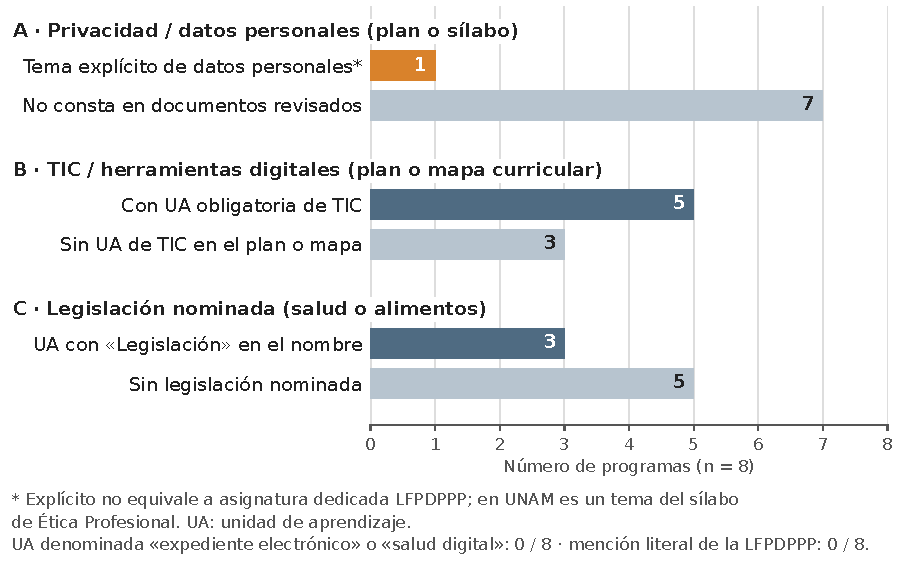
\includegraphics[width=\textwidth]{planes-nutricion.pdf}
  \caption[Presencia documental de los ejes legal-privacidad y TIC en salud
  en ocho licenciaturas públicas en nutrición]{Presencia documental de los
  ejes legal-privacidad y TIC en salud en ocho licenciaturas públicas en
  nutrición, según sus planes y mapas curriculares oficiales (Instituto
  Politécnico Nacional [IPN], 2025; Universidad Autónoma de Baja
  California [UABC], 2017; Universidad Autónoma del Estado de Morelos [UAEM], 2024;
  Universidad Autónoma de Nuevo León [UANL], s.f.;
  Universidad Autónoma Metropolitana [UAM], s.f.; Universidad de
  Guadalajara [UdeG], 2014; Universidad Juárez Autónoma de Tabasco
  [UJAT], 2018; UNAM, 2021),
  consultados el 30 de septiembre de 2026; los de la UNAM y el IPN se
  recotejaron el 8 de octubre de 2026. UA: unidad de aprendizaje
  (asignatura). «No consta» significa que el tema no aparece en el
  documento revisado; el contenido impartido en el aula no se revisó. En
  el IPN se revisó el mapa curricular oficial del plan 2025, que no
  incluye una UA de TIC. La muestra tiene fines ilustrativos.}
  \label{fig:planes-nutricion}
\end{figure}

El diagnóstico parte del supuesto de desconocimiento. Si el desconocimiento es el
problema central, preguntar a un nutriólogo si conoce la ley tiende a producir
respuestas defensivas y poco representativas de su práctica. Por eso
los instrumentos preguntan qué se hace: qué herramienta se usa, si se
entrega aviso de privacidad, si se pide consentimiento firmado, qué se
haría ante un incidente de seguridad. El cuestionario previo, contestado
antes de la sesión, recoge esa práctica sin la presión del grupo, y sus
respuestas se manejan de forma confidencial (sección~4.5). La discusión
entre colegas permite después contrastar lo que el grupo
declara en el cuestionario con lo que describe de su consulta.
 
% ────────────────────────────────────────────────────────────────────────────
\subsection{Diseño del diagnóstico}
% ────────────────────────────────────────────────────────────────────────────
 
El diagnóstico usa dos piezas del grupo focal descrito en la
sección~4.3: el cuestionario previo, que se contesta en línea
antes de la sesión, y los cuatro primeros bloques de la guía de discusión; las dos
ocurren antes de que los participantes conozcan NutriApp. El resto de
la sesión, con la presentación de las maquetas y el quinto bloque, evalúa
el diseño y se reporta en el capítulo~7. Separar los dos momentos evita que la maqueta
condicione lo que los participantes dicen de su práctica actual.
 
El cuestionario previo da las métricas base. Además del perfil del
participante (ámbito de ejercicio, años de práctica con pacientes, tipo
de consulta y número aproximado de pacientes al mes), registra la
herramienta principal del expediente, si sabe qué datos de sus pacientes
guarda y en qué lugares, si entrega algún aviso sobre el
uso de los datos, el medio por el que comparte información de pacientes
y si ha recibido solicitudes para ver, corregir o borrar sus datos.
Una tercera parte, de nueve preguntas cerradas con «No lo sé» como
respuesta válida, registra lo que el participante sabe hoy de la ley:
si recibió formación en protección de datos, si conoce la LFPDPPP y a
su autoridad, si identifica los datos de salud como sensibles y su
propio papel de responsable, y si conoce el aviso de privacidad, el
plazo para responder una solicitud del paciente, la existencia de
multas y el plazo de conservación del expediente.
Cada pregunta sobre la práctica corresponde a una
obligación de las Tablas~\ref{tab:trazabilidad-1}
y~\ref{tab:trazabilidad-2}, y cada pregunta de conocimiento se
califica contra la norma que indica el Anexo~\ref{anexo:grupo-focal}.
Con seis a ocho participantes, los
resultados se reportan como conteos, es decir, cuántos de ellos
cumplen cada obligación y cuántos conocen cada requisito, y no como
porcentajes ni promedios generalizables.

Los cuatro primeros bloques de la guía recorren la práctica actual: cómo se registra y se organiza la información del paciente en el
expediente clínico y cuánto tiempo se conserva; el aviso de privacidad,
que el responsable pone a disposición del titular antes del tratamiento
(LFPDPPP, 2025, arts.~14 y~15), y el consentimiento expreso y por
escrito para datos de salud (LFPDPPP, 2025, art.~8), que en la práctica
puede confundirse con el consentimiento del paciente para los
procedimientos clínicos (Ley General de Salud [LGS], 1984/2026, art.~51~Bis~2), aunque son
obligaciones distintas; cómo se almacenan y se comparten los datos de
salud, ligados a las medidas de seguridad, incluido el aviso al titular
cuando una vulneración afecta de forma significativa sus derechos
(LFPDPPP, 2025, art.~19); y las solicitudes de los pacientes sobre sus
datos, es decir, los derechos de acceso, rectificación, cancelación y oposición (ARCO), con el plazo de veinte días para
responder (LFPDPPP, 2025, art.~31) y la tensión entre la cancelación y
la conservación del expediente durante cinco años
(NOM-004-SSA3-2012, 2012, numeral~5.4). En cada bloque se recogen la
práctica reportada, las razones que los participantes dan para ella y
los obstáculos que encuentran para cumplir.
 
El análisis sigue el procedimiento de la sección~4.3.5: los conteos del
cuestionario previo se contrastan con lo que los participantes describen en
la discusión, y ambos se cruzan con las obligaciones de las tablas de
trazabilidad. El resultado es la lista de obligaciones presentes y
ausentes en la práctica reportada, con las razones y los obstáculos
que la explican. Esa lista es la línea base contra la que el capítulo~7 valora el diseño.
 
\subsection{Resultados del diagnóstico}
 
La línea base se integró con el cuestionario previo, que los ocho
participantes analizados respondieron el 23 de octubre de 2026 antes de
la sesión, y con los cuatro primeros bloques de la discusión. Los
conteos completos, pregunta por pregunta, están en el
Anexo~\ref{anexo:previo-resultados}; aquí se leen contra las
obligaciones de las Tablas~\ref{tab:trazabilidad-1}
y~\ref{tab:trazabilidad-2}. De las nueve personas que asistieron, una
se excluyó del análisis (sección~4.3.4).
 
\paragraph{Perfil de los participantes}
Cuatro ejercen en consulta privada, dos en una institución y dos en
ambos ámbitos; en la sesión, dos describieron práctica en un hospital
público y una en salud ocupacional de empresa. Cuatro llevan menos de
dos años atendiendo pacientes y cuatro entre dos y cinco. Tres
consultan sobre todo en persona, uno en línea y cuatro de forma mixta;
tres atienden menos de veinte pacientes al mes, uno entre veinte y
cincuenta, y cuatro entre cincuenta y uno y cien.
 
\paragraph{Herramientas y práctica actual}
En el cuestionario, tres llevan el expediente principal en una hoja de
cálculo, tres en un software especializado para nutriólogos, uno en un
documento de texto y una en una aplicación de notas. La discusión
matizó ese conteo: seis de los ocho usan algún software especializado
---tres productos comerciales y uno hecho a la medida---, pero en todos
los casos convive con archivos de uso general (documentos de texto,
hojas de cálculo, carpetas en la computadora, nube personal o un disco
duro externo); en la práctica hospitalaria pública, el expediente es
impreso. La información reside en la computadora (cinco), en la nube de
consumo (cinco), en el servidor del software (cuatro), en el teléfono
(uno) y en papel (uno); seis dicen saber qué datos guardan y en qué
lugares, y dos «más o menos». La protección declarada es la contraseña
del dispositivo (cinco), la del archivo o la aplicación (cuatro) y el
respaldo periódico (tres); nadie marcó cifrado ni usuarios individuales
por persona, y una respuesta no declara protección alguna. Nadie
comparte el expediente con asistentes: en el único caso con apoyo
externo, quien confirma las citas ve solo el nombre y el teléfono. La
compartición con terceros es esporádica ---cuatro la harían o la han
hecho por WhatsApp y dos por correo; tres no comparten--- y, en los
casos relatados en la discusión, medió el aviso al paciente o una
firma.
 
\paragraph{Aviso de privacidad}
Uno de los ocho entrega un aviso por escrito o en pantalla, uno lo
explica de palabra y seis no lo tocan. En la discusión aparecieron los
dos mecanismos existentes: un aviso que el paciente firma en una
plataforma de firma electrónica y una casilla de aceptación en el
formulario previo a la consulta; con pacientes menores de edad, en
ambos casos firma el padre, la madre o el tutor. Preguntados de forma
cerrada por el obstáculo, tres lo atribuyen a desconocimiento (dos no
sabían que era obligatorio y uno no sabía qué debe decir), dos a que su
herramienta no lo incluye y uno a falta de tiempo; dos declaran ya
hacerlo (Anexo~\ref{anexo:salida-resultados}).
 
\paragraph{Consentimiento por escrito para datos de salud}
Ninguno recaba un consentimiento específico para los datos de salud:
dos lo integran al consentimiento del tratamiento clínico y seis no
piden ninguna autorización firmada. La distinción entre el
consentimiento clínico y el de datos (sección~3.2) no apareció en la
discusión ni en los mecanismos descritos.
 
\paragraph{Derechos ARCO y medidas de seguridad}
En el cuestionario, nadie reporta haber recibido solicitudes para ver,
corregir o borrar datos; en la discusión, una participante relató dos
solicitudes de acceso atendidas con firma de por medio. La diferencia
ilustra el contraste entre el registro cerrado y el relato que busca la
triangulación (sección~4.3.5). Ante la petición hipotética de borrar
toda la información, quienes respondieron la resolverían borrando el
expediente, con un documento o un escrito del paciente como constancia;
nadie mencionó la conservación mínima ni el bloqueo. Ninguno de los
ocho conoce el plazo legal de respuesta ni identifica a la autoridad
vigente ---una respuesta nombró al INAI y dos a la COFEPRIS---, y nadie
conoce el orden de magnitud de las multas, aunque cuatro saben que
existen. La conservación muestra la brecha más clara entre lo que se
sabe y lo que se hace: seis saben que el expediente clínico se conserva
cinco años, pero solo uno declara conservarlo cinco años o más; cuatro
lo conservan de uno a cuatro años, uno menos de un año y dos lo
conservan indefinidamente o sin regla definida, y en la discusión nadie
ha depurado un expediente, «por si el paciente regresa» o hasta que
falte espacio. Ante la pérdida de un equipo o un acceso no autorizado,
ninguno tiene un procedimiento: las respuestas se orientan a recuperar
la información desde la nube o el respaldo, solo una describe contención
(cerrar sesiones y cambiar contraseñas) y solo una, al preguntarlo,
avisaría a sus pacientes tras confirmar una filtración. Cuatro de los
ocho no han recibido formación alguna en protección de datos, y nadie
declara conocer la ley al punto de aplicarla en su consulta.
 
\paragraph{Obligaciones presentes y ausentes en la práctica reportada}
Leída contra las Tablas~\ref{tab:trazabilidad-1}
y~\ref{tab:trazabilidad-2}, la práctica reportada presenta de forma
parcial las medidas de seguridad básicas (obligación~III: contraseñas y
respaldo, sin cifrado) y el conocimiento del propio inventario
(VI); el acceso de hecho es individual (IV), pero sin usuarios propios
ni registro de quién consulta qué expediente (VIII, ausente en todas
las herramientas descritas). Están ausentes el aviso de privacidad
sistemático (II), el consentimiento específico para datos de salud (I),
el procedimiento ante vulneraciones con aviso al titular (V), la
gestión de solicitudes con plazo y registro (VII) y la regla de
conservación aplicada (IX). El uso de nube y de software de terceros es
general, sin verificación declarada de las condiciones del proveedor
(XI); una participante cambió de herramienta precisamente por
desconfianza en el acceso del personal del proveedor a los datos. La
obligación~X no se midió en campo, porque la pregunta prevista no se
incluyó en el formulario aplicado (Anexo~\ref{anexo:cuestionario}), y
se evalúa solo con el análisis documental. Los obstáculos que los
participantes reportan son de desconocimiento y de herramienta, no de
rechazo a la obligación. Esta lista es la línea base contra la que el
capítulo~7 valora el diseño.
 
% ============================================================
% CAPÍTULO 4 — METODOLOGÍA (grupo focal con expertos)
% Parámetros de campo: sesión en línea del 23-oct-2026; asistieron 9,
% se analizan 8; moderó el asesor por ausencia del facilitador externo.
% Sin entradas bibliográficas nuevas.
% ============================================================
\section{Metodología}
% ═══════════════════════════════════════════════════════════════════════════
 
La evidencia de este caso se produce con un procedimiento que otro
investigador pueda repetir con los mismos materiales y llegar a
conclusiones comparables. Las secciones que siguen precisan el tipo de
estudio, las fuentes documentales, los instrumentos de campo, la forma
de evaluar el artefacto y las condiciones éticas del trabajo.
 
% ------------------------------------------------------------
\subsection{Tipo de estudio y enfoque metodológico}
% ------------------------------------------------------------
 
\subsubsection{Clasificación}
 
Este trabajo se clasifica como investigación aplicada de diseño
(\textit{design science research}) con estrategia de caso de estudio.
La investigación de diseño produce conocimiento sobre cómo construir un
artefacto que atienda un problema de la práctica profesional, a
diferencia de la investigación descriptiva, cuyo propósito es comprender
fenómenos existentes. Hevner et al. (2004) definen su objetivo como
\textit{``create innovations that define the ideas, practices, technical
capabilities, and products through which the analysis, design,
implementation, management, and use of information systems can be
effectively and efficiently accomplished''} (p.~76).
 
El proceso sigue las seis actividades que Peffers et al. (2007) proponen
para este tipo de investigación. La identificación del problema y la
definición de objetivos ocupan los capítulos~1 a~3, con una entrada
centrada en el problema que plantea el marco normativo: el diagnóstico
empírico del capítulo~3 se recoge en la misma sesión que la evaluación
y sirve de línea base (sección~3.2), no de insumo del diseño; los
capítulos~2 (secciones~2.4 y~2.5), 5 y~6 desarrollan el
artefacto. La demostración, que en Peffers et al.
consiste en mostrar que el artefacto resuelve una instancia del
problema, se hace en el capítulo~6 con maquetas navegables de la
interfaz y una prueba piloto con el grupo
focal. El capítulo~7 evalúa con los tres métodos de la
sección~4.4.2: casos de prueba de aceptación que se ejecutan sobre las
maquetas, revisión por expertos de los participantes del grupo focal y observación de lo que
los participantes dicen y hacen frente a ellas; verifica además la
trazabilidad de las once obligaciones (sección~7.2) y estima el costo de
operar el diseño (sección~7.3). Este
documento constituye la comunicación. El ciclo no incluye la
implementación del sistema ni su evaluación en operación, porque el
alcance termina en el diseño; el capítulo~8 propone la ruta para
quien continúe el trabajo.
 
La estrategia de caso de estudio se adopta porque el contexto es
relevante para el fenómeno y los límites entre uno y otro no son
nítidos, condición en la que Yin (2018) la considera apropiada
(p.~15). Las prácticas de manejo de datos en el sector de nutrición y
el grado en que sus profesionales conocen la Ley Federal de Protección de Datos Personales en Posesión de los Particulares (LFPDPPP) no se entienden
fuera del contexto profesional, normativo y tecnológico en que
ocurren. El consultorio de nutrición de práctica privada es la unidad de
análisis; NutriApp es el artefacto diseñado para él.
 
\subsubsection{Alcance: el diseño como plano técnico}
 
Este trabajo abarca el diseño de la solución; la implementación y la
evaluación en producción quedan fuera. Peffers et al. (2007) admiten
como artefacto de investigación de diseño cualquier objeto diseñado en
el que esté incorporada una contribución de investigación. El artefacto
de este caso es el paquete de diseño. Lo integran el marco normativo y
técnico del capítulo~2, la matriz de trazabilidad entre obligaciones
y requerimientos, la arquitectura de servicios, los diagramas de
ingeniería, el modelo de datos, los requerimientos del producto mínimo
viable, los casos de prueba de aceptación y las maquetas navegables de
interfaz. El paquete se evalúa con casos de prueba y con la revisión
de expertos del grupo focal, y se documenta con el detalle necesario
para que una fase de desarrollo lo tome como punto de partida sin
repetir el análisis, sea por el autor o por un tercero al que se
transfiera (sección~4.5). Las maquetas son representaciones de pantalla
sin lógica de negocio ni datos reales; ninguna decisión de arquitectura
se desplegó ni se probó.
 
% ------------------------------------------------------------
\subsection{Investigación documental}
% ------------------------------------------------------------
 
\subsubsection{Criterios de selección del marco legal}
 
El marco normativo del capítulo~2 se construyó con fuentes primarias
(la LFPDPPP de 2025, el Reglamento de 2011, la Ley General de Salud,
la NOM-004-SSA3-2012 y la NOM-024-SSA3-2012) y con fuentes secundarias:
literatura académica y documentación técnica de los estándares
internacionales. Las jurisdicciones comparadas se seleccionaron con
cuatro criterios: relevancia regional, madurez normativa, contraste
metodológico y disponibilidad de la documentación oficial en español,
inglés o portugués.
 
Por relevancia regional se priorizaron jurisdicciones de América
Latina, que comparten tradición jurídica con México y sirven de
referencia para la propuesta. Por madurez normativa se incluyeron el
Reglamento General de Protección de Datos (GDPR) aplicado en Alemania y la Health Insurance Portability and Accountability Act (HIPAA) estadounidense, ordenamientos
consolidados y con experiencia documentada. El contraste metodológico
llevó a regímenes con enfoques distintos al mexicano, para que las
fortalezas y debilidades de la LFPDPPP se vieran por comparación.
 
\subsubsection{Estructura de la revisión comparada}
 
Las nueve categorías de la revisión son comunes a todas las
jurisdicciones y forman las filas de la Tabla~\ref{tab:comparativo-normativo}
(sección~2.2.5). Son la ley principal vigente, la autoridad reguladora,
el tratamiento de los datos de salud como sensibles, el consentimiento
expreso por escrito, la notificación de vulneraciones, la portabilidad de
datos, las sanciones máximas, la alineación con el GDPR y el marco
técnico para software de salud. Las categorías se eligieron por su relación con las decisiones de
diseño de NutriApp.
 
\subsubsection{Verificación de fuentes y fecha de corte}
 
Las citas a artículos de la LFPDPPP, de su Reglamento y de la Ley
General de Salud, y a numerales de las NOM, se cotejaron contra el
texto publicado por la fuente oficial: Cámara de Diputados, Diario
Oficial de la Federación y sitios de los organismos emisores. Las citas
a la legislación extranjera se tomaron de los textos consolidados que
publican sus autoridades. Las ediciones de los estándares
internacionales se tomaron como estaban vigentes al 31 de enero de
2026, fecha de corte de este trabajo: las modificaciones normativas
posteriores se mencionan cuando afectan al análisis, pero no se
incorporan a él. Un supuesto se declara de forma expresa. El decreto
de 2025 abroga la ley de 2010 y otras cuatro disposiciones sin
mencionar el Reglamento de 2011 (LFPDPPP, 2025, Transitorio Segundo),
y ordena al Ejecutivo Federal adecuar los reglamentos en los noventa
días naturales siguientes a su entrada en vigor (Transitorio Décimo
Segundo). Al corte de este trabajo esa adecuación no se había
publicado en el Diario Oficial, por lo que el Reglamento de 2011 se
aplica como texto vigente en lo que es compatible con la nueva ley.
Si la adecuación cambia los artículos aquí citados
(20, 48, 50 a 52, 54, 57, 61, 64, 65, 107 y 108), las tablas de trazabilidad
deberán actualizarse. La fecha de corte fija el estado del derecho
analizado. Los precios de los servicios de nube, mensajería y pagos
son la excepción: se tomaron el 24 de septiembre de 2026, porque el
costo de operar el diseño se estima con las tarifas vigentes a la
fecha de redacción; los de la competencia, el 18 de octubre de 2026.
 
% ------------------------------------------------------------
\subsection{Investigación de campo: grupo focal con expertos}
% ------------------------------------------------------------
 
\subsubsection{Diseño del estudio de campo y población}
 
La investigación de campo usa un grupo focal con expertos. La decisión
se tomó con el tutor por el tipo de evidencia que el caso necesita:
el objeto del estudio de campo es la forma en que los nutriólogos
manejan los datos de sus pacientes y lo que entienden por cumplir con
la ley, y la discusión entre profesionales que atienden pacientes
recoge esa información mejor que un cuestionario cerrado. Participan
nutriólogos en ejercicio porque esa práctica de consultorio solo la
puede describir quien ya atiende pacientes.
 
La población son nutriólogos con práctica clínica activa, en consulta
privada o institucional; la docencia no es requisito. Se incluyen
participantes mayores de edad que atienden pacientes al momento del
estudio y que aceptan, en el consentimiento informado previo a la
sesión, participar y que la sesión se transcriba de forma automática;
se excluyen quienes no atienden pacientes, porque las preguntas se
refieren a su experiencia clínica.
 
Se formó un solo grupo. La invitación se envió por mensaje directo en
Doctoralia a diez nutriólogos con consulta activa, para asegurar al
menos seis participantes; asistieron nueve. La sesión se realizó el
viernes 23 de octubre de 2026, a las 14:00~h (hora de la Ciudad de
México), en línea por Google Meet, con su función de transcripción
automática, y duró 60~minutos. El diseño preveía la conducción por un
facilitador externo con experiencia en grupos focales, que recibió con
anticipación los objetivos de la sesión, la guía de discusión y las
conclusiones por corroborar o desechar; una ausencia imprevista el
mismo día llevó a que la sesión la moderara el asesor de la tesis, con
esos mismos materiales. El cambio consta en la minuta
(Anexo~\ref{anexo:minuta}) y se declara como limitación
(secciones~4.4.3 y~8.3). El diseño de los instrumentos se
fundamenta en la metodología de grupos focales y de construcción de
instrumentos de la investigación en ciencias sociales
(Hernández-Sampieri et al., 2014) y se sometió a la revisión de un
colaborador externo con experiencia en trabajo de campo, ajeno al grupo
focal, antes de su aplicación. El procesamiento de los datos y la
interpretación de los resultados en relación con el marco normativo
están a cargo del autor, que asistió a la sesión para presentar las
maquetas y el cierre de requisitos, sin intervenir en la discusión.
 
\subsubsection{Instrumentos}
 
Los materiales del estudio de campo son cuatro y se aplican en este
orden: el consentimiento informado, el cuestionario previo, la guía de
discusión y una encuesta de salida anónima que, después de la sesión,
registra la valoración de las funciones mostradas, la percepción de la
carga de trabajo que pedirían y los cambios que cada participante prevé
en su práctica. Los cuatro se reproducen en el
Anexo~\ref{anexo:grupo-focal}. El \textit{consentimiento informado} se
recabó antes de la sesión; con su aceptación, cada participante
autorizó su intervención y la transcripción automática de la sesión.
 
El \textit{cuestionario previo} es breve y se contesta antes de la
sesión en Google Forms, sin inicio de sesión ni registro del correo; en
la aplicación se envió junto con el consentimiento informado, en un
solo formulario (sección~4.5).
Recoge el perfil del participante (ámbito de ejercicio, años de
práctica con pacientes, tipo de consulta y número aproximado de
pacientes al mes) y su práctica actual con datos de pacientes: la
herramienta principal del expediente, si sabe qué datos de sus
pacientes guarda y en qué lugares, si entrega algún aviso sobre el uso
de los datos, el medio por el que comparte información de pacientes y
si ha recibido solicitudes para ver, corregir o borrar sus datos.
Cierra con nueve preguntas cerradas sobre lo que el participante sabe
de la ley, con «No lo sé» como respuesta válida; el formulario aclara
que no es un examen y que nadie ve las respuestas individuales. Sus
respuestas forman la línea base del capítulo~3, de práctica y de
conocimiento, se recogen antes de que el participante conozca NutriApp
y se manejan de forma confidencial.
 
La \textit{guía de discusión} organiza la sesión en cinco bloques con
preguntas abiertas de práctica antes que de conocimiento, para que el
participante describa lo que hace en consulta. Los cuatro primeros se
conducen antes de mostrar cualquier material de NutriApp: el expediente
clínico en la práctica actual; el aviso de privacidad y el
consentimiento; el almacenamiento y la compartición de datos de salud;
y las solicitudes de los pacientes sobre sus datos. El quinto recoge
opiniones sobre las funciones de NutriApp después de una presentación
breve de las maquetas, con perfiles ficticios. Al presentarlas se
indica que NutriApp es una herramienta que no asume las obligaciones
legales del nutriólogo, quien sigue siendo el responsable del
tratamiento de los datos de sus pacientes.
 
Los grupos focales se emplean como técnica de recolección cualitativa
reconocida en la metodología de la investigación (Hernández-Sampieri
et al., 2014). El cuestionario previo agrega un registro cerrado que
describe la práctica antes de conocer el diseño.
 
\subsubsection{Procedimiento de sesión}
 
La sesión siguió este orden en 60~minutos; el moderador definió la
dinámica y el tiempo de cada bloque, salvo los diez minutos finales. La
línea base se recoge antes de mostrar cualquier material de NutriApp,
para que la maqueta no condicione las respuestas sobre la práctica
actual.
 
\begin{enumerate}
  \item Apertura, comprobación del consentimiento y del cuestionario
    previo e inicio de la transcripción automática.
  \item Bloques 1 a 4 de la guía de discusión: el expediente clínico en
    la práctica actual; el aviso de privacidad y el consentimiento; el
    almacenamiento y la compartición de datos de salud; y las
    solicitudes de los pacientes sobre sus datos.
  \item Presentación breve de las maquetas de NutriApp.
  \item Bloque 5: opiniones sobre las funciones de NutriApp.
  \item Cierre, en los últimos diez minutos: una exposición breve de los
    requisitos mínimos de la LFPDPPP para el consultorio y respuesta a
    preguntas frecuentes. Va al final, una vez concluida la discusión,
    para no influir en lo que los participantes reportan; tras la
    sesión se envía a los participantes la encuesta de salida y el
    documento de referencia comprometido en el cierre
    (Anexo~\ref{anexo:referencia}).
\end{enumerate}
 
La información de la sesión se maneja de forma confidencial, y la
transcripción automática sigue el procedimiento de la sección~4.5. El
anexo del estudio de campo es la minuta de la sesión, que elaboró el
autor a partir de la transcripción anonimizada ante el cambio de
moderador (Anexo~\ref{anexo:minuta}). El quinto bloque no llegó a
desarrollarse como discusión, porque tras la presentación de las
maquetas no hubo intervenciones; las opiniones sobre las funciones se
recogieron con la encuesta de salida (sección~7.1).
 
\subsubsection{Muestra}
 
La muestra fue no probabilística y dirigida: nutriólogos con práctica
clínica, elegidos por su ejercicio profesional y no por su
representatividad estadística. Asistieron nueve; el análisis considera
a ocho, porque una participante atendió consulta durante la sesión, no
intervino en la discusión y contestó el cuestionario previo horas
después de esta, cuando ya no registraba la práctica previa al contacto
con el diseño; sus respuestas se documentan, fuera de los conteos, en
el Anexo~\ref{anexo:previo-resultados}. El tamaño queda dentro del
rango de seis a diez participantes que se recomienda para grupos de
enfoque sobre asuntos de la práctica cotidiana (Creswell, 2005, como se
citó en Hernández-Sampieri et al., 2014, p.~409) y permitió que todos
intervinieran en una sesión de 60 minutos.
El caso es único y los participantes son fuentes de evidencia dentro
de él, en el sentido de Yin (2018); el tamaño de la muestra no busca
inferencia estadística sobre el gremio. Los patrones que surjan,
contrastados con la literatura y con el marco normativo, se presentan
como evidencia exploratoria del grupo estudiado.
 
\subsubsection{Análisis y triangulación}
 
El cuestionario previo se procesa con estadística descriptiva:
frecuencias absolutas por pregunta y por perfil; en las preguntas de
conocimiento se cuenta cuántos participantes responden conforme a la
norma, cuántos responden otra cosa y cuántos marcan «No lo sé». Con seis a ocho
participantes no se calculan porcentajes ni se generalizan
proporciones. La transcripción anonimizada se codifica por los bloques
de la guía; dentro de cada bloque se agrupan las prácticas
reportadas, las razones que los participantes dan para ellas y los
obstáculos que identifican.
 
La triangulación contrasta lo que los participantes declaran en el
cuestionario previo con lo que describen en la discusión, para detectar
diferencias entre lo que se dice y lo que se hace, y entre lo que se
sabe de la ley y lo que se practica; cruza las prácticas
reportadas con las obligaciones de las Tablas~\ref{tab:trazabilidad-1}
y~\ref{tab:trazabilidad-2}, para identificar qué obligaciones están
presentes en la práctica reportada y cuáles faltan; y compara esos
hallazgos con la literatura sobre protección de datos en profesiones de
salud en México y América Latina. Los resultados del
diagnóstico se presentan en el capítulo~3; las opiniones sobre las
funciones de NutriApp, en el capítulo~7. El cruce entre el
cuestionario y la discusión se hace en el nivel del grupo, sin
emparejar las respuestas y las intervenciones de una misma persona,
conforme al compromiso del consentimiento (sección~4.5).
 
% ------------------------------------------------------------
\subsection{Diseño y evaluación del artefacto}
% ------------------------------------------------------------
 
\subsubsection{Trazabilidad: de requisito legal a decisión técnica}
 
La trazabilidad liga cada componente técnico de NutriApp que atiende
una obligación con el requisito normativo que lo origina; los
componentes funcionales o comerciales sin fundamento normativo quedan
fuera de la matriz. El procedimiento tiene tres pasos. Se identifica
la obligación en la LFPDPPP, su Reglamento, la NOM-004 o la NOM-024,
con el artículo o numeral que la establece. Se formula después el
requerimiento técnico como una capacidad que pueda comprobarse: qué
debe hacer el sistema, no cómo. Por último, se selecciona el componente
que satisface ese requerimiento con el menor nivel de complejidad
suficiente, respaldado por el pilar de seguridad del Amazon Web Services
(AWS) Well-Architected Framework (AWS, 2024b) o por los estándares de la
sección~2.5.6. El resultado se
documenta en las Tablas~\ref{tab:trazabilidad-1}
y~\ref{tab:trazabilidad-2} y se materializa en la arquitectura del
capítulo~5.
 
\subsubsection{Demostración y evaluación}
 
Las maquetas navegables, construidas en Figma Make a partir de los
requerimientos del capítulo~6, demuestran el artefacto junto con la
prueba piloto en la sesión del grupo focal. La evaluación
combina tres métodos: pruebas y observación, afines a dos de los
métodos que Hevner et al. (2004) reconocen para artefactos de diseño, y
revisión por expertos.
 
Para las \textit{pruebas} se derivan casos de aceptación de los
requerimientos. Cada caso indica la obligación que lo origina, la
precondición, los pasos, el resultado esperado conforme a la ley y la
evidencia que debe verse en la maqueta. El autor ejecuta los casos como
recorrido sobre las maquetas y los califica en tres valores: refleja
el diseño, lo refleja parcialmente o no lo refleja. El capítulo~6
presenta los tres casos del producto mínimo viable (consentimiento del
paciente, alta de un expediente y solicitud de cancelación) y el
capítulo~7 reporta su resultado. Un resultado de «no refleja» se
reporta como hallazgo y señala la distancia entre la maqueta y el
diseño.
 
Los nutriólogos del grupo focal hacen la \textit{revisión por
expertos} con sus opiniones sobre las funciones de las maquetas,
previstas para el quinto bloque de la guía de discusión y recogidas, en
la aplicación, con la encuesta de salida (sección~7.1). La
\textit{observación en el caso} recoge lo que dicen y hacen frente a
las maquetas durante la sesión.
 
\subsubsection{Alcance y limitaciones}
 
Las limitaciones se declaran por su origen: la evaluación empírica, el
alcance normativo y la representatividad de los participantes. Las
maquetas de NutriApp son representaciones de interfaz, en los términos
de la sección~4.1.2, y las decisiones de arquitectura son propuestas
fundamentadas que ningún tercero independiente ha auditado. Los casos
de prueba comprueban que la maqueta muestre el flujo previsto, no que
un sistema lo ejecute, y los ejecuta y califica el propio autor, de modo
que constituyen una autoevaluación del diseño.
 
El análisis normativo se centra en la LFPDPPP, su Reglamento, la
NOM-004 y la NOM-024. Una implementación requeriría análisis
adicionales en materia fiscal, laboral y sanitaria.
 
Los participantes fueron nueve nutriólogos con práctica clínica (ocho
analizados), reunidos en una sola sesión y seleccionados de forma
dirigida. Los
resultados describen a ese grupo y constituyen evidencia exploratoria,
sin inferencia sobre el gremio. Quienes aceptan participar en un
estudio sobre protección de datos, reclutados en un directorio en línea,
pueden tener más interés en el tema y mayor uso de herramientas digitales
que el promedio de sus colegas, y la perspectiva del paciente, titular
de los datos, no está representada en el estudio de campo.
 
% ------------------------------------------------------------
\subsection{Consideraciones éticas y confidencialidad}
% ------------------------------------------------------------
 
El estudio de campo sigue los principios de la investigación con seres
humanos. La participación es voluntaria y puede
abandonarse en cualquier momento sin consecuencia; cada participante
acepta, en el consentimiento informado previo a la sesión,
participar y que la sesión se transcriba de forma automática, y declara ser
mayor de edad. El cuestionario previo se contesta en Google Forms, sin
inicio de sesión. En la aplicación, el aviso de participación y el
cuestionario se enviaron en un solo formulario, que registró el nombre
de cada participante junto con sus respuestas para coordinar la sesión
y el pago; no pidió cédula profesional ni correo. Antes del análisis,
el autor separó los nombres de las respuestas, asignó a cada
participante un código y conservó los nombres solo en el registro de
pagos, de modo que ni el análisis ni los resultados identifican a
nadie; la encuesta de salida pidió también el nombre y se trató de la
misma forma. Cada
participante recibe \$350 pesos como pago por su tiempo y su experiencia; el
monto no depende de sus respuestas. La sesión es
confidencial; la transcripción automática se anonimiza antes de
elaborar la minuta de la sesión, que no identifica a los participantes;
el audio no se graba ni se conserva, y la transcripción original se
elimina una vez elaborada la minuta. Los resultados se reportan en
forma agregada o con citas sin atribución, y el
Anexo~\ref{anexo:grupo-focal} incluye la minuta de la sesión y los
resultados agregados de los cuestionarios.
 
El uso de las maquetas de NutriApp en la sesión es demostrativo.
Ningún dato real de pacientes se captura en ellas: todos los perfiles
son ficticios y llevan la etiqueta \textit{(USUARIO DE PRUEBA)} en los
campos de nombre, y así se comunica por escrito a los participantes.
Los datos personales que sí se tratan en el estudio son los de los
participantes, en particular lo que expresan durante la sesión, y a ellos se les
entrega el aviso de privacidad correspondiente.
 
El autor declara que, concluido el caso, el paquete de diseño podrá
transferirse o licenciarse a un tercero para su implementación.
Ninguna organización externa financió ni condicionó este trabajo, y
ningún participante tiene relación con esa eventual transferencia. El
colaborador externo que revisa los instrumentos antes de su aplicación lo hace
sin contraprestación, no participa en la interpretación de los
resultados y no tiene interés en NutriApp ni en su transferencia. La
sesión la moderó el asesor de la tesis, ante la ausencia imprevista del
facilitador externo previsto; el asesor tampoco tiene interés en
NutriApp ni en su transferencia, y la pérdida de independencia del
moderador se declara como limitación (sección~8.3).

% ═══════════════════════════════════════════════════════════════════════════
\section{Diseño de la solución}
% ═══════════════════════════════════════════════════════════════════════════
 
El diseño de NutriApp lleva las obligaciones y el marco técnico del
capítulo~2 a una arquitectura de servicios, que comprende la
infraestructura elegida, los diagramas de ingeniería que la
representan y el modelo de datos que la sustenta (alcance declarado
en la sección~4.1.2). Los componentes se distinguen por su origen.
Unos atienden una obligación identificada en las
Tablas~\ref{tab:trazabilidad-1} y~\ref{tab:trazabilidad-2}. Otros
exceden lo que la norma exige por decisión de diseño, como la región
primaria en México. Los demás son funcionales o comerciales y carecen
de fundamento normativo propio, como el catálogo, la reserva de citas
y el módulo social.
 
% ─────────────────────────────────────────────────────────────────────────
 
\subsection{Infraestructura en Amazon Web Services: KMS, Cognito, Lambda, RDS}
% ─────────────────────────────────────────────────────────────────────────

NutriApp se diseña sobre Amazon Web Services (AWS) bajo el modelo de
responsabilidad compartida de la sección~2.5.1 (AWS, 2023b). AWS
responde por la seguridad de la infraestructura
física y de red, y el cliente por la configuración de los servicios,
el control de acceso y el cifrado. La elección
del proveedor obedece a criterios de diseño. La región AWS Mexico
(Central), abierta en enero de 2025, permite alojar el tratamiento
principal dentro del país (AWS, 2025). Las auditorías independientes
que AWS mantiene bajo ISO/IEC~27001, ISO/IEC~27018 y SOC~2 Tipo~II
(AWS, 2023a) sirven como evidencia de las medidas de seguridad que el
artículo~52 del Reglamento exige al proveedor de cómputo en la nube
(Reglamento de la Ley Federal de Protección de Datos Personales en Posesión de los Particulares [RLFPDPPP], 2011, art.~52, fracc.~II). El pilar de seguridad del AWS
Well-Architected Framework (AWS, 2024b) documenta buenas prácticas para las
decisiones de arquitectura de este capítulo. La región primaria es
\texttt{mx-central-1} por decisión de diseño; la ley no exige
localización. Cognito, el cómputo y los datos residen en esa región.
El borde que muestra la Figura~\ref{fig:aws-a} (Route 53, CloudFront,
la ACL web global de WAF, Shield y el certificado de ACM) es global y
opera fuera de ella; la ACL web regional de WAF, que protege a API
Gateway, sí está en \texttt{mx-central-1}.
Amazon SES no está disponible en \texttt{mx-central-1}, por lo que los
avisos por correo, sin contenido clínico, salen de SES en
\texttt{us-east-1} (Figura~\ref{fig:aws-b}), fuera del territorio
nacional. Esos servicios se transparentan al nutriólogo como
subcontrataciones del encargado (sección~2.5.1).

Los componentes se describen por capas. La justificación normativa de
cada control está en la sección~2.5 y en la Tabla~\ref{tab:stack}.

\textbf{Entrega de contenido.} Amazon CloudFront sirve la interfaz web
(React, Vite y TypeScript) desde Amazon S3, con caché en sus puntos de
presencia y certificado TLS (Transport Layer Security) gestionado por AWS Certificate Manager. El
tráfico entre el dispositivo y la plataforma se transmite cifrado con
TLS~1.3 (Rescorla, 2018).

\textbf{Protección perimetral.} AWS WAF inspecciona el tráfico entrante
con reglas administradas contra inyección SQL, secuencias de comandos
entre sitios y patrones de ataque conocidos, y aplica una regla basada
en tasa que limita las solicitudes por dirección IP en una ventana
definida. AWS Shield Standard mitiga los ataques de denegación de
servicio distribuido.

\textbf{Lógica de aplicación.} Amazon API Gateway expone los servicios
REST, valida los tokens emitidos por Amazon Cognito en las rutas
privadas (las del catálogo son públicas) e invoca las funciones Lambda mediante integración \textit{Lambda proxy} (AWS,
s.f.-m).
Las funciones AWS Lambda (Node.js) ejecutan la lógica de negocio con
límites de concurrencia que acotan las ejecuciones simultáneas. La API
recibe y devuelve solo los campos que cada pantalla necesita, en
atención al principio de proporcionalidad (Ley Federal de Protección de Datos Personales en Posesión de los Particulares [LFPDPPP], 2025, arts.~5 y~12).

\textbf{Identidad y acceso.} Amazon Cognito gestiona el registro, la
confirmación del correo, la autenticación multifactor (MFA), la
emisión de tokens y el bloqueo tras intentos fallidos consecutivos,
con el nivel de aseguramiento AAL2 (\textit{Authenticator Assurance
Level}~2) como nivel objetivo (sección~2.5.2). El segundo factor es un
código TOTP (\textit{time-based one-time password}) generado por una
aplicación de autenticación, que Cognito ofrece como MFA por
\textit{software token} y que el profesional inscribe con un código QR
en la pantalla \texttt{MFASetup} (AWS, s.f.-a); la MFA por SMS
permanece desactivada y la \textit{passkey} se admite como
autenticador adicional (AWS, 2024a). El grupo de usuarios se configura
con MFA opcional, y la obligatoriedad para nutriólogo, docente y
administrador la impone la aplicación: \texttt{MFASetup} es un paso del
registro que no puede omitirse, y la API rechaza toda ruta clínica o
administrativa de una cuenta de esos roles sin autenticador inscrito.
La pérdida del dispositivo se resuelve con un procedimiento operado
por el administrador de NutriApp (verificación por el correo
confirmado y los datos declarados, restablecimiento del factor y nueva
inscripción), que queda con folio en el registro de auditoría. Cada rol
usa un cliente de aplicación de Cognito propio, porque la vigencia de
los tokens se fija por cliente: quince minutos para el token de acceso
y doce horas para el de actualización en nutriólogo, docente y
administrador; sesenta minutos y treinta días en el paciente. El
bloqueo por intentos fallidos sigue el comportamiento documentado de
Cognito, que tras cinco intentos fallidos con contraseña bloquea al
usuario un segundo y duplica la espera en cada intento siguiente hasta
unos quince minutos (AWS, s.f.-r); los inicios de sesión exitosos y
fallidos quedan en CloudTrail y, mediante un disparador posterior a la
autenticación, en el \texttt{audit\_log}. Los permisos se asignan por
rol (nutriólogo, paciente, docente y administrador): cada función
Lambda autoriza la solicitud a partir del grupo de Cognito que trae el
token y del nutriólogo responsable del registro solicitado, y las
tablas clínicas de PostgreSQL añaden seguridad por filas para que
ninguna consulta cruce expedientes de distintos responsables. El rol
de auditoría de la sección~2.5.4 no es un usuario de la aplicación sino
un rol de IAM de solo lectura de la operación de NutriApp, con MFA y
acceso a los depósitos de registros, sin acceso a RDS; su uso queda en
CloudTrail. La cuenta Students es un nutriólogo con permisos acotados
a pacientes ficticios (sección~6.2.5).

\textbf{Datos y llaves.} Amazon RDS para PostgreSQL almacena
expedientes, consentimientos, solicitudes de derechos de acceso, rectificación, cancelación y oposición (ARCO) y el
\texttt{DeclarationLog}. Amazon S3 guarda los adjuntos, como planes en
PDF e imágenes de progreso, con versionado y Object Lock durante el
plazo de conservación de la NOM-004-SSA3-2012 (sección~2.5.5); las reglas de
ciclo de vida actúan después de ese plazo. AWS Key Management Service (KMS)
custodia las llaves con el esquema por envolvente de la
sección~2.5.3. La llave de datos de cada expediente se genera bajo la
llave maestra del entorno y solo se conserva cifrada, en la columna
\texttt{llave\_datos\_cifrada} del expediente; en claro existe
únicamente en la memoria de la función Lambda mientras atiende una
solicitud. Con ella se cifran en la aplicación, con AES-256-GCM
mediante el AWS Encryption SDK para JavaScript (AWS, s.f.-b), las
columnas clínicas de \texttt{expediente}, \texttt{nota},
\texttt{medicion} y \texttt{plan\_alimentacion} y cada adjunto antes
de subirlo a S3, además del cifrado del lado del servidor de RDS y de
S3 bajo la llave maestra; así, destruir la llave de datos vuelve
ilegible el expediente completo, adjuntos incluidos (sección~2.5.5).
Los adjuntos admiten PDF, JPEG y PNG hasta 5~MB por archivo, validados
por su firma binaria y no solo por la extensión; la carga y la
descarga pasan por API Gateway y Lambda, cuya invocación síncrona
admite 6~MB de carga útil (AWS, s.f.-n), y cada descarga queda en el
\texttt{audit\_log}. Los PDF que la plataforma entrega, el aviso de
privacidad y el plan de alimentación, los genera una Lambda a partir
del texto almacenado, con versión y folio al pie. Los respaldos
automáticos de RDS se conservan siete días, sin instantáneas manuales
de larga duración ni copia a otra región, de modo que la supresión de
un expediente es definitiva siete días después de destruir su llave;
la función de supresión asienta esa fecha en el \texttt{audit\_log}.
La retención de Object Lock de cada adjunto se fija al cargarlo en la
fecha de carga más cinco años, y cada acto que actualiza
\texttt{fecha\_ultimo\_acto} o fija \texttt{bloqueo\_hasta} la
extiende, para todos los objetos del expediente, hasta el nuevo
vencimiento: el modo de cumplimiento permite alargar la retención y no
acortarla (AWS, s.f.-o), y cada extensión queda en el
\texttt{audit\_log}.
Los consentimientos y los contratos de suscripción se
conservan como mensajes de datos íntegros e inalterables, con plazos
distintos. El consentimiento se conserva mientras dura el
tratamiento y, después, durante el plazo de conservación del expediente,
porque la carga de probar que se obtuvo recae en el responsable
(RLFPDPPP, 2011, art.~20). Los contratos y comprobantes
de la operación mercantil se conservan al menos diez años (Código de
Comercio, 1889/2025, arts.~38 y~49) y los comprobantes fiscales cinco
(Código Fiscal de la Federación, 1981/2025, art.~30). La
NOM-151-SCFI-2016 no fija un plazo de conservación propio, pero da a la constancia de conservación una vigencia de por lo menos diez años desde su emisión (numeral~A.8.4.1) y establece los requisitos para
conservar los mensajes de datos en los términos de los artículos~33,
38 y~49 del Código de Comercio. La constancia de conservación la emite
un prestador de servicios de certificación (Norma Oficial Mexicana
NOM-151-SCFI-2016, 2017, numerales~1 y~6.2; sección~7.3). La
constancia se solicita al prestador, por su interfaz de programación,
en dos momentos: para cada contrato de suscripción, en el acto de la
aceptación, sobre el resumen SHA-256 del documento y nunca sobre su
contenido; y para los consentimientos y demás declaraciones, una vez al
día, sobre el resumen encadenado de las entradas del
\texttt{DeclarationLog} de esa fecha, con lo que la integridad de cada
consentimiento se prueba por su pertenencia al lote. Las constancias
se guardan en el depósito de contratos y comprobantes, y su referencia
queda en \texttt{contrato\_suscripcion} y en la tabla
\texttt{constancia\_lote}.

\textbf{Auditoría.} AWS CloudTrail registra los eventos de
administración y, una vez activados, los eventos de datos de S3 y
Lambda. La extensión pgAudit de RDS para PostgreSQL audita las
lecturas, las escrituras y los cambios de esquema sin registrar los
parámetros de las sentencias (AWS, s.f.-s), y el
\texttt{DeclarationLog} y el registro de accesos (\texttt{audit\_log})
guardan en la capa de aplicación consentimientos, solicitudes,
declaraciones y accesos al expediente. Los tres registros se
conservan con el esquema de retención de la sección~2.5.4. Dentro de
RDS, el rol de base de datos de la aplicación solo puede insertar y
leer en \texttt{audit\_log} y \texttt{declaration\_log}, nunca
actualizar ni borrar; la anulación de la referencia al expediente tras
la supresión la hace la clave foránea (\texttt{ON DELETE SET NULL}) y
no la aplicación. Una función programada diaria exporta las filas
nuevas de ambas tablas al depósito de registros de auditoría con la
extensión \texttt{aws\_s3} de RDS para PostgreSQL (AWS, s.f.-k), por
el punto de enlace de gateway de la Figura~\ref{fig:aws-c}; la
exportación de pgAudit desde CloudWatch Logs sigue la misma cadencia
diaria, y los grupos de registros de CloudWatch Logs se conservan
noventa días una vez exportados. Amazon CloudWatch concentra métricas y
dispara alarmas sobre cuatro señales definidas: intentos fallidos de
acceso a expedientes por cuenta en una hora, descargas de adjuntos por
cuenta en una hora, respuestas 401 y 403 de la API por minuto y usos
de la llave maestra fuera de las funciones autorizadas. Cada alarma
crea, mediante EventBridge, un \texttt{incidente} en estado «en
investigación» con folio \texttt{INC-XXXXXXXX}; el administrador de
NutriApp lo completa en el panel interno \texttt{AdminIncidents} (sin
maqueta en la prueba piloto) con la naturaleza del incidente, las
categorías de datos y los expedientes afectados, las acciones
correctivas y las recomendaciones al titular, que son los elementos
del aviso que exige el Reglamento (RLFPDPPP, 2011, art.~65), sin
acceder a contenido clínico. Al confirmarse la vulneración, la
plataforma asienta \texttt{alerta\_responsable\_en}, avisa al
nutriólogo en la aplicación y en su correo confirmado, y le muestra en
\texttt{PatientDetail} el incidente con el campo para registrar
\texttt{aviso\_titulares\_en} y el texto enviado (RLFPDPPP, 2011,
art.~64).

\textbf{Pagos y suscripción.} La suscripción del nutriólogo a los planes
Basic y Pro, y en su caso el Destacado en el catálogo
(sección~8.3.1), se cobra a través de Mercado Pago con \textit{checkout}
alojado: el cobro recurrente usa el producto Suscripciones, que crea un
plan de preaprobación y redirige al formulario de pago del proveedor
(Mercado Pago, s.f.-c). La tarjeta se captura en las páginas del
proveedor, y NutriApp recibe solo un identificador de suscripción y las
notificaciones de cobro, cuya firma verifica con el encabezado
\texttt{x-signature} antes de procesarlas (Mercado Pago, s.f.-a,
s.f.-d). El proveedor de pagos es responsable
independiente de los datos financieros que recaba, con su propio aviso
de privacidad. Los datos financieros exigen consentimiento expreso
(LFPDPPP, 2025, art.~7), que el proveedor recaba en su propio
\textit{checkout}; NutriApp solo le comunica los datos de
identificación necesarios para la suscripción, transferencia amparada
por la relación jurídica entre NutriApp y el nutriólogo (LFPDPPP,
2025, art.~36, fracc.~VII). NutriApp no almacena datos de tarjeta.
La suscripción recorre cuatro estados que las notificaciones de cobro
actualizan: \textit{activa}; \textit{en gracia}, durante quince días
tras un cobro rechazado, con servicio íntegro y aviso al nutriólogo;
\textit{suspendida}, con acceso de solo lectura a sus expedientes y a
las solicitudes ARCO en curso, sin captura nueva, citas ni
publicaciones, durante noventa días; y \textit{terminada}, por
cancelación del nutriólogo o al agotarse la suspensión. Al terminar,
NutriApp entrega al responsable una copia íntegra de cada expediente
(un PDF con identificación, antecedentes, notas, mediciones y planes,
más los adjuntos originales), descargable con sesión y segundo factor
y asentada con folio en el \texttt{DeclarationLog}; esa copia no es la
exportación estructurada del numeral~6.6.6 de la NOM-024, que sigue
fuera del MVP. Confirmada la entrega por el nutriólogo, NutriApp
suprime los expedientes por borrado criptográfico, como corresponde al
encargado al concluir la relación jurídica (RLFPDPPP, 2011, art.~50,
fracc.~V), y conserva solo los registros de auditoría por su plazo
propio.
 
\textbf{Retención, bloqueo y eliminación.} Una función que Amazon
EventBridge ejecuta cada día genera los avisos de vencimiento de la
conservación y del bloqueo de la sección~2.5.5, calcula los días
restantes de cada solicitud ARCO y produce los avisos de las cuentas
Students; una regla aparte, cada hora, marca como vencidas las
solicitudes de cita sin respuesta en 48 horas. El aviso de vencimiento
llega al nutriólogo en la aplicación y en su correo confirmado, y se
repite cada treinta días mientras no decida; en \texttt{PatientDetail}
el expediente vencido ofrece dos acciones del responsable, «Confirmar
supresión», que ejecuta el borrado criptográfico, y «Conservar», con
motivo y nueva fecha de revisión, y ambas quedan con folio en el
\texttt{DeclarationLog}. Los avisos dentro de la aplicación se guardan
en la tabla \texttt{notificacion} (destinatario, rol, tipo, objeto y
fechas de creación y lectura), que la interfaz consulta al cargar y
cada sesenta segundos; la alarma de CloudWatch sobre las solicitudes
ARCO a cinco días o menos del plazo es un control de la operación de
NutriApp y no sustituye ese aviso. Las fechas límite del artículo~31
se calculan en días naturales a partir del día en que el responsable
recibe la solicitud (RLFPDPPP, 2011, art.~95), la lectura más
exigente, y el responsable puede configurar el cómputo en días hábiles
con su propio calendario de inhábiles. Un expediente en estado de
bloqueo solo lo abre el nutriólogo responsable mediante la acción
«consulta por responsabilidad legal», que exige un motivo y queda en
el \texttt{audit\_log}; el rol de base de datos de la aplicación carece
de permiso de borrado sobre las tablas clínicas, y la supresión la
ejecuta un rol distinto reservado a la función de supresión
confirmada. Las notificaciones al titular
salen por el correo confirmado de su cuenta (Amazon SES) y, si aceptó
la casilla de avisos, por mensaje de texto (SMS) o WhatsApp. El
proveedor de mensajería es una subcontratación de NutriApp como
encargado, autorizada por el nutriólogo en el contrato y sujeta a las
mismas obligaciones (RLFPDPPP, 2011, art.~54).
 
\textbf{Correo y mensajería.} Amazon SES opera desde
\texttt{us-east-1}, la misma región que ya usa el certificado de
CloudFront (Figura~\ref{fig:aws-a}); Cognito envía sus correos de
confirmación e invitación con una identidad de SES de esa región,
admitida como región alterna para los grupos de usuarios de México
Central (AWS, s.f.-j). La identidad de dominio se verifica con Easy
DKIM, y los registros SPF y DMARC del dominio se publican en Route~53,
de modo que las respuestas ARCO, los acuses de consentimiento y las
invitaciones salen de un remitente único autenticado. Para los avisos
opcionales, el paciente que marca la casilla captura su número móvil
en formato internacional y lo confirma con un código de un solo uso
enviado por el mismo canal mediante Twilio Verify (Twilio, s.f.); ese
código prueba la posesión del número y no es un factor de
autenticación, por lo que no contradice la regla R3 de la
sección~7.3. El número confirmado y la fecha quedan en
\texttt{paciente} (\texttt{telefono\_e164},
\texttt{telefono\_verificado\_en}) y la casilla en el
\texttt{consentimiento}, como evidencia del consentimiento previo que
WhatsApp exige a las empresas antes de enviar mensajes (Meta, s.f.).
Los avisos usan plantillas de utilidad aprobadas, con texto fijo y
folio y sin contenido clínico; si WhatsApp devuelve un error de entrega
porque el destinatario no tiene la aplicación, la misma función reenvía
el texto por SMS y asienta el canal en el \texttt{audit\_log}.
 
\textbf{Aviso de privacidad e inventario de datos.} El aviso de
privacidad de cada nutriólogo se edita en la pantalla
\texttt{PrivacyNotice} de su perfil a partir de la plantilla de
NutriApp, que ya trae los elementos que exige la ley (identidad y
domicilio del responsable, datos tratados y sensibles, finalidades,
opciones para limitar el uso, medios para ejercer los derechos ARCO y
procedimiento para comunicar cambios; LFPDPPP, 2025, art.~15) y las
subcontrataciones del encargado; el nutriólogo completa sus datos y lo
publica. Cada publicación crea una fila inmutable en la entidad
\texttt{aviso\_privacidad} (nutriólogo, versión, texto, resumen
SHA-256 y fecha), que es la que referencia
\texttt{consentimiento.aviso\_version}, y una Lambda genera el PDF que
se conserva con el consentimiento. Una versión nueva no invalida los
consentimientos previos: se comunica a los pacientes con expediente
activo por el medio que el propio aviso declara, el correo confirmado y
la aplicación (LFPDPPP, 2025, art.~15, fracc.~VI), y la fecha en que
cada paciente la vio queda registrada. El inventario de datos de la
Tabla~\ref{tab:trazabilidad-2} es un documento versionado, en JSON y
PDF, que NutriApp genera a partir del modelo de datos de la
sección~5.2.3 con una fila por campo: entidad, dato, clase de
sensibilidad (datos de salud, identificación, contacto, pago u
operación), dónde reside (RDS, S3, Cognito, SES, Twilio o Mercado
Pago), finalidad y plazo de conservación; se reemite con cada cambio
del modelo, se conserva en el depósito de registros de auditoría y el
nutriólogo lo descarga desde su perfil (\texttt{DataInventory}, sin
maqueta en la prueba piloto). La evaluación de impacto y el registro
de hallazgos que el Reglamento prevé (RLFPDPPP, 2011, art.~61) son
documentos del encargado en el mismo depósito.
 
\textbf{Entornos y operación.} La separación de entornos se hace con
dos cuentas de AWS bajo una organización, una de desarrollo y pruebas
y otra de producción, cada una con su llave maestra de KMS; los datos
de personas reales solo existen en la segunda (AWS, 2024b). Las cuatro
reglas de cada ACL web de WAF son tres grupos administrados por AWS, el
conjunto de reglas básico, el de entradas maliciosas conocidas y el de
bases de datos SQL (AWS, s.f.-d), más una regla basada en tasa de
2,000 solicitudes por dirección IP en cinco minutos, muy por encima de
las cuarenta llamadas por consulta del modelo de carga; la
concurrencia reservada de Lambda se fija en cien ejecuciones para el
conjunto de funciones de la API, cerca de diez veces el pico de la
ruta crítica (sección~7.3). NutriApp, como encargado, revisa sus
controles cada seis meses contra el Anexo~A de ISO/IEC~27001:2022
(sección~2.5.6) y conserva el acta en el depósito de registros de
auditoría, junto con el inventario de datos.
 
La Tabla~\ref{tab:stack} recoge, para cada capa, el servicio y la
obligación que atiende.

\begin{longtable}{>{\raggedright\arraybackslash}p{3cm}
  >{\raggedright\arraybackslash}p{4cm}
  >{\raggedright\arraybackslash}p{7.2cm}}

  \caption{Pila tecnológica de NutriApp y trazabilidad normativa.}
  \label{tab:stack} \\

  \toprule
  \textbf{Capa} & \textbf{Servicio} & \textbf{Obligación que atiende} \\
  \midrule
  \endfirsthead
  \toprule
  \textbf{Capa} & \textbf{Servicio} & \textbf{Obligación que atiende} \\
  \midrule
  \endhead
  \midrule
  \multicolumn{3}{r}{\small\textit{(Continúa)}} \\
  \endfoot
  \bottomrule
  \multicolumn{3}{l}{\parbox{14.3cm}{\small\textit{Nota.} Con base en LFPDPPP (2025), RLFPDPPP (2011), NOM-004-SSA3-2012 (2012),
  NOM-024-SSA3-2012 (2012), NOM-151-SCFI-2016 (2017), Código de Comercio
  (1889/2025) y Código Fiscal de la Federación (1981/2025).}} \\
  \endlastfoot

  Entrega de contenido & CloudFront + S3 + ACM & Cifrado en tránsito
    TLS~1.3. LFPDPPP 2025, art.~18; RLFPDPPP 2011, art.~57 \\[4pt]
  Protección perimetral & WAF + Shield & Medidas técnicas de
    seguridad. LFPDPPP 2025, art.~18 \\[4pt]
  Lógica de aplicación & API Gateway + Lambda & Proporcionalidad.
    LFPDPPP 2025, arts.~5 y~12 \\[4pt]
  Identidad y acceso & Cognito + MFA (TOTP) & Autenticación y perfiles.
    NOM-024-SSA3-2012, numerales~6.6.3 y~6.6.4; LFPDPPP 2025, art.~18 \\[4pt]
  Datos y llaves & RDS PostgreSQL + KMS & Cifrado en reposo AES-256 (Advanced Encryption Standard) con
    llave por expediente. LFPDPPP 2025, art.~18; RLFPDPPP 2011, art.~57 \\[4pt]
  Almacenamiento & S3 + Object Lock & Adjuntos y registros (el
    expediente estructurado, en RDS, sigue el mismo plazo): cinco años
    desde el último acto médico (NOM-004-SSA3-2012, numeral~5.4);
    consentimientos: mientras dura el tratamiento y la conservación del
    expediente (NOM-004-SSA3-2012, numeral~5.4); carga de la prueba: RLFPDPPP 2011, art.~20;    contratos y comprobantes: diez años (Código de Comercio arts.~38
    y~49), comprobantes fiscales cinco (Código Fiscal de la Federación
    art.~30); integridad de los mensajes de datos
    conforme a NOM-151-SCFI-2016 \\[4pt]
  Auditoría & CloudTrail + pgAudit + CloudWatch & Trazabilidad.
    RLFPDPPP 2011, art.~48, fracc.~X; NOM-024-SSA3-2012, numeral~6.6.1 \\[4pt]
  Pagos y suscripción & Mercado Pago (Suscripciones, \textit{checkout} alojado) & Datos
    financieros con consentimiento expreso; sin datos de tarjeta en
    NutriApp. LFPDPPP 2025, arts.~7 y~36 \\[4pt]
  Notificaciones & Amazon SES (\texttt{us-east-1}); Twilio Verify, SMS + WhatsApp API & Correo
    confirmado por defecto; SMS o WhatsApp solo con la casilla aceptada;
    sin contenido clínico; subcontratación del encargado. RLFPDPPP 2011,
    art.~54 \\[4pt]
  Retención y eliminación & Lambda + KMS + EventBridge & Bloqueo;
    supresión solo con confirmación del nutriólogo. LFPDPPP 2025,
    arts.~24 y~25; NOM-004-SSA3-2012 \\[4pt]
  Módulo ARCO & RDS + Lambda + CloudWatch Alarms & Plazos de respuesta.
    LFPDPPP 2025, arts.~22--34, en particular art.~31 \\[4pt]
  Módulo social V1 & RDS + S3 & Responsabilidad por contenido de
    usuarios definida en los términos de uso; moderación. \\[4pt]

\end{longtable}

% ─────────────────────────────────────────────────────────────────────────
\subsection{Diagramas de ingeniería}
% ─────────────────────────────────────────────────────────────────────────

\subsubsection{Diagrama de arquitectura de servicios}

La arquitectura de servicios ocupa la Figura~\ref{fig:aws}, en cuatro
partes. La parte~(a) es el borde y la entrada de tráfico. Route~53
registra el dominio; CloudFront sirve la interfaz web desde sus
ubicaciones de borde con el certificado de AWS Certificate Manager;
AWS WAF aplica reglas administradas y por tasa, y AWS Shield
Standard mitiga la denegación de servicio. Esos servicios son globales
y quedan fuera de \texttt{mx-central-1}, salvo la ACL web regional de
WAF que protege a API Gateway. Dentro de la región están
Amazon Cognito, que gestiona el registro, el correo confirmado, la MFA
del nutriólogo, el bloqueo por intentos fallidos y los roles; el sitio
estático en S3; y Amazon API Gateway, que deja pasar sin token las
rutas públicas del catálogo, valida el token en las privadas y recibe
los webhooks de Mercado Pago. Todo el tráfico va por HTTPS con
TLS~1.3.
 
La parte~(b) es la red privada. API Gateway invoca directamente las
funciones Lambda en Node.js mediante integración \textit{Lambda proxy} (AWS,
s.f.-m); las funciones se conectan a subredes privadas de al menos dos
zonas de disponibilidad; RDS para PostgreSQL
opera en una zona, con Multi-AZ como opción. La salida a internet pasa
por un NAT Gateway: los avisos con folio salen por Amazon SES, el
canal por defecto, desde \texttt{us-east-1}; los avisos opcionales por Twilio y las consultas a
la API de Mercado Pago, cuyas notificaciones de cobro firmadas entran
por API Gateway (parte~a). La figura distingue a
Twilio como subcontratación del encargado y a Mercado Pago como
responsable independiente, y deja asentado que NutriApp opera la
plataforma como encargado del nutriólogo.
 
La parte~(c) es el almacenamiento y las llaves. RDS guarda
expedientes, consentimientos, solicitudes ARCO, el
\texttt{DeclarationLog} y las publicaciones, con respaldo continuo.
Cuatro depósitos de S3 separan lo que se conserva con reglas
distintas: los adjuntos clínicos, con versionado y Object Lock durante
la conservación de la NOM-004 contada desde \texttt{fecha\_ultimo\_acto};
los registros de auditoría (de CloudTrail, de pgAudit y de la capa de
aplicación), con Object Lock cinco años; los contratos y
comprobantes, con Object Lock diez años y los comprobantes fiscales
cinco (sección~5.1); y el contenido social, sin Object Lock. AWS KMS
custodia la llave maestra por entorno, bajo la cual se cifra la llave
de datos de cada expediente. Las constancias de la NOM-151-SCFI-2016 las emite un prestador de servicios
de certificación externo. Lambda alcanza S3 por un punto de enlace de
gateway y KMS por uno de interfaz, sin salir de la VPC.
 
La parte~(d) es la operación y la trazabilidad. Amazon EventBridge
programa los avisos de vencimiento, y la supresión solo se ejecuta
tras la confirmación del nutriólogo; Amazon CloudWatch concentra
métricas y alarmas, entre ellas la de solicitudes ARCO a cinco días o
menos del plazo; pgAudit registra la actividad SQL en Amazon CloudWatch
Logs, desde donde una exportación periódica (\texttt{CreateExportTask})
la copia al depósito de registros de auditoría con Object Lock (AWS,
s.f.-l); AWS CloudTrail registra los eventos de administración y de
datos y los exporta al mismo depósito; una función diaria exporta
\texttt{audit\_log} y \texttt{declaration\_log} con la extensión
\texttt{aws\_s3} de RDS (sección~5.1); y el inventario de datos
clasificado por sensibilidad, en JSON y PDF, se mantiene junto a esos
registros. La
exportación desde CloudWatch Logs es por tareas: los datos pueden tardar hasta 12 horas en estar
disponibles y AWS no la recomienda como archivo continuo, para lo cual
sugiere suscripciones (AWS, s.f.-l). Queda como limitación del diseño.
 
\begin{landscape}
\begin{figure}[H]
  \centering
  \begin{subfigure}{\linewidth}
    \centering
    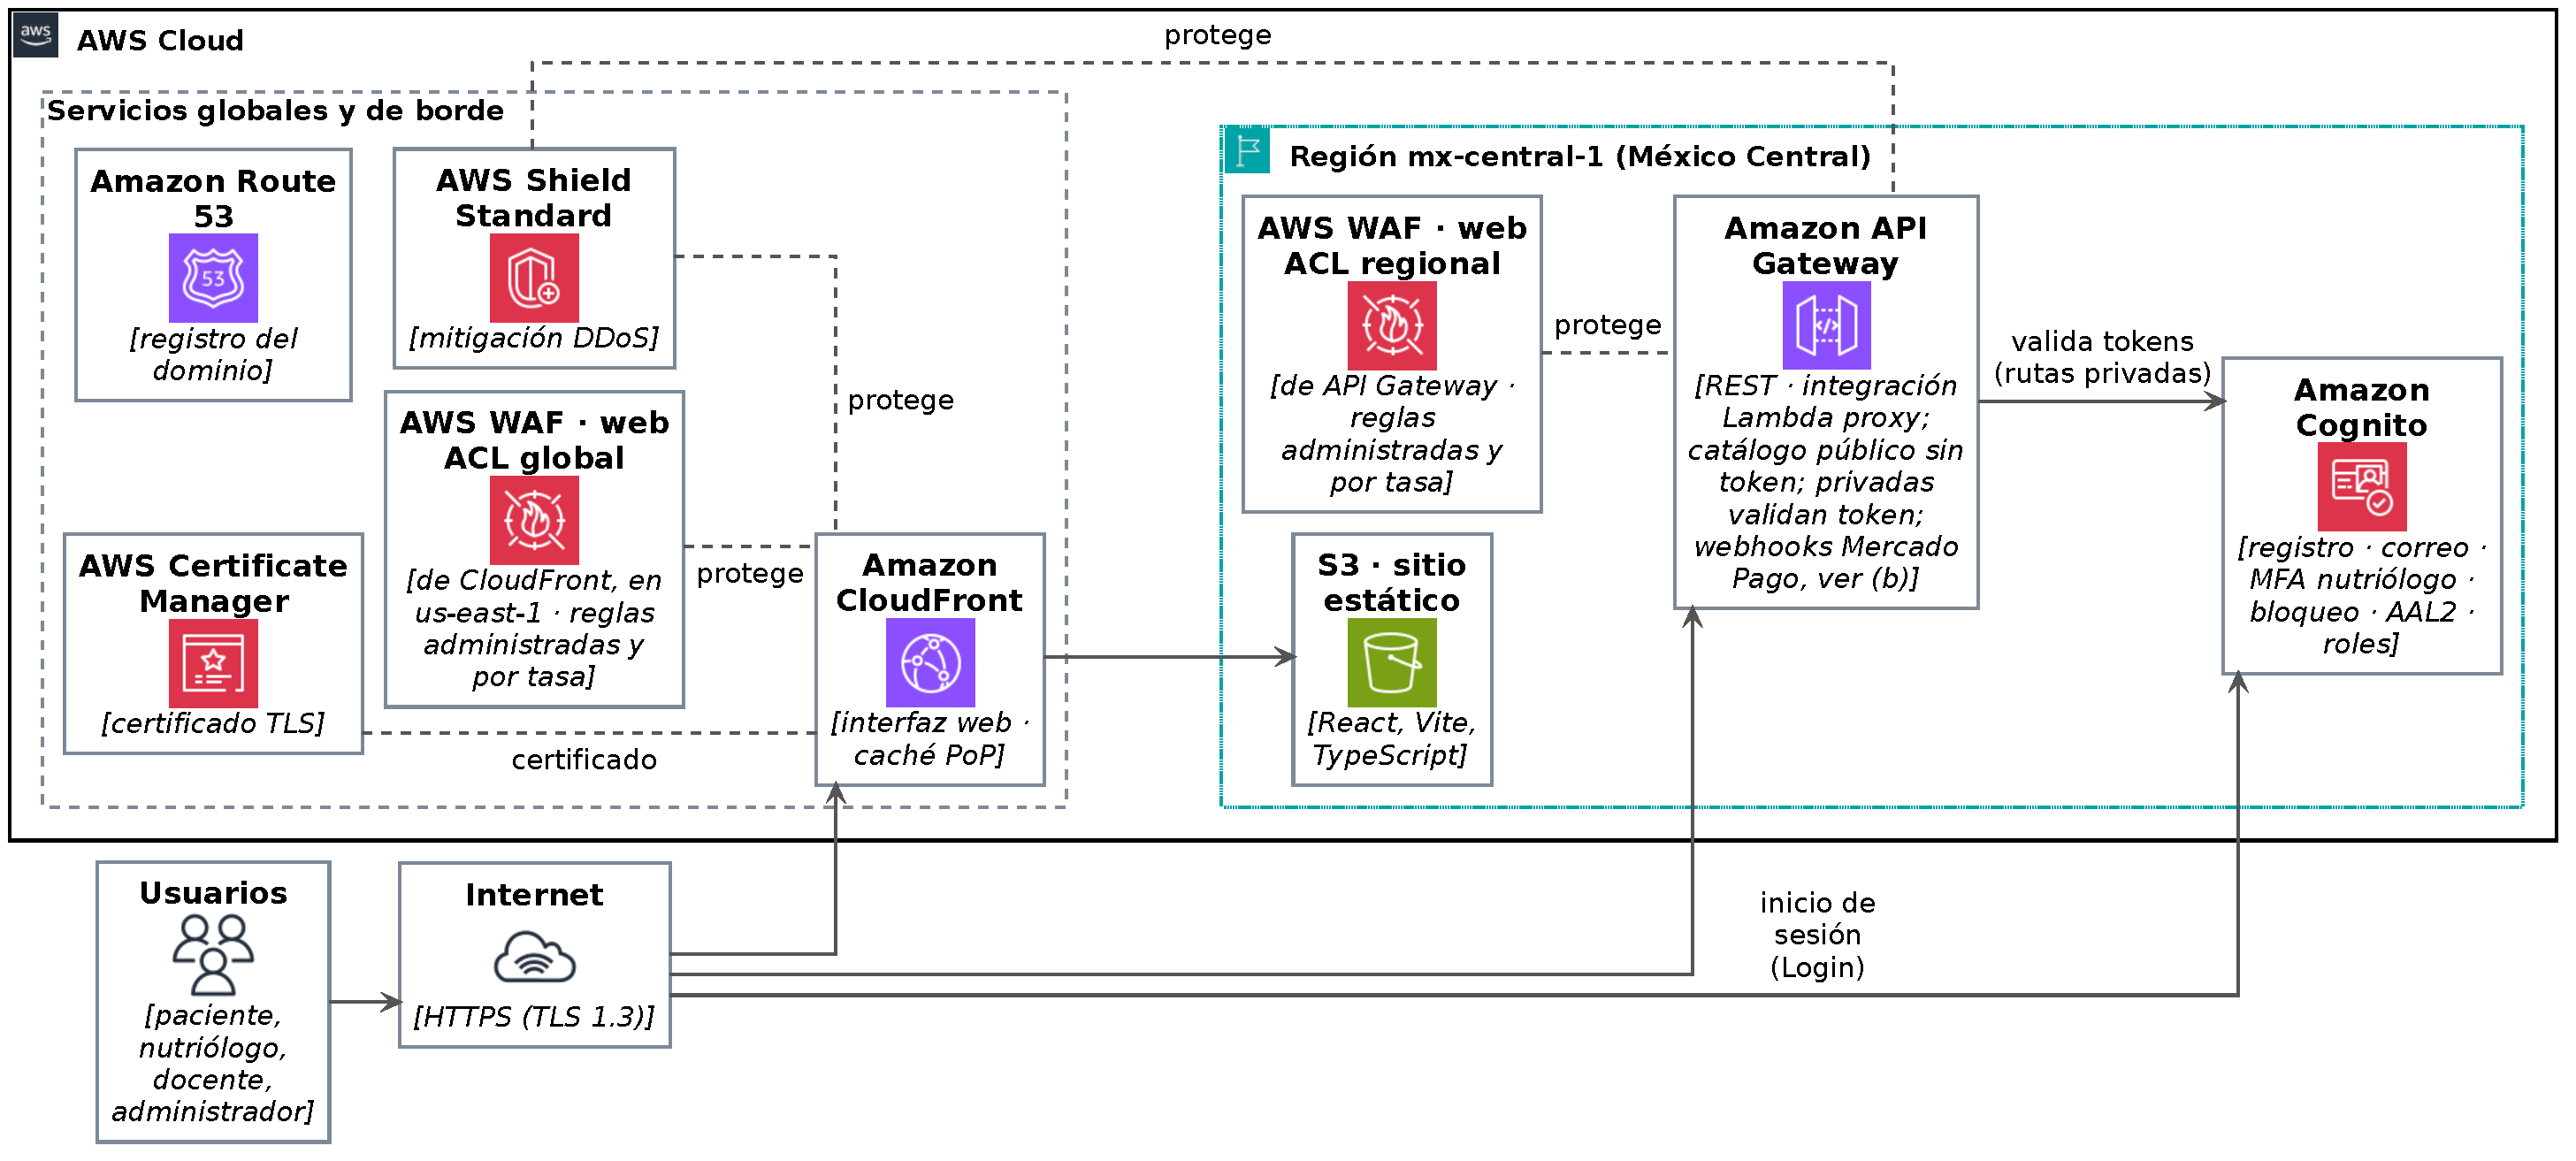
\includegraphics[width=\linewidth,height=0.84\textheight,keepaspectratio]{aws-a.pdf}
    \caption{Borde global, región \texttt{mx-central-1} y entrada de tráfico.}
    \label{fig:aws-a}
  \end{subfigure}
  \caption{Arquitectura de servicios de NutriApp en AWS: (a) borde y
  entrada; (b) red privada y subcontrataciones; (c) almacenamiento y
  llaves; (d) operación y trazabilidad.}
  \label{fig:aws}
\end{figure}
\end{landscape}
 
\begin{figure}[H]
  \ContinuedFloat
  \captionsetup{list=no}
  \centering
  \begin{subfigure}{\linewidth}
    \centering
    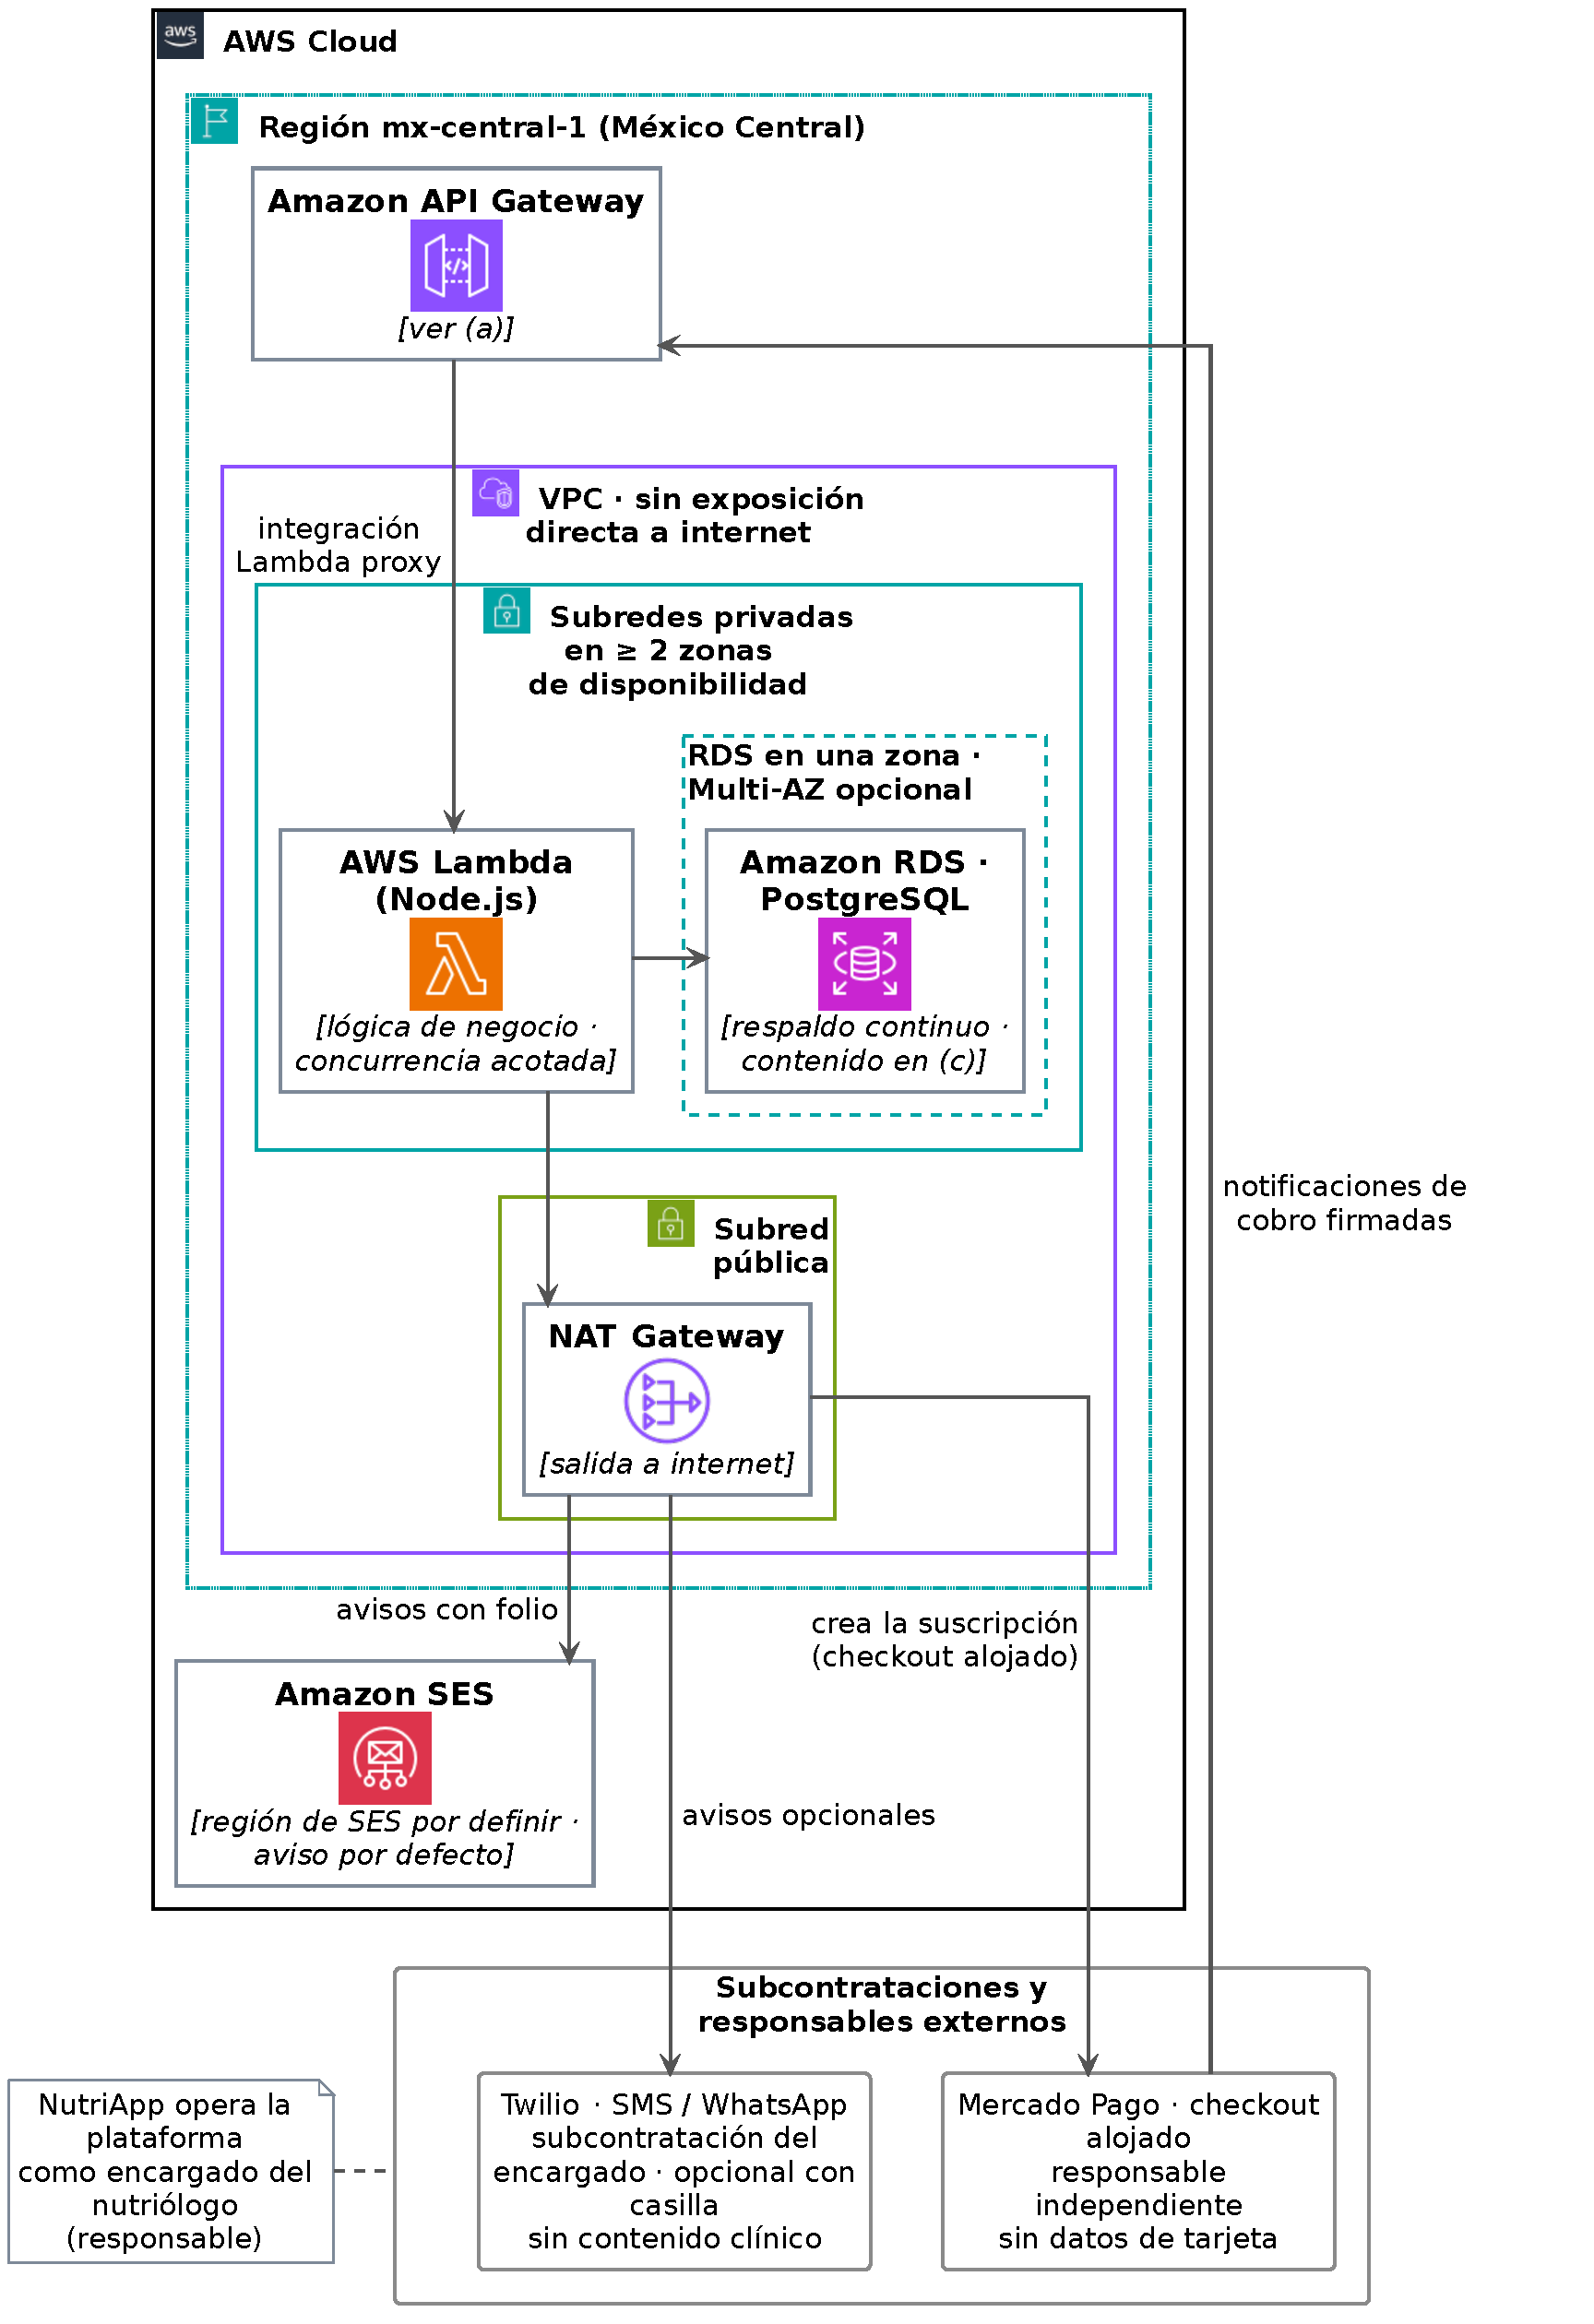
\includegraphics[width=\linewidth,height=0.84\textheight,keepaspectratio]{aws-b.pdf}
    \caption{Red privada, cómputo, salida a internet y subcontrataciones.}
    \label{fig:aws-b}
  \end{subfigure}
  \caption{Arquitectura de servicios de NutriApp en AWS (continuación).}
\end{figure}
 
\begin{figure}[H]
  \ContinuedFloat
  \captionsetup{list=no}
  \centering
  \begin{subfigure}{\linewidth}
    \centering
    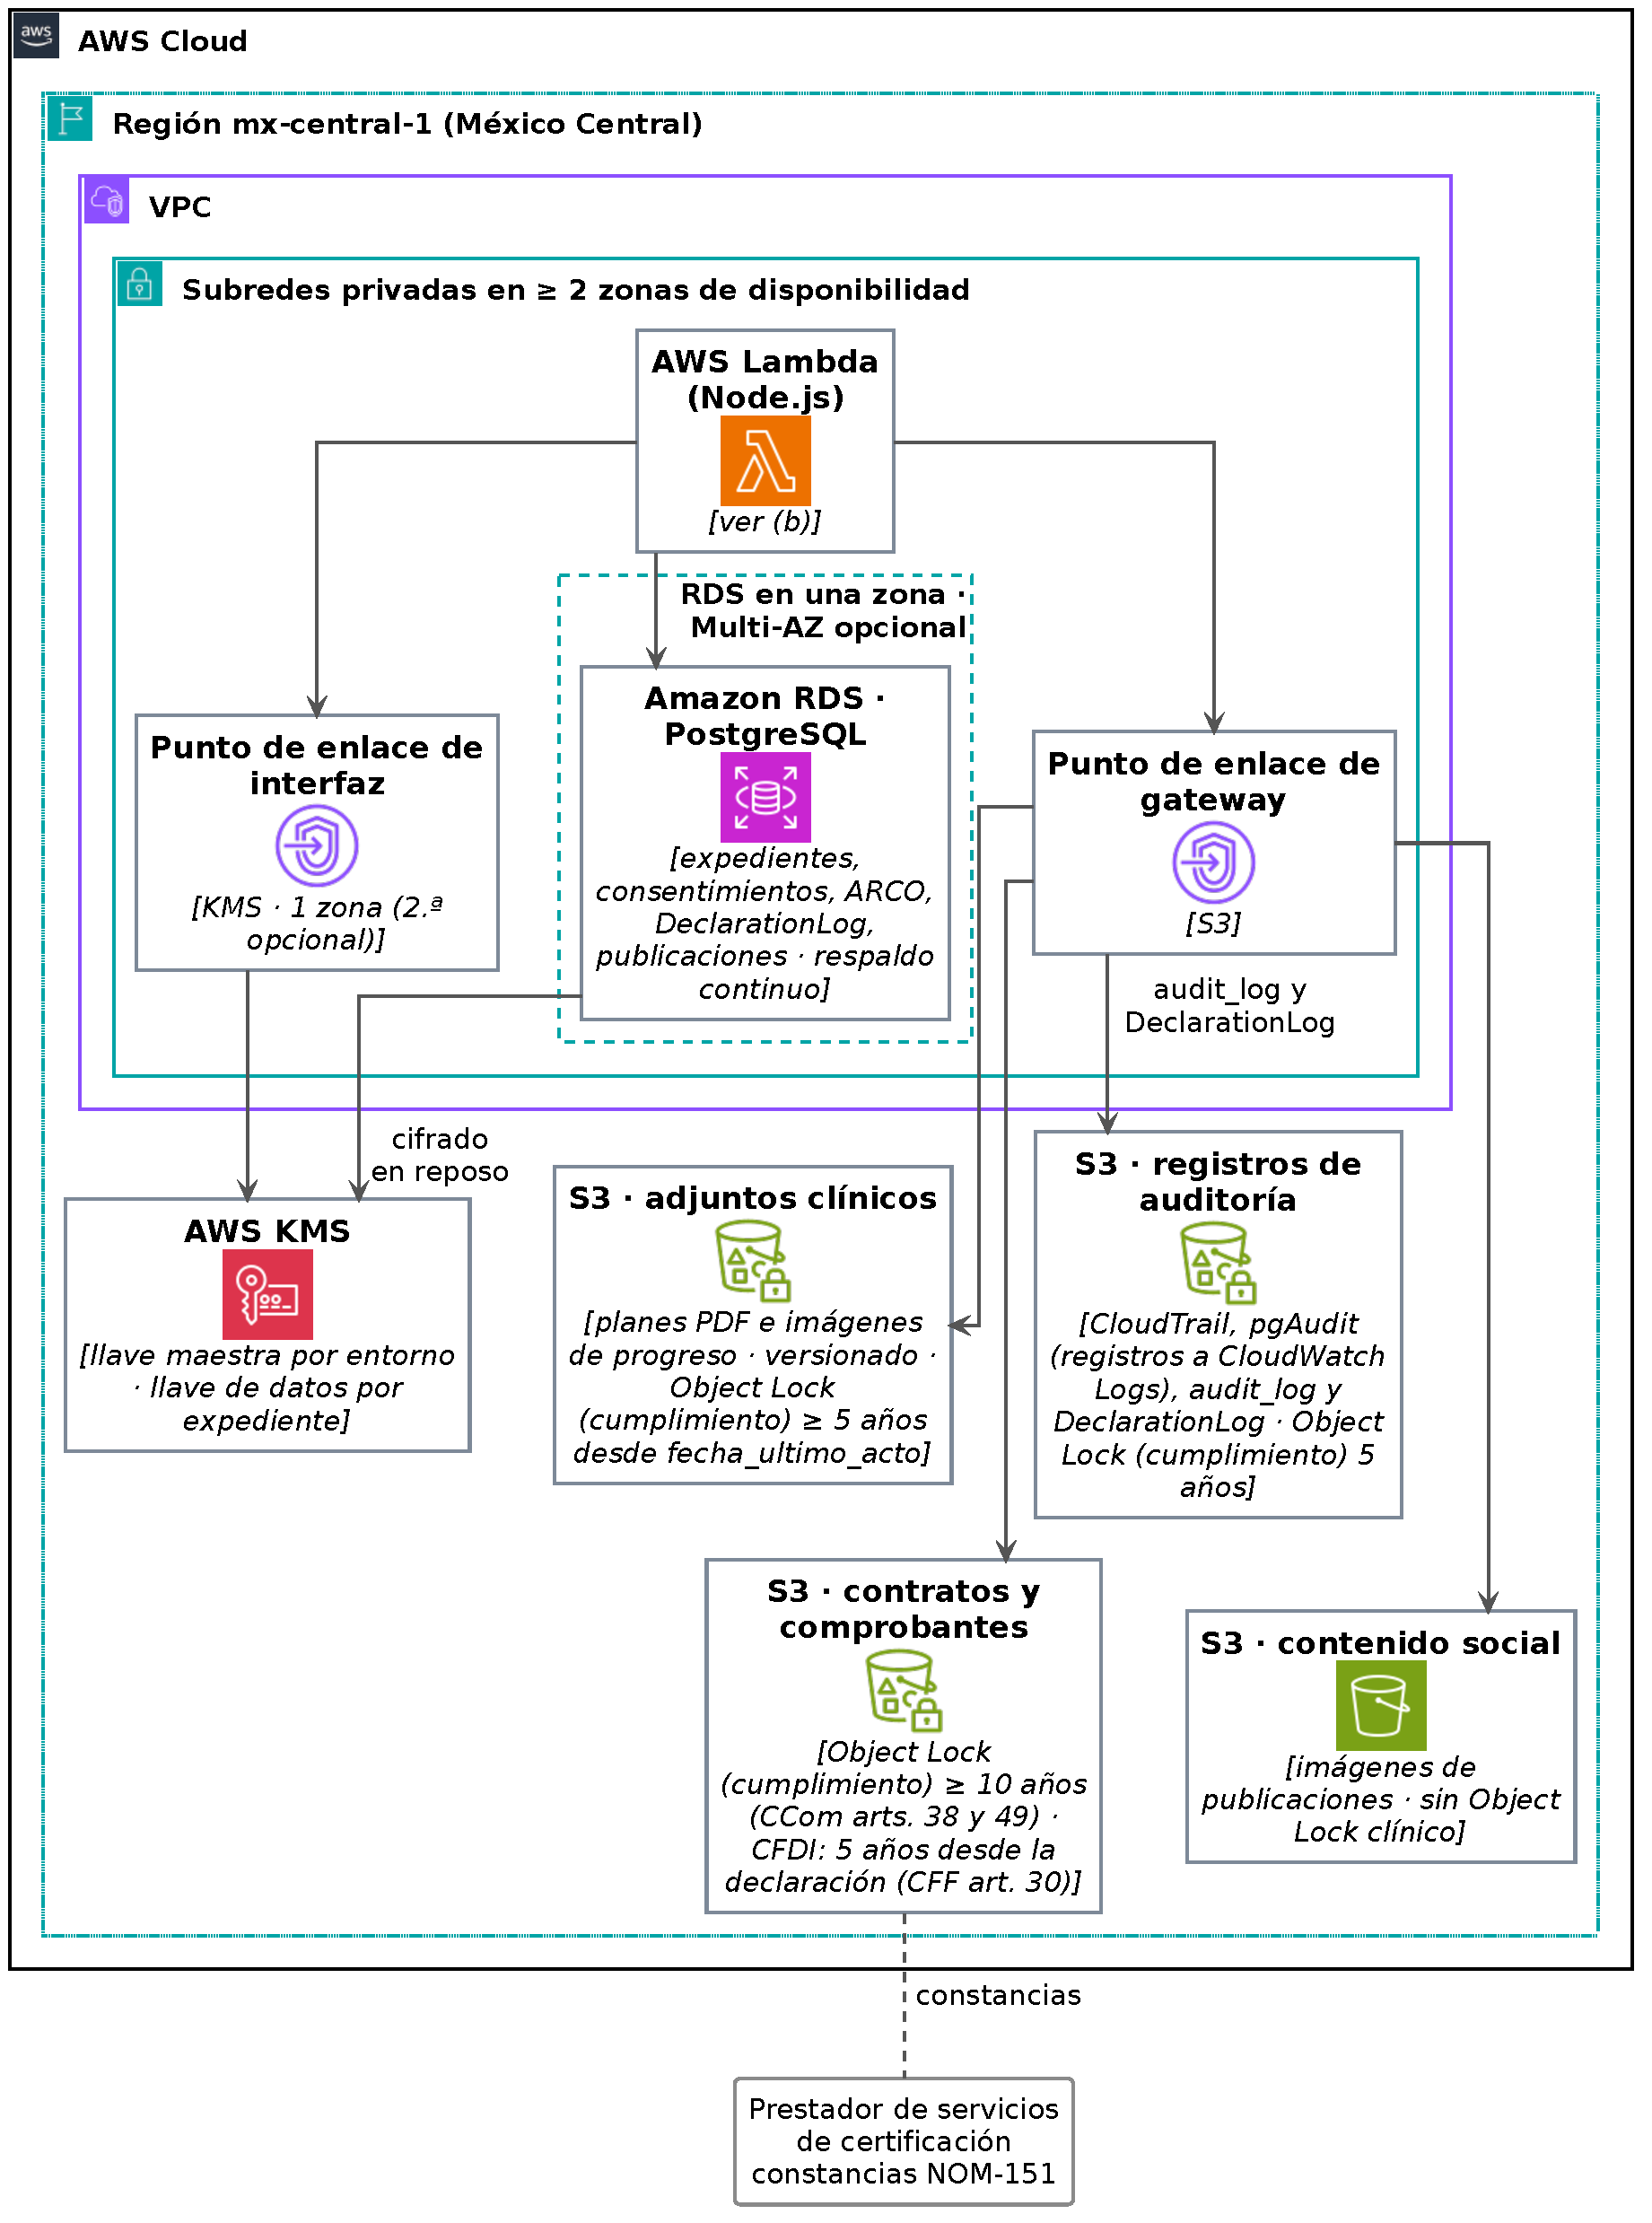
\includegraphics[width=\linewidth,height=0.84\textheight,keepaspectratio]{aws-c.pdf}
    \caption{Almacenamiento, retención y llaves.}
    \label{fig:aws-c}
  \end{subfigure}
  \caption{Arquitectura de servicios de NutriApp en AWS (continuación).}
\end{figure}
 
\begin{figure}[H]
  \ContinuedFloat
  \captionsetup{list=no}
  \centering
  \begin{subfigure}{\linewidth}
    \centering
    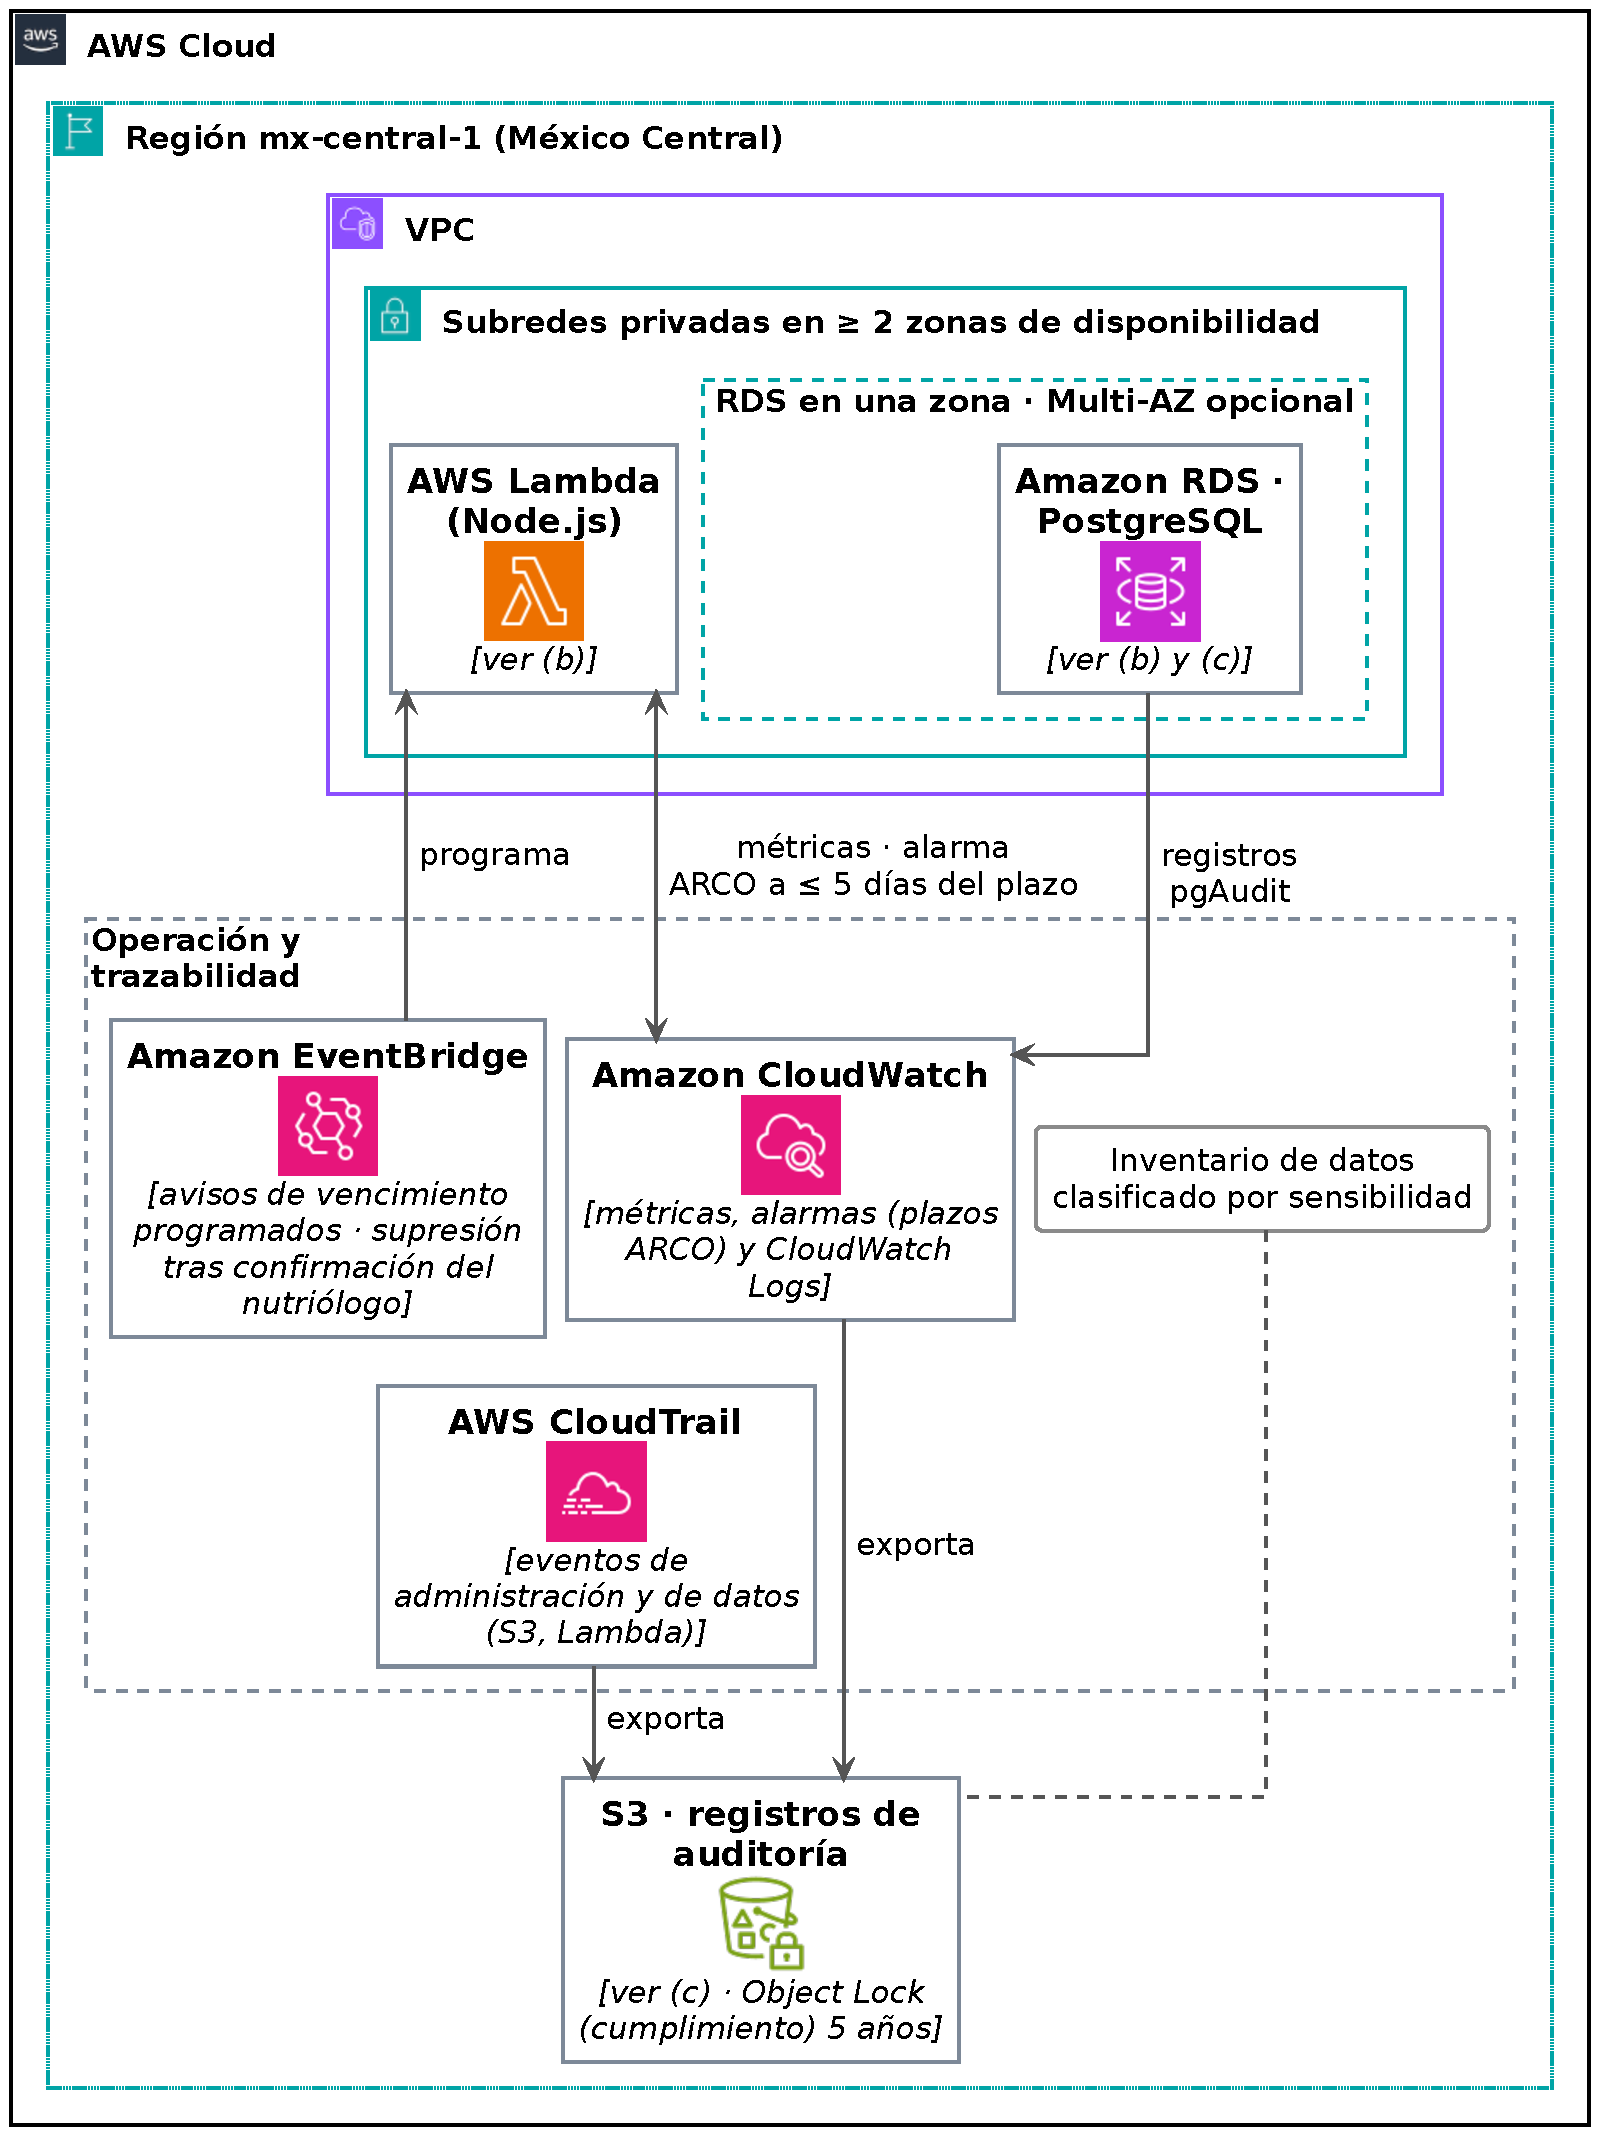
\includegraphics[width=\linewidth,height=0.84\textheight,keepaspectratio]{aws-d.pdf}
    \caption{Operación, métricas y trazabilidad.}
    \label{fig:aws-d}
  \end{subfigure}
  \caption{Arquitectura de servicios de NutriApp en AWS (continuación).}
\end{figure}

\subsubsection{Diagramas UML: casos de uso y secuencia}

Los casos de uso se reparten en las tres partes de la
Figura~\ref{fig:uml-cu}. Los actores son seis: Paciente, Nutriólogo,
Docente, Estudiante, Administrador y Sistema. La parte~(a) reúne la
gestión clínica y los derechos del titular: el alta del paciente queda
pendiente de consentimiento; el consentimiento es afirmativo, con
folio DEC, y se revoca con registro equivalente; el expediente admite
notas con autor, fecha y hora, plan de alimentación y seguimiento; el
paciente consulta su plan, su progreso y quién accedió a su expediente, y presenta solicitudes
ARCO, que el nutriólogo resuelve en veinte días y ejecuta en los
quince siguientes (LFPDPPP, 2025, art.~31), con bloqueo del expediente cuando la
cancelación procede (sección~2.5.5). La revocación del consentimiento
no tiene efectos retroactivos (LFPDPPP, 2025, art.~7): el expediente
deja de admitir datos nuevos y lo registrado sigue bajo la conservación
de la NOM-004 hasta su supresión con confirmación del nutriólogo. Al
vencer la conservación, el Sistema avisa, el nutriólogo confirma y solo
entonces se suprime el expediente por borrado criptográfico, que queda
con folio en el registro de auditoría. La parte~(b) cubre el
catálogo y las citas: el nutriólogo se registra con declaración bajo
protesta y MFA, define su disponibilidad y publica su ficha con la
cédula y la institución declaradas, con la opción de contratar el
Destacado; el paciente busca, reserva con sesión iniciada y recibe la
aceptación o el rechazo en 48 horas, o alternativas si el plazo vence.
La parte~(c) cubre comunidad, administración y cuentas de práctica:
publicación y consulta de contenido educativo, reporte de
publicaciones, moderación con folio MOD y escala de estados, gestión
de la suscripción, alta de instituciones y códigos, activación de la
cuenta Students con código y correo institucional, consulta de
expedientes ficticios en solo lectura y avance de inducción por el
docente, y aviso de vencimiento de la cuenta Students por el Sistema.
La exportación del expediente no aparece: quedó fuera del producto mínimo viable (MVP);
véase la sección~8.3.
 
\begin{landscape}
\begin{figure}[H]
  \centering
  \begin{subfigure}{\linewidth}
    \centering
    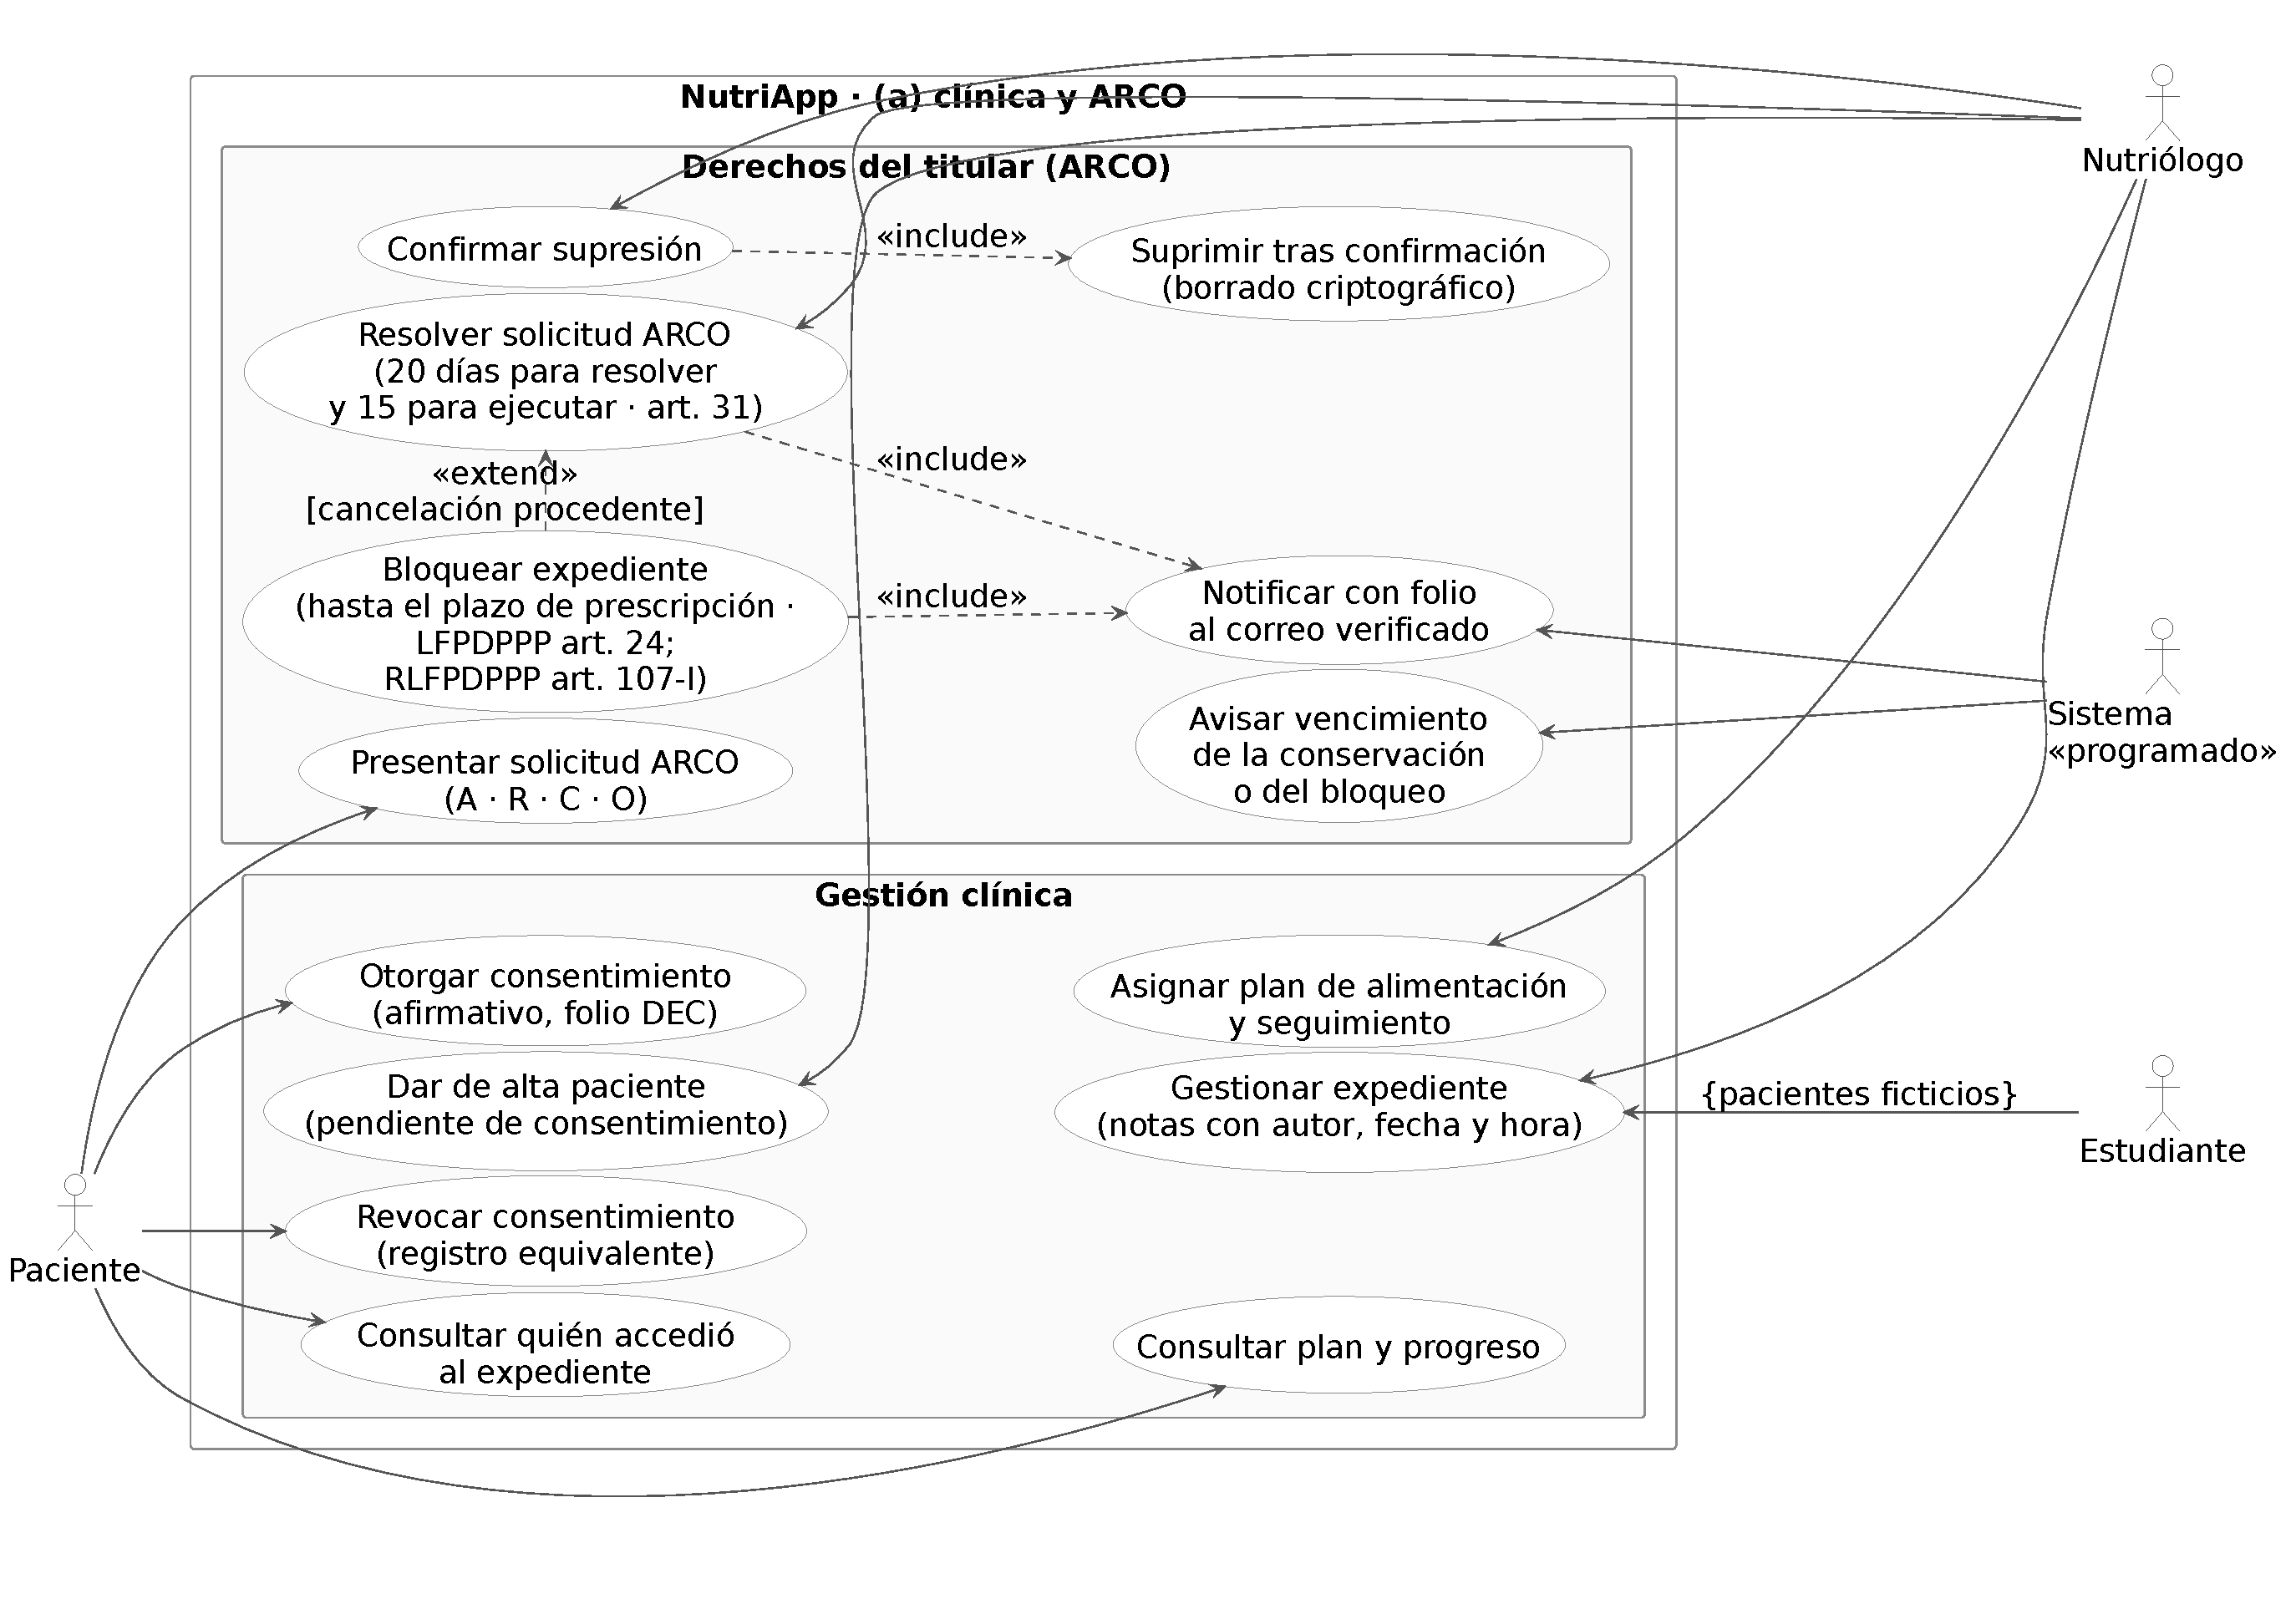
\includegraphics[width=\linewidth,height=0.84\textheight,keepaspectratio]{uml-cu-a.pdf}
    \caption{Gestión clínica y derechos del titular.}
    \label{fig:uml-cu-a}
  \end{subfigure}
  \caption{Casos de uso de NutriApp: (a) clínica y ARCO; (b) catálogo y
  citas; (c) comunidad, administración y cuentas de práctica.}
  \label{fig:uml-cu}
\end{figure}
\end{landscape}
 
\begin{figure}[H]
  \ContinuedFloat
  \captionsetup{list=no}
  \centering
  \begin{subfigure}{\linewidth}
    \centering
    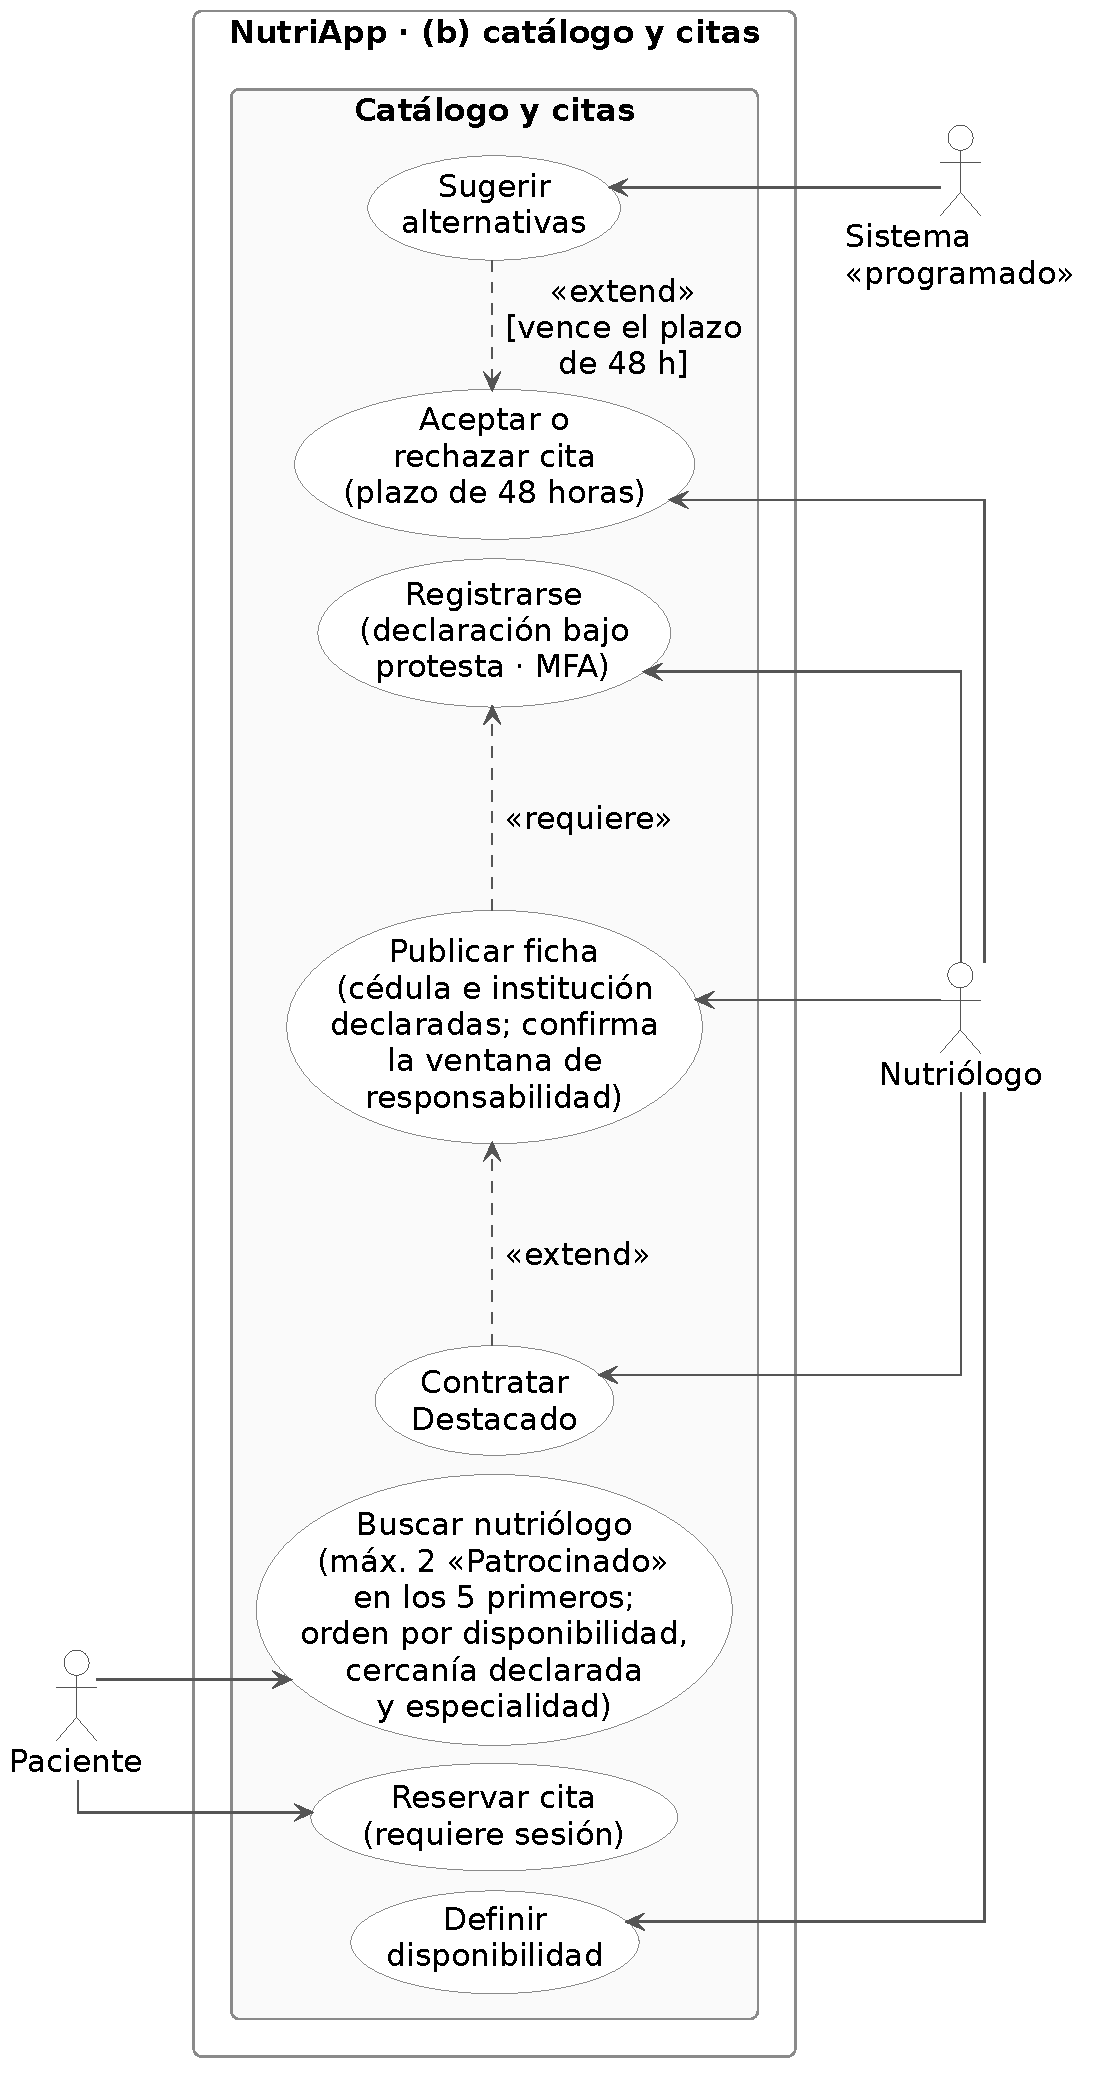
\includegraphics[width=\linewidth,height=0.84\textheight,keepaspectratio]{uml-cu-b.pdf}
    \caption{Catálogo y citas.}
    \label{fig:uml-cu-b}
  \end{subfigure}
  \caption{Casos de uso de NutriApp (continuación).}
\end{figure}
 
\begin{figure}[H]
  \ContinuedFloat
  \captionsetup{list=no}
  \centering
  \begin{subfigure}{\linewidth}
    \centering
    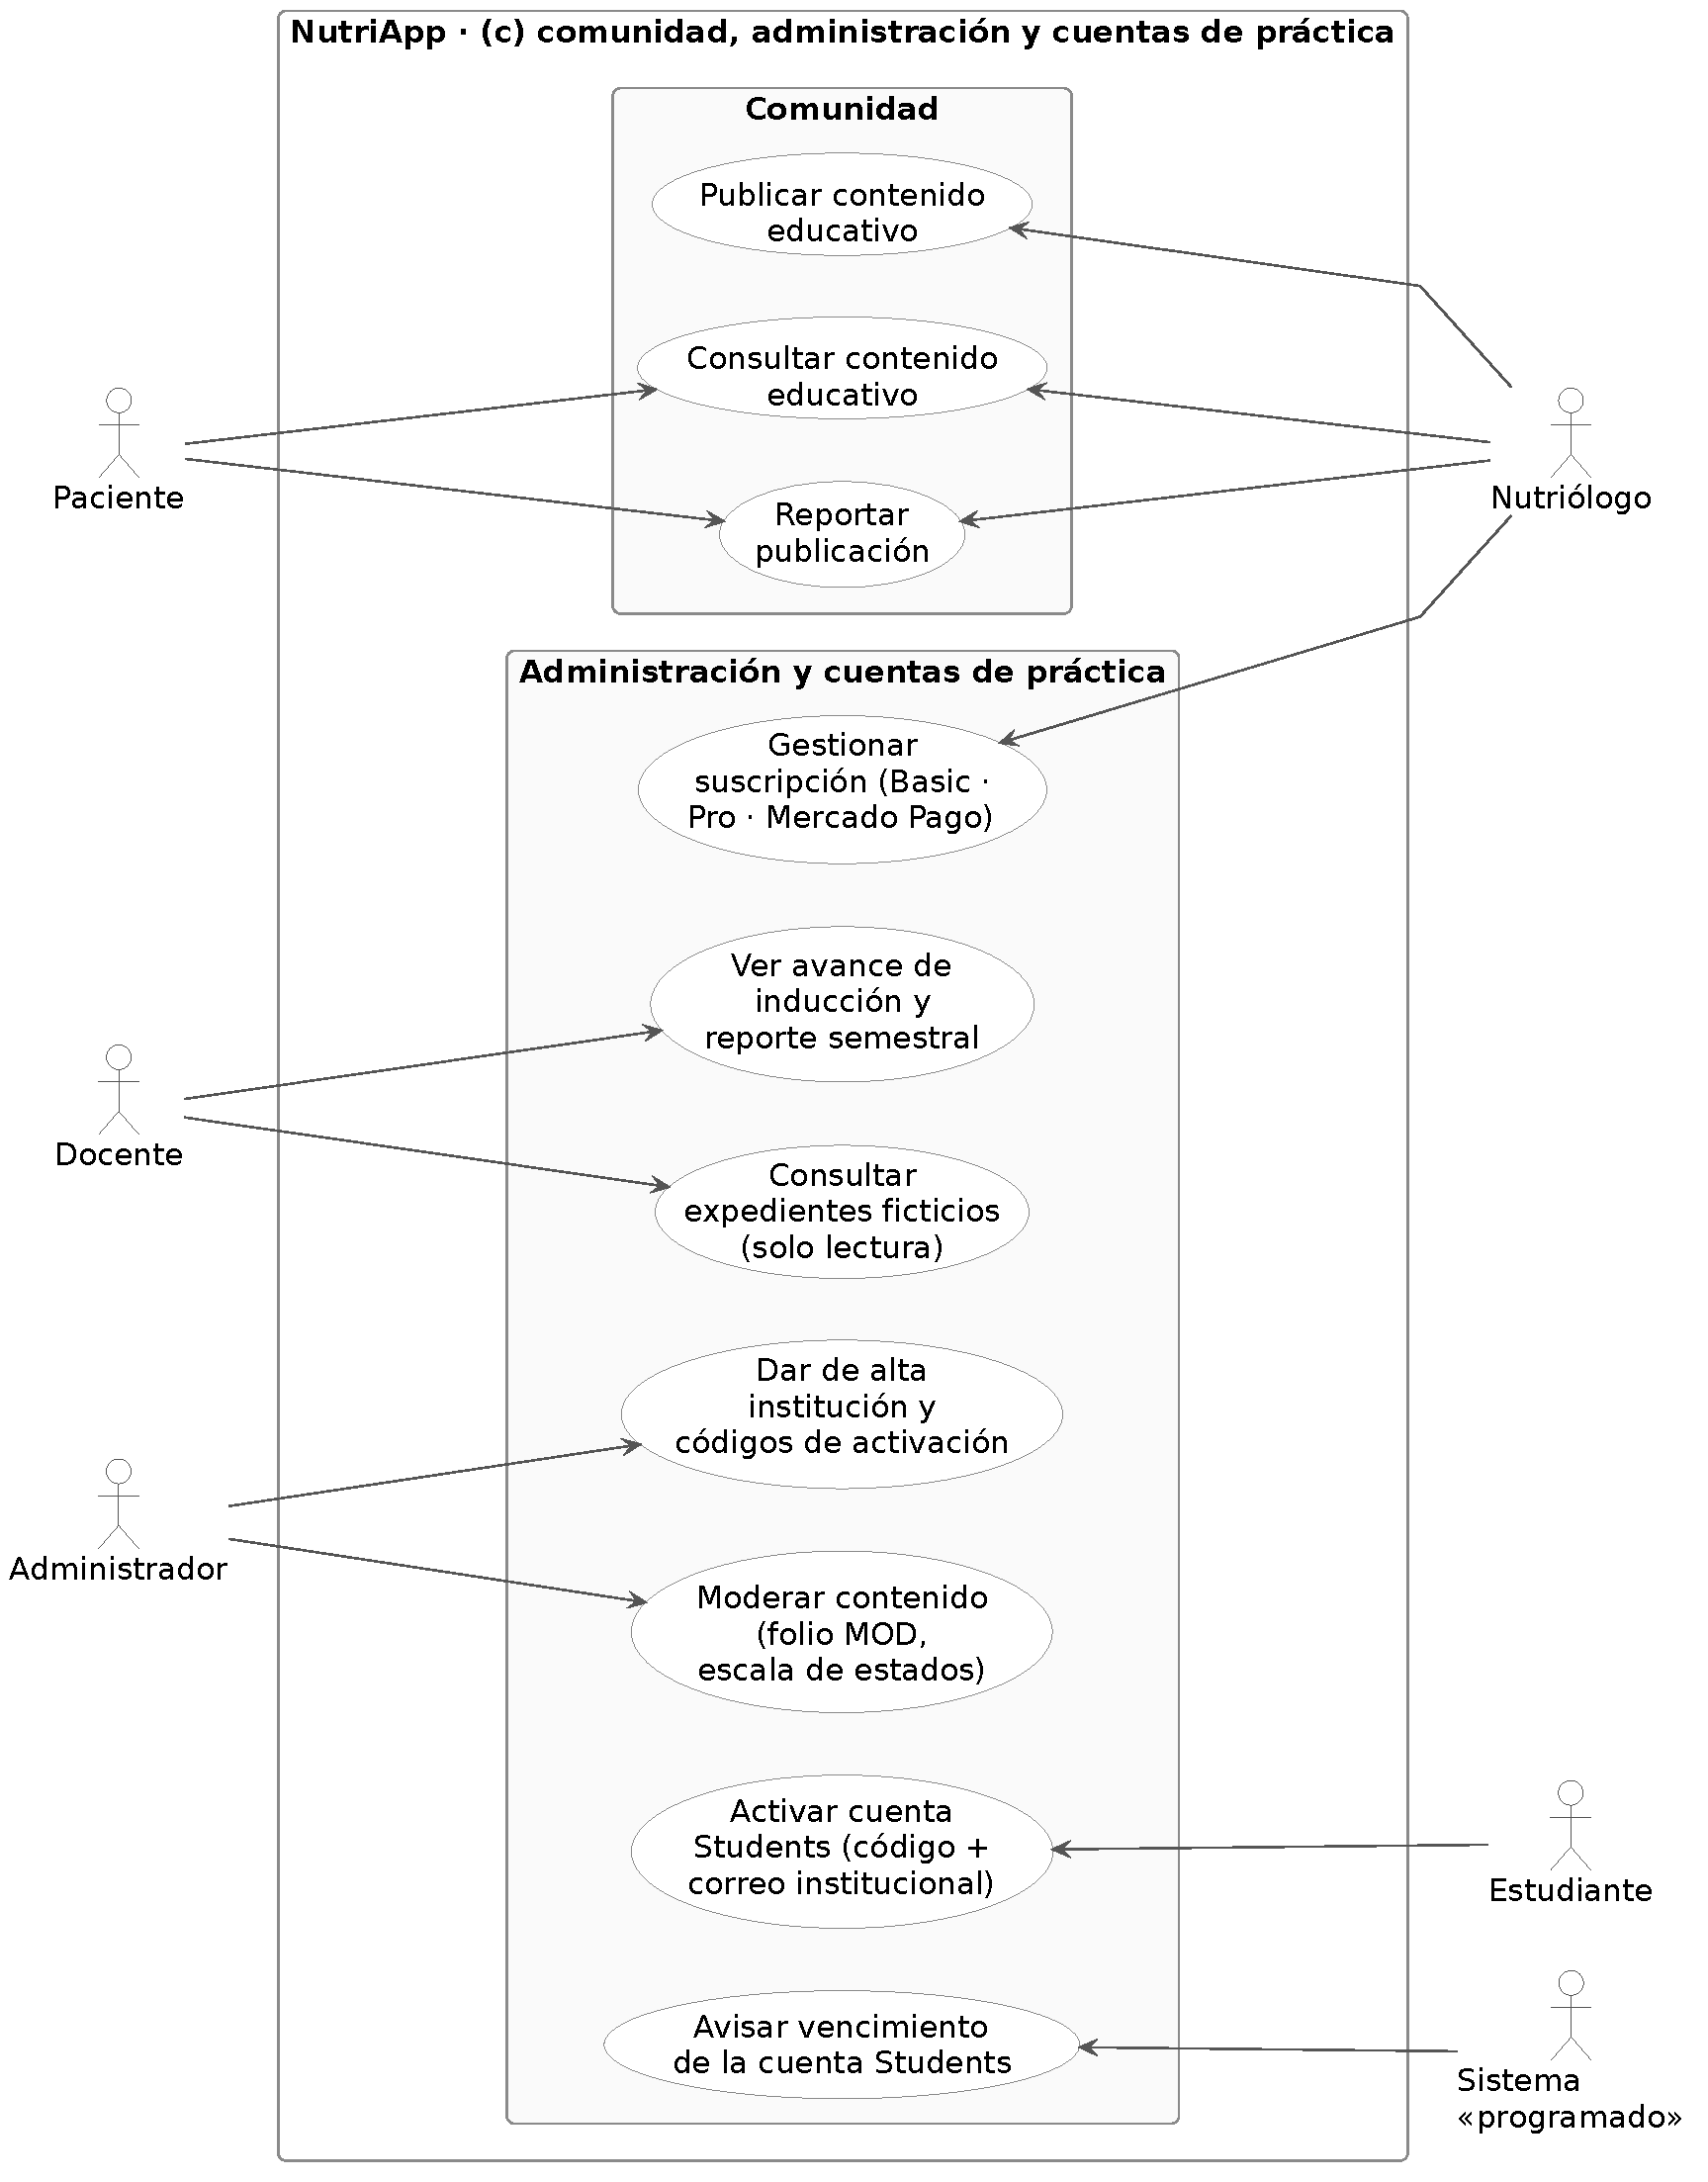
\includegraphics[width=\linewidth,height=0.84\textheight,keepaspectratio]{uml-cu-c.pdf}
    \caption{Comunidad, administración y cuentas de práctica.}
    \label{fig:uml-cu-c}
  \end{subfigure}
  \caption{Casos de uso de NutriApp (continuación).}
\end{figure}
 

El diagrama se lee por actor. El paciente otorga su consentimiento y
presenta las solicitudes ARCO; el nutriólogo las resuelve. Esa
separación es la del responsable y el titular en la ley: el
consentimiento lo da el titular (LFPDPPP, 2025, art.~8) y la respuesta
la debe el responsable en el plazo del artículo~31. El actor Sistema
representa las funciones programadas: el aviso de vencimiento de la
conservación o del bloqueo, la notificación con folio al correo
confirmado, el aviso previo al vencimiento de la cuenta Students y la
sugerencia de alternativas cuando una cita vence sin respuesta. La
supresión no es autónoma: el sistema avisa el vencimiento, el
nutriólogo confirma la supresión y solo entonces se ejecuta el
borrado criptográfico (sección~2.5.5).
El bloqueo resulta de una cancelación que el nutriólogo resuelve
procedente; ninguna función programada lo inicia. Las
relaciones «include» marcan pasos que siempre acompañan al caso que
los incluye, como la notificación con folio que sigue a toda
resolución de una solicitud ARCO; la relación «extend»
marca un paso que solo ocurre bajo una condición, como las
alternativas que se ofrecen si el nutriólogo no contesta. La relación «requiere» indica que publicar la ficha exige haberse registrado. El
estudiante usa el mismo caso de gestión de expediente que el
nutriólogo, acotado a pacientes ficticios; el docente consulta
esos expedientes en modo de lectura y revisa el avance de inducción y el reporte semestral. El administrador modera
contenido y da de alta instituciones y códigos, pero ninguno de sus
casos de uso toca un expediente clínico, en congruencia con el control
de acceso por rol de la sección~2.5.2.

El flujo de reserva de cita, el que más componentes recorre, se sigue
en la Figura~\ref{fig:uml-seq}: el paciente elige una franja horaria disponible del nutriólogo en
\texttt{FindNutritionist}, inicia sesión en \texttt{Login}, con segundo
factor si lo tiene activado, completa la solicitud en \texttt{ConfirmAppointment} y el nutriólogo recibe una
notificación en \texttt{AppointmentsManager} con un plazo de 48 horas para
aceptar o rechazar. Si no responde en ese plazo, el sistema sugiere al
paciente nutriólogos alternativos.

\begin{figure}[H]
  \centering
  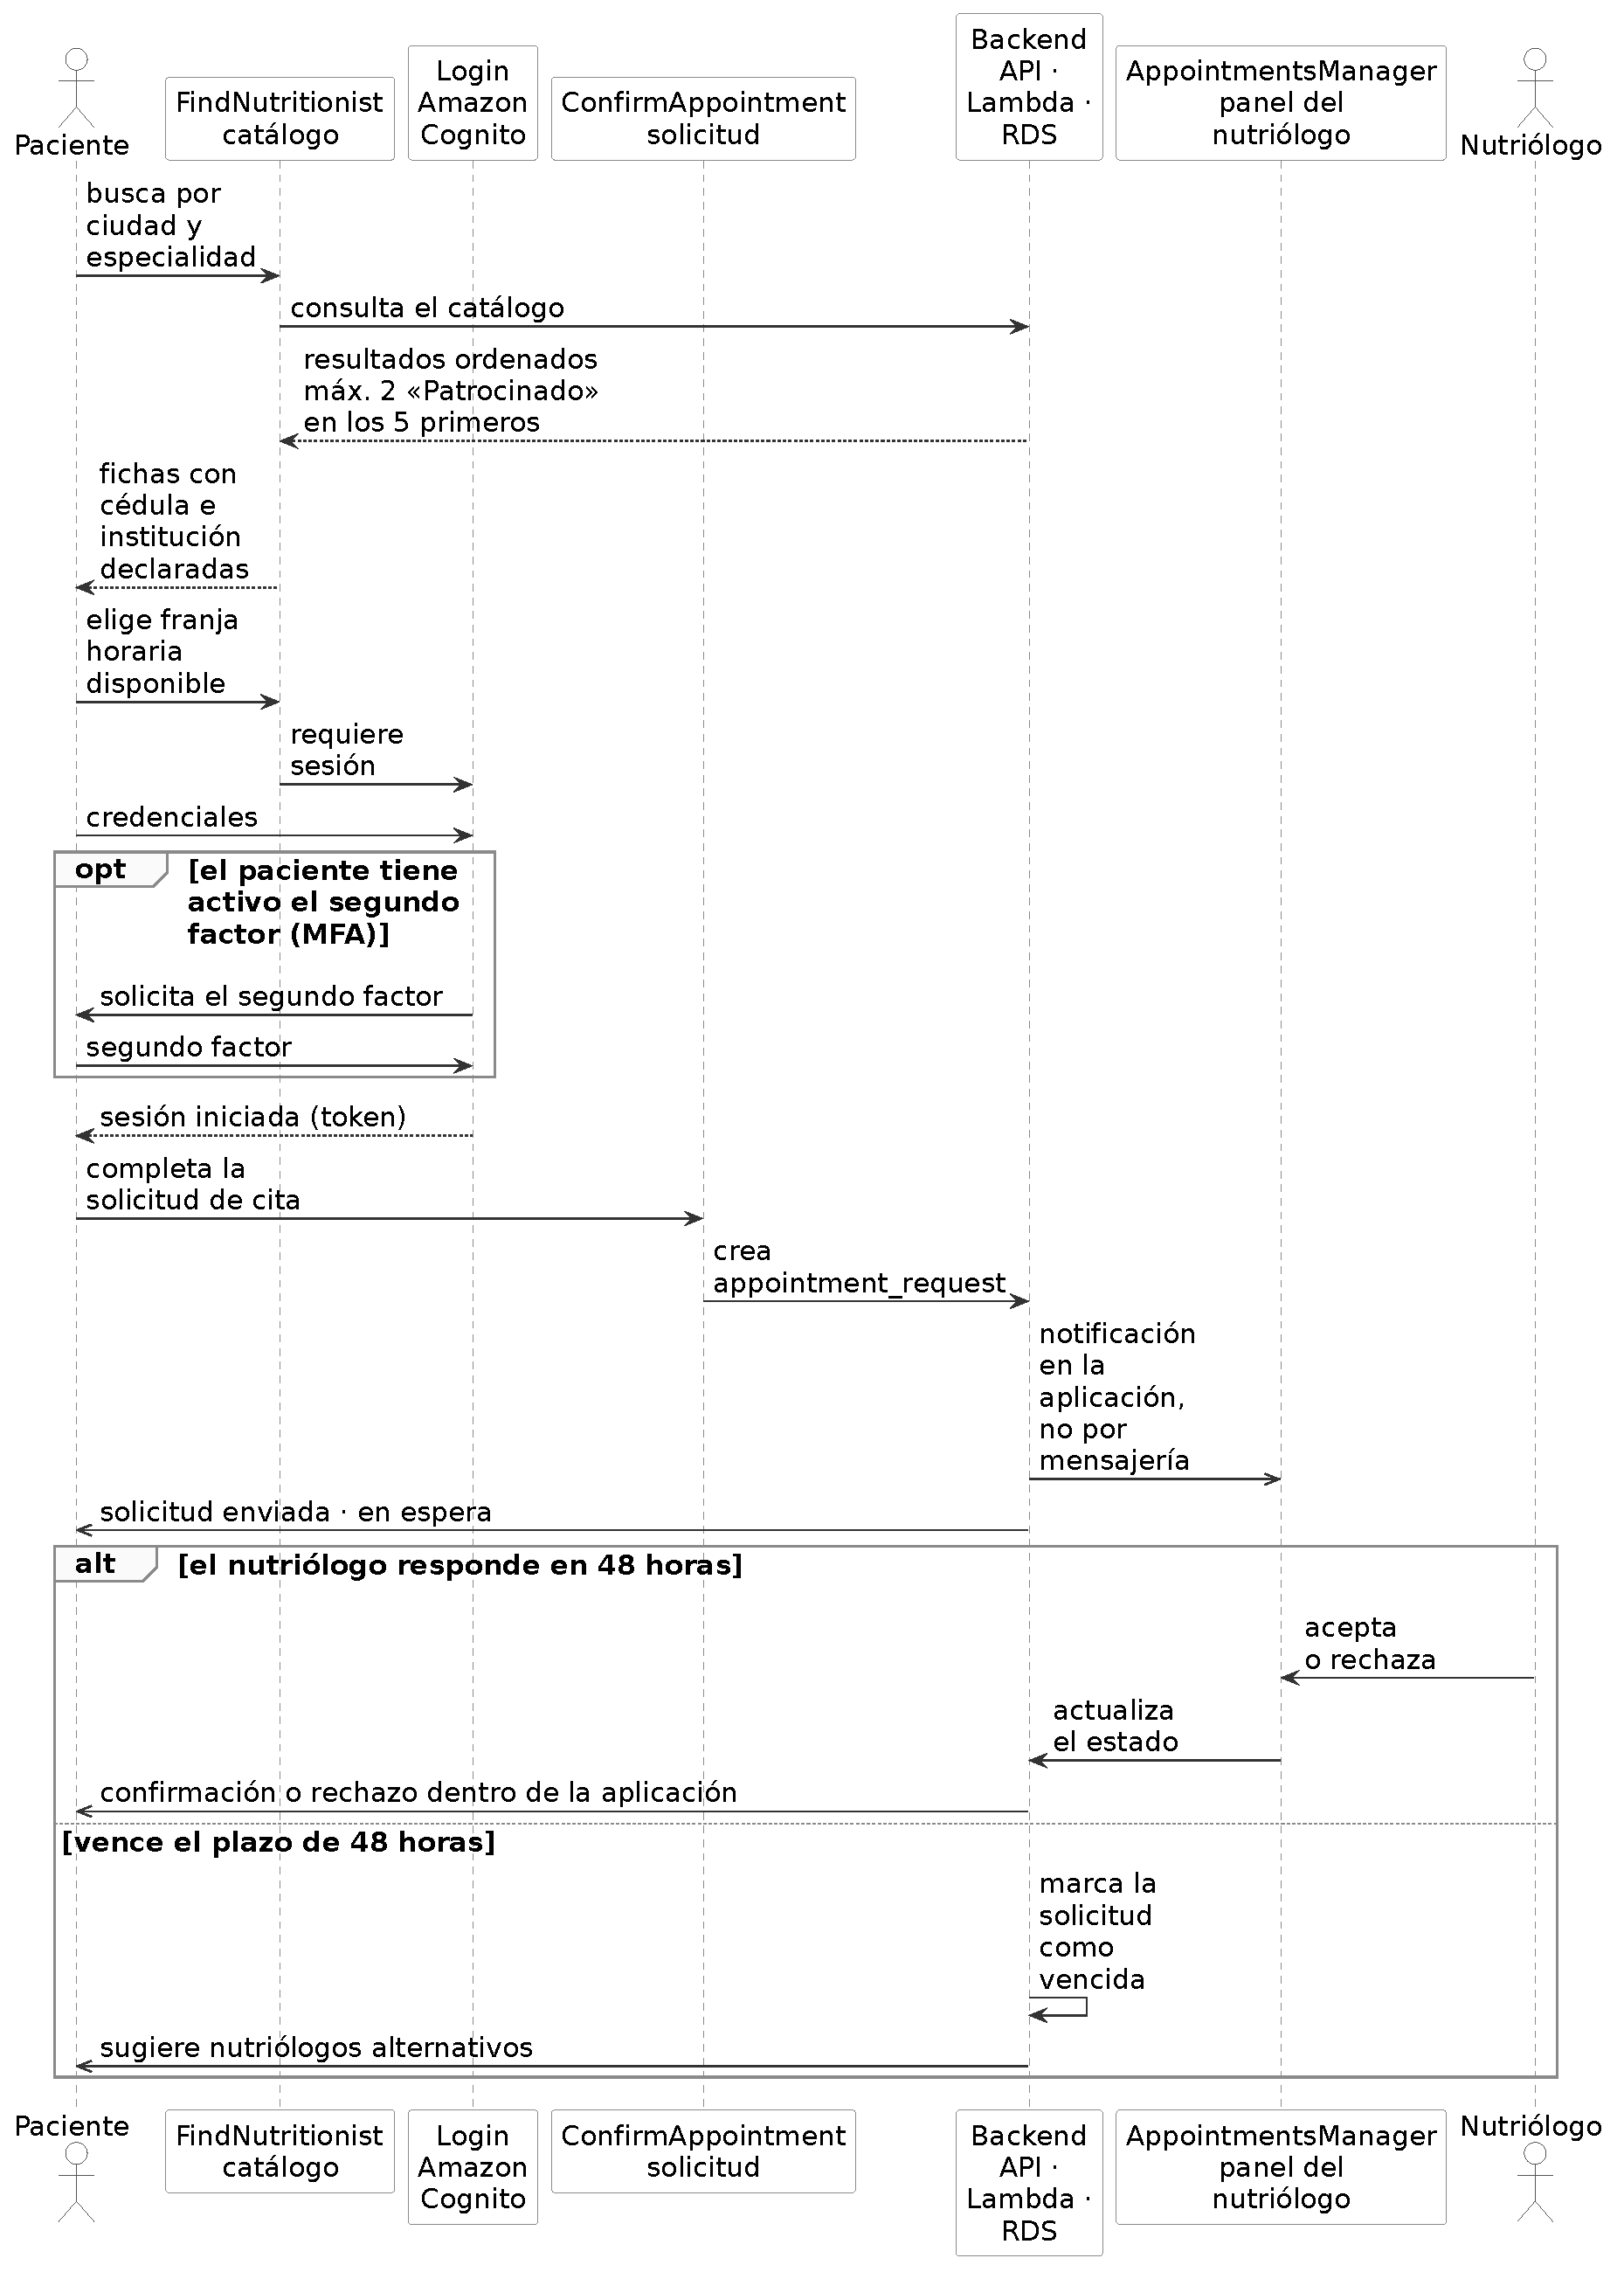
\includegraphics[width=\textwidth]{uml-seq.pdf}
  \caption{Diagrama de secuencia: flujo de reserva de cita y confirmación del
  nutriólogo.}
  \label{fig:uml-seq}
\end{figure}

La secuencia muestra dos decisiones de diseño. La primera es que el
catálogo se consulta sin iniciar sesión: el paciente puede buscar y
comparar fichas sin crear cuenta, y el inicio de sesión solo se pide
cuando elige una franja y va a reservar (con segundo factor si el
paciente lo tiene activado; para el nutriólogo es obligatorio,
sección~2.5.2). La segunda es que la
notificación de la cita viaja dentro de la aplicación y no por
mensajería, conforme a la regla R3 de la sección~7.3 (Tabla~\ref{tab:costos-reglas}); el
nutriólogo la atiende en \texttt{AppointmentsManager}. El bloque
alternativo cierra los dos desenlaces posibles: si el nutriólogo
responde dentro de las 48 horas, el paciente recibe la confirmación o
el rechazo en la aplicación; si el plazo vence, la solicitud se marca
como vencida y el sistema ofrece al paciente otros nutriólogos, sin
que la solicitud quede abierta de forma indefinida.

\subsubsection{Diagrama entidad-relación}

\begin{sloppypar}
El modelo de datos se muestra en la Figura~\ref{fig:er}, en cuatro
partes que corresponden a cuatro bloques de entidades. El bloque
clínico~(a) contiene \texttt{paciente}, \texttt{expediente},
\texttt{plantilla} y \texttt{appointment\_request}, y dentro del expediente
\texttt{plan\_alimentacion}, \texttt{medicion}, \texttt{adjunto} y
\texttt{nota}. El de derechos y trazabilidad~(b) contiene el
\texttt{consentimiento}, la solicitud \texttt{arco\_request}, el
\texttt{incidente} con su tabla asociativa
\texttt{incidente\_expediente}, el \texttt{audit\_log} y el
\texttt{declaration\_log} (la tabla del \texttt{DeclarationLog}). El de cuentas de
práctica, catálogo y suscripción~(c) contiene \texttt{nutriologo},
\texttt{disponibilidad}, \texttt{institution},
\texttt{activation\_code}, \texttt{teacher}, \texttt{featured\_listing},
\texttt{plan\_subscription}, \texttt{contrato\_suscripcion} y
\texttt{pago}. El de comunidad y administración~(d) contiene
\texttt{post}, \texttt{content\_report}, \texttt{moderation\_event} y
\texttt{administrador}. El modelo es relacional y se define en
PostgreSQL sobre Amazon RDS, conforme a la capa de datos de la
sección~5.1.
\end{sloppypar}
 
\begin{landscape}
\begin{figure}[H]
  \centering
  \begin{subfigure}{\linewidth}
    \centering
    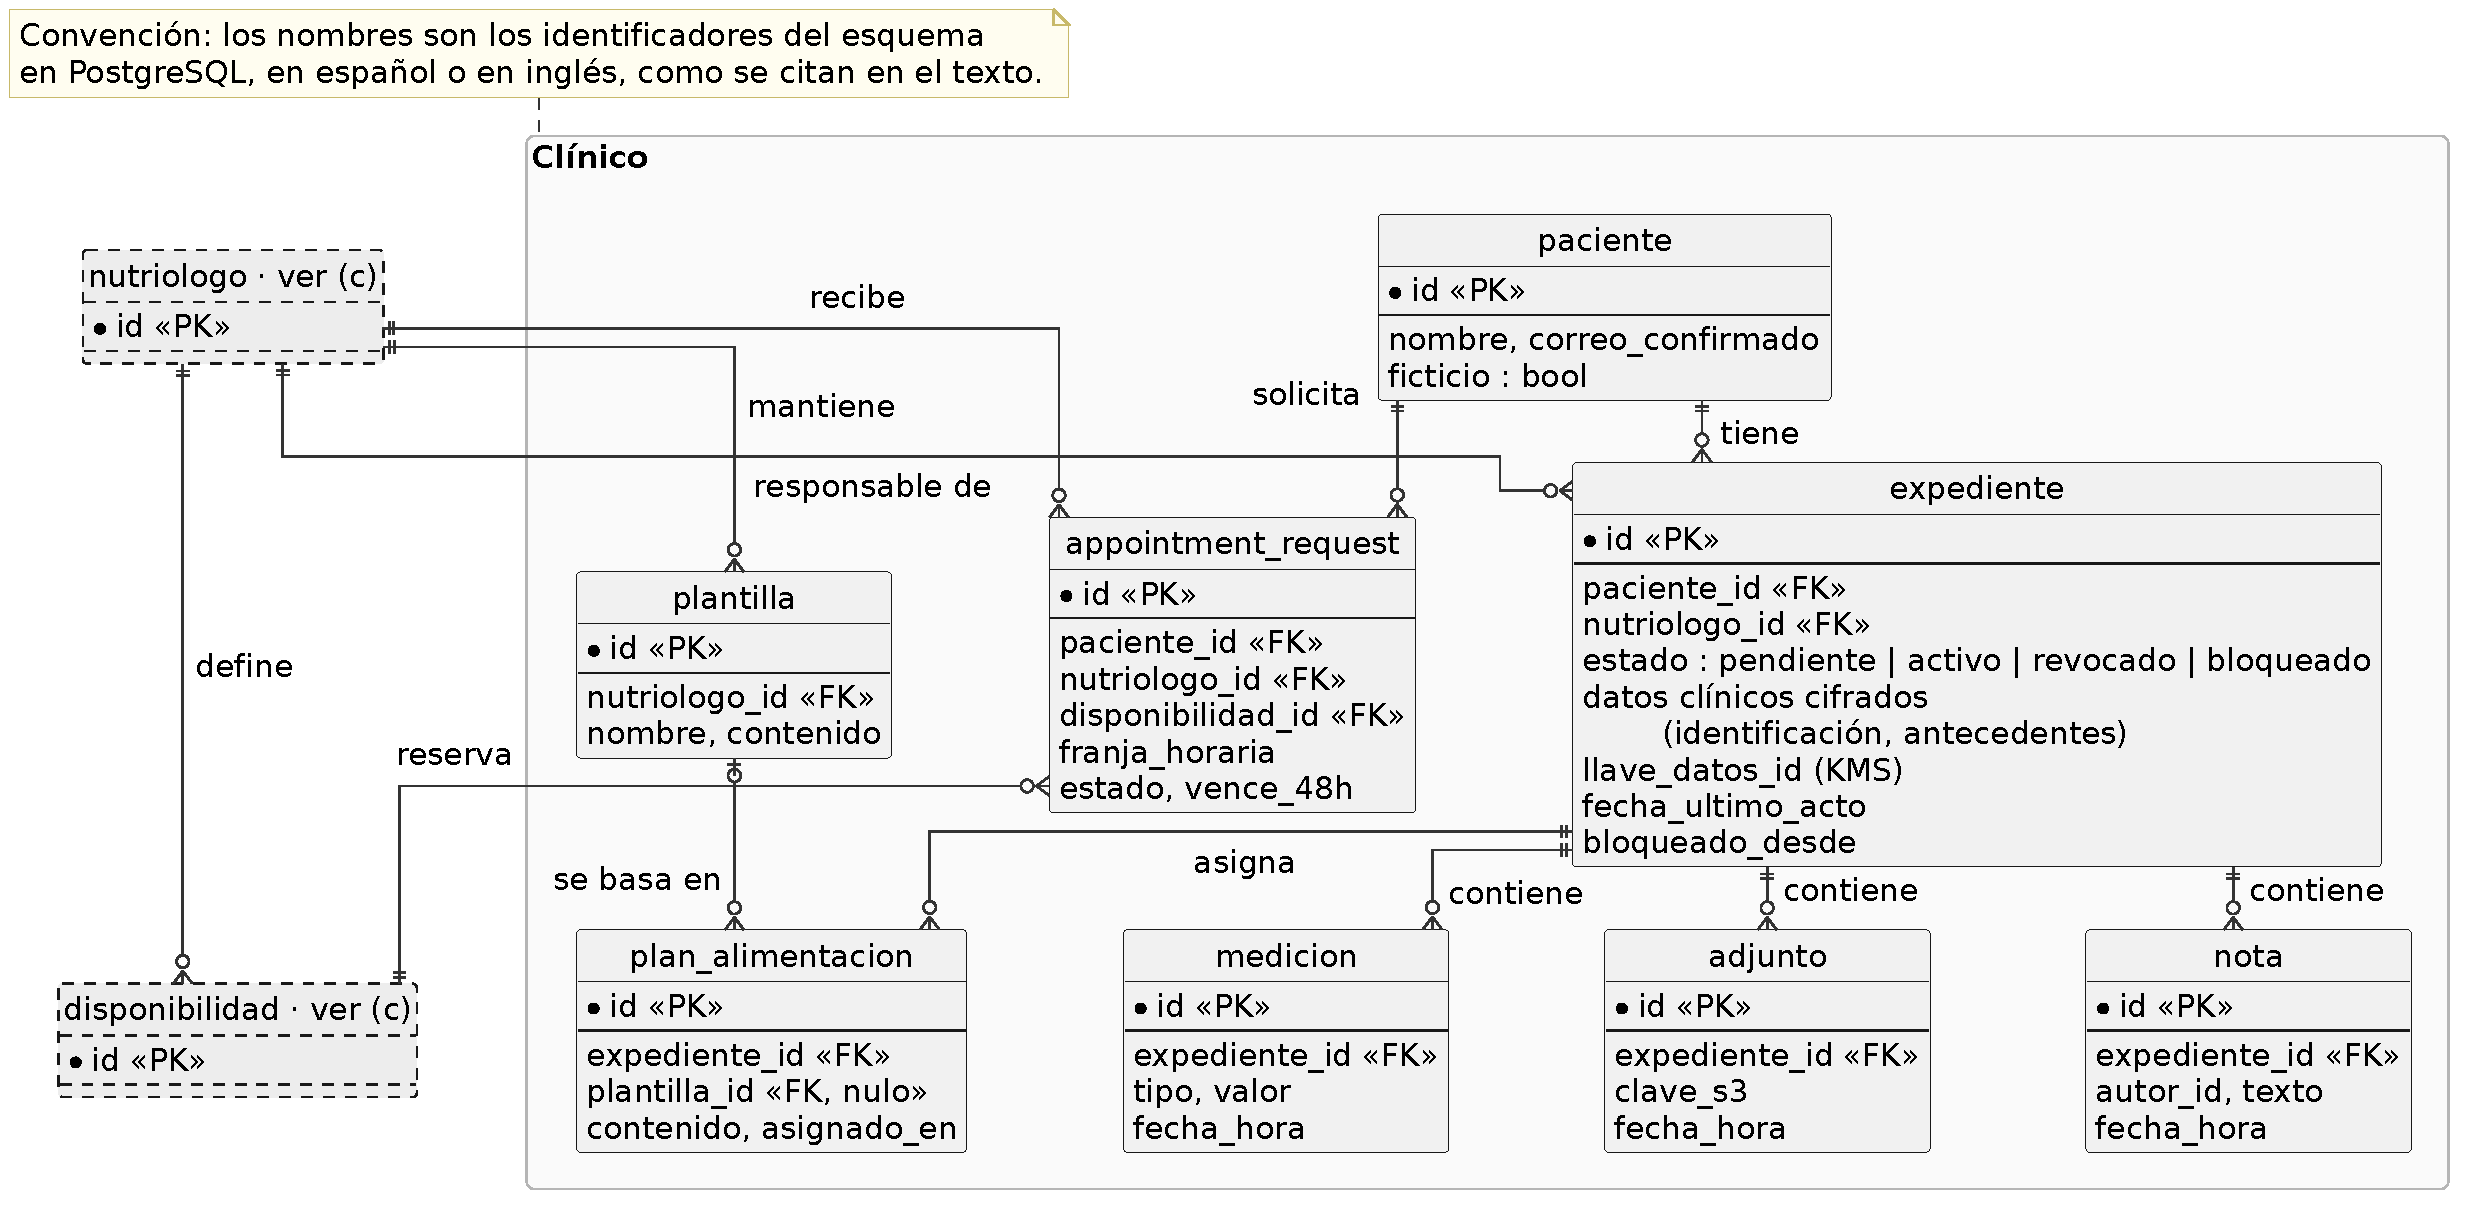
\includegraphics[width=\linewidth,height=0.84\textheight,keepaspectratio]{er-a.pdf}
    \caption{Bloque clínico.}
    \label{fig:er-a}
  \end{subfigure}
  \caption{Modelo entidad-relación de NutriApp: (a) clínico; (b) derechos
  y trazabilidad; (c) cuentas de práctica, catálogo y suscripción;
  (d) comunidad y administración.}
  \label{fig:er}
\end{figure}
\end{landscape}
 
\begin{landscape}
\begin{figure}[H]
  \ContinuedFloat
  \captionsetup{list=no}
  \centering
  \begin{subfigure}{\linewidth}
    \centering
    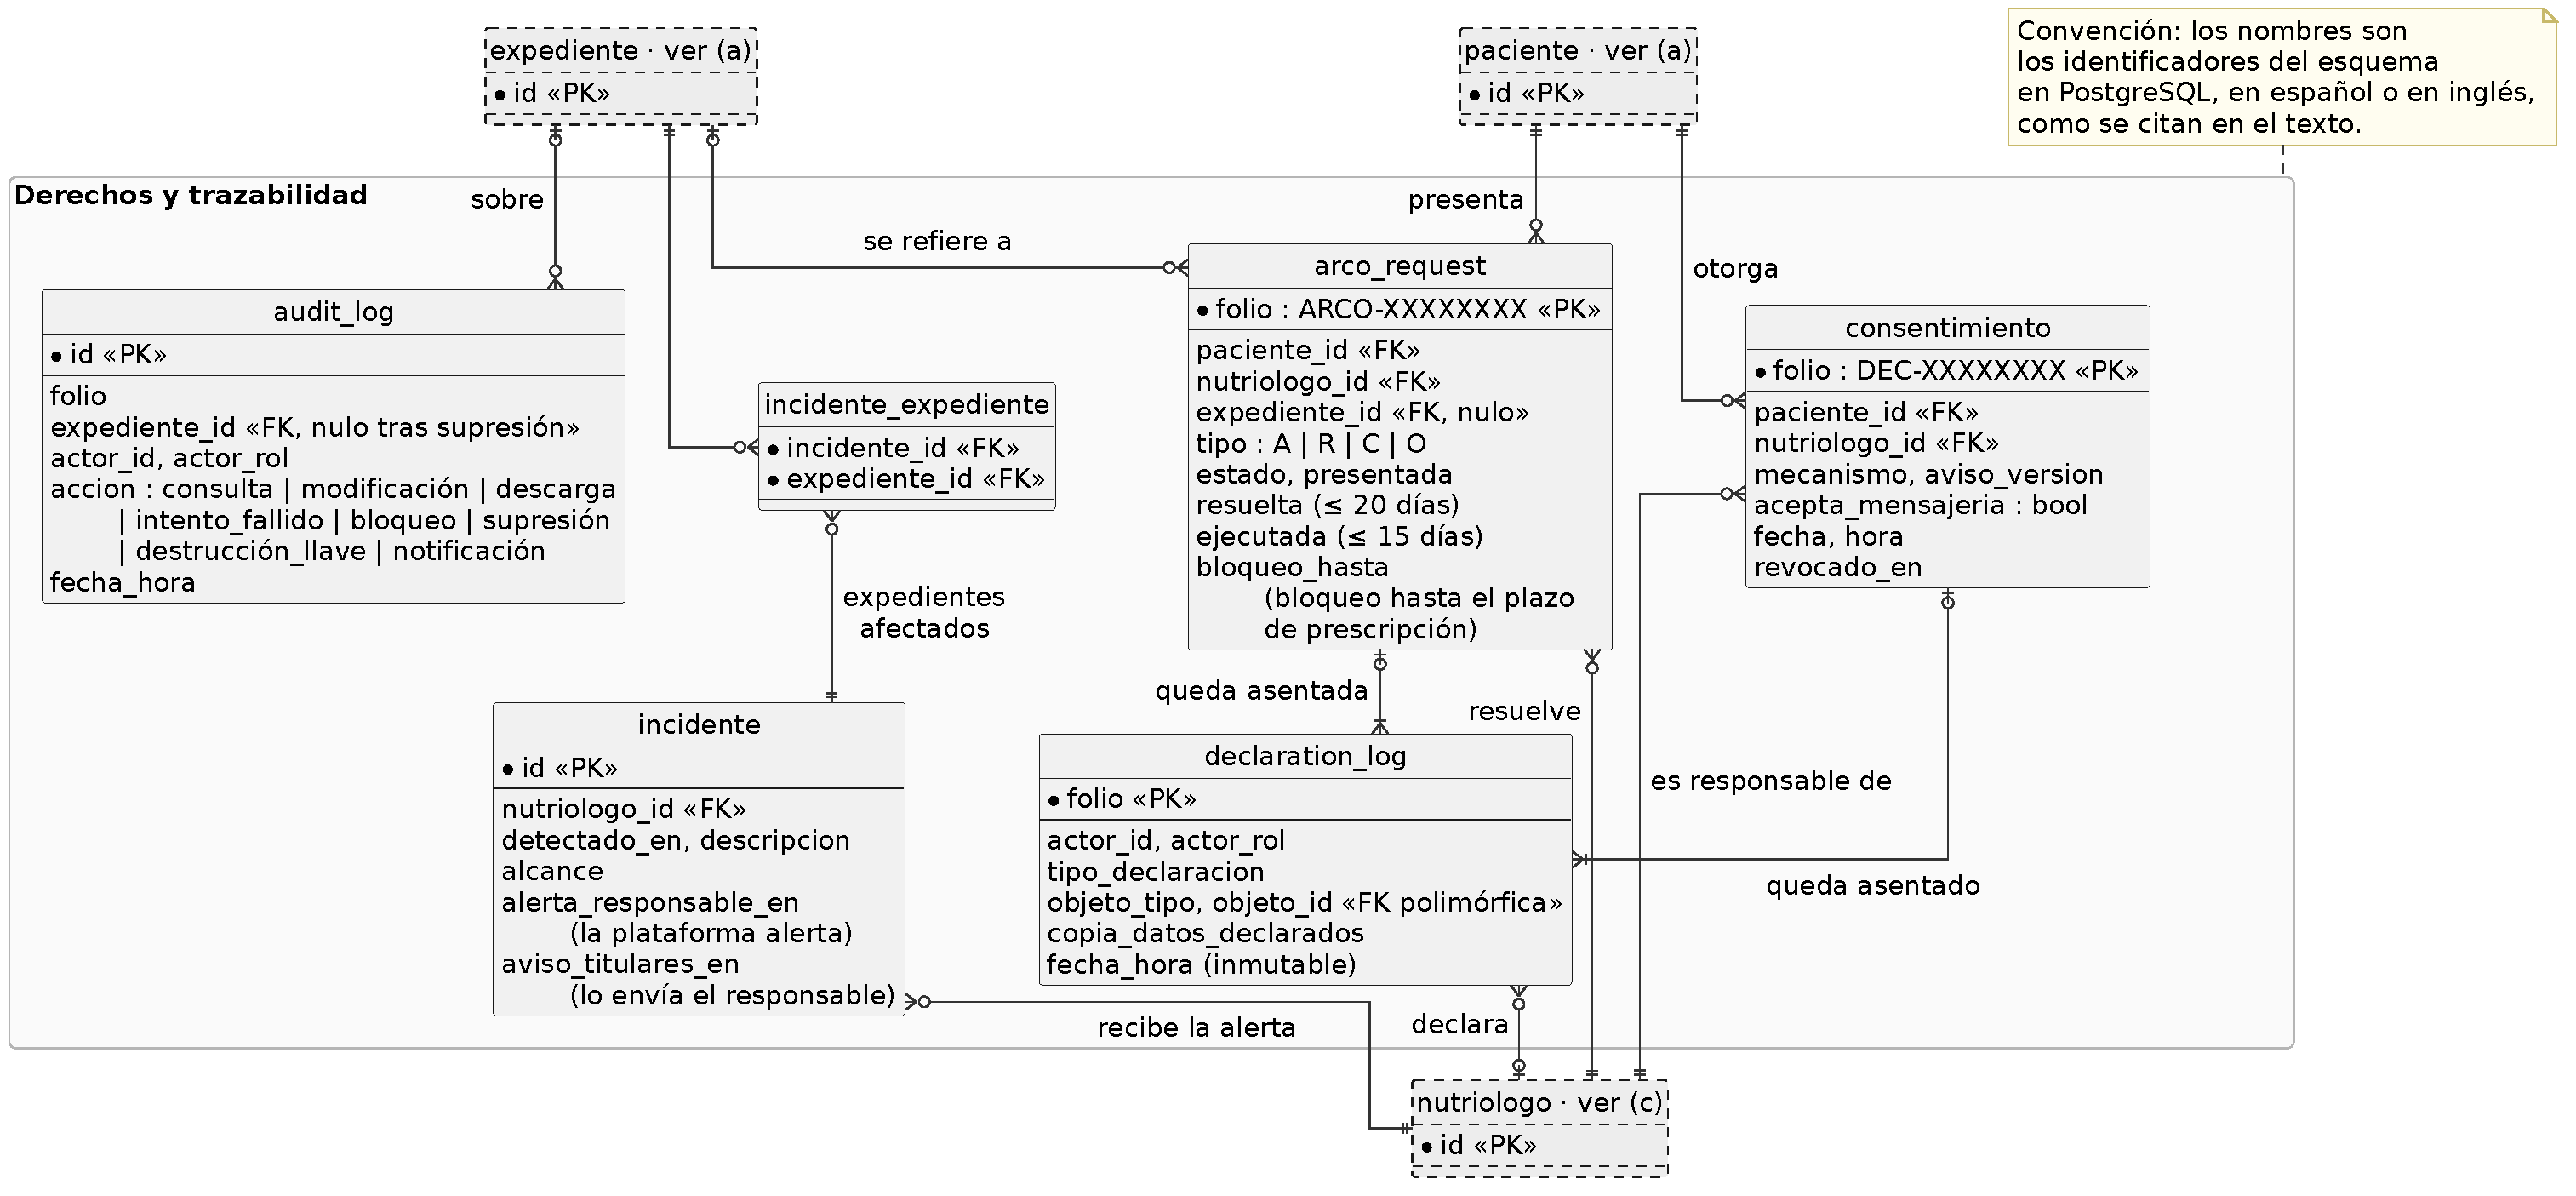
\includegraphics[width=\linewidth,height=0.84\textheight,keepaspectratio]{er-b.pdf}
    \caption{Derechos del titular y trazabilidad.}
    \label{fig:er-b}
  \end{subfigure}
  \caption{Modelo entidad-relación de NutriApp (continuación).}
\end{figure}
\end{landscape}
 
\begin{figure}[H]
  \ContinuedFloat
  \captionsetup{list=no}
  \centering
  \begin{subfigure}{\linewidth}
    \centering
    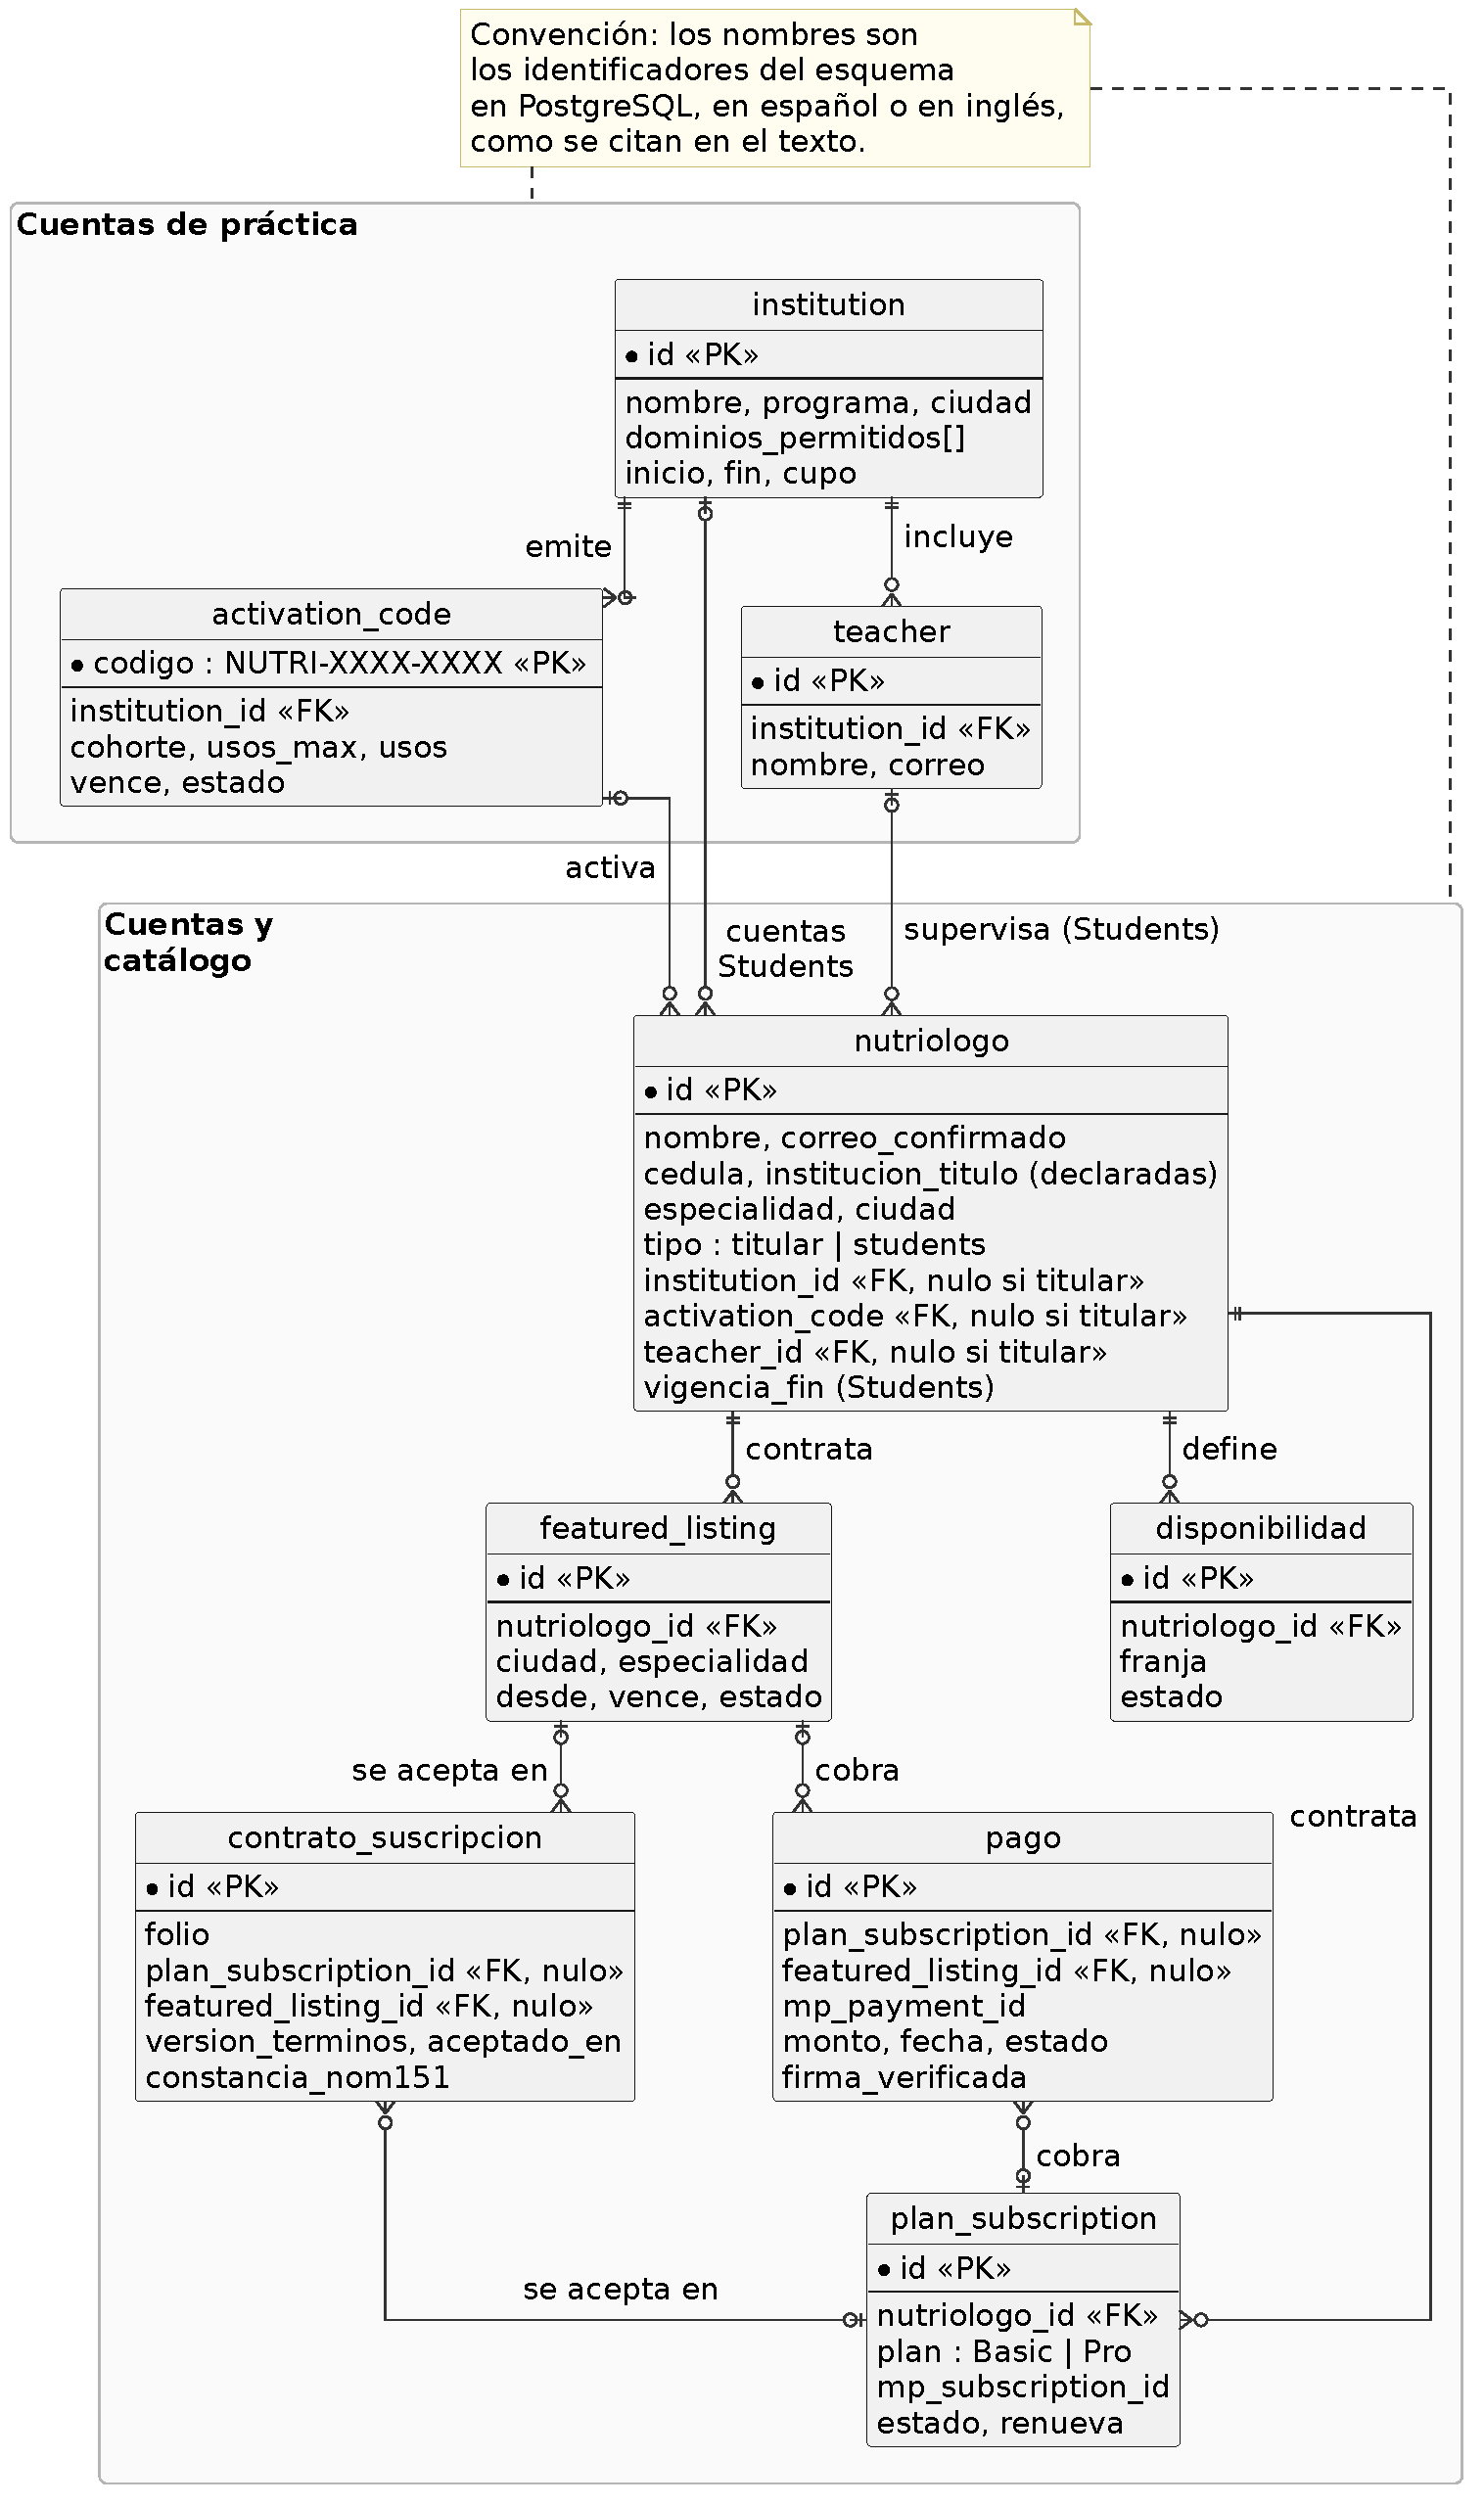
\includegraphics[width=\linewidth,height=0.84\textheight,keepaspectratio]{er-c.pdf}
    \caption{Cuentas de práctica, catálogo y suscripción.}
    \label{fig:er-c}
  \end{subfigure}
  \caption{Modelo entidad-relación de NutriApp (continuación).}
\end{figure}
 
\begin{figure}[H]
  \ContinuedFloat
  \captionsetup{list=no}
  \centering
  \begin{subfigure}{\linewidth}
    \centering
    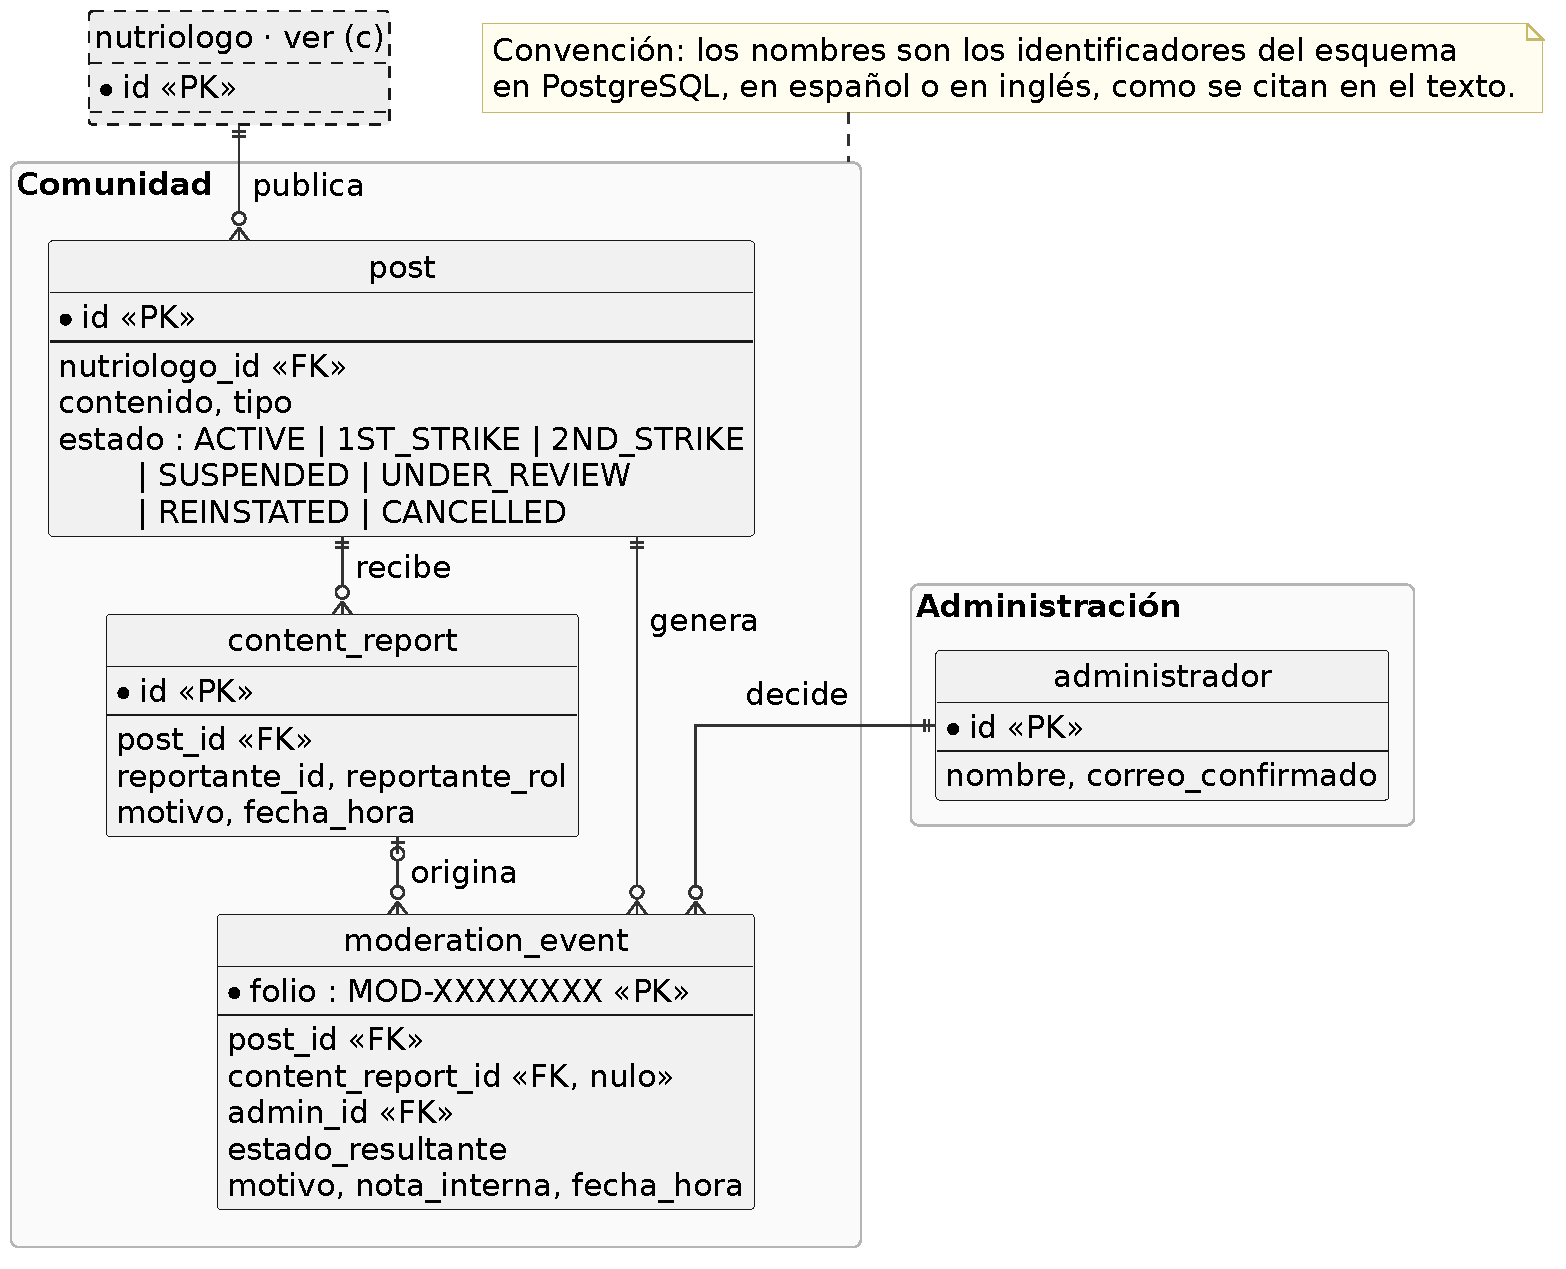
\includegraphics[width=\linewidth,height=0.84\textheight,keepaspectratio]{er-d.pdf}
    \caption{Comunidad y administración.}
    \label{fig:er-d}
  \end{subfigure}
  \caption{Modelo entidad-relación de NutriApp (continuación).}
\end{figure}
 
En el bloque clínico, cada \texttt{paciente} tiene un
\texttt{expediente} por cada nutriólogo que lo atiende, y ese
nutriólogo es el responsable de sus datos. El expediente guarda los
datos clínicos cifrados
con su propia llave de datos (sección~2.5.3) y un estado
(\textit{pendiente}, \textit{activo}, \textit{revocado} o \textit{bloqueado}); el campo
\texttt{fecha\_ultimo\_acto} marca el inicio de los cinco años de
conservación de la NOM-004, y \texttt{bloqueado\_desde} registra el
inicio del bloqueo cuando una cancelación procede (sección~2.5.5). En
el bloque de derechos y trazabilidad, \texttt{consentimiento} y
\texttt{arco\_request} se identifican por folio (\texttt{DEC-} y
\texttt{ARCO-}). El consentimiento registra el mecanismo con que se
otorgó, la versión del aviso aceptado, si el titular aceptó los avisos
por mensajería y, en su caso, la revocación. La solicitud ARCO registra
el nutriólogo que la resuelve, el tipo, el estado, las fechas de
presentación, resolución y ejecución
y, si procede la cancelación, \texttt{bloqueo\_hasta}, el fin del
bloqueo que el responsable fija conforme al plazo de prescripción
(RLFPDPPP, 2011, art.~107, fracc.~I); \texttt{bloqueado\_desde} y
\texttt{bloqueo\_hasta} son, por tanto, el inicio y el fin de ese
periodo. La entidad \texttt{incidente} registra la vulneración
detectada, su descripción y alcance, los expedientes afectados y la
fecha en que la plataforma alertó al nutriólogo responsable
(\texttt{alerta\_responsable\_en}); la fecha del aviso a los titulares
(\texttt{aviso\_titulares\_en}) la asienta el responsable, porque la
decisión de avisar y el envío son suyos (sección~2.4.2,
Tabla~\ref{tab:trazabilidad-2}).
\texttt{declaration\_log} conserva la copia inmutable de cada
declaración, y \texttt{audit\_log} registra quién consultó, modificó o
descargó cada expediente, junto con los intentos fallidos, el bloqueo,
la supresión, la destrucción de la llave y las notificaciones; su
referencia al expediente se anula tras la supresión, sin borrar el
registro. Las dos tablas forman la capa de aplicación del registro de
auditoría y se exportan juntas al depósito de registros de auditoría
(sección~5.2.1). Los mecanismos de la sección~5.1 añaden al modelo
tres entidades y varios campos: \texttt{aviso\_privacidad} (las
versiones del aviso de cada nutriólogo, a las que apunta
\texttt{consentimiento.aviso\_version}), \texttt{notificacion} (los
avisos dentro de la aplicación) y \texttt{constancia\_lote} (las
constancias diarias de la NOM-151); \texttt{paciente} guarda el número
móvil confirmado y la fecha de su invitación; \texttt{expediente}, la
llave de datos cifrada (\texttt{llave\_datos\_cifrada}); \texttt{adjunto},
el tipo, el tamaño y el resumen SHA-256; \texttt{arco\_request}, el
texto de la respuesta, el fundamento y las fechas límite calculadas;
\texttt{incidente}, el folio \texttt{INC-}, el estado y el administrador
que lo registra; \texttt{plan\_subscription}, el estado de la
suscripción (activa, en gracia, suspendida o terminada);
\texttt{nutriologo}, el estado de moderación de la sección~6.2.6; y
\texttt{induccion\_paso}, el avance de inducción de las cuentas
Students.
 
Las cuentas de práctica no crean un tipo de usuario aparte: un
estudiante es un \texttt{nutriologo} de tipo \textit{students},
ligado a la \texttt{institution} y al \texttt{activation\_code} con
que se activó, y sus pacientes llevan la marca \texttt{ficticio}.
La cédula y la institución que expidió el título se guardan como datos
declarados por el profesional, sin documento probatorio. El modelo
tampoco guarda datos de tarjeta: \texttt{plan\_subscription} conserva
el identificador de suscripción que devuelve Mercado Pago;
\texttt{pago} registra el identificador de cada cobro, el monto, la
fecha, el estado y el resultado de verificar la firma de la
notificación (sección~5.1); \texttt{contrato\_suscripcion} guarda el
folio, la versión de los términos aceptados, la fecha y la constancia
NOM-151 del contrato. \texttt{featured\_listing} no tiene relación
alguna con pacientes, porque ningún dato de pacientes interviene en el
orden del catálogo.
 
El recorrido de un dato de salud, del consentimiento del paciente a su
supresión, reparte las acciones entre el paciente, NutriApp y el
nutriólogo (Figura~\ref{fig:flujo-datos}): al vencer la conservación
mínima o el periodo de bloqueo, NutriApp avisa al nutriólogo, y el
borrado criptográfico ocurre solo si él confirma la supresión; si no la
confirma, el expediente se conserva. Los estados que el expediente
recorre en ese trayecto se detallan en la Figura~\ref{fig:uml-estados}.
 
\begin{landscape}
\begin{figure}[H]
  \centering
  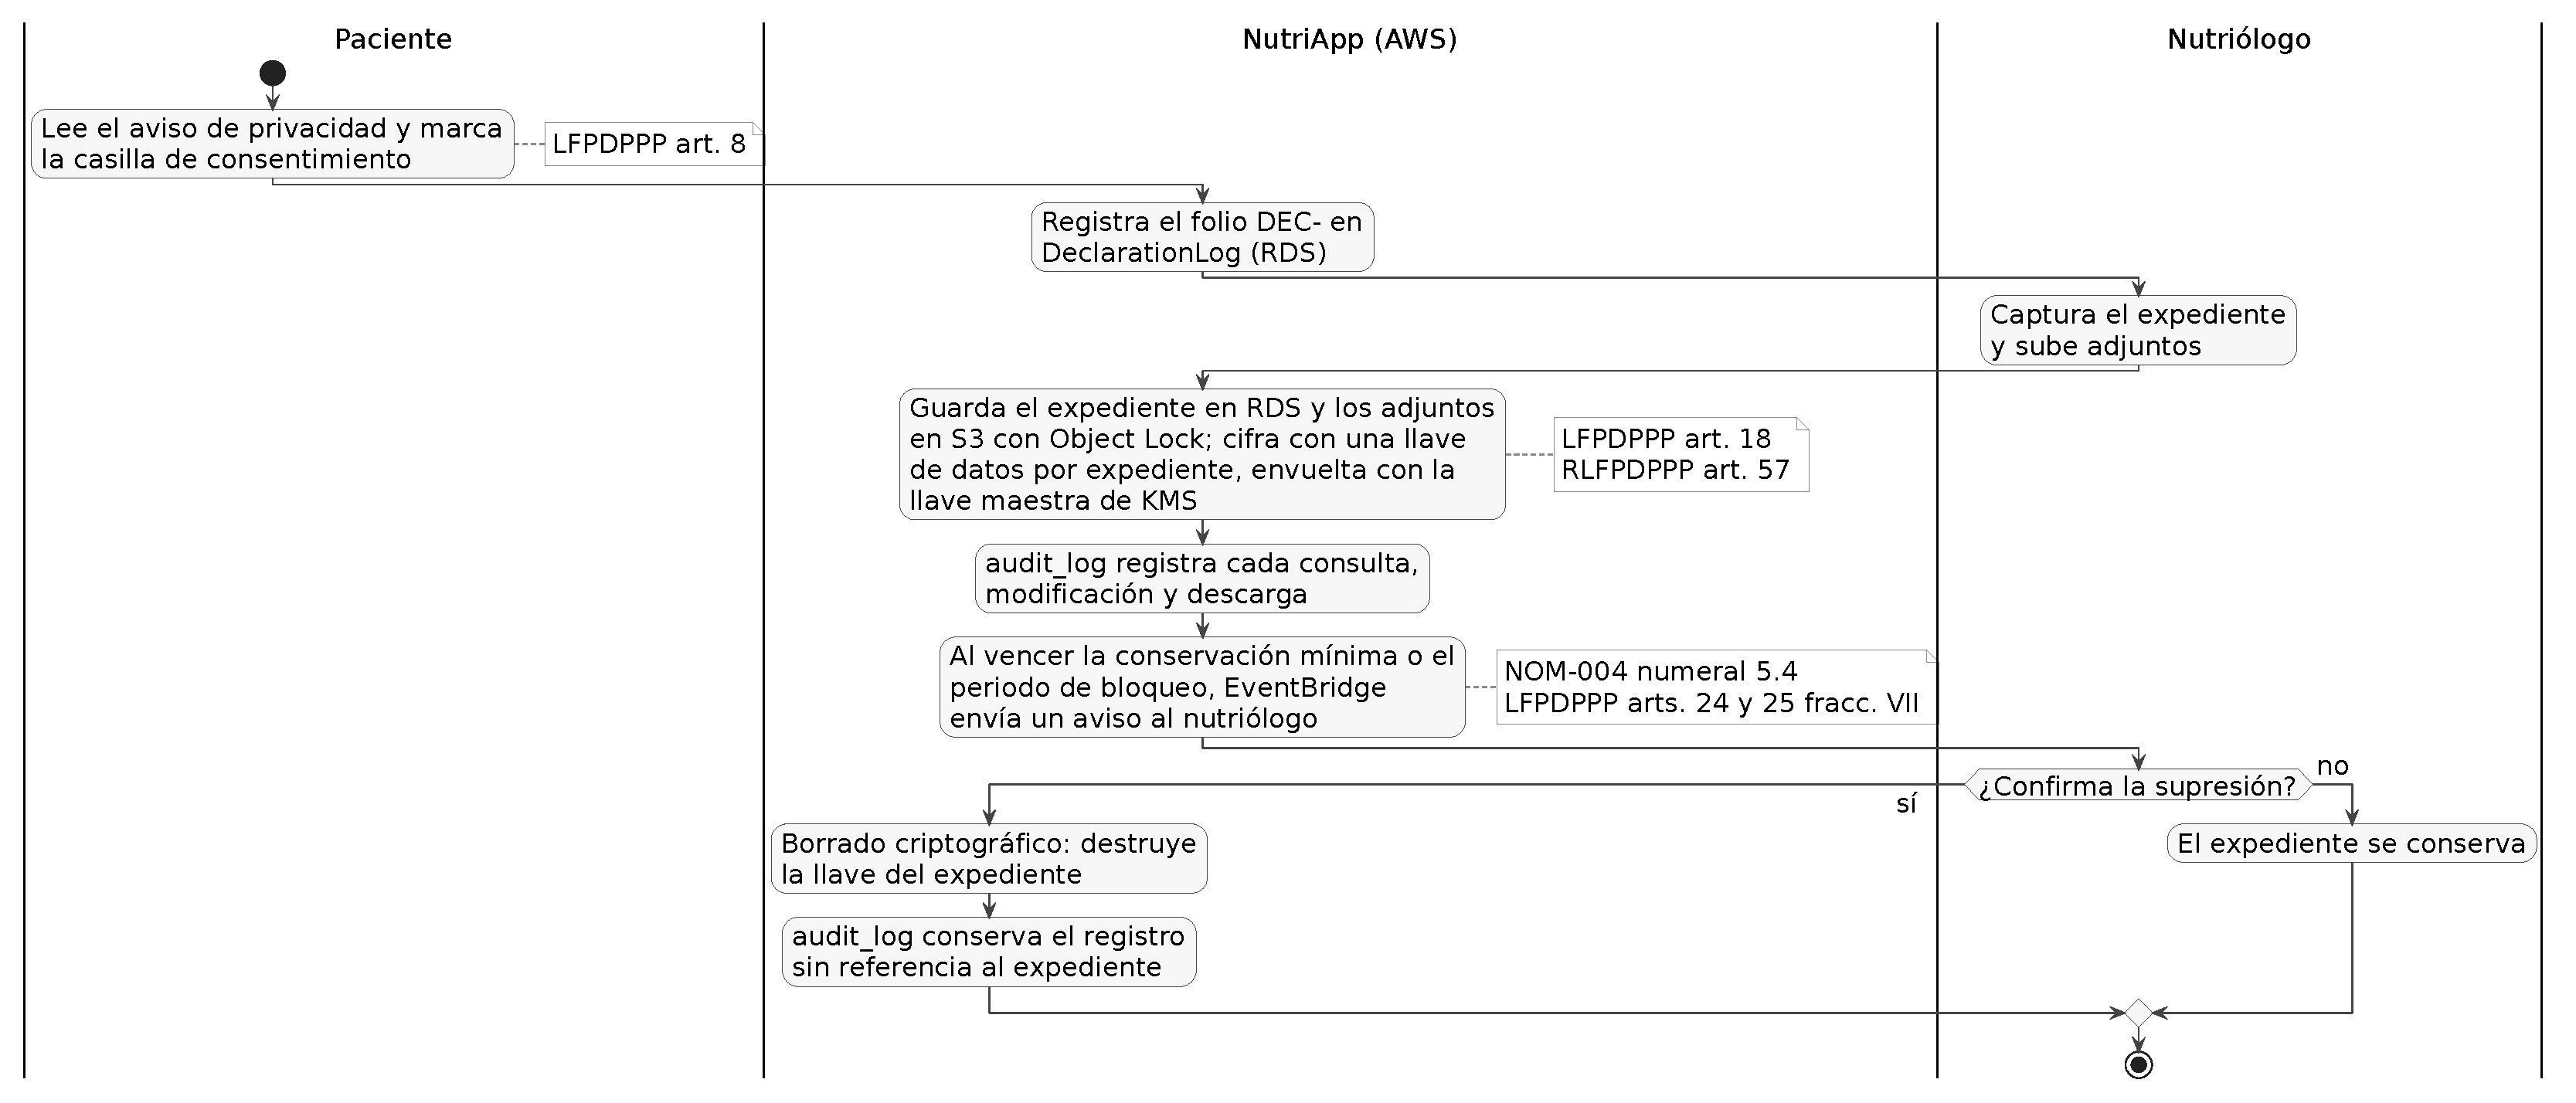
\includegraphics[width=\linewidth,height=0.84\textheight,keepaspectratio]{flujo-datos.pdf}
  \caption{Recorrido del dato de salud en NutriApp, del consentimiento a la supresión confirmada por el nutriólogo.}
  \label{fig:flujo-datos}
\end{figure}
\end{landscape}

\subsubsection{Diagrama de estados del expediente}
 
La Figura~\ref{fig:uml-estados} sigue al expediente a lo largo de su
vida con los valores del campo \texttt{estado} y el estado final de
supresión. El alta en \texttt{AddPatient} lo crea \textit{pendiente de
consentimiento}: no admite datos de salud hasta que el paciente marca
la casilla obligatoria y el sistema registra el folio \texttt{DEC-}
(LFPDPPP, 2025, art.~8). Con el consentimiento pasa a \textit{activo}. Si el paciente revoca el consentimiento, pasa a \textit{revocado}, en el que deja de admitir datos nuevos y lo registrado sigue bajo la conservación de la NOM-004, sin efectos retroactivos (LFPDPPP, 2025, art.~7).
Una solicitud de cancelación tiene dos salidas. Si el nutriólogo la
niega porque corre la conservación mínima, el expediente sigue activo
(LFPDPPP, 2025, art.~25, fracc.~VII; NOM-004-SSA3-2012, 2012,
numeral~5.4). Si procede, la resuelve y la ejecuta en los plazos del
artículo~31, y el expediente pasa a \textit{bloqueado} hasta el plazo
de prescripción (LFPDPPP, 2025, art.~24; RLFPDPPP, 2011, art.~107,
fracc.~I). A \textit{suprimido} se llega por dos caminos: al vencer la
conservación mínima de un expediente activo o revocado, o al vencer el periodo de
bloqueo. En los dos, un aviso programado llega al nutriólogo y el
borrado criptográfico solo se ejecuta con su confirmación
(sección~2.5.5).
 
\begin{figure}[H]
  \centering
  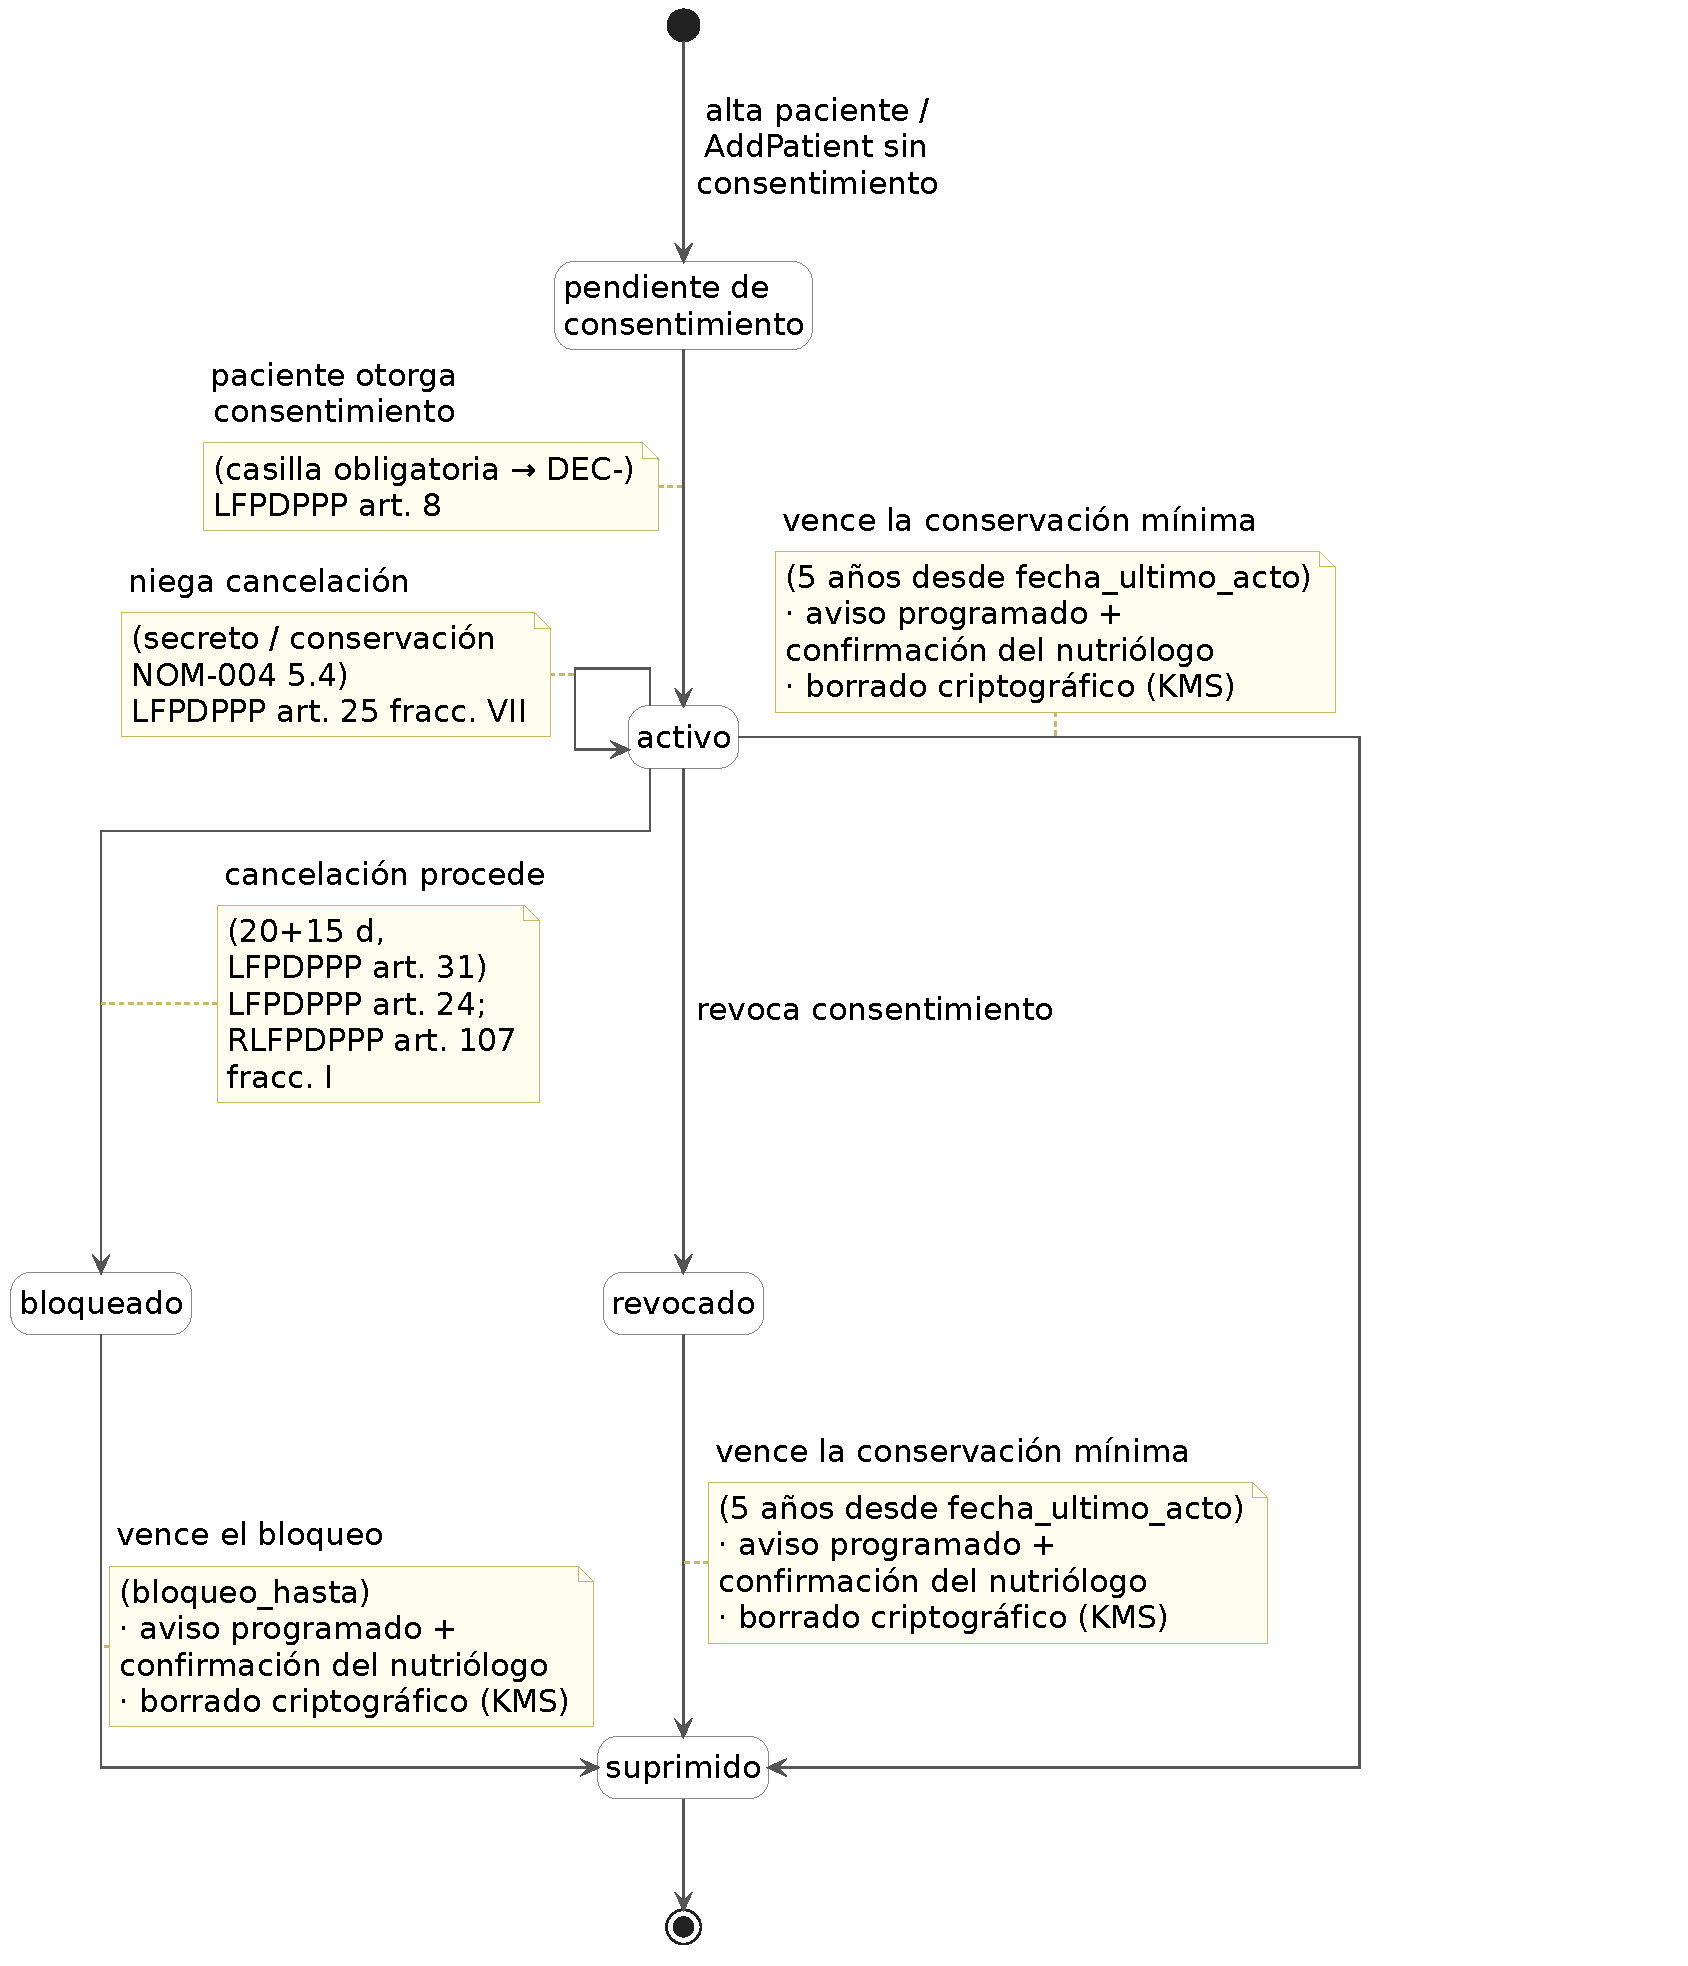
\includegraphics[width=\linewidth,height=0.80\textheight,keepaspectratio]{uml-estados-expediente.pdf}
  \caption{Diagrama de estados del expediente clínico.}
  \label{fig:uml-estados}
\end{figure}

% ═══════════════════════════════════════════════════════════════════════════
\section{Demostración del diseño: maquetas y prueba piloto}
% ═══════════════════════════════════════════════════════════════════════════
 
Este capítulo muestra el diseño del capítulo~5 convertido en algo
que se puede recorrer: un producto mínimo viable (MVP), formado por
los módulos que atienden las obligaciones de las
Tablas~\ref{tab:trazabilidad-1} y~\ref{tab:trazabilidad-2} y por los
de uso diario que justifica la sección~6.4. El MVP
se representa en maquetas navegables construidas en Figma Make con
React, TypeScript y Tailwind. Siguiendo el criterio de Peffers et al.
(2007) adoptado en la sección~4.1.2, la maqueta es la forma evaluable
del artefacto; ninguna pantalla ha operado con datos de personas
reales. Sobre ella, un revisor con conocimiento del marco normativo
puede comprobar pantalla por pantalla si el flujo muestra lo que la
ley exige, y el grupo focal de nutriólogos con práctica clínica la revisa
como caso en la
prueba piloto. El capítulo presenta, en este orden, los
requerimientos, las maquetas por flujo, la prueba piloto y la
justificación del alcance.
 
% ─────────────────────────────────────────────────────────────────────────
\subsection{Requerimientos mínimos del sistema}
% ─────────────────────────────────────────────────────────────────────────
 
Los requerimientos del MVP se organizan en tres grupos.
 
\textbf{Seguridad técnica} (Ley Federal de Protección de Datos Personales en Posesión de los Particulares [LFPDPPP], 2025, art.~18; NOM-024-SSA3-2012,
2012, numerales~6.6.1, 6.6.3 y~6.6.4; sección~2.5): los datos se cifran con
AES-256 (Advanced Encryption Standard) en reposo y con TLS~1.3 (Transport Layer Security) en tránsito. La autenticación
multifactor, con código TOTP de una aplicación de autenticación, es
obligatoria para el nutriólogo, el docente y el administrador, y el
registro de auditoría abarca las tres capas descritas en el marco
técnico. La
eliminación procede por bloqueo y supresión: al vencer la retención o
el bloqueo, el sistema avisa al nutriólogo y, con su confirmación,
destruye la llave de datos del expediente (sección~2.5.5).
 
\textbf{Derechos del titular} (LFPDPPP, 2025, arts.~8, 15 y~22--34): el
consentimiento lo otorga el propio paciente, con acción afirmativa y
sin casillas premarcadas, y se registra con folio y fecha. El aviso de
privacidad, que el nutriólogo edita y publica por versiones desde su
perfil (sección~5.1), es accesible desde cualquier pantalla. El módulo de derechos de acceso, rectificación, cancelación y oposición (ARCO)
recibe la solicitud, registra la resolución del nutriólogo y notifica
al titular, con respuesta en veinte días y ejecución en los quince
siguientes (art.~31).
 
\textbf{Trazabilidad normativa} (Reglamento de la Ley Federal de Protección de Datos Personales en Posesión de los Particulares [RLFPDPPP], 2011, arts.~48, fracc.~X,
y~61): el inventario de datos se clasifica por sensibilidad.
NutriApp entrega al nutriólogo el inventario de los datos que trata la
plataforma como insumo de su propio inventario, que abarca también los
soportes ajenos a ella (RLFPDPPP, 2011, art.~61, fracc.~I); esa entrega
no tiene maqueta en la prueba piloto. Las
declaraciones profesionales se registran en el \texttt{DeclarationLog}
con folio único y copia de los datos declarados en cada firma. El
titular recibe con folio la resolución de su solicitud, con el periodo
de bloqueo y la fecha prevista de supresión; la supresión final la
confirma el nutriólogo y queda en el registro de auditoría. Ante una
vulneración, la plataforma registra el incidente con folio, a partir
de las alarmas definidas en la sección~5.1, y alerta al nutriólogo, que decide y envía el aviso al titular (LFPDPPP,
2025, art.~19; Tabla~\ref{tab:trazabilidad-2}); ese registro es
interno y no tiene maqueta en la prueba piloto.
 
Tres obligaciones sanitarias quedan fuera del MVP y se declaran aquí
para delimitar el alcance. La NOM-004-SSA3-2012 fija los datos generales de todo
expediente (numeral~5.2), los requisitos comunes de las notas, que
llevan identificación del paciente y fecha, hora, nombre y firma de
quien las elabora (numerales~5.9 a~5.11), y los apartados de la
historia clínica (numeral~6.1). La NOM-024 exige que el sistema
permita el uso de la firma electrónica avanzada del profesional para
la información que el prestador determine en su gestión de seguridad
(numeral~6.6.2), y que permita exportar la información del paciente
conforme a la normativa de protección de datos (numeral~6.6.6). El
expediente de NutriApp guarda notas de nutrición como texto libre con
autor, fecha y hora, lo que corresponde a esa parte del numeral~5.10,
pero no incorpora la estructura de la historia clínica, ni ofrece la
firma electrónica avanzada, ni la exportación estructurada. Las tres
se documentan como siguiente paso en la sección~8.3.
 
El criterio de completitud que aplica la sección~6.4 se refiere, por
tanto, a las obligaciones de las Tablas~\ref{tab:trazabilidad-1}
y~\ref{tab:trazabilidad-2} y no a la totalidad de las normas
sanitarias. También quedan fuera los módulos de inteligencia
artificial para análisis nutricional, la integración con laboratorios,
la telemedicina y la segunda versión del módulo social, porque
requieren análisis normativos en materia sanitaria y de
responsabilidad profesional que exceden este caso.
 
% ─────────────────────────────────────────────────────────────────────────
\subsection{Maquetas por flujo}
% ─────────────────────────────────────────────────────────────────────────
 
Las maquetas se presentan por flujo, porque una obligación legal rara
vez cabe en una sola pantalla. En cada flujo se indica qué obligación
demuestra y qué evidencia debe verse en la maqueta. Los tres primeros
corresponden, en ese orden, a los casos CP-01, CP-02 y CP-03 de la
Tabla~\ref{tab:casos-prueba}, que verifican esa evidencia. El
Anexo~\ref{anexo:capturas} reunirá las capturas de las pantallas principales del prototipo de interfaz y el
repositorio del proyecto contiene las maquetas navegables y el código
(NutriApp, 2026).
 
\subsubsection{Registro del nutriólogo y consentimiento del paciente}
 
El nutriólogo se registra en la pantalla de alta profesional
(\texttt{NutritionistRegister}) con su cédula profesional y la
institución que expidió su título. Ahí firma una declaración bajo
protesta, que el \texttt{DeclarationLog} conserva, e inscribe el
segundo factor en la pantalla \texttt{MFASetup}, que muestra el código
QR para la aplicación de autenticación y comprueba un primer código
TOTP, antes de poder entrar a cualquier expediente (sección~5.1). La veracidad de la cédula y del título es responsabilidad
del nutriólogo, que la asume en esa declaración; NutriApp no los
verifica. Exhibir la institución que expidió el título y el número de
cédula, también en la publicidad, es obligación de quien ejerce la
profesión (Ley General de Salud [LGS], 1984/2026, art.~83). NutriApp solo habilita esos
campos y muestra un recordatorio. Antes de publicar su ficha, una
ventana emergente le indica al nutriólogo que los datos capturados
deben coincidir con su registro en la consulta pública de cédulas
profesionales de la Secretaría de Educación Pública (s.f.), y que la
ficha los mostrará tal como los declaró. La misma ventana le recuerda
que la responsabilidad por su veracidad es suya. La ficha se publica
solo cuando el nutriólogo confirma esa ventana; el
\texttt{DeclarationLog} registra la fecha y hora de la confirmación.
 
El flujo de consentimiento cambió respecto del diseño inicial, en el
que era el nutriólogo quien marcaba la casilla al crear el
expediente. La LFPDPPP exige para datos sensibles el consentimiento
expreso y por escrito del titular, con firma autógrafa, electrónica o
mecanismo de autenticación (LFPDPPP, 2025, art.~8), y lo define como
manifestación de la voluntad libre, específica e informada (art.~2,
fracc.~IV). En la maqueta, por tanto, es el paciente quien consiente:
en su propia sesión autenticada desde su dispositivo o, en el
consultorio, sobre el dispositivo del nutriólogo, autenticándose él
mismo. La cuenta del paciente la crea la plataforma cuando el
nutriólogo lo da de alta: \texttt{AddPatient} captura solo nombre y
correo, una Lambda crea el usuario en Cognito como administrador y
Cognito envía por SES la invitación con contraseña temporal, que caduca
a los siete días y puede reenviarse desde \texttt{PatientList} (AWS,
s.f.-h). Al primer acceso el paciente confirma su correo, fija su
contraseña y encuentra como primera pantalla la de consentimiento; si
el correo ya tiene cuenta porque otro nutriólogo lo atiende, no se crea
otra: el expediente nuevo queda pendiente en su panel hasta que
consiente. En el consultorio, el consentimiento abre una sesión
aislada del paciente en el dispositivo del nutriólogo, que se cierra al
confirmar o a los cinco minutos.
 
La pantalla de consentimiento muestra el aviso de privacidad
completo, con opción de descarga en PDF, y dos casillas sin marcar: la
obligatoria para el tratamiento de datos de salud y una opcional para
recibir avisos también por WhatsApp o mensaje de texto (SMS), que al
marcarse pide el número móvil y lo confirma con un código de un solo
uso (sección~5.1). Los avisos con efecto
jurídico llegan siempre al correo confirmado de la cuenta y ningún
mensaje lleva contenido clínico (sección~2.5.5). Al confirmar, el
sistema genera el folio \texttt{DEC-XXXXXXXX} y el
\texttt{DeclarationLog} guarda la identidad del titular, el mecanismo
de autenticación usado, la versión del aviso, la fecha y la hora, y
una copia de lo consentido. Hasta ese momento el expediente permanece
en estado «pendiente de consentimiento» y no admite el registro de
ningún dato de salud. El nutriólogo ve ese estado en su lista de
pacientes (\texttt{PatientList}) y recibe un aviso emergente cuando el
paciente completa el trámite (Figura~\ref{fig:maq-consentimiento}).
 
\begin{landscape}
\begin{figure}[H]
  \centering
  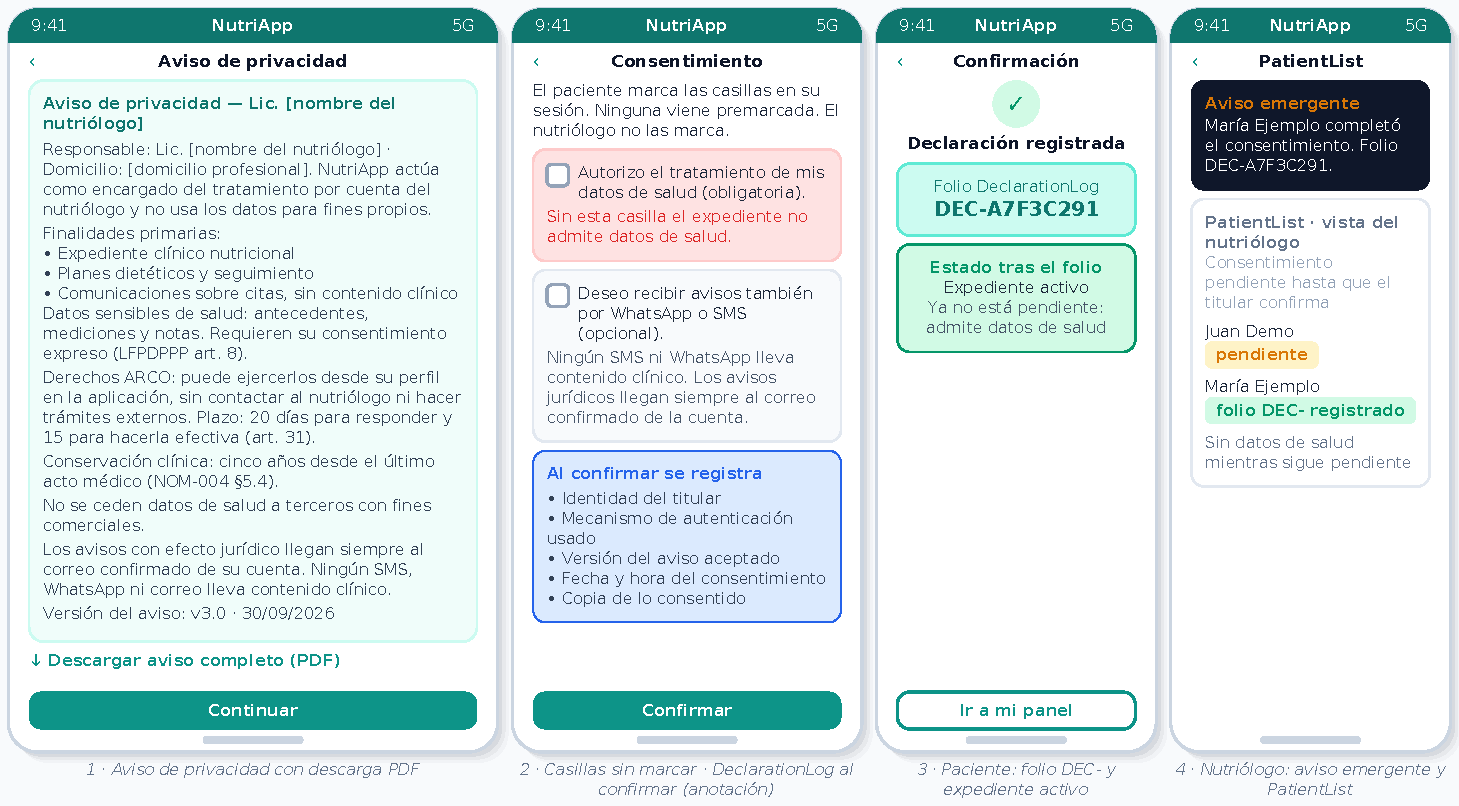
\includegraphics[width=\linewidth,height=0.88\textheight,keepaspectratio]{maqueta-consentimiento.pdf}
  \caption{Maqueta del flujo de consentimiento del paciente: aviso de
  privacidad, casillas sin marcar, folio y estado del expediente.}
  \label{fig:maq-consentimiento}
\end{figure}
\end{landscape}
 
\subsubsection{Alta de paciente y expediente}
 
Una vez registrado el consentimiento, las pantallas de alta de paciente
(\texttt{AddPatient}) y de expediente (\texttt{PatientDetail}) admiten
datos de identificación, antecedentes, mediciones, notas de nutrición con
autor, fecha y hora, y adjuntos en PDF, JPEG o PNG de hasta 5~MB por
archivo (sección~5.1). Sin ese consentimiento el alta no se
completa y el expediente sigue en el estado pendiente del flujo
anterior; el caso CP-02 parte, por eso, de un consentimiento ya
registrado. Cada pantalla recibe solo los campos que esa vista
necesita, conforme a la regla de proporcionalidad definida en la
sección~5.1. Toda consulta, modificación, descarga e intento fallido
de acceso queda en el registro de auditoría, y el paciente puede
consultar en su panel (\texttt{Dashboard}) una vista derivada de ese
registro: quién accedió a su expediente y cuándo. El plan de
alimentación se asigna desde la pantalla \texttt{AssignDiet} a partir
de la biblioteca de plantillas (\texttt{TemplateLibrary}); el paciente
lo consulta en su dieta actual (\texttt{CurrentDiet}) y en el
seguimiento de avances (\texttt{ProgressTracking}). Estas pantallas
forman el recorrido del expediente (Figura~\ref{fig:maq-expediente}).
 
\begin{landscape}
\begin{figure}[H]
  \centering
  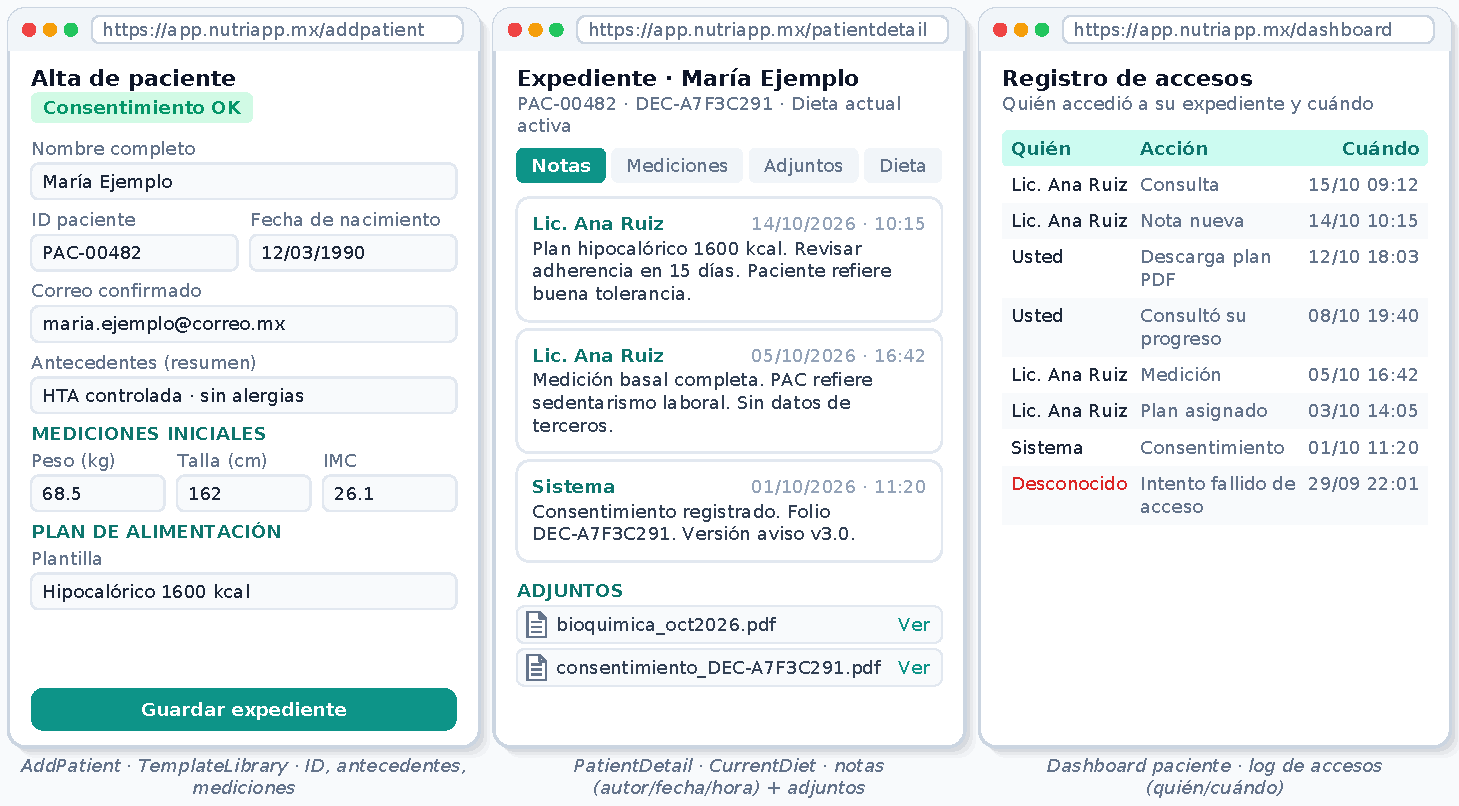
\includegraphics[width=\linewidth,height=0.88\textheight,keepaspectratio]{maqueta-expediente.pdf}
  \caption{Maqueta del alta de paciente y del expediente con registro
  de accesos.}
  \label{fig:maq-expediente}
\end{figure}
\end{landscape}
 
\subsubsection{Derechos ARCO y cancelación}
 
El paciente ejerce sus derechos desde su perfil, sin contactar al
nutriólogo ni iniciar trámites externos: cuatro tarjetas presentan
acceso, rectificación, cancelación y oposición en lenguaje llano y
generan una solicitud con folio. La cancelación es el caso que la
maqueta debe explicar con más cuidado, porque no es inmediata ni
irrevocable, como decía el diseño inicial. El diálogo de confirmación
lo explica por partes. La solicitud la resuelve el nutriólogo como
responsable en un plazo de veinte días y, si procede, la ejecuta en
los quince siguientes (LFPDPPP, 2025, art.~31).
Mientras corre la conservación mínima de cinco años contados desde el
último acto médico, el responsable no está obligado a cancelar el
expediente clínico (LFPDPPP, 2025, art.~25, fracc.~VII;
NOM-004-SSA3-2012, 2012, numeral~5.4), y el diálogo se lo explica al
paciente. Si la cancelación procede, el expediente pasa a estado de
bloqueo (LFPDPPP, 2025, art.~24) y se conserva cifrado, fuera de la
operación diaria, hasta el plazo de prescripción que fija el
responsable (RLFPDPPP, 2011, art.~107, fracc.~I). La respuesta, con
folio, el periodo de bloqueo y la fecha prevista de supresión, llega al
correo confirmado del titular. Una vez enviada, se suprimen los datos de la
cuenta y de contacto y las preferencias de notificación, salvo que el
titular tenga otro expediente activo en la plataforma; en ese caso solo
se desvincula al nutriólogo que resolvió. Un registro posterior del
titular genera una cuenta nueva. El aviso al nutriólogo al vencer la conservación o el
bloqueo y el borrado criptográfico con su confirmación siguen la
secuencia de la sección~2.5.5.
 
El nutriólogo resuelve desde \texttt{PatientDetail} con un texto de
respuesta y, cuando niega, el fundamento, que \texttt{arco\_request}
conserva; en una solicitud de acceso, la plataforma genera y adjunta
una copia simple del expediente en PDF (identificación, antecedentes,
notas, mediciones, plan vigente y lista de adjuntos), sin la estructura
de exportación del numeral~6.6.6 de la NOM-024, que sigue fuera del
MVP; la rectificación se ejecuta como modificación del expediente
ligada al folio en el \texttt{audit\_log}, y la oposición se resuelve
con texto y, si procede, con bloqueo. La revocación del consentimiento
tiene su propio botón junto a las cuatro tarjetas, con un diálogo que
explica que no tiene efectos retroactivos (LFPDPPP, 2025, art.~7) y
que el expediente sigue sujeto a la conservación de la NOM-004, y
genera el registro equivalente al consentimiento
(Figura~\ref{fig:uml-cu-a}).
 
Al nutriólogo, el expediente (\texttt{PatientDetail}) le muestra las
solicitudes activas con folio, tipo, fecha, días restantes y estado;
la función diaria de la sección~5.1 genera un aviso en la aplicación y
en el correo cuando quedan cinco días o menos del plazo del
artículo~31, y la alarma de CloudWatch sobre la misma métrica alerta a
la operación de NutriApp (Figura~\ref{fig:maq-arco}).
 
\begin{landscape}
\begin{figure}[H]
  \centering
  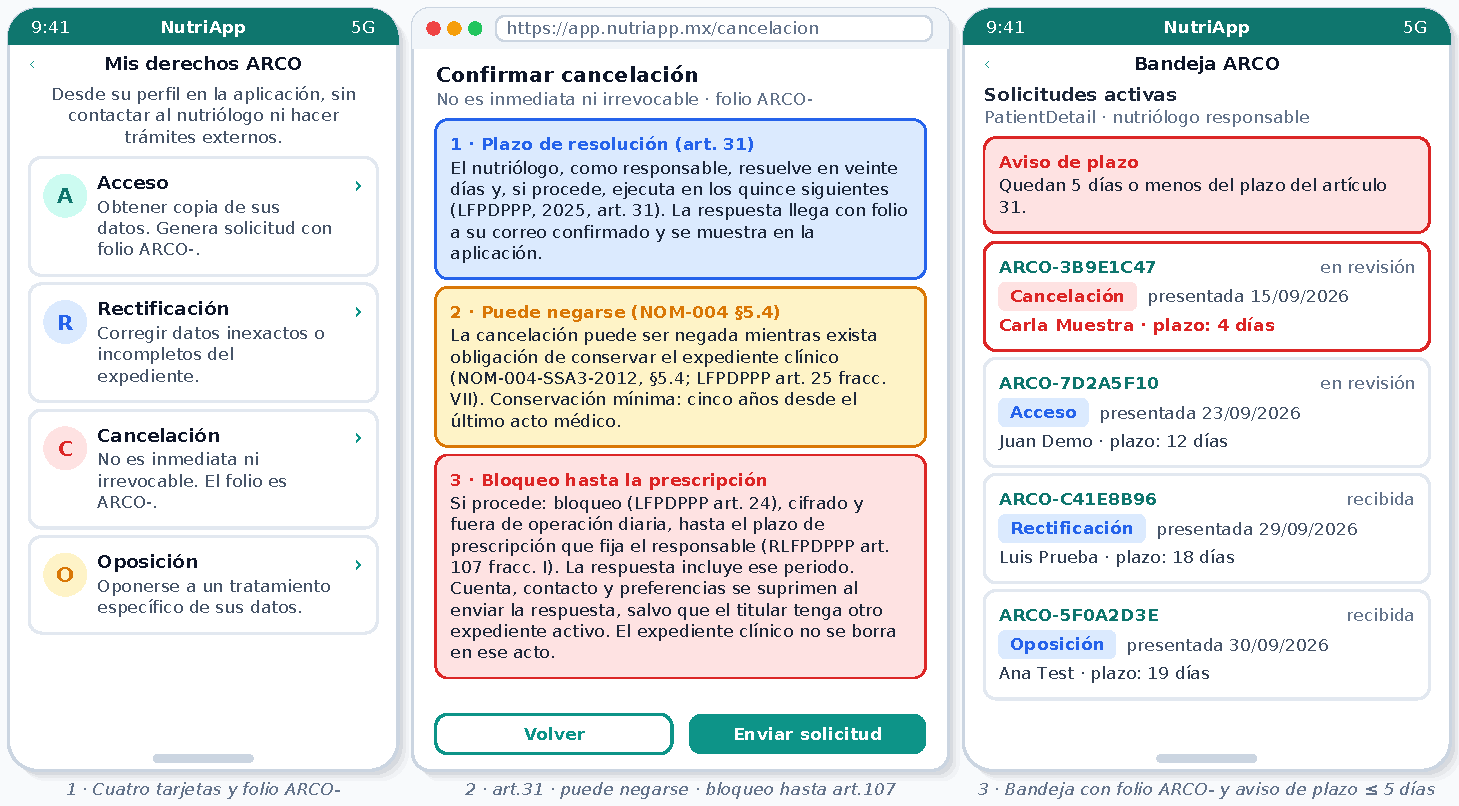
\includegraphics[width=\linewidth,height=0.88\textheight,keepaspectratio]{maqueta-arco.pdf}
  \caption{Maqueta del módulo ARCO: solicitud del paciente, diálogo de
   cancelación con bloqueo y plazo, y bandeja del nutriólogo.}
  \label{fig:maq-arco}
\end{figure}
\end{landscape}
 
\subsubsection{Catálogo y reserva de cita}
 
\begin{sloppypar}
El paciente busca nutriólogo por ciudad y especialidad en el buscador
(\texttt{FindNutritionist}). Los resultados se ordenan por
disponibilidad, cercanía declarada y especialidad; ningún dato de
pacientes interviene en el orden. Entre los cinco primeros
resultados, a lo sumo dos llevan la etiqueta «Patrocinado», que
corresponde al servicio de exposición cuyas condiciones comerciales se
proponen como trabajo posterior (sección~8.3.1). La
tarjeta de cada profesional muestra la institución que expidió su
título y el número de cédula que declaró, como exige la publicidad de
servicios de salud (Reglamento de la Ley General de Salud en Materia
de Publicidad, 2000/2022, art.~19). La transparencia sustituye a la
verificación: junto a esos datos, la ficha indica que los declaró el
profesional bajo su responsabilidad y enlaza a la consulta pública de
cédulas de la Secretaría de Educación Pública (s.f.), para que el
paciente pueda comprobarlos por su cuenta. Un enlace junto al criterio
de orden explica cómo se ordenan los resultados.
\end{sloppypar}
 
La reserva sigue la secuencia de la Figura~\ref{fig:uml-seq}: el
paciente elige una franja horaria, inicia sesión y confirma en la
pantalla de confirmación (\texttt{ConfirmAppointment}). El nutriólogo
recibe la solicitud en su gestor de citas
(\texttt{AppointmentsManager}) con 48 horas para aceptarla; si no
responde, el sistema sugiere alternativas. Las citas se notifican
únicamente dentro de la aplicación (Figura~\ref{fig:maq-catalogo}).
 
\begin{landscape}
\begin{figure}[H]
  \centering
  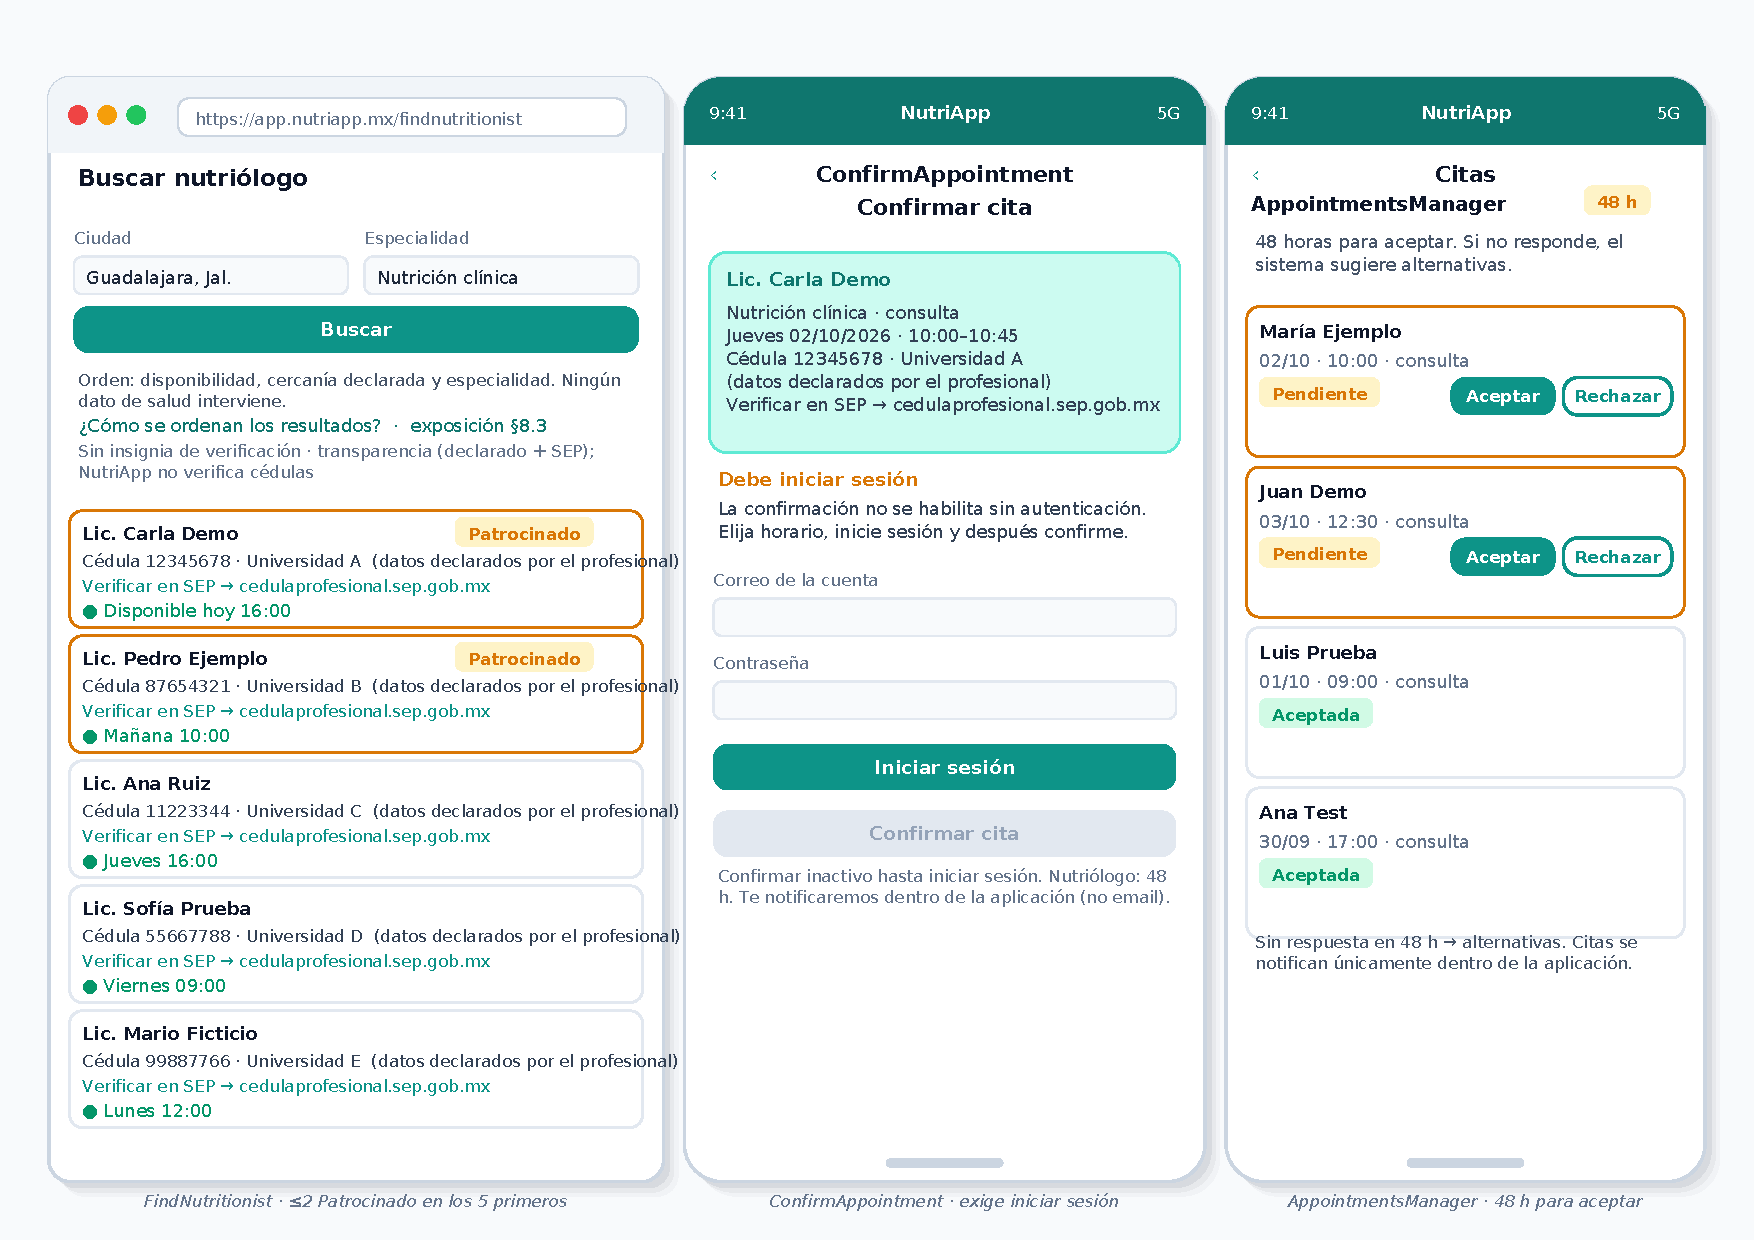
\includegraphics[width=\linewidth,height=0.88\textheight,keepaspectratio]{maqueta-catalogo.pdf}
  \caption{Maqueta del catálogo con resultados patrocinados
  etiquetados, cédula declarada por el profesional y reserva de cita.}
  \label{fig:maq-catalogo}
\end{figure}
\end{landscape}
 
\subsubsection{Cuentas de práctica: institución, códigos de activación y Students}
 
El MVP incluye cuentas de práctica para estudiantes de nutrición. Por
regla de diseño, ningún estudiante se registra por sí mismo. Primero
el administrador da de alta a la institución y al programa académico
en el panel de instituciones (\texttt{AdminInstitutions}), con la
lista de dominios de correo permitidos, la vigencia del semestre, el
cupo y las cuentas docentes. Después genera códigos de activación
(\texttt{ActivationCodes}) con usos máximos y fecha de vencimiento.
 
El estudiante activa su cuenta (\texttt{StudentsActivation}) en tres
pasos: introduce un código vigente, confirma un correo cuyo dominio
está en la lista de su institución, y acepta el aviso de privacidad y
los términos en casillas sin marcar. Una de esas casillas declara que
la cuenta solo funciona con pacientes ficticios. Al crearse la cuenta,
una función genera diez pacientes ficticios etiquetados como usuarios
de prueba, sin cuenta de Cognito ni correo, con expediente activo y un
consentimiento marcado como ficticio (folio \texttt{DEC-FIC-XXXXXXXX})
para que el resto de los flujos pueda practicarse; \texttt{AddPatient}
queda deshabilitado en estas cuentas, que exigen el mismo segundo
factor que el titular. Los expedientes de práctica se generan así con datos
ficticios y la cuenta declara que solo debe usarse con ellos; mientras
se use de ese modo, no contienen datos de ninguna persona identificada
o identificable (LFPDPPP, 2025, art.~2, fracc.~V) y no se les aplica
la conservación de la NOM-004. Si un estudiante captura datos reales,
el tratamiento queda sujeto a la LFPDPPP y los términos de uso lo
prohíben. Los datos del propio estudiante sí son datos personales, y
se tratan conforme al aviso de privacidad que acepta al activar la
cuenta. La cuenta vence con el semestre de la institución, con aviso
por correo y en la aplicación quince días antes; treinta días después
del vencimiento, la función programada suprime la cuenta y sus
expedientes ficticios, sin conservación de la NOM-004, y conserva los
datos del estudiante solo el tiempo que declara el aviso de privacidad
que aceptó. Al egresar, quien quiera seguir usando NutriApp se
registra como nutriólogo titular en un plan de pago. El docente
responsable, asignado por el código de activación con que el
estudiante se dio de alta, ve en su panel
(\texttt{TeacherDashboard}) los expedientes ficticios de sus
estudiantes en modo de solo lectura, el avance del módulo de inducción
(la secuencia guiada de los flujos del MVP sobre los pacientes
ficticios: alta de datos, nota y adjunto, plan, y solicitud y
resolución ARCO simuladas, con una fila por paso completado en
\texttt{induccion\_paso}) y el reporte semestral
(Figura~\ref{fig:maq-students}).
 
\begin{landscape}
\begin{figure}[H]
  \centering
  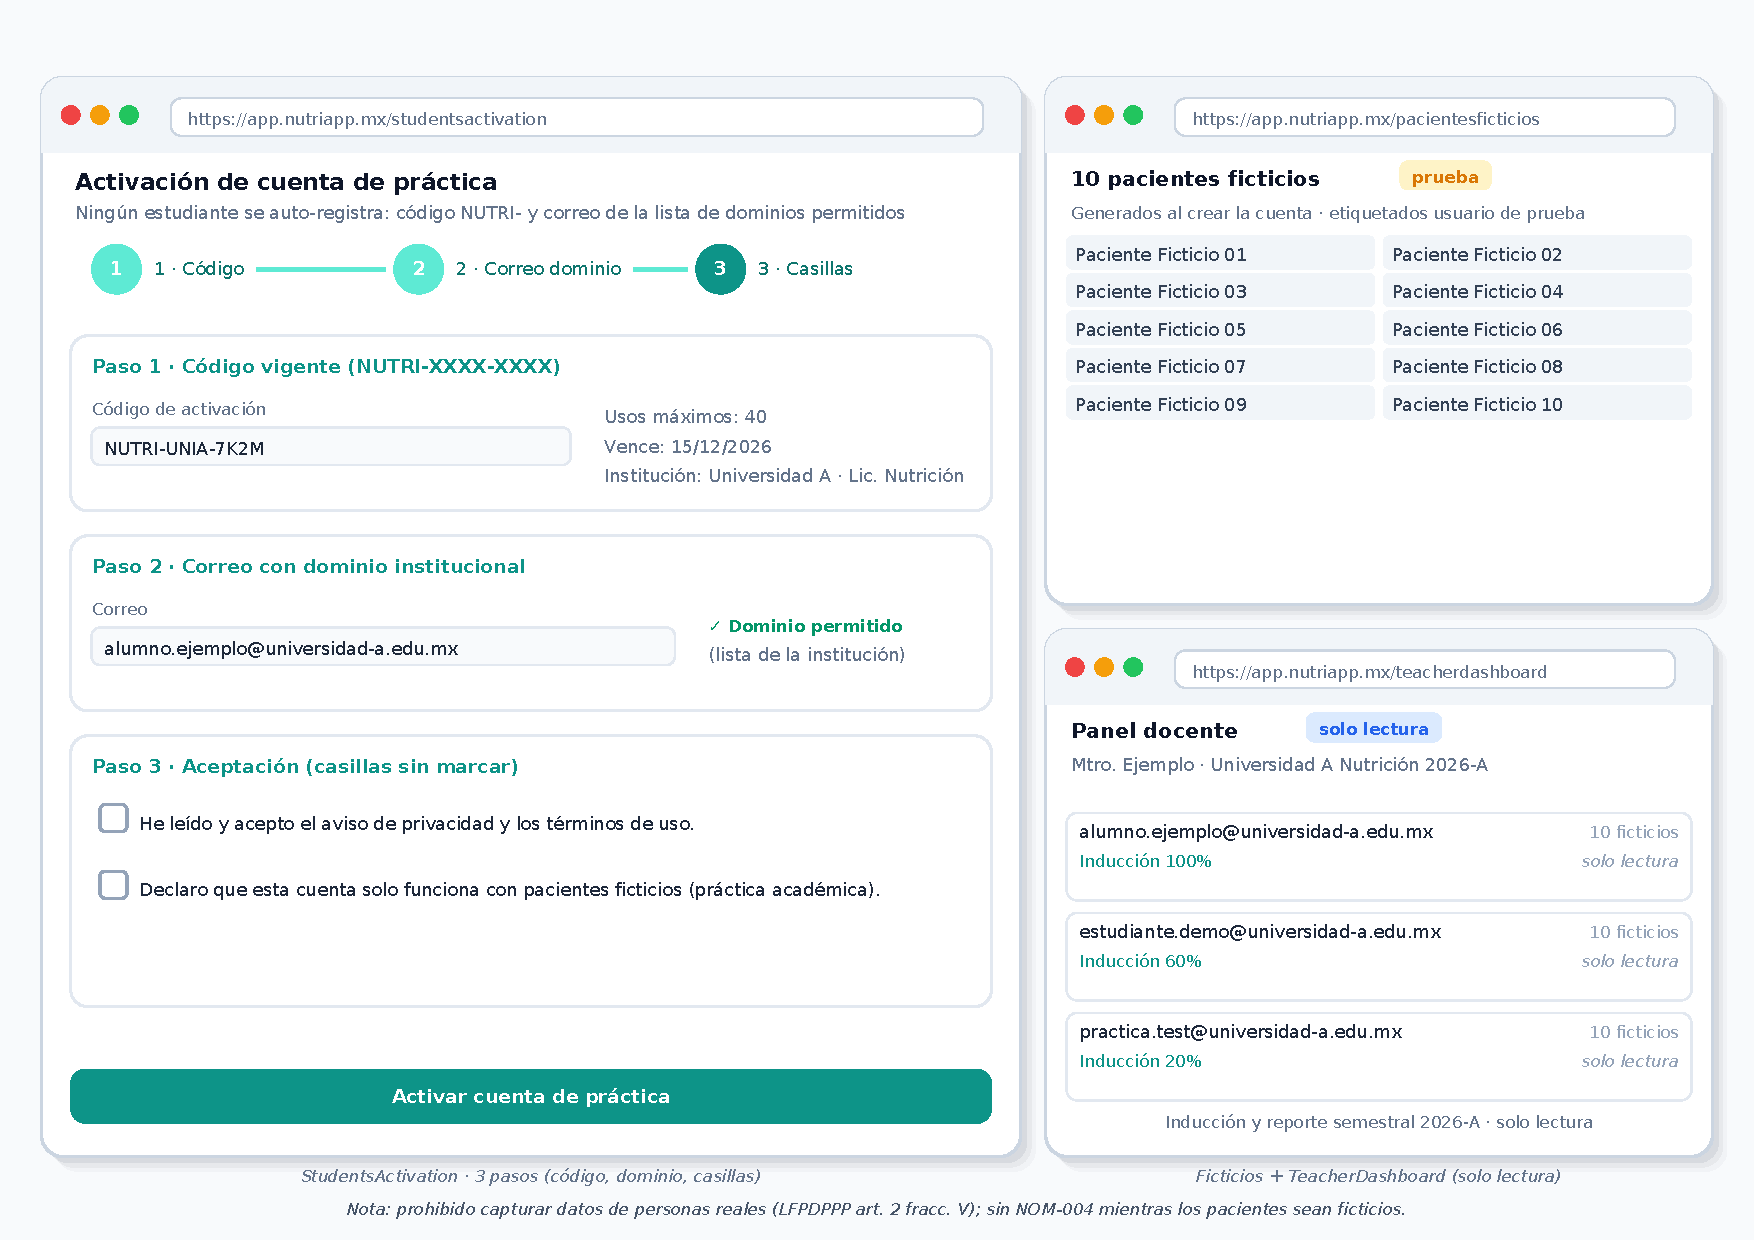
\includegraphics[width=\linewidth,height=0.88\textheight,keepaspectratio]{maqueta-students.pdf}
  \caption{Maqueta de la activación Students en tres pasos y del panel
  docente.}
  \label{fig:maq-students}
\end{figure}
\end{landscape}
 
\subsubsection{Comunidad y moderación}
 
\begin{sloppypar}
El módulo social permite al nutriólogo publicar contenido educativo, de
texto e imagen, visible para sus pacientes y para otros nutriólogos
(\texttt{SocialFeed}, \texttt{CreatePost}, \texttt{PostDetail}). La
responsabilidad por el contenido es del nutriólogo como profesionista
independiente y se establece en los términos de uso; NutriApp opera la
plataforma sin avalar lo publicado. El paciente o el nutriólogo pueden reportar
una publicación (\texttt{ReportContent}) y el administrador la revisa
en \texttt{AdminSocialModeration} con dos escalas: la publicación pasa
de \texttt{ACTIVE} a \texttt{HIDDEN} o \texttt{UNDER\_REVIEW}, y el
autor acumula \texttt{1ST\_STRIKE}, \texttt{2ND\_STRIKE} y
\texttt{SUSPENDED} por cada publicación ocultada, con
\texttt{UNDER\_REVIEW} cuando pide revisión, \texttt{REINSTATED} si
procede y \texttt{CANCELLED} cuando el administrador retira el módulo
social por reincidencia. La tercera amonestación suspende la
publicación durante treinta días, las amonestaciones caducan a los doce
meses, ninguno de estos estados afecta expedientes, citas ni
suscripción, y las imágenes admiten JPEG y PNG de hasta 5~MB. Toda
decisión genera un
folio \texttt{MOD-XXXXXXXX} en \texttt{moderation\_event} con motivo,
nota interna, fecha y hora, como registro de las decisiones tomadas.
\end{sloppypar}
 
% ─────────────────────────────────────────────────────────────────────────
\subsection{Prueba piloto: sesión y casos de prueba}
% ─────────────────────────────────────────────────────────────────────────
 
La prueba piloto
demuestra el diseño con usuarios sobre maquetas, sin llevarlo a
operación. La sesión sigue el procedimiento de la
sección~4.3.3; los casos de prueba se ejecutan aparte, como recorrido
sobre las maquetas (sección~4.4.2).
 
En la sesión, las maquetas se presentaron brevemente en pantalla con
perfiles de pacientes ficticios; las opiniones de los participantes
sobre ellas, previstas para el quinto bloque de la guía de discusión,
se recogieron con la encuesta de salida (secciones~4.3.3 y~7.1).
 
Los \textbf{casos de prueba de aceptación} siguen el formato de la
sección~4.4.2; la Tabla~\ref{tab:casos-prueba} los concreta para los
tres primeros flujos del MVP, y cada uno se califica en refleja, refleja
parcialmente o no refleja el diseño.
 
\begin{table}[H]
  \centering
  \caption{Casos de prueba de aceptación del MVP.}
  \label{tab:casos-prueba}
  \footnotesize
  \begin{tabularx}{\textwidth}{>{\raggedright\arraybackslash}p{2.1cm} X X X}
    \toprule
    \textbf{Caso} & \textbf{Obligación y precondición} & \textbf{Pasos} & \textbf{Resultado esperado y evidencia} \\
    \midrule
    CP-01 Consentimiento del paciente & LFPDPPP 2025, arts.~2, fracc.~IV, 8 y~15. Nutriólogo registrado con autenticación multifactor (MFA); paciente dado de alta con expediente «pendiente de consentimiento». & El paciente entra a su sesión, lee el aviso, marca la casilla obligatoria, deja la opcional sin marcar y confirma. & El expediente pasa de «pendiente de consentimiento» a activo; folio \texttt{DEC-} visible para ambos; el \texttt{DeclarationLog} muestra titular, mecanismo, versión del aviso, fecha y hora; ninguna casilla venía marcada. \\
    CP-02 Alta de paciente y expediente & LFPDPPP 2025, arts.~5 y~18; RLFPDPPP 2011, art.~48, fracc.~X. Consentimiento del CP-01 registrado. & El nutriólogo captura datos, una medición, una nota y un adjunto y asigna un plan en \texttt{AssignDiet}; el paciente lo consulta en \texttt{CurrentDiet}; un tercero sin relación intenta abrir el expediente. & El expediente admite los datos, la medición, la nota, el adjunto y el plan, que el paciente ve en \texttt{CurrentDiet}; cada acceso aparece en el registro que el paciente puede ver; el intento del tercero se rechaza y queda registrado. \\
    CP-03 Solicitud de cancelación & LFPDPPP 2025, arts.~24, 25, fracc.~VII, y~31; NOM-004-SSA3-2012, numeral~5.4. Expediente activo con datos. & El paciente solicita cancelación desde su perfil; el nutriólogo la resuelve dentro del plazo. & El diálogo explica veinte días para resolver y quince para ejecutar (art.~31), la conservación mínima y el bloqueo si procede; folio de la solicitud; la respuesta con folio llega al correo confirmado del titular y después se suprimen los datos de la cuenta y de contacto, salvo que el titular tenga otro expediente activo; el expediente queda en el estado que fije la resolución; aviso visible en la bandeja del nutriólogo. \\
    \bottomrule
  \end{tabularx}
\end{table}
 
% ─────────────────────────────────────────────────────────────────────────
\subsection{Justificación del alcance del MVP}
% ─────────────────────────────────────────────────────────────────────────
 
El alcance del MVP se definió con tres criterios. Por
\textit{completitud normativa}, deben estar presentes los módulos que
atienden las obligaciones de las Tablas~\ref{tab:trazabilidad-1}
y~\ref{tab:trazabilidad-2}: consentimiento, aviso de privacidad, ARCO, registro de
incidentes, inventario de datos, cifrado, MFA, trazabilidad y eliminación; las obligaciones
sanitarias ya declaradas
fuera del MVP no forman parte de ese criterio. La \textit{viabilidad
técnica} limita el MVP a lo que el diseño del capítulo~5 puede
sostener con Amazon Web Services (AWS) y React, con proveedores que son subcontrataciones
del encargado (Amazon SES, Twilio) o responsables independientes
(Mercado Pago) en los términos de la sección~5.1. La \textit{prioridad de uso} incluye los módulos
que un nutriólogo independiente usa a diario y que, por eso, los
participantes del grupo focal pueden juzgar con conocimiento de causa: gestión de
expedientes, agenda de citas y planes de alimentación.
 
Las maquetas navegables y el código del prototipo de interfaz están en el
repositorio del proyecto (NutriApp, 2026), y el Anexo~\ref{anexo:capturas} reproducirá las
pantallas principales. Antes de cualquier despliegue, el diseño tendría
que verificarse contra un catálogo de pruebas de seguridad de
aplicaciones, lo que se propone como siguiente paso en la
sección~8.3.
 
% ═══════════════════════════════════════════════════════════════════════════
\section{Resultados y análisis}
% ═══════════════════════════════════════════════════════════════════════════

% ─────────────────────────────────────────────────────────────────────────
\subsection{Evaluación del diseño con el grupo focal}
% ─────────────────────────────────────────────────────────────────────────
% NOTA: se completa después de la sesión del 23-oct-2026.
 
La evaluación sigue los tres métodos de la sección~4.4.2 y sus
resultados se leen contra la línea base del capítulo~3: lo que el
diagnóstico muestra ausente en la práctica reportada es lo que el
diseño debe resolver. En la aplicación, el quinto bloque de la guía no
llegó a desarrollarse: tras la demostración de las maquetas y tras el
cierre no hubo preguntas ni comentarios, de modo que la revisión por
expertos descansa en la encuesta de salida, que los ocho participantes
analizados respondieron entre el 25 y el 26 de octubre de 2026, dos y
tres días después de la sesión (Anexo~\ref{anexo:salida-resultados}).
 
\paragraph{Casos de prueba de aceptación}
\mbox{}
% Pendiente: resultado de CP-01, CP-02 y CP-03 (refleja / refleja
% parcialmente / no refleja), con la captura que sirve de evidencia en
% cada uno (Anexo B); los ejecuta y califica el autor (sección 4.4.3).
 
\paragraph{Revisión por expertos: la encuesta de salida}
Los ocho usarían las funciones mostradas y los ocho consideran
razonable el trabajo que la plataforma les pediría; la valoración se
respondió una sola vez para la lista completa de funciones, no función
por función. Solo dos dicen que lo mostrado se parece a cómo trabajan
hoy (cuatro respondieron «parcialmente» y dos «no»): el diseño no
replica la práctica actual y aun así lo usarían. Los ocho perciben el
código de verificación al iniciar sesión y el folio de cada
consentimiento o solicitud como una protección y no como un trámite
extra. Siete aceptarían ---y uno respondió «tal vez»--- que, ante la
petición de borrar toda la información, la plataforma bloquee el
expediente clínico en lugar de borrarlo y les indique qué responder y
en qué plazo: es la respuesta del diseño al hallazgo del diagnóstico
(sección~3.3). Las dos funciones que no se mostraron se preguntaron
descritas: los ocho creen que la cuenta de práctica ayudaría a que los
estudiantes aprendan lo que pide la ley, y los ocho aparecerían en el
catálogo con reserva de cita.
 
En las respuestas abiertas, cinco señalan como lo más útil funciones de
cumplimiento (el seguimiento legal por paciente, la orientación sobre
qué responder a quien pide borrar su información, la depuración a los
cinco años, el orden de los apartados) y tres, funciones de gestión de
la consulta (finanzas, agenda y vista del paciente con confirmación de
citas). Las mejoras pedidas fueron un diseño visual más amigable (tres
menciones); el tratamiento de pacientes menores de edad ---indicar que
el consentimiento lo firmó el tutor y adaptar los flujos a la consulta
pediátrica, dos menciones que se recogen como siguiente paso en la
sección~8.3---; conservar plantillas propias (una); y que el paciente
agende directamente (una), función que el diseño ya prevé en el
catálogo (sección~6.2.4) y que esa participante valoró como motivo para
dejar la plataforma comercial que hoy usa como agenda y directorio.
Siete piensan cambiar algo en su práctica a partir de la sesión y uno
respondió «tal vez»; lo primero que harían coincide con las ausencias
del diagnóstico: entregar un aviso de privacidad por escrito (siete),
pedir el consentimiento para datos de salud aparte del clínico (seis) y
definir la conservación de cinco años (cuatro). Estas respuestas se
leen como evidencia exploratoria de la revisión por expertos, no como
prueba de uso: los participantes evaluaron una demostración, no
operaron las maquetas; conocían al autor, recibieron un pago y el
formulario registró su nombre, condiciones que favorecen la
complacencia; y la encuesta se respondió días después de la sesión, por
lo que recoge lo que los participantes declaran tras ese intervalo
(sección~8.3).
 
\paragraph{Observación en el caso}
La hoja de observación prevista para el quinto bloque quedó sin
materia, porque no hubo discusión sobre las maquetas. Lo observado se
reduce a tres hechos. El primero es el propio silencio tras la
demostración y tras el cierre. El segundo, durante los bloques de
práctica, fue el interés en que la herramienta avise cuándo depurar
expedientes («yo creo que me serviría», ante la pregunta del
moderador). El tercero fue el relato de una participante que dejó un
software comercial porque el personal del proveedor podía acceder a la
información de sus pacientes. Los dos últimos sostienen decisiones ya
tomadas en el diseño: los avisos de vencimiento de la conservación con
confirmación del responsable (sección~2.5.5) y la transparencia de las
subcontrataciones ante el nutriólogo (sección~5.1).
 

% ─────────────────────────────────────────────────────────────────────────
\subsection{Validación normativa del diseño propuesto}
% ─────────────────────────────────────────────────────────────────────────

La validación normativa del diseño de NutriApp consiste en verificar
que cada obligación legal identificada en las Tablas~\ref{tab:trazabilidad-1}
y~\ref{tab:trazabilidad-2} tiene un componente técnico correspondiente en el
diseño de los capítulos~5 y~6; esa correspondencia se sintetiza por
capa (Tabla~\ref{tab:stack}) y la lista siguiente la completa obligación
por obligación. El
criterio de validez es la completitud respecto de las obligaciones de
esas dos tablas, con las exclusiones sanitarias que declara la
sección~6.1; no se afirma completitud sobre la totalidad de la
Ley Federal de Protección de Datos Personales en Posesión de los Particulares (LFPDPPP) 2025, su Reglamento, la NOM-004-SSA3-2012 o la
NOM-024-SSA3-2012.
 
El análisis de trazabilidad recorre las once obligaciones de las
tablas, con sus mismos rótulos y en su mismo orden, y encuentra para
cada una el componente que la atiende:
 
\begingroup\sloppy
\begin{enumerate}[label=\Roman*.]
  \item Consentimiento expreso por escrito para datos de salud
    (LFPDPPP, 2025, art.~8): pantalla de
    consentimiento del paciente (sección~6.2.1, caso CP-01) con folio
    \texttt{DEC-} y fecha y hora inmutables en el \texttt{DeclarationLog}.
  \item Aviso de privacidad previo al tratamiento (LFPDPPP, 2025,
    arts.~14 y~15): plantilla que el nutriólogo completa y valida como
    responsable, presentada al paciente antes de capturar cualquier dato,
    con registro de la versión aceptada; accesible desde cualquier
    pantalla.
  \item Medidas de seguridad técnicas y administrativas (LFPDPPP, 2025,
    art.~18; Reglamento de la Ley Federal de Protección de Datos Personales en Posesión de los Particulares [RLFPDPPP], 2011, art.~57): cifrado AES-256 (Advanced Encryption Standard) en reposo y TLS~1.3 (Transport Layer Security) en
    tránsito, autenticación multifactor (MFA), control de acceso por rol, registros de auditoría y
    separación de entornos.
  \item Autenticación verificable de usuarios (NOM-024-SSA3-2012, 2012,
    numeral~6.6.3): Amazon Cognito con MFA por código TOTP, obligatoria
    para el nutriólogo, el docente y el administrador y opcional para el
    paciente.
  \item Trazabilidad de consultas, accesos y modificaciones (LFPDPPP, 2025,
    art.~13; RLFPDPPP, 2011, art.~48, fracc.~X): CloudTrail, pgAudit y la capa de aplicación
    (\texttt{DeclarationLog} y \texttt{audit\_log}), exportados a S3 con
    Object Lock y conservados cinco años.
  \item Inventario de datos, análisis de riesgos y análisis de brecha
    (RLFPDPPP, 2011, art.~61): inventario de datos versionado, en JSON y
    PDF, generado a partir del modelo de datos y clasificado por nivel
    de sensibilidad, entregado al nutriólogo como insumo de su propio
    análisis (sección~5.1).
  \item Gestión de derechos ARCO en plazo legal (derechos de acceso, rectificación, cancelación y oposición; LFPDPPP, 2025,
    art.~31): módulo ARCO con fechas límite calculadas y avisos
    automáticos de vencimiento en la aplicación y por correo; la
    resolución la emite el nutriólogo.
  \item Aviso al titular ante vulneraciones de seguridad (LFPDPPP, 2025,
    art.~19; RLFPDPPP, 2011, arts.~64 y~65): registro de incidentes con alerta
    al nutriólogo, que decide y envía el aviso; la plataforma asienta
    fecha, alcance y acciones con folio.
  \item Confidencialidad y conservación del expediente clínico
    (LFPDPPP, 2025, arts.~24 y~25; NOM-004-SSA3-2012, 2012, numeral~5.4):
    expediente en RDS sin operación de borrado durante la retención;
    adjuntos y registros en S3 con Object Lock; al vencer la retención o
    el bloqueo, aviso programado al nutriólogo, confirmación del
    responsable y destrucción criptográfica por Lambda, que queda con
    folio en el registro de auditoría.
  \item Autenticación, perfiles de acceso y trazabilidad en sistema
    de expediente clínico electrónico (NOM-024-SSA3-2012, 2012, numerales~6.6.1,
    6.6.3 y~6.6.4): atendidos con Cognito, control por rol y las tres
    capas de auditoría; la MFA y el cifrado con llaves en AWS Key Management Service (KMS) exceden lo
    que la norma pide. El numeral~6.6.5 no resulta aplicable porque el producto mínimo viable (MVP) no
    intercambia información entre prestadores; la firma electrónica
    avanzada (numeral~6.6.2) y la exportación (numeral~6.6.6) quedan
    fuera del MVP (sección~6.1).
  \item Uso de proveedor de cómputo en la nube (RLFPDPPP, 2011, arts.~51,
    52 y~54): NutriApp como encargado bajo contrato con el nutriólogo;
    AWS (incluido Amazon SES, en \texttt{us-east-1}) y Twilio
    como subcontrataciones autorizadas y
    transparentadas.
\end{enumerate}
\endgroup
 
De las debilidades de la ley que examina la sección~2.3.2, la ausencia
de portabilidad de datos como derecho explícito en la LFPDPPP no puede
resolverse por diseño técnico; requiere reforma legal. La exportación
estructurada del expediente en formato transferible, que la NOM-024 prevé
para el sistema (numeral~6.6.6), queda fuera del MVP y se
propone como siguiente paso en la sección~8.3.

% ─────────────────────────────────────────────────────────────────────────
\subsection{Costo de operar el diseño y relación costo-beneficio}
\label{sec:costos}
% ─────────────────────────────────────────────────────────────────────────
 
El análisis costo-beneficio compara el costo anual que pagaría el nutriólogo por el
plan Pro, según la propuesta de precios de la sección~8.3.1, con la magnitud de las sanciones que enfrenta un
nutriólogo independiente por incumplir la LFPDPPP~2025.
 
Lo que sigue es una estimación de referencia para quien implemente el
diseño, no la contabilidad de un servicio en operación: el caso termina
en el diseño y la prueba piloto, y estas cifras estiman lo que costaría
llevarlo a la práctica.
 
\textbf{Modelo de carga.} Antes de estimar costos hay que saber cuánto
trabajo real recibe la plataforma, porque la mayor parte del costo de los
servicios del capítulo~5 es fijo, por hora o por mes, y solo unos
cuantos componentes crecen con el tráfico. El dimensionamiento supuesto para el MVP, 500 nutriólogos y
5,000 pacientes, se traduce en solicitudes (Tabla~\ref{tab:carga}): con seis consultas diarias por
nutriólogo, treinta llamadas a la API por consulta y seis sesiones
mensuales por paciente, el sistema atendería 2.2 millones de solicitudes al
mes, que en la hora hábil media son 3.5 por segundo y en la hora pico
(tres veces la media) 10.5 por segundo. Con funciones de 200 milisegundos,
eso equivale a dos ejecuciones simultáneas de Lambda. La ruta crítica eleva
las consultas a 1.5 veces, las llamadas por consulta a cuarenta y las
sesiones del paciente al doble, con un pico de cinco veces la media, y
aun así queda en 36
solicitudes por segundo y once ejecuciones simultáneas. Los límites de
referencia son de otro orden: mil ejecuciones simultáneas por cuenta en
Lambda, 2,500 solicitudes por segundo en API Gateway para la región de
México y unas 225 conexiones en una instancia db.t4g.small (AWS,
s.f.-f). No hay, en ningún escenario, transacciones simultáneas
que la instancia o las funciones no puedan atender; lo que encarece la
ruta crítica son los componentes que cobran por mensaje.
 
\begin{table}[H]
  \centering
  \caption{Modelo de carga del MVP: de usuarios a solicitudes por segundo.}
  \label{tab:carga}
  \footnotesize
  \begin{tabularx}{\textwidth}{X r r}
    \toprule
    \textbf{Variable} & \textbf{Base} & \textbf{Ruta crítica} \\
    \midrule
    Consultas por nutriólogo por día & 6 & 9 \\
    Solicitudes a la API por consulta & 30 & 40 \\
    Sesiones mensuales por paciente (8 / 10 solicitudes) & 6 & 12 \\
    Consultas al mes & 66,000 & 99,000 \\
    Solicitudes a la API al mes (millones) & 2.2 & 4.6 \\
    Solicitudes por segundo, hora hábil media & 3.5 & 7.2 \\
    Factor de hora pico & 3$\times$ & 5$\times$ \\
    Solicitudes por segundo en hora pico & 10.5 & 36.0 \\
    Ejecuciones Lambda simultáneas en hora pico (200 / 300 ms) & 2.1 & 10.8 \\
    Mensajes con efecto jurídico al mes (acuse de consentimiento, respuestas ARCO e incidentes) & 540 & 2,700 \\
    \midrule
    \textit{Límites de referencia:} Lambda 1,000 simultáneas; API Gateway 2,500 req/s (mx-central-1); RDS db.t4g.small $\approx$ 225 conexiones & & \\
    \bottomrule
  \end{tabularx}
\end{table}
 
\textbf{Costo operativo en dos escenarios.} La Tabla~\ref{tab:costos}
estima el costo mensual con ese modelo de carga y con las reglas de la
Tabla~\ref{tab:costos-reglas}. La columna «varía» dice si el componente
crece con la carga: los que cobran por hora (instancia de base de
datos, NAT Gateway, punto de enlace) cuestan
lo mismo con dos o con once ejecuciones simultáneas; los que cobran por
solicitud o por mensaje (API Gateway, CloudTrail, WhatsApp, mensajes de texto [SMS]) son los
que forman la ruta crítica. Los precios son de lista, consultados en
septiembre de 2026 (AWS, s.f.-e; Mercado
Pago, s.f.-b; Meta, 2025; Twilio, 2026); las tarifas de mx-central-1, publicadas en los archivos de
la Price List de AWS (AWS, s.f.-g), se aproximan con las de us-east-1 y
un factor regional del 5\% (regla R2).
 
El escenario base cuesta \$141 dólares al mes (\$1,692 dólares al año; \$0.28 dólares por
nutriólogo activo) y la ruta crítica \$299 dólares (\$3,588 dólares al año; \$0.60 dólares). La
diferencia, \$158 dólares, se concentra en la mensajería (SMS de respaldo,
\$88 dólares más; WhatsApp, \$22 dólares más) y en API Gateway con CloudTrail (\$24 dólares
más). El SMS en
México cuesta \$0.1819 dólares por mensaje (Twilio, 2026) frente a \$0.013 dólares del
mensaje de utilidad de WhatsApp, por lo que el diseño lo reserva para el
paciente sin WhatsApp y solo para avisos con efecto jurídico (regla R3);
las citas se notifican dentro de la aplicación. La alta disponibilidad
(base de datos en dos zonas, NAT y punto de enlace redundantes) es una
decisión de servicio, independiente de la carga, y por eso se
muestra aparte: \$67 dólares al mes con el factor regional.
 
\begin{table}[H]
  \centering
  \caption{Estimación de costos operativos en dos escenarios (500 nutriólogos
  activos, 5,000 pacientes; USD por mes).}
  \label{tab:costos}
  \scriptsize
  \setlength{\tabcolsep}{3pt}
  \renewcommand{\arraystretch}{1.05}
  \begin{tabularx}{\textwidth}{p{3.4cm} c X r r}
    \toprule
    \textbf{Componente} & \textbf{Varía} & \textbf{Base de cálculo (base / ruta crítica)} & \textbf{Base} & \textbf{Crít.} \\
    \midrule
    CloudFront + S3 (sitio) & sí & 21 / 65~GB, capa gratuita permanente & \$1 & \$1 \\
    WAF + Shield Standard & parcial & 2 ACL y 4 reglas fijas cada una; 2.2 / 4.6~M solicitudes & \$19 & \$21 \\
    API Gateway + Lambda & sí & 2.2 / 4.6~M solicitudes; Lambda dentro / fuera de capa gratuita & \$8 & \$21 \\
    Amazon Cognito & no & 5,500 usuarios activos mensuales (MAU); Essentials, 10,000 gratuitos & \$0 & \$0 \\
    RDS PostgreSQL (db.t4g.small) & parcial & instancia en una zona; 20 / 40~GB, más 20~GB de respaldo en la ruta crítica & \$26 & \$30 \\
    NAT Gateway & parcial & 1 zona; salida hacia Amazon SES, Twilio y Mercado Pago & \$33 & \$33 \\
    Puntos de enlace privados & no & S3 por gateway (sin costo); KMS por interfaz & \$8 & \$8 \\
    KMS + ACM & parcial & 1 / 2 llaves; una llamada por cada dos solicitudes & \$4 & \$9 \\
    S3 (adjuntos y registros) & sí & 50 / 150~GB acumulados y solicitudes; Object Lock sin cargo & \$3 & \$8 \\
    CloudTrail + CloudWatch & sí & un evento de datos por solicitud; 5 / 15~GB de logs y 4.4 / 9.1~GB de pgAudit (R6) & \$7 & \$18 \\
    EventBridge + Lambda (avisos y supresión confirmada) & no & capa gratuita permanente & \$0 & \$0 \\
    Route 53 & parcial & zona fija + consultas & \$1 & \$2 \\
    \midrule
    \textit{Subtotal AWS (us-east-1)} & & & \$111 & \$152 \\
    Factor regional (R2) & no & 5\% sobre el subtotal AWS & \$6 & \$8 \\
    Dominio (anual prorrateado) & no & .com / .com y .mx & \$1 & \$7 \\
    Twilio: WhatsApp (R3) & sí & 486 / 2,160 mensajes de utilidad a \$0.013 & \$6 & \$28 \\
    Twilio: SMS de respaldo (R3) & sí & 54 / 540 mensajes a \$0.1819 + número local (\$6.50 al mes) & \$16 & \$105 \\
    \midrule
    \textbf{Total mensual} & & & \textbf{\$141} & \textbf{\$299} \\
    \textbf{Total anual} & & & \textbf{\$1,692} & \textbf{\$3,588} \\
    \textbf{Por nutriólogo activo al mes} & & & \textbf{\$0.28} & \textbf{\$0.60} \\
    \midrule
    \textit{Opción: alta disponibilidad (no incluida)} & opción & RDS Multi-AZ, NAT y punto de enlace en 2.ª zona, con factor regional & \$67 & \$67 \\
    \bottomrule
  \end{tabularx}
  \begin{flushleft}
    \footnotesize\textit{Nota.} Precios de lista sin instancias reservadas (con
    reserva de un año, RDS baja cerca de un 30\%). Cifras redondeadas al
    dólar; el total mensual se calcula sin redondear y el anual es el
    total mensual por doce. El costo de Mercado Pago es una comisión sobre cada cobro, no infraestructura (Tabla~\ref{tab:ingresos}).
    La hoja de cálculo con precios, supuestos y
    fórmulas es un archivo de trabajo del autor, disponible a solicitud.
  \end{flushleft}
\end{table}
 
\begin{table}[H]
  \centering
  \caption{Reglas de estimación de los dos escenarios de costo.}
  \label{tab:costos-reglas}
  \footnotesize
  \begin{tabularx}{\textwidth}{l X}
    \toprule
    \textbf{Regla} & \textbf{Enunciado} \\
    \midrule
    R1 Carga & Los volúmenes salen del modelo de la Tabla~\ref{tab:carga}, no de multiplicadores fijos, con 22 días hábiles al mes y ocho horas hábiles por día. La ruta crítica es el mes de mayor actividad plausible con los mismos usuarios: 1.5 veces las consultas, pico de cinco veces la hora media, el doble de pacientes nuevos y cuatro veces las solicitudes ARCO. No supone crecimiento de usuarios. \\
    R2 Región & Los precios de mx-central-1 se estiman como los de us-east-1 más 5\%, diferencial observado en cómputo de propósito general entre ambas regiones (aws-pricing.com, 2026); se sustituye por la tarifa exacta de la calculadora de AWS al presupuestar. \\
    R3 Mensajería & El canal por defecto de todo aviso es el correo confirmado de la cuenta (Amazon SES, costo marginal). Twilio se usa solo para avisos con efecto jurídico (acuse de consentimiento, respuestas ARCO, incluida la de una cancelación con su periodo de bloqueo, e incidentes), con dos mensajes por evento en la base y tres en la ruta crítica, al 60 / 90\% de pacientes que aceptan la casilla de avisos, sobre unos 450 / 1,000 eventos al mes (pacientes nuevos y solicitudes ARCO). WhatsApp con plantillas de utilidad es el canal principal; el SMS cubre al 10 / 20\% que no tiene WhatsApp. Las citas se notifican dentro de la aplicación. Ningún factor de autenticación viaja por SMS. \\
    R4 Disponibilidad & Ambos escenarios usan RDS en una zona con respaldo continuo. Multi-AZ, NAT y punto de enlace en segunda zona son una opción de servicio que se cotiza aparte (\$67 al mes). \\
    R5 Salida a internet & Las funciones dentro de la VPC salen a Amazon SES, Twilio y Mercado Pago por NAT Gateway; se estima que el 10\% del tráfico de la API cruza el NAT. S3 se alcanza por punto de enlace de gateway (sin costo) y KMS por interfaz. \\
    R6 Auditoría & pgAudit (\texttt{pgaudit.log = 'read, write, ddl'}, sin registrar parámetros) publica en CloudWatch Logs 2~KB por solicitud a la API, y una tarea periódica lo exporta a S3; CloudTrail registra un evento de datos por solicitud además del trail de administración gratuito. \\
    R7 Identidad & Cognito Essentials: 10,000 usuarios activos mensuales sin costo; el MVP no los alcanza en ningún escenario. \\
    R8 Dominio & .com en Route 53 en la base; .com y .mx en la ruta crítica. Precio anual, variable por registrador, prorrateado a doce meses. \\
    R9 Cobros & La comisión de Mercado Pago es costo variable sobre el ingreso (Tabla~\ref{tab:ingresos}), no infraestructura. \\
    R10 Capas gratuitas & Solo las permanentes (Lambda, CloudFront, EventBridge, primer trail de CloudTrail), no las de doce meses. \\
    R11 Vigencia & Precios de lista del 24 de septiembre de 2026; se revisan al presupuestar cada fase. \\
    \bottomrule
  \end{tabularx}
\end{table}
 
\textbf{Inversión inicial.} El costo operativo supone que el sistema ya
existe. La Tabla~\ref{tab:inversion} estima lo que cuesta llevar el
diseño de este trabajo a un producto en operación, sin mercadotecnia. Dos
rubros son tarifas oficiales: la constitución de una Sociedad por
Acciones Simplificada (SAS), que es gratuita en línea (Secretaría de Economía,
s.f.), y el estudio de la solicitud de registro de marca, que cuesta
\$2,695.18 pesos más el impuesto al valor agregado, o IVA (Instituto
Mexicano de la Propiedad Industrial [IMPI], 2023), y el dominio es precio de lista de Route~53. El resto son
estimaciones del autor con rango, y el desarrollo domina: ochocientas
horas para convertir las maquetas en el sistema descrito en los
capítulos~5 y~6, a tarifas de mercado de entre \$300 y \$500 pesos
por hora. Si el propio autor construye el MVP, la inversión en efectivo
baja a entre \$63,000 y \$148,000 pesos.
 
\begin{table}[H]
  \centering
  \caption{Inversión inicial estimada, sin mercadotecnia (MXN).}
  \label{tab:inversion}
  \footnotesize
  \begin{tabularx}{\textwidth}{X l r r}
    \toprule
    \textbf{Concepto} & \textbf{Tipo} & \textbf{Mínimo} & \textbf{Máximo} \\
    \midrule
    Constitución de la sociedad (SAS en línea) & tarifa & \$0 & \$0 \\
    Registro de marca ante el IMPI, una clase (sin IVA) & tarifa & \$2,695 & \$2,695 \\
    Aviso de privacidad, términos de uso y contratos con encargados & estimación & \$15,000 & \$40,000 \\
    Alta fiscal y contabilidad del primer trimestre & estimación & \$6,000 & \$12,000 \\
    Desarrollo del MVP a partir de las maquetas (800~h) & estimación & \$240,000 & \$400,000 \\
    Pruebas de seguridad (prueba de penetración básica) & estimación & \$25,000 & \$60,000 \\
    Constancias NOM-151-SCFI-2016 con un prestador de servicios de certificación & estimación & \$5,000 & \$15,000 \\
    Dominio, primer año & tarifa & \$288 & \$1,494 \\
    Herramientas de diseño y colaboración, doce meses & estimación & \$3,500 & \$7,000 \\
    Ambiente AWS de desarrollo y pruebas, tres meses & estimación & \$6,000 & \$10,000 \\
    \midrule
    \textbf{Total} & & \textbf{\$303,000} & \textbf{\$548,000} \\
    Equivalente en USD (18 pesos por dólar) & & \$16,900 & \$30,500 \\
    Sin el desarrollo, si el autor construye el MVP & & \$63,000 & \$148,000 \\
    \bottomrule
  \end{tabularx}
\end{table}
 
\textbf{Magnitud de las sanciones previstas.} La LFPDPPP~2025 establece
sanciones de hasta 320,000 veces la Unidad de Medida y Actualización (UMA) por
las infracciones del art.~58, fraccs.~VIII a~XVIII (LFPDPPP, 2025, art.~59, fracc.~III). Con el valor de la
UMA~2025 de \$113.14 pesos diarios (Instituto Nacional de Estadística y Geografía [INEGI], 2025), el techo de una multa
por esas infracciones es de \$36,204,800 pesos, que puede incrementarse hasta por dos veces,
a \$72,409,600 pesos, cuando involucra datos sensibles de salud (LFPDPPP,
2025, art.~59, fracc.~IV). En la práctica, el último balance anual de
multas que el Instituto Nacional de Transparencia, Acceso a la Información y Protección de Datos Personales (INAI) difundió por comunicado antes de su extinción
corresponde a 2023: multas por un
total de \$46,849,777 pesos y 74 procedimientos de imposición de
sanciones concluidos (INAI, 2024), lo que dio una multa promedio
impuesta de unos \$633,105 pesos por procedimiento concluido. La cifra
describe multas impuestas, no cobradas: en enero de 2026 la Secretaría Anticorrupción y Buen Gobierno (SABG) informó
que halló procedimientos del extinto INAI reportados indebidamente como
concluidos y resoluciones sancionatorias cuya ejecución se omitió, lo
que impidió cobrar las multas (SABG, 2026). No se localizaron
estadísticas de sanciones de la SABG publicadas antes del corte de
enero de 2026.
 
La comparación (Tabla~\ref{tab:costo-beneficio}) muestra el orden de magnitud: la multa promedio que impuso
el INAI en 2023 equivale a 181 veces el costo del plan Pro anual de
NutriApp (\$3,490 pesos); el techo de multa que puede alcanzarse con el
incremento por datos sensibles, a 20,748 veces. La disyuntiva para el
nutriólogo independiente es, por tanto, entre un costo cierto y pequeño y un
riesgo poco frecuente según las cifras del INAI (INAI, 2024), pero desproporcionado;
la suscripción no sustituye el cumplimiento, que sigue siendo del nutriólogo.
 
\begin{table}[H]
  \centering
  \caption{Análisis costo-beneficio: NutriApp Pro frente a las sanciones de la LFPDPPP~2025.}
  \label{tab:costo-beneficio}
  \begin{tabularx}{\textwidth}{X r r}
    \toprule
    \textbf{Concepto} & \textbf{MXN} & \textbf{Factor} \\
    \midrule
    Suscripción NutriApp Pro, plan anual (IVA incluido) & \$3,490 & 1$\times$ \\
    Multa promedio impuesta por el INAI en 2023 (por procedimiento concluido) & \$633,105 & 181$\times$ \\
    Techo de multa por las infracciones del art.~58, fraccs.~VIII a~XVIII (art.~59, fraccs.~III y~IV), con incremento por datos sensibles (por infracción) & \$72,409,600 & 20,748$\times$ \\
    Honorarios de defensa legal (estimación) & \$150,000--\$300,000 & 43--86$\times$ \\
    \bottomrule
  \end{tabularx}
  \begin{flushleft}
    \small\textit{Nota.} Multa promedio impuesta, calculada sobre el total
    de multas que el INAI impuso en 2023 (\$46,849,777 pesos) entre 74
    procedimientos concluidos (INAI, 2024). Los honorarios de defensa legal
    son estimaciones de mercado; no constituyen asesoría jurídica. Con base en LFPDPPP (2025), INAI (2024) e INEGI (2025).
  \end{flushleft}
\end{table}

% ═══════════════════════════════════════════════════════════════════════════
\section{Conclusiones}
% ═══════════════════════════════════════════════════════════════════════════

\subsection{Hallazgos frente a las preguntas guía}
Las cinco preguntas de la sección~1.5 ordenan los hallazgos.

La primera pedía identificar las obligaciones que el marco mexicano
impone al nutriólogo de consulta privada y lo que deja sin precisar
frente a Brasil, Uruguay, Estados Unidos y Alemania. El capítulo~2
identificó once obligaciones exigibles, del aviso de privacidad a las
condiciones del cómputo en la nube (Tablas~\ref{tab:trazabilidad-1}
y~\ref{tab:trazabilidad-2}), y las imprecisiones que la comparación
hace visibles: la ley mexicana no dice qué medidas de seguridad bastan,
no fija plazo para avisar una vulneración ni obliga a notificarla a la
autoridad, y deja fuera la portabilidad; el expediente clínico
electrónico no es obligatorio, de modo que la NOM-024 solo alcanza a
quien adopta un sistema electrónico.

La segunda preguntaba qué obligaciones están presentes y cuáles
ausentes en la práctica reportada, y por qué. En el grupo estudiado
están parcialmente presentes las medidas básicas de seguridad y el
conocimiento del propio inventario, y ausentes el aviso de privacidad
sistemático, el consentimiento específico para datos de salud, la
trazabilidad de accesos, el procedimiento ante vulneraciones, la
gestión de solicitudes con plazo y registro, y la regla de conservación
aplicada, que se conoce más de lo que se practica. Las razones
reportadas son el desconocimiento operativo de la ley y herramientas
que no incorporan esas funciones, no el rechazo a la obligación
(sección~3.3).

La tercera preguntaba si un diseño de software puede convertir esas
obligaciones en funciones verificables sin asumir las decisiones que la
ley reserva al profesional. En el nivel del diseño, la respuesta es
afirmativa: la matriz de trazabilidad liga cada obligación con un
componente comprobable (sección~7.2) y las decisiones quedan en el
nutriólogo ---resolver cada solicitud, negar una cancelación con
fundamento, confirmar la supresión, decidir y enviar el aviso ante una
vulneración---, mientras la plataforma aporta los medios y deja
constancia con folio. La comprobación se hizo sobre maquetas; su
verificación en un sistema en ejecución queda para la fase de
desarrollo (sección~8.3).

La cuarta preguntaba cómo valoran esas funciones nutriólogos con
práctica clínica frente a su forma actual de trabajo. Los ocho
participantes analizados usarían las funciones mostradas, consideran
razonable la carga de trabajo y perciben el folio y el código de acceso
como protección; siete aceptarían el bloqueo en lugar del borrado ante
una solicitud de cancelación; y solo dos dicen que el diseño se parece
a cómo trabajan hoy, lo que confirma la distancia entre la práctica y
la norma que el diseño busca cerrar. La evidencia es exploratoria, en
los términos de las secciones~7.1 y~8.3.

La quinta preguntaba cuánto costaría operar el diseño y cómo se compara
la suscripción con las sanciones. Operar el producto mínimo viable para
500 nutriólogos y 5,000 pacientes costaría entre \$141 y \$299 dólares
al mes según el escenario, de \$0.28 a \$0.60 dólares por nutriólogo;
la multa promedio que impuso el INAI en 2023 equivale a 181
suscripciones anuales del plan Pro y la sanción máxima con datos de
salud a 20,748, una comparación que encuadra el costo como fracción
menor del riesgo sin presentar la suscripción como sustituto del
cumplimiento, que sigue siendo del nutriólogo (sección~7.3).

\subsection{Lecciones aprendidas y recomendaciones para el gremio}
La lección central del caso es que la brecha de cumplimiento en la
consulta de nutrición es operativa, no actitudinal. Los participantes
protegen la disponibilidad de su información ---contraseñas, respaldos,
nube--- porque sus herramientas lo facilitan; no entregan aviso de
privacidad, no separan el consentimiento de datos del clínico y no
registran accesos ni plazos porque nadie se los enseñó y porque sus
herramientas no lo traen. Quien quiera cerrar la brecha tiene que
atacar el desconocimiento y la herramienta a la vez; la sola difusión
de la norma deja al profesional sabiendo qué debe, sin con qué.

Del diagnóstico se siguen prácticas que no requieren software y que el
gremio puede adoptar de inmediato: entregar un aviso de privacidad por
escrito con los elementos del artículo~15 de la ley; recabar el
consentimiento para los datos de salud por separado del consentimiento
clínico y conservar la constancia; fijar la regla de conservación de
cinco años con una depuración programada, que alcance también a los
respaldos; anotar con fechas toda solicitud de un paciente sobre sus
datos; tener por escrito tres pasos ante un incidente ---contener,
documentar y avisar al titular sin dilación---; y revisar dónde guarda
los datos el proveedor de software o de nube y bajo qué condiciones,
antes de contratarlo. El documento de referencia entregado a los
participantes (Anexo~\ref{anexo:referencia}) resume estas prácticas
con su fundamento normativo.

Para las instituciones que forman nutriólogos, el caso aporta dos
datos: ninguna norma de educación superior exige la protección de datos
como contenido específico de la carrera (sección~3.1) y cuatro de los
ocho participantes no han recibido formación alguna en la materia,
mientras el cierre de la sesión mostró que una exposición breve y
situada en el consultorio basta para que el profesional identifique qué
le falta. Incorporar el manejo legal del expediente a los planes de
estudio no requiere una asignatura nueva: cabe en las materias de
ética, de tecnología o de práctica profesional ya existentes. La cuenta
de práctica para estudiantes del diseño (sección~6.2.5) y el Plan
Universidad (sección~8.3.1) se proponen como una vía, no como un
resultado.

Para quienes desarrollan software para el sector, el hallazgo es que
usar una herramienta especializada hoy no se traduce en cumplimiento:
en el grupo, las obligaciones ausentes lo están por igual entre quienes
usan software comercial y quienes usan archivos de uso general, y «mi
herramienta no lo trae» apareció como obstáculo declarado. Incorporar
el aviso, el consentimiento con constancia, los plazos y el registro de
accesos es una oportunidad de diferenciación además de una necesidad
regulatoria; el paquete de diseño de este caso documenta una forma de
hacerlo.

\subsection{Limitaciones, siguientes pasos y transferencia del diseño}
El caso se limita al diseño y a su demostración: el análisis normativo
del capítulo~2, el diagnóstico del capítulo~3, el paquete de
diseño del capítulo~5 y las maquetas con su prueba piloto del
capítulo~6. No incluye la implementación productiva de NutriApp, su
salida al mercado ni la operación real de un responsable o de un
encargado del tratamiento; ninguna cifra de costo o de ingreso de la
sección~\ref{sec:costos} ni del modelo de negocio que sigue se ha
observado en operación. Dentro de ese límite, el diseño queda comprobado
en lo que el caso puede comprobar: cada obligación de la matriz tiene un
componente que la atiende, los tres casos de prueba de aceptación se
ejecutan sobre las maquetas y las maquetas pasan por la revisión de
expertos del grupo focal; el paquete queda en el punto en que una fase
de desarrollo puede tomarlo sin repetir el análisis, y en condiciones de
transferirse o licenciarse (sección~4.5). Las decisiones de arquitectura no han sido
auditadas por un tercero, y los casos de prueba comprueban la maqueta,
no un sistema en ejecución, y los ejecuta el propio autor (sección~4.4.3).
El borrado criptográfico no alcanza a los respaldos automáticos de la base
de datos hasta que caducan (siete días en el diseño, de un máximo de 35 en
Amazon RDS; sección~5.1): la supresión es definitiva cuando expira el último
respaldo que contiene la llave de datos cifrada.

El estudio de campo añade sus propias limitaciones. La sesión la moderó
el asesor de la tesis, por la ausencia imprevista del facilitador
externo, y el autor presentó las maquetas e hizo el cierre, de modo que
la conducción no fue independiente. El grupo fue pequeño, joven
---ninguno rebasa los cinco años de práctica--- y de una sola sesión;
los participantes conocían al autor, recibieron un pago y los
formularios registraron su nombre, condiciones que favorecen respuestas
complacientes. La evaluación del diseño se hizo sobre una demostración
y no sobre el uso: el quinto bloque no produjo discusión y la revisión
por expertos descansa en una encuesta de salida respondida dos y tres
días después, con una sola valoración para la lista de funciones. El
aviso de participación y el cuestionario previo se aplicaron en un solo
formulario (sección~4.5); el conocimiento de la ley no se midió después
de la sesión, por lo que el efecto del cierre queda como intención
declarada; y la obligación~X no tiene dato de campo. Por todo ello, los
resultados del capítulo~7 se presentan como evidencia exploratoria del
grupo estudiado, no como validación con usuarios.
 
Los siguientes pasos para quien implemente el diseño no dependen de
ese resultado y quedan enunciados desde ahora. Son cinco: la estructura de
la historia clínica y de las notas conforme a la NOM-004-SSA3-2012
(NOM-004-SSA3-2012, 2012, numerales~5.2, 5.9 a~5.11 y~6.1); la firma
electrónica avanzada del profesional que la NOM-024-SSA3-2012 prevé para el
sistema (NOM-024-SSA3-2012, 2012, numeral~6.6.2); la verificación de
la aplicación contra el Application Security Verification Standard
(ASVS) del Open Worldwide Application Security Project (OWASP) antes de cualquier despliegue (OWASP Foundation,
2025); el análisis fiscal, laboral y
sanitario de una operación real (sección~4.4.3); y la portabilidad o
exportación estructurada del expediente, prevista en la NOM-024
(numeral~6.6.6) y reconocida en Brasil y Alemania (sección~2.2.1 y
Tabla~\ref{tab:comparativo-normativo}), que este trabajo dejó fuera del producto mínimo viable (MVP).
% Limitaciones de campo: se completan después del grupo focal
% (octubre de 2026).
 
\subsubsection{Trabajo posterior: comercialización y formación institucional}
 
El caso termina con el diseño comprobado, listo para pasar a la fase de
desarrollo. Lo que sigue no forma parte del paquete entregado: son
líneas de trabajo posterior,
con un horizonte orientativo de doce a dieciocho meses, para quien
decida llevar el diseño al mercado. Se documentan aquí, y no como
resultado, porque ninguna de estas cifras se ha observado: son la
propuesta de precios, canales y economía con la que el diseño podría
sostenerse, construida sobre los costos de operación de la
sección~\ref{sec:costos} y sobre los precios publicados de los
productos con los que competiría.
 
\textbf{Precio de la suscripción frente a la competencia.} NutriApp se propone
con tres planes: Students (gratuito durante el semestre de la
institución, con datos ficticios),
Basic y Pro. Los precios se fijan en pesos, porque el cobro se hace en
México a través de Mercado Pago y así no dependen del tipo de cambio:
Basic a \$199 pesos al mes o \$1,990 pesos al año, y Pro a \$349 pesos al mes o
\$3,490 pesos al año, con impuesto al valor agregado (IVA) incluido. La Tabla~\ref{tab:competencia} los
compara con los productos que un nutriólogo mexicano encuentra hoy. El
competidor local de referencia, Avena, cobra \$329 pesos por veinte
pacientes y \$999 pesos por ochenta; los internacionales (Nutrium, NutriAdmin,
Practice Better, Healthie) cuestan entre \$20 y \$35 dólares al mes en sus planes base, es decir,
entre \$360 y \$630 pesos. Con \$349 pesos el plan Pro cuesta \$20 pesos más que el plan
básico de Avena, que se limita a veinte pacientes, y queda por debajo de cualquier opción internacional; representa el 2\%
del ingreso mensual promedio de un nutriólogo, que el Instituto Mexicano
para la Competitividad estima en \$17,773 pesos (Instituto Mexicano para la
Competitividad, 2026, citado en La Silla Rota, 2026). El argumento de
venta no es el precio, sino lo que
ninguno de los competidores consultados ofrece: expediente y consentimiento diseñados
sobre la Ley Federal de Protección de Datos Personales en Posesión de los Particulares (LFPDPPP)~2025, con la trazabilidad y los plazos de los derechos de acceso, rectificación, cancelación y oposición (ARCO) controlados en
el sistema.
 
\begin{table}[H]
  \centering
  \caption{Precios de la competencia y de NutriApp (planes base; consultados
  el 18 de octubre de 2026).}
  \label{tab:competencia}
  \footnotesize
  \begin{tabularx}{\textwidth}{l l l r X}
    \toprule
    \textbf{Producto} & \textbf{País} & \textbf{Plan base} & \textbf{MXN/mes} & \textbf{Oferta a estudiantes o universidades} \\
    \midrule
    Avena & México & Basic, 20 pacientes & \$329 & Gratis seis meses, ocho pacientes; plan Docente a solicitud \\
    Avena & México & Premium, 80 pacientes & \$999 & \\
    Nutrimind & México & Licencia única, referencia & $\approx$\$100 & Plan institucional desde diez licencias con cuentas de administración; precio no publicado \\
    Nutrium & Portugal & Limited, 10 pacientes & \$450 & 50\% de descuento a estudiantes; convenios con universidades \\
    NutriAdmin & EE.~UU. & Basic, 10 nuevos al mes & \$630 & Plan gratuito para estudiantes de instituciones aliadas \\
    Practice Better & EE.~UU. & Starter, 10 clientes & \$630 & Plan Sprout gratuito, tres clientes \\
    Healthie & EE.~UU. & Core, 10 clientes & \$360 & No publicada \\
    Dietopro & España & PRO INI, 20 pacientes & $\approx$\$585 & Plan gratuito de dos pacientes \\
    \midrule
    NutriApp & México & Basic & \$199 & Students gratis un semestre, con datos ficticios \\
    NutriApp & México & Pro & \$349 & Plan Universidad (Tabla~\ref{tab:universidad}) \\
    \bottomrule
  \end{tabularx}
  \begin{flushleft}
    \small\textit{Nota.} Precios de lista publicados por cada proveedor
    (Avena, 2026; Dietopro, 2026; Healthie, 2026; NutriAdmin, 2026;
    Nutrimind, s.f.; Nutrium, 2026; Practice Better, 2026); los que se
    publican en dólares o euros se convierten a 18~MXN/USD y 1.08~USD/EUR.
    Nutrimind se vende como licencia de pago único (entre \$2,190 y
    \$2,990 pesos según fuentes no oficiales), prorrateada aquí a 24 meses.
  \end{flushleft}
\end{table}
 
\textbf{Plan Universidad: paquetes de uso y servicios.} La competencia
regala o descuenta el producto al estudiante (Avena, Nutrium, NutriAdmin) y vende a
la institución, cuando vende, cuentas de administración (Nutrimind).
NutriApp separa el uso de la plataforma, que cuesta poco servir, de lo
que ninguna de las plataformas consultadas ofrece: enseñar el cumplimiento de la LFPDPPP
con práctica sobre expedientes ficticios. Si el producto
saliera al mercado, se propone ofrecer a la universidad un convenio con
tres paquetes por semestre (Tabla~\ref{tab:universidad}). El paquete
\textit{Aula} da cuentas Students a todos los alumnos del programa,
tres cuentas docentes con supervisión sobre los expedientes ficticios y
un reporte semestral de uso. El paquete \textit{Formación} añade cinco
simposios de dos horas por semestre sobre protección de datos en la
práctica nutricional: consentimiento y expediente, derechos ARCO,
seguridad y encargados, incidentes y sanciones, y ética profesional con
la maqueta como caso, cada uno con constancia de participación; es la
capacitación que el convenio ofrecería a alumnos y docentes, no un
servicio prestado en este trabajo. El paquete \textit{Integral}
suma dos talleres para docentes, el reporte de evidencia para
acreditación y la vinculación con egresados: descuento del 50\% en
Basic durante el primer año de ejercicio y presencia de NutriApp en las
jornadas del programa. La vinculación no se cobra: es el canal de
adquisición de usuarios del producto, y por eso conviene incluirla.
 
Los precios se anclan en el mercado de capacitación: un curso abierto de
ocho horas sobre la LFPDPPP cuesta \$3,500 pesos más IVA por persona (CIGE
México, 2026), mientras que los cursos que ofrecía el extinto Instituto Nacional de Transparencia, Acceso a la Información y Protección de Datos Personales (INAI) eran gratuitos pero generales, no
sectoriales (INAI, s.f.). Un simposio de dos
horas para una cohorte completa, específico de nutrición, se cotiza en
\$8,000 pesos por separado y en \$7,000 pesos dentro del paquete, el equivalente a dos
lugares en un curso abierto. Con
cinco programas en el plan Integral el primer año, la línea universitaria
aporta \$750,000 pesos al año, cerca de la mitad (53\%) de los \$1,424,400 pesos anuales de las suscripciones de los 500 nutriólogos individuales del MVP (\$118,700 pesos al mes por doce),
con un margen del 33\% que depende sobre todo de las horas de quien
imparte los simposios. El mercado es amplio: 81,849 alumnos inscritos en
programas de nutrición en el país en el último ciclo escolar (Secretaría
del Trabajo y Previsión Social, s.f.).
 
\begin{table}[H]
  \centering
  \caption{Plan Universidad: paquetes por semestre y economía de un programa
  (MXN, IVA incluido).}
  \label{tab:universidad}
  \footnotesize
  \begin{tabularx}{\textwidth}{X r r r}
    \toprule
    \textbf{Concepto} & \textbf{Aula} & \textbf{Formación} & \textbf{Integral} \\
    \midrule
    Cuentas Students del programa, 3 docentes, reporte de uso & sí & sí & sí \\
    Cinco simposios de 2~h por semestre, con constancia & --- & sí & sí \\
    Dos talleres docentes, reporte para acreditación, vinculación con egresados & --- & --- & sí \\
    \midrule
    Precio por semestre & \$15,000 & \$50,000 & \$75,000 \\
    IVA incluido & (\$2,069) & (\$6,897) & (\$10,345) \\
    Implantación y soporte (10~h) y Cognito & (\$6,000) & (\$6,000) & (\$6,000) \\
    Simposios (5 $\times$ 8~h a \$600) & --- & (\$24,000) & (\$24,000) \\
    Talleres docentes y reporte de acreditación (22~h) & --- & --- & (\$13,200) \\
    \textbf{Margen por semestre antes del impuesto sobre la renta (ISR)} & \textbf{\$6,931} & \textbf{\$13,103} & \textbf{\$21,455} \\
    Margen sobre ingreso neto & 54\% & 30\% & 33\% \\
    \midrule
    Ingreso anual por programa (dos semestres) & \$30,000 & \$100,000 & \$150,000 \\
    Ingreso anual con cinco programas & \$150,000 & \$500,000 & \$750,000 \\
    \bottomrule
  \end{tabularx}
  \begin{flushleft}
    \small\textit{Nota.} Estimación del autor; horas y tarifa interna
    (\$600 pesos por hora de preparación e impartición) editables en la hoja
    de cálculo. Un programa de 200 estudiantes; Cognito solo cobra por
    encima de 10,000 usuarios activos. Mercado potencial: 81,849 alumnos
    (Secretaría del Trabajo y Previsión Social, s.f.).
  \end{flushleft}
\end{table}

\textbf{Destacado en el catálogo.} El catálogo de nutriólogos que el
paciente consulta en \texttt{FindNutritionist} admite un servicio
adicional de exposición: por \$99 pesos al mes, o \$990 pesos al año, el
nutriólogo aparece en una de las posiciones patrocinadas al inicio de los
resultados de su ciudad y especialidad. El precio es deliberadamente
bajo. Doctoralia, un directorio de referencia en México, cobra entre
\$1,740 y \$2,970 pesos más IVA al mes, con facturación anual, por su perfil con agenda y visibilidad
(Doctoralia, 2026); NutriApp no compite con ese producto, sino que lo
complementa desde el expediente, y el Destacado se vende como un
complemento de alta adopción y costo marginal cero, no como fuente
principal de ingreso. Con 20\% de los 500 nutriólogos pagantes, aporta
\$9,900 pesos al mes.

El servicio se diseña con tres reglas que buscan evitar que la exposición
pagada distorsione la confianza del paciente, porque la ley y el diseño
de este trabajo lo exigen. Primera: las posiciones pagadas se marcan
«Patrocinado», a lo sumo dos de los cinco primeros resultados, y el
resto se ordena por disponibilidad, cercanía declarada y especialidad;
la información y la publicidad deben ser veraces, comprobables y claras
(Ley Federal de Protección al Consumidor, 1992/2025, art.~32). Segunda: ningún
dato de pacientes interviene en el orden de los resultados, ni en el
patrocinado ni en el orgánico, en congruencia con el principio de
proporcionalidad (LFPDPPP, 2025, arts.~5 y~12). Tercera: el Destacado solo se
activa con el perfil completo, y la ficha muestra la institución que expidió el título y el número de cédula,
como exige la publicidad de servicios de salud (Reglamento de la Ley
General de Salud en Materia de Publicidad, 2000/2022, art.~19), datos que
el nutriólogo captura bajo la declaración de la sección~6.2.1 y cuya
veracidad le corresponde, lo que la propia ficha indica junto con el
enlace a la consulta pública de cédulas. Los servicios 
que un profesional presta de forma individual no requieren permiso
publicitario (Reglamento de la Ley General de Salud en Materia de
Publicidad, 2000/2022, art.~79, fracc.~I), pero la ficha no admite promesas de
resultados ni afirmaciones sobre tratamientos.

\textbf{Ingresos, impuestos y utilidad.} La Tabla~\ref{tab:ingresos}
cierra el cálculo con los ingresos de los planes del MVP y los impuestos
que se les aplican. Con 500 nutriólogos pagantes, 40\% en plan Pro y la
mitad con pago anual, a los precios de la Tabla~\ref{tab:competencia}, el
ingreso por suscripciones es de \$118,700 pesos al mes, \$6,595 dólares al tipo
de cambio de referencia, y el Destacado añade \$550 dólares más: \$7,145 dólares en total.
Como los precios incluyen IVA, \$986 dólares son impuesto trasladado (Ley del
Impuesto al Valor Agregado, 1978/2021, art.~1) y el ingreso neto queda en \$6,159 dólares. De ahí salen la comisión de Mercado Pago
(3.49\% más \$4 pesos por cobro, más IVA acreditable; Mercado Pago,
s.f.-b), que equivale a cerca del 4\% del ingreso bruto, y la
infraestructura de la Tabla~\ref{tab:costos}. El impuesto sobre la renta
depende del régimen: una persona moral paga 30\% sobre la utilidad
fiscal (Ley del Impuesto sobre la Renta, 2013/2024, art.~9); una persona física en
el Régimen Simplificado de Confianza (RESICO) paga entre 1.0 y 2.5\% sobre el
ingreso cobrado, sin deducciones, mientras no exceda de \$3.5 millones de
pesos al año (Ley del Impuesto sobre la Renta, 2013/2024, art.~113-E). Con el
ingreso neto del MVP, unos \$111,000 pesos al mes, la tasa aplicable es
2.0\%.
La tabla muestra los dos regímenes en los dos escenarios: RESICO en la
base y persona moral con alta disponibilidad en la ruta crítica. El IVA
que Amazon Web Services (AWS) factura desde 2026 a través de su entidad mexicana (AWS,
s.f.-q) y el de Mercado Pago son acreditables contra el IVA
trasladado. No hay participación de utilidades porque el MVP no tiene
empleados. Estos cálculos son una estimación para dimensionar el caso,
no asesoría fiscal; los supuestos están en la hoja de cálculo y se
revisan con un contador antes de operar.
 
\begin{table}[H]
  \centering
  \caption{Ingresos, impuestos y utilidad mensual del MVP (500 nutriólogos
  pagantes; USD por mes).}
  \label{tab:ingresos}
  \footnotesize
  \begin{tabularx}{\textwidth}{X r r}
    \toprule
    \textbf{Concepto} & \textbf{Base (RESICO)} & \textbf{Crítica (persona moral)} \\
    \midrule
    Suscripciones (40\% Pro; 50\% anual; \$118,700 pesos) & \$6,595 & \$6,595 \\
    Destacado en el catálogo (20\% de adopción a \$99 pesos) & \$550 & \$550 \\
    Ingreso bruto & \$7,145 & \$7,145 \\
    IVA trasladado (16\%, incluido en el precio) & (\$986) & (\$986) \\
    Ingreso neto de IVA & \$6,159 & \$6,159 \\
    Comisión de Mercado Pago & (\$310) & (\$310) \\
    Infraestructura y mensajería (Tabla~\ref{tab:costos}) & (\$141) & (\$299) \\
    Alta disponibilidad (opción) & --- & (\$67) \\
    Utilidad operativa (sin sueldos) & \$5,708 & \$5,483 \\
    Amortización de la inversión inicial a 36 meses (mín. / máx.) & (\$468) & (\$846) \\
    Utilidad antes de ISR & \$5,240 & \$4,637 \\
    ISR (RESICO 2.0\% del ingreso / persona moral 30\% de la utilidad) & (\$123) & (\$1,391) \\
    \textbf{Utilidad neta mensual} & \textbf{\$5,117} & \textbf{\$3,246} \\
    Utilidad neta anual & \$61,404 & \$38,952 \\
    Margen neto sobre ingreso bruto & 72\% & 45\% \\
    Meses para recuperar la inversión inicial (sin amortizar) & 3.0 & 7.4 \\
    \bottomrule
  \end{tabularx}
  \begin{flushleft}
    \small\textit{Nota.} Sin sueldos ni mercadotecnia. La amortización usa el
    mínimo de la Tabla~\ref{tab:inversion} en la base y el máximo en la
    ruta crítica. Tipo de cambio de referencia: 18~MXN/USD. No constituye asesoría fiscal.
  \end{flushleft}
\end{table}

% ============================================================
% REFERENCIAS COMPLETAS — Toda la tesis NutriApp
% ITESO — Cristian Emanuel Ortega Camarena
%
% Orden: alfabético por apellido o nombre de organismo.
% Formato: APA 7. Incluye cita verbatim de uso en el texto.
% Caps. 2 y 3 existentes + caps. 4 y 5 nuevos.
% ============================================================

\section*{Referencias}
\addcontentsline{toc}{section}{Referencias}

\begin{list}{}{\setlength{\leftmargin}{1.27cm}\setlength{\itemindent}{-1.27cm}%
  \setlength{\labelwidth}{0pt}\setlength{\labelsep}{0pt}\setlength{\itemsep}{6pt}}\raggedright
 
\item Acuerdo número 17/11/17 por el que se establecen los trámites y
  procedimientos relacionados con el reconocimiento de validez oficial
  de estudios del tipo superior. (2017, 13 de noviembre; última
  modificación 28 de febrero de 2024). \textit{Diario Oficial de la
  Federación}. Secretaría de Educación Pública.
Recuperado el 18 de octubre de 2026, de \url{https://dgair.sep.gob.mx/storage/recursos/DREOE/acuerdo_171117.pdf}
 
  % Cap. 3 (secc. 3.1): art.~8, requisitos del plan de estudio (fracc.~VI
  % ``Perfil de egreso'', fracc.~VII ``Mapa curricular''); art.~9,
  % fracc.~II, ``Contenido temático estructurado, desarrollado por temas
  % y subtemas''; art.~23, fracc.~V, ``Opinión técnico académica vigente
  % y favorable emitida por la CIFRHS, cuando se trate de solicitudes de
  % RVOE en áreas de la salud'' (Acuerdo número 17/11/17, 2017/2024).
  % Única modificación localizada antes del corte: Acuerdo 02/02/24
  % (DOF 28-02-2024), que reformó el art.~22, párr.~segundo.

\item Amazon Web Services. (s.f.-a). \textit{Adding MFA to a user pool}.
  Amazon Cognito Developer Guide. Recuperado el 22 de octubre de 2026, de \url{https://docs.aws.amazon.com/cognito/latest/developerguide/user-pool-settings-mfa.html}
 
  % Cap. 2 (secc. 2.5.2) y cap. 5 (secc. 5.1): MFA por TOTP
  % (software token), SMS o correo; modos desactivada, opcional u
  % obligatoria (AWS, s.f.-a).
 
\item Amazon Web Services. (s.f.-b). \textit{AWS Encryption SDK for
  JavaScript}. AWS Encryption SDK Developer Guide. Recuperado el 22 de octubre de 2026, de \url{https://docs.aws.amazon.com/encryption-sdk/latest/developer-guide/javascript.html}
 
  % Cap. 5 (secc. 5.1): biblioteca de cifrado del lado del cliente para
  % Node.js con cifrado por envolvente y AES-GCM de 256 bits (AWS,
  % s.f.-b).
 
\item Amazon Web Services. (s.f.-c). \textit{AWS KMS keys}. AWS Key
  Management Service Developer Guide. Recuperado el 18 de octubre de 2026, de \url{https://docs.aws.amazon.com/kms/latest/developerguide/concepts.html}
 
  % Cap. 2 (secc. 2.5.3): cifrado por envolvente y llaves de datos
  % (AWS, s.f.-c).
 
\item Amazon Web Services. (s.f.-d). \textit{AWS Managed Rules rule
  groups list}. AWS WAF Developer Guide. Recuperado el 22 de octubre de 2026, de \url{https://docs.aws.amazon.com/waf/latest/developerguide/aws-managed-rule-groups-list.html}
 
  % Cap. 5 (secc. 5.1): grupos de reglas administradas (conjunto
  % básico, entradas maliciosas conocidas, bases de datos SQL) (AWS,
  % s.f.-d).
 
\item Amazon Web Services. (s.f.-e). \textit{AWS Pricing}. Recuperado el
  24 de septiembre de 2026, de \url{https://aws.amazon.com/pricing/}
 
  % Cap. 7 (secc. 7.3): precios de lista de los servicios de la
   % Tabla de costos (AWS, s.f.-e).
 
\item Amazon Web Services. (s.f.-f). \textit{AWS service quotas}. AWS General Reference. Recuperado el 18 de octubre de 2026, de \url{https://docs.aws.amazon.com/general/latest/gr/aws_service_limits.html}
 
  % Cap. 7 (secc. 7.3, modelo de carga): mil ejecuciones simultáneas
  % de Lambda por cuenta y 2,500 solicitudes por segundo en API
  % Gateway para mx-central-1; conexiones de RDS según la clase de
   % instancia (AWS, s.f.-f).
 
\item Amazon Web Services. (s.f.-g). \textit{Calling AWS services and
  prices using the AWS Price List}. AWS Billing and Cost Management
  User Guide. Recuperado el 18 de octubre de 2026, de \url{https://docs.aws.amazon.com/awsaccountbilling/latest/aboutv2/price-changes.html}
 
  % Cap. 7 (secc. 7.3): archivos de precios en JSON y CSV por servicio
  % y región, incluida mx-central-1 (AWS, s.f.-g).

\item Amazon Web Services. (s.f.-h). \textit{Creating user accounts as
  administrator}. Amazon Cognito Developer Guide. Recuperado el 22 de octubre de 2026, de \url{https://docs.aws.amazon.com/cognito/latest/developerguide/how-to-create-user-accounts.html}
 
  % Cap. 6 (secc. 6.2.1): alta de usuarios por el administrador con
  % contraseña temporal e invitación por correo (AWS, s.f.-h).
 
\item Amazon Web Services. (s.f.-i). \textit{Delete an AWS KMS key}.
  AWS Key Management Service Developer Guide. Recuperado el 18 de octubre de 2026, de \url{https://docs.aws.amazon.com/kms/latest/developerguide/deleting-keys.html}
 
  % Cap. 2 (secc. 2.5.3): la eliminación de una llave se programa
  % con un periodo de espera de 7 a 30 días (AWS, s.f.-i).
 
\item Amazon Web Services. (s.f.-j). \textit{Email settings for Amazon
  Cognito user pools}. Amazon Cognito Developer Guide. Recuperado el 22 de octubre de 2026, de \url{https://docs.aws.amazon.com/cognito/latest/developerguide/user-pool-email.html}
 
  % Cap. 5 (secc. 5.1): identidades de SES en una región alterna cuando
  % SES no está en la región del grupo de usuarios; para Mexico
  % (Central), US East (N. Virginia) y US West (Oregon) (AWS, s.f.-j).
 
\item Amazon Web Services. (s.f.-k). \textit{Exporting data from an RDS
  for PostgreSQL DB instance to Amazon S3}. Amazon RDS User Guide. Recuperado el 22 de octubre de 2026, de \url{https://docs.aws.amazon.com/AmazonRDS/latest/UserGuide/postgresql-s3-export.html}
 
  % Cap. 5 (secc. 5.1 y 5.2.1): extensión aws_s3 y función
  % aws_s3.query_export_to_s3 (AWS, s.f.-k).
 
\item Amazon Web Services. (s.f.-l). \textit{Exporting log data to
  Amazon S3}. Amazon CloudWatch Logs User Guide. Recuperado el 18 de octubre de 2026, de \url{https://docs.aws.amazon.com/AmazonCloudWatch/latest/logs/S3Export.html}

  % Cap. 5 (secc. 5.2, parte d): exportación por tareas de CloudWatch
  % Logs a S3 con Object Lock y sus limitaciones (AWS, s.f.-l).
 
\item Amazon Web Services. (s.f.-m). \textit{Lambda proxy integrations
  in API Gateway}. Amazon API Gateway Developer Guide. Recuperado el 18 de octubre de 2026, de \url{https://docs.aws.amazon.com/apigateway/latest/developerguide/set-up-lambda-proxy-integrations.html}
 
  % Cap. 5 (secc. 5.1 y 5.2, parte b): API Gateway invoca Lambda con
  % integración proxy, sin balanceador intermedio (AWS, s.f.-m).
 
\item Amazon Web Services. (s.f.-n). \textit{Lambda quotas}. AWS Lambda
  Developer Guide. Recuperado el 22 de octubre de 2026, de \url{https://docs.aws.amazon.com/lambda/latest/dg/gettingstarted-limits.html}
 
  % Cap. 5 (secc. 5.1): 6 MB de carga útil por invocación síncrona
  % (AWS, s.f.-n).
 
\item Amazon Web Services. (s.f.-o). \textit{Locking objects with
  Object Lock}. Amazon Simple Storage Service User Guide. Recuperado el 18 de octubre de 2026, de \url{https://docs.aws.amazon.com/AmazonS3/latest/userguide/object-lock.html}
 
  % Cap. 2 (secc. 2.5.4 y 2.5.5): modo de cumplimiento; ningún
  % usuario puede borrar ni sobrescribir durante la retención
  % (AWS, s.f.-o).
 
\item Amazon Web Services. (s.f.-p). \textit{Logging data events}.
  AWS CloudTrail User Guide. Recuperado el 18 de octubre de 2026, de \url{https://docs.aws.amazon.com/awscloudtrail/latest/userguide/logging-data-events-with-cloudtrail.html}
 
  % Cap. 2 (secc. 2.5.4): los eventos de datos no se registran por
  % defecto; deben configurarse (AWS, s.f.-p).
 
\item Amazon Web Services. (s.f.-q). \textit{Tax help: Mexico}. Recuperado el 18 de octubre de 2026, de \url{https://aws.amazon.com/tax-help/mexico/}
 
  % Cap. 7 (secc. 7.3): AWS factura a clientes en México a través de
   % Amazon Web Services México y traslada el IVA desde 2026 (AWS,
  % s.f.-o).
 
\item Amazon Web Services. (s.f.-r). \textit{Things to know about
  authentication with user pools}. Amazon Cognito Developer Guide. Recuperado el 22 de octubre de 2026, de \url{https://docs.aws.amazon.com/cognito/latest/developerguide/authentication-flow-things-to-know.html}
 
  % Cap. 5 (secc. 5.1): bloqueo tras cinco intentos fallidos, espera
  % que se duplica hasta unos quince minutos (AWS, s.f.-r).
 
\item Amazon Web Services. (s.f.-s). \textit{Using pgAudit to log
  database activity}. Amazon Relational Database Service User Guide. Recuperado el 18 de octubre de 2026, de \url{https://docs.aws.amazon.com/AmazonRDS/latest/UserGuide/Appendix.PostgreSQL.CommonDBATasks.pgaudit.html}
 
  % Cap. 2 (secc. 2.5.4) y cap. 5: auditoría de la actividad SQL con
  % pgAudit (AWS, s.f.-s).

\item Amazon Web Services. (2023a). \textit{AWS compliance programs}. Recuperado el 18 de octubre de 2026, de \url{https://aws.amazon.com/compliance/programs/}

  % Cap. 4: AWS mantiene ISO/IEC~27001, ISO/IEC~27018, SOC~1
  % Tipo~II y SOC~2~Tipo~II, entre otras (AWS, 2023a).

\item Amazon Web Services. (2023b). \textit{Shared responsibility model}. Recuperado el 18 de octubre de 2026, de \url{https://aws.amazon.com/compliance/shared-responsibility-model/}

  % Cap. 4: ``security and compliance is a shared responsibility
  % between AWS and the customer. This shared model can help relieve
  % the customer's operational burden as AWS operates, manages and
  % controls the components from the host operating system and
  % virtualization layer down to the physical security of the
  % facilities'' (Amazon Web Services [AWS], 2023b).

\item Amazon Web Services. (2024a, 22 de noviembre). \textit{Amazon
  Cognito now supports passwordless authentication for low-friction
  and secure logins}. AWS What's New.
  Recuperado el 18 de octubre de 2026, de \url{https://aws.amazon.com/about-aws/whats-new/2024/11/amazon-cognito-passwordless-authentication-low-friction-secure-logins/}
 
  % Cap. 2 (secc. 2.5.2): passkeys (WebAuthn/FIDO2) en Cognito
  % (AWS, 2024a).
 
\item Amazon Web Services. (2024b, 6 de noviembre). \textit{Security
  pillar --- AWS Well-Architected Framework}.
  Recuperado el 18 de octubre de 2026, de \url{https://docs.aws.amazon.com/wellarchitected/latest/security-pillar/welcome.html}
 
  % Cap. 4: ``the security pillar encompasses the ability to protect
  % data, systems, and assets to take advantage of cloud technologies
  % to improve your security'' (Amazon Web Services, 2024b).
  % También: ``classify your data into sensitivity levels and use
  % mechanisms, such as encryption, tokenization, and access control
  % where appropriate'' (Amazon Web Services, 2024b).
  % También: ``implement a strong identity foundation: implement the
  % principle of least privilege and enforce separation of duties
  % with appropriate authorization for each interaction with your
  % AWS resources'' (AWS, 2024b).
  % También: ``monitor, alert, and audit actions and changes to your
  % environment in real time'' (AWS, 2024b).

\item Amazon Web Services. (2025, 14 de enero). \textit{Now open ---
  AWS Mexico (Central) Region}. AWS News Blog.
  Recuperado el 18 de octubre de 2026, de \url{https://aws.amazon.com/blogs/aws/now-open-aws-mexico-central-region/}
 
\item Avena. (2026). \textit{Precios}. Recuperado el 18 de octubre de 2026, de \url{https://avena.io/precios/}
 
  % Cap. 7 (secc. 7.3, Tabla de competencia): planes Basic, Standard y
  % Premium; plan Estudiante gratuito seis meses (Avena, 2026).
 
\item aws-pricing.com. (2026). \textit{AWS Mexico (Central)
  mx-central-1 pricing}. Recuperado el 24 de septiembre de 2026, de
  \url{https://aws-pricing.com/mx-central-1.html}
 
  % Cap. 7 (secc. 7.3, regla R2): diferencial de precio entre
  % mx-central-1 y us-east-1 en cómputo de propósito general
  % (aws-pricing.com, 2026)..

\item Bundesamt für Sicherheit in der Informationstechnik. (2020).
  \textit{Cloud Computing Compliance Criteria Catalogue (C5):
  Criteria to assess the information security of cloud services}. Recuperado el 18 de octubre de 2026, de \url{https://www.bsi.bund.de/SharedDocs/Downloads/EN/BSI/CloudComputing/ComplianceControlsCatalogue/2020/C5_2020.pdf?__blob=publicationFile&v=3}

   % Cap. 2 (secc. 2.2.4): atestación C5 exigida para tratar datos de
  % salud en la nube en Alemania (tipo~2 desde julio de 2025).
 
\item Bundesdatenschutzgesetz. (2017, 30 de junio; última reforma
  6 de mayo de 2024). \textit{Bundesgesetzblatt}, Teil~I, Nr.~44,
  S.~2097.
  Recuperado el 18 de octubre de 2026, de \url{https://www.gesetze-im-internet.de/bdsg_2018/BDSG.pdf}

  % Cap. 2 (secc. 2.2.4): sanciones penales para violaciones
  % comerciales de datos --- ``la sección 42 del BDSG tipifica como
  % delito penal la divulgación no autorizada de datos personales con
  % ánimo de enriquecimiento propio o de terceros, con penas de
  % prisión de hasta tres años o multa'' (BDSG, 2017, § 42).
  % Se cita la publicación original (BGBl.~I 2017 Nr.~44, S.~2097). La
  % última reforma es la ley del 6-5-2024, publicada en BGBl. 2024 I
  % Nr.~149.

% ── C ────────────────────────────────────────────────────────

\item California Consumer Privacy Act. (2018). \textit{California
  Civil Code} § 1798.100 et seq. California Legislative Information. \url{https://leginfo.legislature.ca.gov/faces/codes_displaySection.xhtml?sectionNum=1798.100.&lawCode=CIV}

  % Cap. 2 (secc. 2.2.3): cubre datos de salud no cubiertos por
  % HIPAA (California Consumer Privacy Act [CCPA], Cal. Civ. Code
  % § 1798.100 et seq., 2018).

\item Carta de los Derechos Fundamentales de la Unión Europea.
  (2012, 26 de octubre). \textit{Diario Oficial de la Unión
  Europea}, C~326, 391--407. Recuperado el 18 de octubre de 2026, de \url{https://eur-lex.europa.eu/legal-content/ES/TXT/?uri=CELEX:12012P/TXT}
 
  % Cap. 2 (secc. 2.3.1): reconocimiento del derecho a la protección
  % de datos en la UE (CDFUE, 2012, art.~8); el GDPR regula su
  % ejercicio.

\item Cavoukian, A. (2009). \textit{Privacy by design: The 7
  foundational principles}. Information and Privacy Commissioner
  of Ontario.
  \url{https://www.datatilsynet.no/globalassets/global/bilder/rettigheter-og-plikter/innebygd-personvern/7foundationalprinciples_anncavoukian2.pdf}

  % Cap. 2 (secc. 2.4.1): Privacy by Design ``anticipates and
  % prevents privacy invasive events before they happen'' (p.~2).
  % Cap. 4: ``privacy assurance must ideally become an organization's
  % default mode of operation'' (Cavoukian, 2009, p.~1).
  % También: ``if an individual does nothing, their privacy still
  % remains intact'' (p.~2). ``privacy is embedded into the design
  % and architecture of IT systems and business practices. It is not
  % bolted on as an add-on'' (p.~3). ``privacy, having been embedded
  % into the system prior to the first element of information being
  % collected, extends securely throughout the entire lifecycle of
  % the data involved'' (p.~4).

\item CIGE México. (2026). \textit{Curso de protección de datos
  personales (LFPDPPP)} [Ficha del curso]. Emagister.
  Recuperado el 18 de octubre de 2026, de \url{https://www.emagister.com.mx/curso_proteccion_datos_personales_lfpdppp-cursos-833890.htm}
 
  % Cap. 7 (secc. 7.3, Plan Universidad): curso abierto de ocho horas
  % a \$3,500 MXN más IVA por persona, como referencia de precio de la
  % capacitación en LFPDPPP (CIGE, 2026).
 
\item Código de Comercio. (1889, 7 de octubre a 13 de diciembre;
  última reforma 14 de noviembre de 2025). \textit{Diario Oficial de
  la Federación}. Recuperado el 18 de octubre de 2026, de \url{https://www.diputados.gob.mx/LeyesBiblio/pdf/CCom.pdf}
 
  % Cap. 5 (secc. 5.1): art.~38, conservar los comprobantes de las
  % operaciones diez años, en medios electrónicos conforme a la NOM
  % de conservación de mensajes de datos; art.~49, conservar diez
  % años los documentos en que consten contratos (Código de
  % Comercio, 1889/2025, arts.~38 y~49).
 
\item Código Fiscal de la Federación. (1981, 31 de diciembre;
   última reforma 14 de noviembre de 2025). \textit{Diario Oficial de la
Federación}. Recuperado el 18 de octubre de 2026, de \url{https://www.diputados.gob.mx/LeyesBiblio/pdf/CFF.pdf}
 
  % Cap. 5 (secc. 5.1): art.~30, la contabilidad y la documentación
  % comprobatoria se conservan cinco años (Código Fiscal de la
   % Federación, 1981/2025, art.~30). Última reforma anterior al corte; la
  % del 9 de abril de 2026 es posterior y no cambió el plazo del art.~30.
 
\item Código Penal Federal. (1931, 14 de agosto; última reforma
  28 de noviembre de 2025). \textit{Diario Oficial de la Federación}. Recuperado el 18 de octubre de 2026, de \url{https://www.diputados.gob.mx/LeyesBiblio/pdf/CPF.pdf}

  % Cap. 2 (secc. 2.1.4): art. 210 --- 30 a 200 jornadas de trabajo
  % comunitario por revelar secretos sin causa justa (CPF,
  % 1931/2025, art. 210). Art. 211 --- ``la sanción aumenta a uno
  % a cinco años de prisión, multa y suspensión de la profesión de
  % dos meses a un año cuando la revelación punible sea hecha por
  % persona que presta servicios profesionales o técnicos'' (CPF,
  % 1931/2025, art. 211).
 
\item Comisión Interinstitucional para la Formación de Recursos Humanos
  para la Salud. (2024). \textit{Guía de los criterios esenciales para
  evaluar planes y programas de estudio aplicable a la Licenciatura en
  Nutrición} (4.ª~ed.). Secretaría de Salud.
  Recuperado el 18 de octubre de 2026, de \url{https://cifrhs.salud.gob.mx/site1/planes-programas/2025/250520_guia_lic_nutricion.pdf}
 
  % Cap. 3 (secc. 3.1): criterio~2.15, ``Se comporta conforme al marco
  % legal que regula el área de la nutrición, para la toma de
  % decisiones'' (p.~11); numeral~5.38.11 (anexo de modalidad mixta en
  % línea o virtual), ``La institución presenta su aviso de privacidad
  % para el manejo de protección de datos personales'' (p.~35). Sin
  % menciones de expediente clínico, NOM-004 ni LFPDPPP (CIFRHS, 2024).
  % Criterio~2.16, ``Actúa de conformidad al Código ético del
  % Nutriólogo'' (p.~11).
 
\item Congreso del Estado de Jalisco. (1982, 2 de septiembre; última
  reforma 25 de noviembre de 2025). \textit{Código Penal para el Estado
  Libre y Soberano de Jalisco}. Periódico Oficial El Estado de Jalisco. \url{https://congresoweb.congresojal.gob.mx/BibliotecaVirtual/busquedasleyes/Listado.cfm\#Codigos}
 
  % Cap. 2 (secc. 2.1.4): art.~143, dos meses a un año de prisión a
  % quien ``sin justa causa, con perjuicio de alguien y sin
  % consentimiento, revele algún secreto o comunicación reservada
  % que conoce o ha recibido con motivo de la confianza en él
   % depositada'' (Congreso del Estado de Jalisco, 1982/2025,
  % art.~143). Última reforma antes del corte: Decreto
  % 29869/LXIV/25 (reforma el art.~92), POEJ 25-nov-2025, núm.~16,
  % secc.~IX; la siguiente es del 7-mar-2026.
 
\item Consejo de Europa. (s.f.). \textit{Chart of signatures and
  ratifications of Treaty 108: Convention for the Protection of
  Individuals with regard to Automatic Processing of Personal Data}.
  Treaty Office. \url{https://www.coe.int/en/web/conventions/full-list?module=signatures-by-treaty&treatynum=108}
 
  % Cap. 2 (secc. 2.2.5, tabla): Uruguay, primer Estado no europeo
  % parte del Convenio 108; en vigor para Uruguay desde el 1 de
  % agosto de 2013 (Consejo de Europa, s.f.).

\item Consejo de Europa. (1981, 28 de enero). \textit{Convenio para
  la protección de las personas con respecto al tratamiento
  automatizado de datos de carácter personal} (STE n°~108).
  \url{https://www.coe.int/en/web/conventions/full-list?module=treaty-detail&treatynum=108}

  % Cap. 2 (secc. 2.2.5, tabla): instrumento del que derivó el
  % GDPR; base de la Ley 18.331 uruguaya (Consejo de Europa, 1981).
 
\item Conselho Federal de Medicina. (2022, 20 de abril).
  \textit{Resolução CFM n°~2.314/2022: Define e regulamenta a
  telemedicina, como forma de serviços médicos mediados por tecnologias de comunicação}. Diário Oficial da União, 5 de mayo
  de 2022, Seção~1, p.~227. \url{https://sistemas.cfm.org.br/normas/arquivos/resolucoes/BR/2022/2314_2022.pdf}
 
  % Cap. 2 (secc. 2.2.1): regula la telemedicina en Brasil y
  % establece que los datos del teleatendimiento deben seguir los
  % lineamientos de la LGPD (Resolução CFM n°~2.314/2022, 2022,
  % art.~6°).
 
\item Constitución Política de los Estados Unidos Mexicanos.
  (1917, 5 de febrero; última reforma 15 de octubre de 2025). \textit{Diario Oficial
  de la Federación}. Recuperado el 18 de octubre de 2026, de \url{https://www.diputados.gob.mx/LeyesBiblio/pdf/CPEUM.pdf}
 
  % Cap. 2 (secc. 2.1.1): art. 16 original --- ``Nadie puede ser
  % molestado en su persona, familia, domicilio, papeles o
  % posesiones, sino en virtud de mandamiento escrito de la
  % autoridad competente'' (CPEUM, 1917/2025, art.~16).
  % Art. 16 reforma 2009 --- ``Toda persona tiene derecho a la
  % protección de sus datos personales, al acceso, rectificación y
  % cancelación de los mismos, así como a manifestar su oposición,
  % en los términos que fije la ley'' (CPEUM, 1917/2025, art.~16).
 
\item Decreto de Promulgación de la Declaración del Gobierno de los
  Estados Unidos Mexicanos sobre la aceptación de sus obligaciones como
  Miembro de la Organización de Cooperación y Desarrollo Económicos.
  (1994, 5 de julio). \textit{Diario Oficial de la Federación}.
  Recuperado el 18 de octubre de 2026, de \url{https://www.dof.gob.mx/nota_detalle.php?codigo=4711014&fecha=05/07/1994}
 
  % Cap. 2 (secc. 2.1.2): México depositó su instrumento de adhesión
  % a la Convención de la OCDE el 18 de mayo de 1994 (Decreto de
  % Promulgación..., 1994).
  
\item Decreto N°~242/017, Historia Clínica Electrónica Nacional.
  (2017, 7 de septiembre). \textit{Diario Oficial de la República
  Oriental del Uruguay}.
  Recuperado el 18 de octubre de 2026, de \url{https://www.impo.com.uy/bases/decretos/242-2017}

  % Cap. 2 (secc. 2.2.2): obliga a todos los prestadores de salud
  % a llevar historia clínica electrónica de cada paciente
  % (Decreto~242/017, 2017, art.~1°).

\item Decreto N°~414/009, Reglamentación de la Ley~18.331 relativa
  a la protección de datos personales. (2009, 31 de agosto).
  \textit{Diario Oficial de la República Oriental del Uruguay}.
  Recuperado el 18 de octubre de 2026, de \url{https://www.impo.com.uy/bases/decretos/414-2009}

  % Cap. 2 (secc. 2.2.5, tabla): reglamento general de la Ley
  % 18.331. No fija plazo de notificación de brechas; ese plazo
  % está en el Decreto~64/020, art.~4.

\item Decreto N°~64/020, Reglamentación de los artículos~37 a 40
  de la Ley~19.670 y del artículo~12 de la Ley~18.331, referente a
  protección de datos personales. (2020, 17 de febrero).
  \textit{Diario Oficial de la República Oriental del Uruguay}.
  Recuperado el 18 de octubre de 2026, de \url{https://www.impo.com.uy/bases/decretos/64-2020}
 
  % Cap. 2 (secc. 2.2.2 y tabla): comunicación de vulneraciones a
  % la URCDP en un plazo máximo de 72 horas; a los titulares
  % afectados de forma significativa, en lenguaje claro y sencillo
  % y sin plazo numérico (Decreto~64/020, 2020, art.~4).

\item Decreto por el que se reforman, adicionan y derogan diversas
  disposiciones de la Constitución Política de los Estados Unidos
  Mexicanos, en materia de simplificación orgánica. (2024, 20 de
  diciembre). \textit{Diario Oficial de la Federación} (edición
  vespertina). Recuperado el 18 de octubre de 2026, de \url{https://www.dof.gob.mx/nota_detalle.php?codigo=5745905&fecha=20/12/2024}

\item Decreto por el que se reforman y adicionan diversas
  disposiciones de la Constitución Política de los Estados Unidos
  Mexicanos, en materia de transparencia. (2014, 7 de febrero).
  \textit{Diario Oficial de la Federación}.
  Recuperado el 18 de octubre de 2026, de \url{https://www.dof.gob.mx/nota_detalle.php?codigo=5332003&fecha=07/02/2014}
 
  % Cap. 2 (secc. 2.1.2): reforma constitucional que dio autonomía
  % al organismo garante (Decreto por el que se reforman y
  % adicionan, 2014).

\item Dietopro. (2026). \textit{Precios}.
  Recuperado el 18 de octubre de 2026, de \url{https://dietopro.com/precios}

\item Digitalgesetz. (2024, 22 de marzo). \textit{Gesetz zur
  Beschleunigung der Digitalisierung des Gesundheitswesens},
  Artikel~2, § 393 SGB~V. Bundesgesetzblatt, Teil~I, Nr.~101.
  Recuperado el 18 de octubre de 2026, de \url{https://www.recht.bund.de/bgbl/1/2024/101/VO.html}

  % Cap. 2 (secc. 2.2.4): establece que datos de salud en nube solo
  % pueden procesarse en Alemania, UE o país con decisión de
  % adecuación (SGB~V § 393, Digitalgesetz, 2024). Atestación
  % C5~BSI exigida (tipo~2 desde julio de 2025).

% ── E ────────────────────────────────────────────────────────

\item Doctoralia. (2026). \textit{Precios para médicos y
  especialistas}. Doctoralia PRO.
Recuperado el 18 de octubre de 2026, de \url{https://pro.doctoralia.com.mx/precios/medicos-y-especialistas}
 
  % Cap. 7 (secc. 7.3, Destacado): planes Starter, Plus y VIP de
  % \$1,740 a \$2,970 MXN al mes con facturación anual (Doctoralia,
  % 2026).
 

\item Emenda Constitucional n°~115. (2022, 10 de febrero).
  \textit{Inclui a proteção de dados pessoais entre os direitos e
  garantias fundamentais}. Diário Oficial da União. Recuperado el 18 de octubre de 2026, de \url{https://www.planalto.gov.br/ccivil_03/constituicao/emendas/emc/emc115.htm}

  % Cap. 2 (secc. 2.2.1): elevó la protección de datos personales
  % al rango de derecho fundamental en Brasil (Emenda Constitucional
  % n°~115, 2022, art.~5°, LXXIX).

% ── G ────────────────────────────────────────────────────────

\item Garfinkel, S., y Shelat, A. (2003). Remembrance of data
  passed: A study of disk sanitization practices.
  \textit{IEEE Security \& Privacy}, \textit{1}(1), 17--27.
  \url{https://doi.org/10.1109/MSECP.2003.1176992}

  % Cap. 4: ``a significant fraction of disk drives sold on the
  % secondary market contain sensitive personal data'' recuperable
  % mediante herramientas estándar, incluso después de operaciones
  % de eliminación convencionales (Garfinkel y Shelat, 2003, p.~22).

  % Cap. 4: Greenleaf (2022) documenta que Brasil (LGPD), Argentina
  % (Ley~25.326) y Colombia (Ley~1581/2012) prescriben controles de
  % seguridad técnica convergentes con HIPAA.

\item Healthie. (2026). \textit{Healthie pricing}. Healthie Help Center.
  Recuperado el 18 de octubre de 2026, de \url{https://help.gethealthie.com/article/773-healthie-pricing}

\item Health Information Technology for Economic and Clinical
  Health Act. (2009). \textit{Public Law 111-5, Division A,
  Title XIII}. U.S. Government Publishing Office.
  Recuperado el 18 de octubre de 2026, de \url{https://www.govinfo.gov/content/pkg/PLAW-111publ5/pdf/PLAW-111publ5.pdf}

  % Cap. 2 (secc. 2.2.3): extendió las obligaciones de HIPAA a los
  % business associates, estableciendo que son ``directly responsible
  % before the HHS'' (HITECH Act, 2009, § 13401).

\item Health Insurance Portability and Accountability Act of
  1996. (1996). \textit{Public Law 104-191}. U.S. Government
  Publishing Office.
  Recuperado el 18 de octubre de 2026, de \url{https://www.govinfo.gov/content/pkg/PLAW-104publ191/pdf/PLAW-104publ191.pdf}

  % Cap. 2 (secc. 2.2.3): establece el estándar federal mínimo para
  % PHI en todo el territorio de EE.UU. (HIPAA, 1996, 45 CFR
  % Parts 160 y 164).

\item Hernández-Sampieri, R., Fernández-Collado, C., y
  Baptista-Lucio, P. (2014). \textit{Metodología de la
   investigación} (6.ª~ed.). McGraw-Hill.
 
  % Cap. 4 (secc. 4.3): grupos de enfoque como técnica cualitativa;
  % de seis a diez participantes en temas cotidianos, según Creswell
  % (2005), citado en la p.~409 (cap.~14, «Sesiones en profundidad o
  % grupos de enfoque»).
  % En este caso, n = 6 a 8.


\item Hevner, A. R., March, S. T., Park, J., y Ram, S. (2004).
  Design science in information systems research.
  \textit{MIS Quarterly}, \textit{28}(1), 75--105.
  \url{https://doi.org/10.2307/25148625}

 % Cap. 4 (secc. 4.1.1): ``create innovations that define the ideas,
  % practices, technical capabilities, and products through which the
  % analysis, design, implementation, management, and use of
  % information systems can be effectively and efficiently
  % accomplished'' (Hevner et al., 2004, p.~76). Cap. 4 (secc. 4.4.2):
  % métodos de evaluación (pruebas, revisión por expertos, observación).
  % La frase ``any designed object in which a research contribution is
  % embedded'' es de Peffers et al. (2007), no de Hevner.

% ── I ────────────────────────────────────────────────────────

\item Instituto Mexicano de la Propiedad Industrial. (2023, 12 de
  mayo). \textit{Acuerdo por el que se modifica el diverso por el que
  se da a conocer la tarifa por los servicios que presta el Instituto
  Mexicano de la Propiedad Industrial}. Secretaría de Economía. Recuperado el 18 de octubre de 2026, de \url{https://www.gob.mx/cms/uploads/attachment/file/824879/Acuerdo.Tarifa.12.05.23.pdf}
 
  % Cap. 7 (secc. 7.3, Tabla de inversión inicial): art.~14, inciso a,
  % estudio de una solicitud nacional de registro de marca, \$2,695.18
  % más IVA (Instituto Mexicano de la Propiedad Industrial, 2023); el
  % inciso c, \$2,597.77, es la renovación por clase.

\item Instituto Nacional de Estadística y Geografía. (2025,
  10 de enero). \textit{Valor de la Unidad de Medida y
  Actualización vigente a partir del 1 de febrero de 2025}.
  Diario Oficial de la Federación.
  Recuperado el 18 de octubre de 2026, de \url{https://www.dof.gob.mx/nota_detalle.php?codigo=5746930&fecha=10/01/2025}

  % Cap. 4: el INAI reconoce que la adopción de estándares
  % internacionales como referencia es práctica recomendada para
  % demostrar el principio de responsabilidad del art.~14 de la
  % LFPDPPP (INAI, 2018).

\item Instituto Nacional de Transparencia, Acceso a la Información
  y Protección de Datos Personales. (s.f.). \textit{Centro Virtual de
  Capacitación en Acceso a la Información y Protección de Datos}
  (CEVINAI). \url{https://cevifaipublica.inai.org.mx/}
 
  % Cap. 8 (secc. 8.3.1, Plan Universidad): los cursos que ofrecía el
  % INAI, extinto en 2025, eran gratuitos y generales, sin enfoque
  % sectorial (Instituto Nacional de Transparencia, Acceso a la
  % Información y Protección de Datos Personales, s.f.).

\item Instituto Nacional de Transparencia, Acceso a la Información
  y Protección de Datos Personales. (2017, 31 de diciembre).
  \textit{Comunicado INAI/444/17: INAI impone sanción económica a
  hospital por uso indebido de datos personales}. Recuperado el 18 de octubre de 2026, de \url{https://inicio.inai.org.mx/Comunicados/Comunicado%20INAI-444-17.pdf}
 
  % Cap. 2 (secc. 2.1.4): dos multas que suman 4.6 millones de pesos
  % a un hospital por negligencia al tramitar una solicitud de acceso
  % al expediente clínico (INAI, 2017, párr.~1).
  
\item Instituto Nacional de Transparencia, Acceso a la Información
  y Protección de Datos Personales. (2021, 17 de abril).
  \textit{Comunicado INAI/032/21: IMSS debe entregar gratuitamente
  a titular expedientes e inconformidades en hospitales}.
  \url{https://home.inai.org.mx/wp-content/documentos/SalaDePrensa/Comunicados/Nota%20INAI-032-21.pdf}

  % Cap. 2 (secc. 2.1.4): el expediente clínico ``constituye un dato
  % personal sensible, por lo que su resguardo y correcto uso es
  % responsabilidad de los sujetos obligados, sin olvidar que el
  % paciente es el dueño y titular'' (INAI, 2021, párr.~4).

\item Instituto Nacional de Transparencia, Acceso a la Información
  y Protección de Datos Personales. (2023a, 8 de enero).
  \textit{Comunicado INAI/008/23: Multas impuestas en 2022 por
  infringir Ley Federal de Protección de Datos Personales en Posesión
  de los Particulares suman más de 60 MDP: INAI}.
  \url{https://home.inai.org.mx/wp-content/documentos/SalaDePrensa/Comunicados/Comunicado%20INAI-008-23.pdf}

  % Cap. 2 (secc. 2.1.4): en 2022, multas por \$60,078,958 pesos;
  % 119 procedimientos de imposición de sanciones; 1,068 denuncias,
  % 84.4\% atendidas (INAI, 2023a, p.~2).

\item Instituto Nacional de Transparencia, Acceso a la Información
  y Protección de Datos Personales. (2023b, 6 de agosto).
  \textit{Comunicado INAI/230/23: Impone INAI multas por más de
  11 MDP por infringir Ley Federal de Protección de Datos Personales
  en Posesión de los Particulares}.
  \url{https://home.inai.org.mx/wp-content/documentos/SalaDePrensa/Comunicados/Comunicado%20INAI-230-23.pdf}

  % Cap. 2 (secc. 2.1.4): primer semestre 2023: multas de
  % \$11,020,991 pesos; sector salud concentró el 35.28\% del total
  % de multas impuestas, segundo sector más sancionado (INAI,
  % 2023b, p.~1).

\item Instituto Nacional de Transparencia, Acceso a la Información
  y Protección de Datos Personales. (2024, 7 de enero).
  \textit{Comunicado INAI/007/24: Multas impuestas en 2023 por
  infringir Ley Federal de Protección de Datos Personales suman más
  de 46 MDP: INAI}.
  \url{https://home.inai.org.mx/wp-content/documentos/SalaDePrensa/Comunicados/Comunicado%20INAI-007-24.pdf}
 
  % Cap. 7 (costo-beneficio): en 2023, multas por \$46,849,777 pesos;
  % 91 procedimientos de imposición de sanciones instaurados y 74
  % concluidos. El comunicado imprime «7 de enero de 2023»; el número
  % /24 y la prensa del 7 de enero de 2024 fijan el año. Abierto y
  % cotejado el 15-oct-2026: «impuso multas por un monto total de 46
  % millones 849 mil 777 pesos»; «se instauraron 91 Procedimientos de
  % Imposición de Sanciones y se concluyeron 74».
 
\item Instituto Nacional de Transparencia, Acceso a la Información
  y Protección de Datos Personales. (2025).
  \textit{Aviso de cierre del sitio institucional del INAI}.
  \url{https://home.inai.org.mx}

  % Cap. 2 (secc. 2.1.4): aviso de que el sitio ya no está vigente
  % y los contenidos se migrarán paulatinamente (INAI, 2025, párr.~1).

\item Instituto Politécnico Nacional. (2025). \textit{Mapa curricular de la
  Licenciatura en Nutrición, plan de estudios 2025} [Centro
  Interdisciplinario de Ciencias de la Salud, Unidad Milpa Alta]. Recuperado el 8 de octubre de 2026, de \url{https://www.ipn.mx/assets/files/ofertaEducativa/mapa-curricular/superior/escolarizada/mapa-curricular-lennutricion-cics-uma.pdf}
 
  % Cap. 3 (Figura~\ref{fig:planes-nutricion}): plan o mapa curricular revisado.  

\item International Organization for Standardization. (2015).
  \textit{ISO/IEC 27017:2015 --- Information technology --- Security
  techniques --- Code of practice for information security controls
  based on ISO/IEC 27002 for cloud services}.
  Recuperado el 18 de octubre de 2026, de \url{https://www.iso.org/standard/43757.html}
 
  % Cap. 2 (secc. 2.5.1): controles de seguridad asignados al
  % proveedor de nube, al cliente o a ambos (ISO, 2015).

\item International Organization for Standardization. (2022).
  \textit{ISO/IEC 27001:2022 --- Information security, cybersecurity
  and privacy protection --- Information security management systems
  --- Requirements}.

  % Cap. 4: ``help organizations make information assets they hold
  % more secure'' mediante la identificación de riesgos, la
  % implementación de controles y el mantenimiento de un proceso de
  % mejora continua (ISO, 2022, introducción).

\item International Organization for Standardization. (2025a).
  \textit{ISO 27799:2025 --- Health informatics --- Information
  security controls in health based on ISO/IEC 27002}.
  Recuperado el 18 de octubre de 2026, de \url{https://www.iso.org/standard/84647.html}
 
  % Cap. 2 (secc. 2.5.6): controles de ISO/IEC 27002 adaptados a
  % la información de salud (ISO, 2025a).
 
\item International Organization for Standardization. (2025b).
  \textit{ISO/IEC 27018:2025 --- Information security, cybersecurity
  and privacy protection --- Guidelines for protection of personally
  identifiable information (PII) in public clouds acting as PII
  processors} (3.ª~ed.).
  Recuperado el 18 de octubre de 2026, de \url{https://www.iso.org/standard/88150.html}
 
  % Cap. 2 (secc. 2.5.6): sustituye a la edición 2019, retirada
  % (ISO, 2025b).

\item International Organization for Standardization. (2025c).
  \textit{ISO/IEC 27701:2025 --- Information security, cybersecurity
  and privacy protection --- Privacy information management
  systems --- Requirements and guidance}.
  Recuperado el 18 de octubre de 2026, de \url{https://www.iso.org/standard/85819.html}
 
  % Cap. 2 (secc. 2.5.6): sistema de gestión de información de
  % privacidad; roles de responsable y encargado (ISO, 2025c).

\item La Silla Rota. (2026, 27 de agosto). \textit{Las 10 carreras con los
  salarios más bajos en México, según el IMCO}. \url{https://lasillarota.com/dinero/2026/8/27/las-10-carreras-con-los-salarios-mas-bajos-en-mexico-segun-el-imco-526227.html}
 
  % Cap. 7 (secc. 7.3): ingreso mensual promedio de nutrición,
  % \$17,773 MXN, según Compara Carreras 2026 del IMCO (Instituto
  % Mexicano para la Competitividad, 2026, citado en La Silla Rota, 2026).  

\item Lei n°~13.709, de 14 de agosto de 2018 (Lei Geral de
  Proteção de Dados Pessoais). (2018, 14 de agosto; vigente desde
  18 de septiembre de 2020). \textit{Diário Oficial da União}. Recuperado el 18 de octubre de 2026, de \url{https://www.planalto.gov.br/ccivil_03/_ato2015-2018/2018/lei/l13709.htm}

  % Cap. 2 (secc. 2.2.1): portabilidad --- ``el titular tiene
  % derecho a la portabilidad de sus datos personales a otro
  % proveedor'' (LGPD, 2018, art.~18, inc.~V). Sanciones: hasta
  % 2\% del faturamento con tope de 50 millones de reales por
  % infracción (LGPD, 2018, art.~52, inc.~II).

\item Ley~18.331, de Protección de Datos Personales y Acción de
  Habeas Data. (2008, 11 de agosto). \textit{Diario Oficial de la
  República Oriental del Uruguay}.
  Recuperado el 18 de octubre de 2026, de \url{https://www.impo.com.uy/bases/leyes/18331-2008}

% ------------------------------------------------------------
  % Cap. 2 (secc. 2.2.2): derecho de acceso, no portabilidad
  % (Ley 18.331, 2008, art.~14). Datos sensibles (art.~18).
  % URCDP creada en el art.~31; potestades sancionatorias,
  % incluida la clausura judicial de bases de datos (art.~35).

% ── M ────────────────────────────────────────────────────────

\item Ley del Impuesto al Valor Agregado. (1978, 29 de diciembre;
  última reforma 12 de noviembre de 2021). \textit{Diario Oficial de la Federación}. Recuperado el 18 de octubre de 2026, de \url{https://www.diputados.gob.mx/LeyesBiblio/pdf/LIVA.pdf}
 
  % Cap. 7 (secc. 7.3): tasa general del 16~\% (Ley del Impuesto al
  % Valor Agregado, art.~1).
 
\item Ley del Impuesto sobre la Renta. (2013, 11 de diciembre;
  última reforma 1 de abril de 2024). \textit{Diario Oficial de la Federación}.
Recuperado el 18 de octubre de 2026, de \url{https://www.diputados.gob.mx/LeyesBiblio/pdf/LISR.pdf}
 
  % Cap. 7 (secc. 7.3): tasa del 30~\% para personas morales
  % (art.~9) y tabla del Régimen Simplificado de Confianza para
  % personas físicas, del 1.0 al 2.5~\% sobre ingresos cobrados, con
  % tope de 3.5 millones de pesos (art.~113-E).
 
\item Ley Federal de Protección al Consumidor. (1992, 24 de diciembre;
  última reforma 12 de diciembre de 2025). \textit{Diario Oficial de la Federación}.
Recuperado el 18 de octubre de 2026, de \url{https://www.diputados.gob.mx/LeyesBiblio/pdf/LFPC.pdf}
 
  % Cap. 7 (secc. 7.3, Destacado): la información y la publicidad deben
  % ser veraces, comprobables y claras (Ley Federal de Protección al
  % Consumidor, art.~32).

\item Ley Federal de Protección de Datos Personales en Posesión
  de los Particulares. (2010, 5 de julio). \textit{Diario Oficial
  de la Federación}. [Abrogada el 21 de marzo de 2025].

  % Cap. 2 (secc. 2.1.1): referencia histórica; el art.~9 exigía
  % ``consentimiento expreso y por escrito del titular para su
  % tratamiento'' de datos sensibles (LFPDPPP, 2010, art.~9);
  % art.~10, fracc.~VI: excepción por atención médica, antecedente
  % del art.~9, fracc.~VI, de 2025; art.~30: persona o departamento
  % de datos personales, antecedente del art.~29 de 2025. 

\item Ley Federal de Protección de Datos Personales en Posesión
  de los Particulares. (2025, 20 de marzo; última reforma 14 de
  noviembre de 2025). \textit{Diario Oficial de la Federación}. Recuperado el 18 de octubre de 2026, de \url{https://www.diputados.gob.mx/LeyesBiblio/pdf/LFPDPPP.pdf}

  % Ley principal de toda la tesis. Artículos citados:
  % art.~1 (objeto), art.~2 fraccs. V, VI, XVI (definiciones),
  % art.~5 fracc.~VI (proporcionalidad), art.~8 (consentimiento),
  % art.~9 (datos sensibles), art.~13 (responsabilidad),
  % art.~15 (aviso de privacidad), art.~18 (medidas de seguridad),
  % art.~19 (garantía de seguridad), art.~34 (cancelación),
  % art.~59 fraccs. II, III, IV (sanciones),
  % arts.~62, 63, 64 (sanciones penales),
  % Transitorios Segundo y Cuarto.

\item Ley Federal de Transparencia y Acceso a la Información
  Pública Gubernamental. (2002, 11 de junio). \textit{Diario
  Oficial de la Federación}. [Abrogada el 9 de mayo de 2016]. Recuperado el 18 de octubre de 2026, de \url{https://www.diputados.gob.mx/LeyesBiblio/abro/lftaipg.htm}

  % Cap. 2 (secc. 2.1.2): origen del IFAI (LFTAIPG, 2002).
\item Ley General de Educación. (2019, 30 de septiembre; última
  reforma 15 de enero de 2026). \textit{Diario Oficial de la
Federación}. Recuperado el 18 de octubre de 2026, de \url{https://www.diputados.gob.mx/LeyesBiblio/pdf/LGE.pdf}
 
  % Cap. 3 (secc. 3.1): art.~30, ``Los contenidos de los planes y
  % programas de estudio [...] de acuerdo al tipo y nivel educativo,
  % serán, entre otros, los siguientes:''; fracc.~XV, ``El fomento de la
  % cultura de la transparencia, [...] la protección de datos
  % personales'' (LGE, 2019/2026, art.~30, fracc.~XV). Art.~49: la
  % educación superior se coordina conforme a la Ley General de
  % Educación Superior.
 
\item Ley General de Educación Superior. (2021, 20 de abril).
  \textit{Diario Oficial de la Federación}. Recuperado el 18 de octubre de 2026, de \url{https://www.diputados.gob.mx/LeyesBiblio/pdf/LGES_200421.pdf}
 
  % Cap. 3 (secc. 3.1): art.~2, las instituciones autónomas pueden
  % ``determinar sus planes y programas'' (LGES, 2021, art.~2). Los datos
  % personales aparecen como criterio de orientación (art.~8,
  % fracc.~XIII) y como límite de las acciones contra la violencia
  % (art.~42), no como contenido de los planes. Sin reformas al corte.

\item Ley General de Protección de Datos Personales en Posesión de
  Sujetos Obligados. (2025, 20 de marzo; última reforma 14 de
  noviembre de 2025). \textit{Diario Oficial de la Federación}. Recuperado el 18 de octubre de 2026, de \url{https://www.diputados.gob.mx/LeyesBiblio/pdf/LGPDPPSO.pdf}
 
  % Cap. 2 (secc. 2.1.3): ordenamiento paralelo para el sector
  % público; se menciona solo para delimitar que no aplica al
  % nutriólogo de consulta privada (LGPDPPSO, 2025).

\item Ley General de Salud. (1984, 7 de febrero; última reforma
  15 de enero de 2026). \textit{Diario Oficial de la Federación}. Recuperado el 18 de octubre de 2026, de \url{https://www.diputados.gob.mx/LeyesBiblio/pdf/LGS.pdf}

  % Cap. 2 (secc. 2.1.3): art.~51~Bis~2° --- constancia en
  % expediente clínico del consentimiento informado del paciente
  % (LGS, 1984/2026, art.~51~Bis~2°). Art.~83: quien ejerce exhibe
  % institución del título y cédula, también en su publicidad (cap. 6,
  % secc. 6.2.1). Art.~77~Bis~37
  % (confidencialidad). Art.~103~Bis~3 (datos genéticos).
\item Ley General de Transparencia y Acceso a la Información
  Pública. (2015, 4 de mayo). \textit{Diario Oficial de la
   Federación}. [Abrogada el 21 de marzo de 2025].
  Recuperado el 18 de octubre de 2026, de \url{https://dof.gob.mx/nota_detalle.php?codigo=5391143&fecha=04/05/2015}
 
  % Cap. 2 (secc. 2.1.2): ley general que acompañó la autonomía del
  % INAI y amplió los sujetos obligados (Ley General de
  % Transparencia y Acceso a la Información Pública, 2015).
\item Ley para el Ejercicio de las Actividades Profesionales del
  Estado de Jalisco. (2015, 1 de diciembre; última reforma 3 de
  junio de 2023). \textit{Periódico Oficial El Estado de Jalisco}.
  Congreso del Estado de Jalisco. Recuperado el 18 de octubre de 2026, de \url{https://congresoweb.congresojal.gob.mx/bibliotecavirtual/legislacion/Leyes/Documentos_PDF-Leyes/Ley%20para%20el%20Ejercicio%20de%20las%20Actividades%20Profesionales%20del%20Estado%20de%20Jalisco-070623.pdf}

  % Cap. 2 (secc. 2.1.4): art.~12, fracc.~XVI, obligación del
  % profesionista de ``guardar el secreto profesional respecto a la
  % información que maneje por tal motivo, salvo los informes
  % legales que deban rendir ante las autoridades competentes'';
  % fracc.~XVII, señalar en su publicidad nombre, profesión,
  % institución de procedencia y número de cédula (Ley para el
  % Ejercicio de las Actividades Profesionales del Estado de
  % Jalisco, 2015/2023, art.~12).
  
\item Ley Reglamentaria del Artículo~5° Constitucional, Relativo
  al Ejercicio de las Profesiones en la Ciudad de México.
  (1945, 26 de mayo; última reforma 19 de enero de 2018).
  \textit{Diario Oficial de la Federación}. Recuperado el 18 de octubre de 2026, de \url{https://www.diputados.gob.mx/LeyesBiblio/pdf_mov/Ley_Reglamentaria_del_Articulo_5o-ejercicio-profesiones-Ciudad_de_Mexico.pdf}

  % Cap. 2 (secc. 2.1.4): el art.~36 obliga a todo profesionista a
  % guardar secreto en los asuntos que le confíen sus clientes (Ley
  % Reglamentaria del Artículo~5°, 1945/2010, art.~36).

\item Marván Laborde, M. (2023, 29 de abril). Del IFAI al INAI:
  La lucha por el derecho a saber. \textit{El Sol de México}.
  \url{https://oem.com.mx/elsoldemexico/mexico/del-ifai-al-inai-la-lucha-por-el-derecho-a-saber-15857467}

  % Cap. 2 (secc. 2.1.2): cronología institucional del IFAI al INAI
  % y reforma de autonomía de 2014 (Marván Laborde, 2023).
  
\item Mercado Pago. (s.f.-a). \textit{Checkout Pro}. Mercado Pago Developers.
Recuperado el 18 de octubre de 2026, de \url{https://www.mercadopago.com.mx/developers/es/docs/checkout-pro/overview}

  % Cap. 5 (secc. 5.1): la tarjeta se captura en las páginas del
  % proveedor; el integrador no recibe ni almacena datos de tarjeta
  
 \item Mercado Pago. (s.f.-b). \textit{Costos y comisiones de Checkout
  Pro}. Recuperado el 24 de septiembre de 2026, de
\url{https://www.mercadopago.com.mx/herramientas-para-vender/check-out}
 
  % Cap. 7 (secc. 7.3, nota de la Tabla de costos): comisión por
  % transacción con depósito inmediato o a 14 días (Mercado Pago,
  % s.f.-b).
 
\item Mercado Pago. (s.f.-c). \textit{Integra Suscripciones y configura
  cobros recurrentes}. Mercado Pago Developers. Recuperado el 22 de octubre de 2026, de \url{https://www.mercadopago.com.mx/developers/es/docs/subscriptions/landing}
 
  % Cap. 5 (secc. 5.1): producto de cobro recurrente con plan de
  % preaprobación y formulario de pago del proveedor (Mercado Pago,
  % s.f.-c).
 
\item Mercado Pago. (s.f.-d). \textit{Webhooks}. Mercado Pago Developers.
  Recuperado el 22 de octubre de 2026, de \url{https://www.mercadopago.com.mx/developers/es/docs/your-integrations/notifications/webhooks}
 
  % Cap. 5 (secc. 5.1): validación del origen de la notificación con
  % el encabezado x-signature (Mercado Pago, s.f.-d).
 
\item Meta. (s.f.). \textit{Get opt-in for WhatsApp}. WhatsApp Business
  Platform, Meta for Developers. Recuperado el 22 de octubre de 2026, de \url{https://developers.facebook.com/docs/whatsapp/overview/getting-opt-in}
 
  % Cap. 5 (secc. 5.1): las empresas deben obtener el consentimiento
  % previo (opt-in) antes de enviar mensajes por WhatsApp (Meta, s.f.).
 
\item Meta. (2025). \textit{Pricing}. WhatsApp Business Platform,
  Meta for Developers. Recuperado el 24 de septiembre de 2026, de
\url{https://developers.facebook.com/documentation/business-messaging/whatsapp/pricing}
 
  % Cap. 7 (secc. 7.3): modelo de cobro por mensaje desde julio de
  % 2025 y categorías de plantilla (Meta, 2025).
 
\item Ministerio de Salud Pública del Uruguay. (2017, 13 de
  octubre). \textit{Ordenanza N°~1085/\allowbreak 2017: Plan de Adopción de la
  Historia Clínica
  Electrónica Nacional}.
\url{https://centrodeconocimiento.agesic.gub.uy/web/salud.uy/marco-normativo}

  % Cap. 2 (secc. 2.2.2): estándares de interoperabilidad y
  % seguridad --- principios de finalidad, veracidad, completitud,
  % reserva, información y accesibilidad (Ordenanza MSP
  % N°~1085/2017, 2017, art.~3°).

% ── N ────────────────────────────────────────────────────────

\item M'Raihi, D., Machani, S., Pei, M. y Rydell, J. (2011). \textit{TOTP:
  Time-based one-time password algorithm} (RFC~6238). Internet
  Engineering Task Force. \url{https://www.rfc-editor.org/rfc/rfc6238}
 
  % Cap. 2 (secc. 2.5.2): algoritmo del código de un solo uso basado en
  % tiempo (M'Raihi et al., 2011).
 
\item National Institute of Standards and Technology. (2023).
  \textit{Advanced Encryption Standard (AES)} (FIPS PUB~197-upd1).
  U.S. Department of Commerce.
  \url{https://doi.org/10.6028/NIST.FIPS.197-upd1}

  % Cap. 4: ``the AES algorithm is a symmetric block cipher that can
  % encrypt and decrypt digital information'' y que la variante de
  % 256 bits ofrece el mayor nivel de seguridad del estándar
  % (NIST, 2023, p.~1). Publicado en 2001; actualizado el 9 de mayo
  % de 2023 sin cambios técnicos.

\item National Institute of Standards and Technology. (2025a).
  \textit{Digital identity guidelines: Authentication and
  authenticator management} (Special Publication 800-63B-4).
  U.S. Department of Commerce.
  \url{https://doi.org/10.6028/NIST.SP.800-63B-4}
 
  % Cap. 2 (secc. 2.5.2): AAL2 exige la posesión y el control de
  % dos factores de autenticación distintos (NIST, 2025a).
 
\item National Institute of Standards and Technology. (2025b).
  \textit{Guidelines for media sanitization} (Special Publication
  800-88 Rev.~2). U.S. Department of Commerce.
  \url{https://doi.org/10.6028/NIST.SP.800-88r2}
 
  % Cap. 2 (secc. 2.5.5): el borrado criptográfico sanea los datos
  % al destruir las llaves que protegen su confidencialidad
  % (NIST, 2025b).

\item Norma Oficial Mexicana NOM-004-SSA3-2012, Del expediente
  clínico. (2012, 15 de octubre). \textit{Diario Oficial de la
  Federación}.
  Recuperado el 18 de octubre de 2026, de \url{https://dof.gob.mx/nota_detalle.php?codigo=5272787&fecha=15/10/2012}

  % Cap. 2 (secc. 2.1.3): criterios técnicos para el expediente
  % clínico; conservación mínima de cinco años con confidencialidad
  % (NOM-004-SSA3-2012, 2012). Citada también en cap. 4 para
  % eliminación segura.

\item Norma Oficial Mexicana NOM-008-SSA3-2017, Para el tratamiento
  integral del sobrepeso y la obesidad. (2018, 18 de mayo).
  \textit{Diario Oficial de la Federación}.
  Recuperado el 18 de octubre de 2026, de \url{https://dof.gob.mx/nota_detalle.php?codigo=5523105&fecha=18/05/2018}

  % Cap. 2 (secc. 2.1.3): obliga a llevar expediente clínico
  % conforme a NOM-004 (NOM-008-SSA3-2017, 2018).

\item Norma Oficial Mexicana NOM-024-SSA3-2012, Sistemas de
  información de registro electrónico para la salud. (2012,
  30 de noviembre). \textit{Diario Oficial de la Federación}.
  Recuperado el 18 de octubre de 2026, de \url{https://dof.gob.mx/nota_detalle.php?codigo=5280847&fecha=30/11/2012}

  % Cap. 2 (secc. 2.1.3): cuando el sistema de registro es
  % electrónico, exige cifrado, autenticación de usuarios y
  % trazabilidad de accesos y modificaciones (NOM-024-SSA3-2012,
  % 2012).
  
\item Norma Oficial Mexicana NOM-151-SCFI-2016, Requisitos que deben
  observarse para la conservación de mensajes de datos y
  digitalización de documentos. (2017, 30 de marzo). \textit{Diario
  Oficial de la Federación}.
  Recuperado el 18 de octubre de 2026, de \url{https://dof.gob.mx/nota_detalle.php?codigo=5478024&fecha=30/03/2017}
 
  % Cap. 5 (secc. 5.1): conservación íntegra e inalterable de
  % consentimientos y contratos de suscripción como mensajes de
  % datos (Norma Oficial Mexicana NOM-151-SCFI-2016, 2017).

\item NutriAdmin. (2026). \textit{Pricing}.
  Recuperado el 18 de octubre de 2026, de \url{https://nutriadmin.com/pricing}
 
\item NutriApp. (2026). \textit{Prototipo de NutriApp} [Maquetas
  navegables y código fuente]. Repositorio del proyecto.
  Recuperado el 18 de octubre de 2026, de \url{https://github.com/mezcalfighter/NutriApp-Wireframes}
 
  % Cap. 6 (secc. 6.2 y 6.4): maquetas navegables construidas en Figma
  % Make con React, TypeScript y Tailwind (NutriApp, 2026).
 
\item Nutrimind. (s.f.). \textit{Nutrimind para universidades}. Recuperado el 18 de octubre de 2026, de \url{https://www.nutrimind.net/page/noticias/universidades}
 
\item Nutrium. (2026). \textit{Pricing}.
  Recuperado el 18 de octubre de 2026, de \url{https://nutrium.com/en/pricing}

\item Organización para la Cooperación y el Desarrollo Económicos.
  (1980). \textit{Directrices sobre la protección de la privacidad
  y los flujos transfronterizos de datos personales}.
\url{https://www.oecd.org/sti/ieconomy/oecdguidelinesontheprotectionofprivacyandtransborderflowsofpersonaldata.htm}

  % Cap. 2 (secc. 2.1.2): principios mínimos de privacidad para
\item OWASP Foundation. (2025). \textit{Application Security
  Verification Standard} (versión 5.0.0).
  Recuperado el 18 de octubre de 2026, de \url{https://github.com/OWASP/ASVS/tree/v5.0.0}
 
  % Cap. 8 (secc. 8.3): verificación de la aplicación contra el
  % estándar antes del despliegue, como siguiente paso del tercero
  % que implemente (OWASP Foundation, 2025).



% ── P ────────────────────────────────────────────────────────

\item Parlamento Europeo y Consejo de la Unión Europea. (2016,
  27 de abril). \textit{Reglamento (UE) 2016/679 del Parlamento
  Europeo y del Consejo relativo a la protección de las personas
  físicas en lo que respecta al tratamiento de datos personales
  y a la libre circulación de estos datos} (GDPR).
  Diario Oficial de la Unión Europea, L~119, 1--88.
  Recuperado el 18 de octubre de 2026, de \url{https://eur-lex.europa.eu/legal-content/ES/TXT/PDF/?uri=CELEX:32016R0679}

  % Cap. 2 (secc. 2.2.4): categoría especial de datos de salud ---
  % tratamiento prohibido por defecto salvo bases de legitimación
  % (GDPR, 2016, art.~9, párr.~2). Sanciones: hasta 20 millones
  % de euros o 4\% de facturación global (art.~83, párr.~5).
  % Data protection by design (art.~25).

\item Patientendatenschutzgesetz. (2020, 14 de octubre).
  \textit{Bundesgesetzblatt}, Teil~I, Nr.~46, S.~2115--2164.
  \url{https://www.bgbl.de/xaver/bgbl/start.xav?startbk=Bundesanzeiger_BGBl&jumpTo=bgbl120s2115.pdf}

  % Cap. 2 (secc. 2.2.4): regula el expediente electrónico del
  % paciente (ePA) y las recetas electrónicas en Alemania
  % (PDSG, 2020, en relación con SGB~V § 341).

\item Peffers, K., Tuunanen, T., Rothenberger, M. A., y
  Chatterjee, S. (2007). A design science research methodology
  for information systems research. \textit{Journal of Management
  Information Systems}, \textit{24}(3), 45--77.
  \url{https://doi.org/10.2753/MIS0742-1222240302}

  % Cap. 5: proceso de seis actividades para la investigación de
  % diseño: identificación del problema, definición de objetivos,
  % diseño del artefacto, demostración, evaluación y comunicación
  % (Peffers et al., 2007).

% ── R ────────────────────────────────────────────────────────

\item Practice Better. (2026). \textit{Practice Better pricing, plans and
  features comparison}. Practice Better Help Center.
  \url{https://help.practicebetter.io/hc/en-us/articles/41860197371291-Practice-Better-Pricing-Plans-and-Features-Comparison}
 
  % Cap. 7 (secc. 7.3, Tabla de competencia): precios de lista de los
  % competidores y sus ofertas a estudiantes y universidades (Dietopro,
  % 2026; Healthie, 2026; NutriAdmin, 2026; Nutrimind, s.f.; Nutrium,
  % 2026; Practice Better, 2026).

\item Reglamento de la Ley Federal de Protección de Datos
  Personales en Posesión de los Particulares. (2011,
  21 de diciembre). \textit{Diario Oficial de la Federación}. Recuperado el 18 de octubre de 2026, de \url{https://www.diputados.gob.mx/LeyesBiblio/regley/Reg_LFPDPPP.pdf}

  % Artículos citados en toda la tesis:
  % art.~51 (contrato responsable--encargado),
  % art.~52 (uso de nube con protección equivalente),
  % art.~57 (trazabilidad y medidas de seguridad),
  % art.~61 (inventario, análisis de riesgos y análisis de brecha).
  
  \item Reglamento de la Ley General de Salud en Materia de Publicidad.
    (2000, 4 de mayo; última reforma 8 de septiembre de 2022). \textit{Diario Oficial de la Federación}. Recuperado el 18 de octubre de 2026, de \url{https://www.diputados.gob.mx/LeyesBiblio/regley/Reg_LGS_MP.pdf}
 
  % Cap. 7 (secc. 7.3, Destacado): la publicidad de servicios de salud
  % informa tipo, características y finalidades (art.~16) y muestra la
  % institución que expidió el título y la cédula (art.~19); requiere
  % permiso salvo los servicios otorgados en forma individual (art.~79,
  % fracc.~I).

\item Rescorla, E. (2018). \textit{The transport layer security
  (TLS) protocol version 1.3} (RFC~8446). Internet Engineering
  Task Force.
  Recuperado el 18 de octubre de 2026, de \url{https://www.rfc-editor.org/rfc/rfc8446}

  % Cap. 4: TLS como protocolo diseñado para ``provide
  % communications security over the Internet'' (Rescorla, 2018,
  % p.~1).

\item Resolução CD/ANPD n°~15, de 24 de abril de 2024. (2024).
  \textit{Aprova o Regulamento de Comunicação de Incidente de
  Segurança}. Autoridade Nacional de Proteção de Dados.
  Recuperado el 18 de octubre de 2026, de \url{https://dspace.mj.gov.br/handle/1/12879}
 
  % Cap. 2 (secc. 2.2.5, tabla): plazo de tres días hábiles para
  % comunicar a la ANPD (art.~6) y a los titulares (art.~9),
  % salvo plazo distinto en legislación específica; criterios de
  % riesgo o daño relevante (art.~5).
  
\item Resolução CD/ANPD n°~2, de 27 de janeiro de 2022. (2022).
  \textit{Aprova o Regulamento de aplicação da Lei n°~13.709, de
  14 de agosto de 2018 (LGPD), para agentes de tratamento de
  pequeno porte}. Autoridade Nacional de Proteção de Dados.
  Recuperado el 18 de octubre de 2026, de \url{https://www.gov.br/anpd/pt-br/acesso-a-informacao/institucional/atos-normativos/regulamentacoes_anpd/resolucao-cd-anpd-no-2-de-27-de-janeiro-de-2022}
 
  % Cap. 2 (secc. 2.3.2): los agentes de tratamiento de pequeño
  % porte no están obligados a designar encarregado, pero deben
  % ofrecer un canal de comunicación con el titular (Resolução
  % CD/ANPD n°~2, 2022, art.~11).
\item Secretaría Anticorrupción y Buen Gobierno. (2025a, 21 de
  marzo). \textit{Decreto por el que se reforman, adicionan y derogan diversas disposiciones del
  Reglamento Interior de la Secretaría Anticorrupción y Buen
  Gobierno, y se expide el Reglamento Interior de Transparencia para el Pueblo}. Diario Oficial de la Federación (edición vespertina).
Recuperado el 18 de octubre de 2026, de \url{https://sidof.segob.gob.mx/notas/docFuente/5752650}
% Cap. 2 (secc. 2.1.4): estructura de la Dirección General de
% Datos Personales en el Sector Privado (SABG, 2025a, art.~30-F). 

\item Secretaría Anticorrupción y Buen Gobierno. (2025b,
  21 de marzo). \textit{La Secretaría Anticorrupción y Buen
  Gobierno reafirma su compromiso con la transparencia y la
  protección de datos personales}. Gobierno de México.
  Recuperado el 18 de octubre de 2026, de \url{https://www.gob.mx/buengobierno/prensa/la-secretaria-anticorrupcion-y-buen-gobierno-reafirma-su-compromiso-con-la-transparencia-y-la-proteccion-de-datos-personales}

  % Cap. 2 (secc. 2.1.4): las funciones de datos personales
  % ``quedarán bajo la responsabilidad directa de la propia
  % Secretaría'' bajo ``principios de imparcialidad, eficiencia,
  % legalidad y profesionalismo'' (SABG, 2025, párr.~3).
\item Secretaría Anticorrupción y Buen Gobierno. (2026, 12 de enero).
  \textit{Buen Gobierno advierte sobre riesgos por utilizar sistemas de
  gestión de contenidos de licencia libre con complementos y plantillas
  genéricas en vulneración de datos personales} (Comunicado n.º~001).
  Gobierno de México. Recuperado el 18 de octubre de 2026, de \url{https://www.gob.mx/buengobierno/prensa/buen-gobierno-advierte-sobre-riesgos-por-utilizar-sistemas-de-gestion-de-contenidos-de-licencia-libre-con-complementos-y-plantillas}
 
  % Cap. 2 (secc. 2.1.4): ``más de 20 investigaciones iniciadas por
  % presuntas vulneraciones de datos''. Cap. 7 (costo-beneficio):
  % procedimientos ``reportados indebidamente como concluidos por el
  % extinto INAI'' y ``resoluciones sancionatorias cuya ejecución fue
  % omitida, impidiendo el cobro de multas'' (SABG, 2026, párr.~2 y~4).
 
\item Secretaría de Economía. (s.f.). \textit{Constituir una Sociedad por
  Acciones Simplificada (SAS)}. Ventanilla Única para Mipymes.
  \url{https://ventanillamipymes.economia.gob.mx/constituir-una-sociedad-por-acciones-simplificada-sas/}
 
  % Cap. 7 (secc. 7.3, Tabla de inversión inicial): constitución en
  % línea sin costo (Secretaría de Economía, s.f.).

\item Secretaría de Economía. (2015, 14 de abril). \textit{Declaratoria
  de vigencia de las normas mexicanas NMX-I-25021-NYCE-2015,
  NMX-I-27001-NYCE-2015 y NMX-I-27002-NYCE-2015}. Diario Oficial de
  la Federación.
  Recuperado el 18 de octubre de 2026, de \url{https://www.dof.gob.mx/nota_detalle.php?codigo=5388688&fecha=14/04/2015}
 
  % Cap. 2 (secc. 2.5.6): norma mexicana voluntaria que adopta
  % ISO/IEC 27001 (Secretaría de Economía, 2015).
 
\item Secretaría de Economía. (2021, 21 de diciembre).
  \textit{Declaratoria de vigencia de la Norma Mexicana
  NMX-I-27701-NYCE-2021}. Diario Oficial de la Federación.
  Recuperado el 18 de octubre de 2026, de \url{https://dof.gob.mx/nota_detalle.php?codigo=5638890&fecha=21/12/2021}
 
  % Cap. 2 (secc. 2.5.6): norma mexicana voluntaria que adopta
  % ISO/IEC 27701 (Secretaría de Economía, 2021).

\item Secretaría de Educación Pública. (s.f.). \textit{Consulta de
  cédulas profesionales}. Registro Nacional de Profesionistas.
  Recuperado el 18 de octubre de 2026, de \url{https://www.cedulaprofesional.sep.gob.mx/}
 
  % Cap. 6 (secc. 6.2): la ficha enlaza a la consulta pública para que
  % el paciente compruebe la cédula declarada; NutriApp no verifica
  % (Secretaría de Educación Pública, s.f.).

\item Secretaría del Trabajo y Previsión Social. (s.f.).
  \textit{Nutriología: una carrera que beneficia a todos}. Observatorio
Laboral. Recuperado el 18 de octubre de 2026, de \url{https://www.observatoriolaboral.gob.mx/static/preparate-empleo/Articulo_nutriologia.html}

    % Cap. 7 (secc. 7.3, Plan Universidad): 81,849 alumnos inscritos en
  % nutriología en el último ciclo escolar (Secretaría del Trabajo y
  % Previsión Social, s.f.).
 
\item Stallings, W. (2020). \textit{Cryptography and network
  security: Principles and practice} (8.ª~ed.). Pearson.

  % Cap. 4: el cifrado transforma información legible en formato
  % ilegible mediante un algoritmo matemático y una clave, de modo
  % que solo quien posea esa clave puede recuperar el contenido
  % (Stallings, 2020).
 
\item Twilio. (s.f.). \textit{Verify API}. Twilio Docs. Recuperado el 22 de octubre de 2026, de \url{https://www.twilio.com/docs/verify/api}
 
  % Cap. 5 (secc. 5.1): códigos de un solo uso por SMS y WhatsApp para
  % confirmar el número del paciente (Twilio, s.f.).
 
\item Twilio. (2026). \textit{SMS pricing: Mexico}. Recuperado el 24 de
  septiembre de 2026, de \url{https://www.twilio.com/en-us/sms/pricing/mx}
 
  % Cap. 7 (secc. 7.3): precio del SMS saliente en México y del
  % número local; cargo por mensaje de WhatsApp (Twilio, 2026).
  
\item Universidad Autónoma de Baja California. (2017). \textit{Mapa curricular
  de la Licenciatura en Nutrición, plan 2017-2}.
  Recuperado el 30 de septiembre de 2026, de \url{https://cgfp.uabc.mx/wp-content/uploads/2024/12/Mapa-curricular_Nutricion_2017_2.svg}
 
  % Cap. 3 (Figura~\ref{fig:planes-nutricion}): plan o mapa curricular revisado.
 
\item Universidad Autónoma del Estado de Morelos. (2024). \textit{Plan de
  estudios de la Licenciatura en Nutrición} [Facultad de Nutrición].
  Recuperado el 30 de septiembre de 2026, de \url{https://nutricion.uaem.mx/wp-content/uploads/2026/01/Plan-de-estudios.pdf}
 
  % Cap. 3 (Figura~\ref{fig:planes-nutricion}): plan o mapa curricular revisado.
 
\item Universidad Autónoma de Nuevo León. (s.f.). \textit{Malla curricular:
  Licenciatura en Nutrición} [Modalidad mixta; Facultad de Salud Pública
  y Nutrición].
  Recuperado el 30 de septiembre de 2026, de \url{https://www.uanl.mx/wp-content/uploads/2018/08/Malla_Lic_Nutricion_MM_440.pdf}
 
  % Cap. 3 (Figura~\ref{fig:planes-nutricion}): plan o mapa curricular revisado.
 
\item Universidad Autónoma Metropolitana. (s.f.). \textit{Licenciatura en
  Nutrición Humana: plan de estudios} [Unidad Xochimilco, División de
  Ciencias Biológicas y de la Salud].
  Recuperado el 30 de septiembre de 2026, de \url{https://licenciaturas.uam.mx/planes-estudio/pdfs/80_Lic_en_Nutricion_Humana_XOC.pdf}
 
  % Cap. 3 (Figura~\ref{fig:planes-nutricion}): plan o mapa curricular revisado.
 
\item Universidad de Guadalajara. (2014). \textit{Plan de estudios de la
  Licenciatura en Nutrición, a partir del ciclo 2014B} [Centro
  Universitario de Ciencias de la Salud].
Recuperado el 30 de septiembre de 2026, de \url{https://www.cucs.udg.mx/sites/default/files/adjuntos/plan_de_estudios_a_partir_del_2014b.pdf}
 
  % Cap. 3 (Figura~\ref{fig:planes-nutricion}): plan o mapa curricular revisado.
 
\item Universidad Juárez Autónoma de Tabasco. (2018). \textit{Plan de estudios
  de la Licenciatura en Nutrición 2018} [División Académica de Ciencias
  de la Salud].
  Recuperado el 30 de septiembre de 2026, de \url{https://archivos.ujat.mx/2020/div-dacs/Nuticion/PE-NUTRICION-2018.pdf}
 
  % Cap. 3 (Figura~\ref{fig:planes-nutricion}): plan o mapa curricular revisado.
 
\item Universidad Nacional Autónoma de México. (2021). \textit{Proyecto de
  creación del plan de estudios de la Licenciatura en Ciencia de la
  Nutrición Humana: Tomo~II} [Facultad de Medicina].
  Recuperado el 8 de octubre de 2026, de \url{https://nutricion.facmed.unam.mx/wp-content/uploads/2021/03/TomoII-LCNH-.pdf}
 
  % Cap. 3 (Figura~\ref{fig:planes-nutricion}): plan o mapa curricular revisado.
  % Títulos de UAEM, UANL, UAM y UNAM cotejados con el documento el
  % 14-oct-2026; UABC, UdeG, UJAT e IPN no se pudieron abrir desde aquí.
  % Cap. 3 (secc. 3.1): «Ley de protección de datos personales» en el
  % programa de Ética Profesional (p.~232; el programa empieza en la
  % p.~231) y NOM-004 en Legislación en salud (p.~91; empieza en la
  % p.~89), según el cotejo de Grok del 14-oct-2026. Desde aquí el PDF
  % solo se lee hasta la p.~69.
 
\item U.S. Department of Health and Human Services. (2013).
  \textit{HIPAA administrative simplification: Regulation text
  (45 CFR Parts 160, 162 and 164)}. Recuperado el 18 de octubre de 2026, de \url{https://www.hhs.gov/sites/default/files/ocr/privacy/hipaa/administrative/combined/hipaa-simplification-201303.pdf}

  % Cap. 2 (secc. 2.2.3): HIPAA prevalece sobre normas estatales
  % que ofrezcan menor protección (HHS, 2013, 45 CFR § 160.203).
  % BAA obligatorio cuando el proveedor tiene acceso a PHI
  % (HHS, 2013, 45 CFR § 164.308(b)).

\item U.S. Department of Health and Human Services. (2025,
  6 de enero). \textit{HIPAA Security Rule to strengthen the
  cybersecurity of electronic protected health information}
  (Proposed Rule, 90 FR 898). Federal Register. Recuperado el 18 de octubre de 2026, de \url{https://www.federalregister.gov/documents/2025/01/06/2024-30983/hipaa-security-rule-to-strengthen-the-cybersecurity-of-electronic-protected-health-information}

  % Cap. 2 (secc. 2.2.3): propuesta 2025 que convierte el cifrado
  % de ePHI y la MFA en obligaciones absolutas (HHS, 2025, HIPAA
  % Security Rule NPRM).

\item U.S. Department of Health and Human Services. (2026,
  28 de enero). \textit{Annual civil monetary penalties
  inflation adjustment} (Final Rule, Doc.~2026-01688). Federal
  Register.
  Recuperado el 18 de octubre de 2026, de \url{https://www.govinfo.gov/content/pkg/FR-2026-01-28/html/2026-01688.htm}
 
  % Cap. 2 (secc. 2.2.5, tabla): tope anual de multas civiles
  % HIPAA por tipo de infracción ajustado a USD 2,190,294
  % (HHS, 2026, 45 CFR § 102.3). Publicado antes del corte.
 
% ── W ────────────────────────────────────────────────────────
 
\item Washington State Legislature. (2023). \textit{My Health My
  Data Act} (RCW 19.373).
  Recuperado el 18 de octubre de 2026, de \url{https://app.leg.wa.gov/RCW/default.aspx?cite=19.373}

  % Cap. 2 (secc. 2.2.3): aplica a cualquier empresa que procese
  % datos de salud de consumidores con independencia de si es
  % covered entity bajo HIPAA (Washington My Health My Data Act
  % [MHMDA], 2023, RCW 19.373).


% ── Y ────────────────────────────────────────────────────────

\item Yin, R. K. (2018). \textit{Case study research and
  applications: Design and methods} (6.ª~ed.). SAGE Publications.

  % Cap. 5: la estrategia de caso de estudio es apropiada cuando
  % ``investigators want to cover contextual conditions because they
  % believe they are relevant to the phenomenon under study''
  % (Yin, 2018, p.~15).
  % También: ``the question of how many cases are needed is often
  % less relevant than the question of what insights can be offered
  % by the number of cases actually studied'' (p.~57).

\end{list}

% ============================================================
% NOTAS DE VERIFICACIÓN
% ============================================================
%
% 1. Inside Privacy (2024): la URL www.insideprivacy.com es el
%    tracker de Covington & Burling. Verificar que el artículo
%    específico sobre los 26+ estados sea accesible o agregar
%    URL directa al reporte.
%
% 2. NIST SP 800-111 (2007): el texto del cap. 4 dice "(NIST, 2012)"
%    para esta publicación. La SP 800-111 es de 2007, no 2012.
%    Corregir la cita en el texto del cap. 4 a (NIST, 2007).
%
% 3. HHS 2003 y HHS 2013: son documentos distintos del mismo
%    organismo. Ambos están incluidos. Verificar que en el texto
%    del cap. 4 se cite correctamente como HHS (2003) para el
%    Summary y HHS (2013) para el Regulation Text.
%
% 4. INAI (2018) Lineamientos: verificar que la entrada del DOF
%    sea exactamente el 26 de enero de 2018 o ajustar la fecha.
%
% 5. Greenleaf (2022): publicación en revista especializada.
%    Si no está disponible en acceso abierto, agregar nota de
%    biblioteca o base de datos de acceso.
% ============================================================
% ═══════════════════════════════════════════════════════════════════════════
\appendix
\section{Instrumentos y resumen del grupo focal}
\label{anexo:grupo-focal}

\subsection{Consentimiento informado}
\label{anexo:consentimiento}
 
Aviso de participación y aceptación enviado a cada participante antes de la sesión. En la aplicación fue la primera sección de un único formulario de Google Forms, seguido del cuestionario previo (Anexo~\ref{anexo:cuestionario}); el único campo de datos fue el nombre completo, y la desviación respecto del texto ---que anunciaba formularios separados--- se registra en la sección~4.5.
 
Estudio: «Privacidad por diseño en la práctica nutriológica: análisis normativo y arquitectura para el cumplimiento de la LFPDPPP», caso de estudio de la Maestría en Informática Aplicada (ITESO). Responsable del estudio: Ing. Cristian Emanuel Ortega Camarena, emanuel.ortega@iteso.mx.
 
Te invitamos a un grupo focal con nutriólogos que atienden pacientes. La sesión dura 60 minutos, es en línea por Google Meet, la conduce un facilitador externo y se realiza el viernes 23 de octubre de 2026 a las 14:00 h (hora de la Ciudad de México). En la primera parte se conversa sobre cómo se manejan los datos de los pacientes en la consulta; en la segunda se muestran brevemente las maquetas de NutriApp, un diseño que se evalúa antes de pasar a su desarrollo, para conocer tu opinión. Las maquetas usan perfiles de pacientes ficticios, marcados como (USUARIO DE PRUEBA); NutriApp no asume las obligaciones legales del nutriólogo, que sigue siendo el responsable de los datos de sus pacientes.
 
Cómo se cuida tu información. Participas de forma voluntaria y puedes dejar la sesión en cualquier momento, sin dar explicaciones y sin consecuencia. La sesión se transcribe de forma automática con la función de Google Meet, con el único fin de elaborar un resumen; no se graba ni se conserva audio ni video, y la transcripción se anonimiza antes del resumen y después se elimina. Lo que digas es confidencial: los resultados se reportan de forma agregada o con citas sin atribución. Recibirás \$350 pesos por tu tiempo y tu experiencia; el monto no depende de tus respuestas.
 
Lo que sigue es anónimo. Este es el único formulario que pide tu nombre, y solo para registrar tu aceptación, enviarte el enlace y entregar el pago. El cuestionario previo que recibirás después y la encuesta de salida no piden tu nombre ni registran tu cuenta, y no se vinculan con este formulario ni con la transcripción.
 
Casilla obligatoria: He leído este aviso. Soy mayor de edad, atiendo pacientes actualmente y acepto participar en estas condiciones, incluida la transcripción automática de la sesión.
 
\textit{Aviso de privacidad del estudio (simplificado). Responsable: Ing. Cristian Emanuel Ortega Camarena, emanuel.ortega@iteso.mx. Datos que se tratan: tu nombre y un medio de contacto, solo para registrar esta aceptación, coordinar la sesión y entregar el pago; y lo que expreses durante la sesión, a través de la transcripción automática, que se anonimiza antes de elaborar el resumen. Finalidad: la investigación académica descrita arriba. Los datos no se transfieren a terceros; el cuestionario previo y la encuesta de salida son anónimos y no se vinculan con este formulario ni con la transcripción. Conservación: el registro de la aceptación y del pago se conserva durante el proceso de titulación; la transcripción anonimizada se elimina una vez elaborado el resumen. Puedes ejercer tus derechos de acceso, rectificación, cancelación y oposición escribiendo a emanuel.ortega@iteso.mx.}
 
\subsection{Cuestionario previo}
\label{anexo:cuestionario}
 
Preguntas y opciones en el orden aplicado, dentro del mismo formulario (sección~4.5). Entre corchetes, la obligación de las Tablas~\ref{tab:trazabilidad-1} y~\ref{tab:trazabilidad-2} a la que corresponde cada pregunta y, en la tercera parte, la respuesta conforme a la norma; esas marcas no se mostraron a los participantes. La pregunta sobre la norma del expediente clínico electrónico prevista en el diseño no se incluyó en el formulario aplicado, de modo que la obligación~X se evalúa solo con el análisis documental (secciones~3.3 y~7.2).
 
\paragraph{Perfil}
\begin{enumerate}
  \item ¿En qué ámbito ejerces principalmente? (opción única: Consulta privada (propia o en un consultorio); Institución (hospital, clínica, empresa, escuela); Ambos)
  \item ¿Cuántos años llevas atendiendo pacientes? (opción única: Menos de 2; De 2 a 5; De 6 a 10; Más de 10)
  \item ¿Cómo atiendes la mayoría de tus consultas? (opción única: Presencial; En línea; Mixta)
  \item ¿Cuántos pacientes atiendes al mes, aproximadamente? (opción única: Menos de 20; De 20 a 50; De 51 a 100; Más de 100)
\end{enumerate}
 
\paragraph{Tu práctica actual con los datos de tus pacientes}
\begin{enumerate}
  \item ¿Cuál es la herramienta principal en la que llevas el expediente de tus pacientes? (opción única: Papel; Hoja de cálculo (Excel, Google Sheets); Documento de texto (Word, Google Docs); Software especializado para nutriólogos (indica cuál en la siguiente pregunta); Notas en el teléfono o en una aplicación de mensajería; Otra) [IX]
  \item Si usas software especializado, ¿cuál? (respuesta corta) [IX]
  \item ¿Sabes qué datos de tus pacientes guardas y en qué lugares (dispositivos, nube, papel)? (opción única: Sí, los tengo identificados; Más o menos; No) [VI]
  \item ¿Dónde se guarda la información de tus pacientes? Marca todas las que apliquen. (opción múltiple: En mi computadora; En mi teléfono; En la nube (Google Drive, iCloud, OneDrive, Dropbox); En el servidor del software que uso; En papel, en un archivero; No lo sé con certeza) [XI]
  \item ¿Qué protección tiene esa información? Marca todas las que apliquen. (opción múltiple: Contraseña del dispositivo; Contraseña del archivo o de la aplicación; Cifrado; Respaldo periódico; Cada persona que entra tiene su propio usuario; Ninguna en particular; No lo sé) [III, IV]
  \item ¿Entregas a tus pacientes algún aviso sobre el uso que das a sus datos? (opción única: Sí, por escrito o en pantalla; Sí, se lo explico de palabra; No) [II]
  \item ¿Pides al paciente una autorización firmada para el manejo de sus datos de salud, distinta del consentimiento para el tratamiento clínico? (opción única: Sí, en un documento aparte; Sí, dentro del mismo consentimiento clínico; No) [I]
  \item ¿Por qué medio compartes información de pacientes (con colegas, laboratorios o con el propio paciente)? Marca todas las que apliquen. (opción múltiple: Whats\-App u otra mensajería; Correo electrónico; Carpeta compartida en la nube; Impreso; No comparto información de pacientes) [III, XI]
  \item ¿Algún paciente te ha pedido ver, corregir o borrar sus datos? (opción única: Sí; No) [VII]
  \item Si contestaste que sí, ¿qué hiciste y en cuánto tiempo? (respuesta corta) [VII]
  \item ¿Cuánto tiempo conservas el expediente de un paciente que dejó de atenderse contigo? (opción única: Menos de un año; De 1 a 4 años; 5 años o más; Indefinidamente; No lo he definido) [IX]
  \item Si perdieras el teléfono o la computadora donde están los expedientes, ¿qué harías? (respuesta corta) [V]
  \item ¿Quién más, aparte de ti, puede abrir los expedientes de tus pacientes (asistente, recepción, colegas, familiares)? (respuesta corta) [IV, VIII]
\end{enumerate}
 
\paragraph{Lo que sabes hoy de la ley (línea base)}
\begin{enumerate}
  \item ¿Has recibido formación sobre protección de datos personales? Marca todas las que apliquen. (opción múltiple: En la licenciatura; En un curso, diplomado o posgrado; Por mi cuenta (lecturas, videos); Ninguna) [conocimiento]
  \item ¿Qué tanto conoces la Ley Federal de Protección de Datos Personales en Posesión de los Particulares (LFPDPPP)? (opción única: No la conozco; Sé que existe, pero no qué me exige; La conozco en términos generales; La conozco y aplico sus requisitos en mi consulta) [conocimiento]
  \item Según esa ley, los datos sobre la salud de un paciente son: (opción única: Datos personales como cualquier otro; Datos personales sensibles, con requisitos adicionales; No están regulados por esa ley; No lo sé) [conocimiento · I, III] \{Datos personales sensibles (LFPDPPP 2025, art. 2)\}
  \item Frente a esa ley, el nutriólogo que lleva expedientes de sus pacientes en consulta privada es: (opción única: El «responsable» de esos datos, con obligaciones propias; Un usuario sin obligaciones, porque los datos son del paciente; Obligado solo si trabaja en una institución; No lo sé) [conocimiento · todas] \{Responsable (LFPDPPP 2025, art. 2, fracc. XIV)\}
  \item ¿Qué debe recibir el paciente antes de que uses sus datos, además de su consentimiento? (opción única: Un aviso de privacidad; Una copia de su expediente; Nada más; basta el consentimiento clínico; No lo sé) [conocimiento · II] \{Aviso de privacidad (LFPDPPP 2025, arts. 14 y 15)\}
  \item Si un paciente te pide una copia de su expediente, ¿en cuántos días hábiles debes responderle según la ley? (opción única: 5; 10; 20; La ley no fija plazo; No lo sé) [conocimiento · VII] \{20 días (LFPDPPP 2025, art. 31)\}
  \item ¿Qué autoridad vigila hoy el cumplimiento de esa ley? (opción única: Instituto Nacional de Transparencia (INAI); Secretaría Anticorrupción y Buen Gobierno; Secretaría de Salud; COFEPRIS; No lo sé) [conocimiento] \{Secretaría Anticorrupción y Buen Gobierno desde 2025 (LFPDPPP 2025, art. 2, fracc. XV); «INAI» indica conocimiento desactualizado\}
  \item ¿La ley prevé multas por incumplir estas obligaciones? (opción única: Sí, y conozco el orden de magnitud; Sí, pero no sé de cuánto; No; No lo sé) [conocimiento] \{Sí (LFPDPPP 2025, arts. 58 y 59)\}
  \item ¿Cuánto tiempo debe conservarse el expediente clínico según la norma sanitaria? (opción única: 1 año; 5 años; 10 años; No hay plazo; No lo sé) [conocimiento · IX] \{5 años desde el último acto médico (NOM-004-SSA3-2012, numeral 5.4)\}
\end{enumerate}
 
\subsection{Guía de discusión}
\label{anexo:guia}
 
Guía preparada para la conducción de la sesión y entregada con anticipación; la usó el asesor, que moderó ante la ausencia del facilitador externo (sección~4.3.1 y Anexo~\ref{anexo:minuta}).
 
Objetivo de la sesión: describir cómo manejan hoy los nutriólogos los datos de sus pacientes (bloques 1 a 4) y recoger su opinión sobre las funciones de NutriApp (bloque 5). Las preguntas son sobre lo que hacen, no sobre lo que saben de la ley; no se corrige a nadie durante la discusión.
 
El facilitador define la dinámica y el tiempo de cada bloque. Lo único fijo es el orden: los bloques 1 a 4 van antes de mostrar cualquier material de NutriApp; después se presentan las maquetas y se abre el bloque 5; y al final, una vez concluida la discusión, el autor cierra con diez minutos de exposición sobre los requisitos mínimos de la LFPDPPP para el consultorio y preguntas frecuentes. Ese cierre va al final para no influir en lo que los participantes reportan.
 
En cada bloque se buscan tres cosas: la práctica (qué hacen), las razones (por qué lo hacen así) y los obstáculos (qué les impide hacerlo distinto).
 
Participantes: de seis a ocho nutriólogos con práctica clínica. El autor asiste para presentar las maquetas (entre el bloque 4 y el 5) y para el cierre; no interviene en la discusión.
 
Transcripción: se activa la transcripción automática de Google Meet al inicio. No se graba audio ni video. Se recuerda a los participantes que la transcripción se anonimiza y que pueden omitir cualquier dato que identifique a un paciente.
 
\paragraph{Orden de la sesión}
\begin{enumerate}
  \item Apertura: bienvenida; confirmar que todos enviaron la aceptación y contestaron el cuestionario previo; activar la transcripción; recordar la confidencialidad y que no se graba audio ni video; ronda breve de presentación (ámbito y años de práctica, sin nombre de consultorio).
  \item Bloques 1 a 4: la práctica actual, sin material de NutriApp.
  \item Presentación de las maquetas por el autor, con perfiles ficticios (USUARIO DE PRUEBA). Al presentarlas se dice que NutriApp no asume las obligaciones legales del nutriólogo.
  \item Bloque 5: opiniones sobre las funciones de NutriApp.
  \item Cierre, al final: diez minutos del autor con los requisitos mínimos de la LFPDPPP para el consultorio y preguntas frecuentes; al terminar se comparte el enlace de la encuesta de salida.
\end{enumerate}
\paragraph{Bloque 1: El expediente clínico en la práctica actual} (obligaciones IX, IV, VIII)
\begin{enumerate}
  \item ¿Cómo registran la información de un paciente nuevo y dónde la guardan después?
  \item ¿Qué pasa con esa información cuando el paciente deja de venir? ¿Cuánto tiempo la conservan y por qué ese tiempo?
  \item ¿Quién más puede ver esos expedientes (asistente, recepción, colegas)? ¿Cómo entran?
  \item Sondeo: ¿han cambiado de herramienta alguna vez? ¿Qué los hizo cambiar o qué los detiene?
\end{enumerate}
 
\paragraph{Bloque 2: El aviso de privacidad y el consentimiento} (obligaciones II, I)
\begin{enumerate}
  \item ¿Qué le dicen al paciente, en la primera consulta, sobre lo que harán con sus datos? ¿Se lo dan por escrito?
  \item ¿Qué firma el paciente al empezar? ¿Es el mismo documento para el tratamiento clínico y para el uso de sus datos, o son distintos?
  \item ¿Qué hacen cuando el paciente es menor de edad o viene acompañado?
  \item Sondeo: si no entregan un aviso o no piden firma, ¿qué lo dificulta (tiempo, no saber qué debe decir, incomodidad con el paciente)?
\end{enumerate}
 
\paragraph{Bloque 3: Almacenamiento y compartición de datos de salud} (obligaciones III, XI, V, VI)
\begin{enumerate}
  \item ¿Dónde viven hoy los datos de sus pacientes: teléfono, computadora, nube, papel? ¿Con qué protección?
  \item ¿Cómo comparten información con colegas, laboratorios o con el propio paciente (mensajería, correo, carpeta compartida)?
  \item Si perdieran el teléfono o la computadora, o alguien entrara a su cuenta, ¿qué harían? ¿Le avisarían al paciente?
  \item Sondeo: ¿usan servicios en la nube o software de terceros? ¿Saben dónde guardan la información esos servicios?
\end{enumerate}
 
\paragraph{Bloque 4: Las solicitudes de los pacientes sobre sus datos} (obligaciones VII, IX)
\begin{enumerate}
  \item ¿Les ha pedido un paciente una copia de su expediente, corregir un dato o que lo borren? ¿Qué hicieron y en cuánto tiempo?
  \item Si un paciente pide que borren todo, ¿qué harían con el expediente clínico? ¿Lo borrarían, lo guardarían, lo bloquearían?
  \item ¿Cómo llevan la cuenta de una solicitud de este tipo (fecha en que llegó, plazo, respuesta)?
  \item Sondeo: ¿qué les haría falta para responder una solicitud así con seguridad?
\end{enumerate}
 
\paragraph{Bloque 5: Opiniones sobre las funciones de NutriApp (después de la presentación de las maquetas)} (obligaciones evaluación (cap. 7))
\begin{enumerate}
  \item Consentimiento y aviso de privacidad del paciente (casilla obligatoria, folio, versión del aviso): ¿se parece a lo que hacen hoy? ¿Lo usarían? ¿Qué cambiarían?
  \item Expediente con estados (pendiente de consentimiento, activo, revocado, bloqueado) y conservación de cinco años: ¿entienden qué significa cada estado? ¿Qué falta?
  \item Solicitudes ARCO con plazo visible y bloqueo antes de suprimir: ¿resuelve el caso del paciente que pide borrar todo? ¿Es una carga razonable?
  \item Seguridad: usuario propio con doble factor y registro de quién abrió qué expediente y cuándo: ¿lo ven como protección o como estorbo?
  \item Avisos al paciente por correo, Whats\-App o mensaje de texto, y aviso ante un incidente: ¿lo usarían? ¿En qué canal?
  \item Catálogo y reserva de cita; cuentas para estudiantes y docentes: ¿les aportan algo? ¿Qué no usarían y por qué?
  \item Cierre del bloque: de todo lo que vieron, ¿qué les resolvería una obligación que hoy no cumplen? ¿Qué sobra?
\end{enumerate}
 
\paragraph{Hoja de observación del autor (bloque 5)}
Hoja de observación del autor para el bloque 5 (sección 7.1, «Observación en el caso»). Se llena durante la discusión, sin nombres, con marcas por participante (P1…P8 en el orden en que intervienen).
Columnas: Función mostrada; Qué entienden (frases literales breves); Qué falta o no se entiende; Qué no usarían y por qué; Reacciones (dudas, objeciones, comparaciones con su práctica). Filas: Consentimiento y aviso de privacidad; Expediente y estados; Solicitudes ARCO y cancelación; Seguridad y registro de accesos; Avisos al paciente e incidentes; Catálogo, cita, Students y docente. En la aplicación, el quinto bloque y esta hoja quedaron sin materia (sección~7.1).
 
\subsection{Minuta de la sesión}
\label{anexo:minuta}

Minuta elaborada por el autor a partir de la transcripción automática anonimizada. No reproduce intervenciones literales ni datos que identifiquen a los participantes (sección~4.5).

\paragraph{Datos de la sesión}
\begin{itemize}[leftmargin=*,itemsep=1pt]
  \item Fecha y modalidad: viernes 23 de octubre de 2026, 14:00~h (hora de la Ciudad de México), en línea por Google Meet; la sesión con los participantes duró unos 55 minutos.
  \item Moderación: el asesor de la tesis, Dr.~Carlos Alberto Franco Reboreda, por la ausencia imprevista del facilitador externo. El autor presentó el proyecto, hizo la demostración de las maquetas y el cierre.
  \item Participantes: nueve nutriólogos con práctica clínica. Una participante atendió consulta durante la sesión, no intervino en la discusión y contestó el cuestionario previo después de la sesión; se excluye del análisis, que considera a ocho.
  \item Registro: transcripción automática de Google Meet; no se conservó audio ni video.
\end{itemize}

\paragraph{Desarrollo}
\begin{enumerate}[leftmargin=*,itemsep=1pt]
  \item Presentación del autor, del proyecto y del asesor. Se aclaró que en la sesión no se vendería nada.
  \item Encuadre del moderador: dinámica de participación, uso de la transcripción automática solo para no perder ideas, participaciones anónimas y ausencia de respuestas correctas o incorrectas.
  \item Ronda de presentación: ámbito de práctica, años de experiencia y modalidad de consulta.
  \item Discusión sobre la práctica actual: registro y resguardo del expediente, acceso de terceros, conservación, aviso de privacidad y consentimiento, compartición de información, incidentes y solicitudes de los pacientes sobre sus datos.
  \item Demostración de las maquetas de NutriApp, presentadas como versión de producto mínimo viable con datos ficticios.
  \item Cierre del autor sobre lo que la ley pide en el consultorio.
  \item Agradecimiento del moderador y compromisos.
\end{enumerate}

\paragraph{Puntos destacados de la discusión}
\begin{itemize}[leftmargin=*,itemsep=1pt]
  \item Herramientas: la mayoría usa un software especializado para nutriólogos, casi siempre junto con archivos de uso general (Word, Excel, carpetas en la computadora, nube personal o disco duro). En la práctica hospitalaria pública, el expediente es impreso.
  \item Cambio de herramienta: se mencionaron como motivos el costo, la facilidad para trabajar recetas y equivalentes y la desconfianza en que el personal del proveedor pudiera acceder a la información de los pacientes.
  \item Acceso de terceros: nadie tiene asistentes con acceso al expediente; en un caso, quien apoya con la confirmación de citas ve solo el nombre y el teléfono del paciente.
  \item Conservación: nadie ha depurado sus expedientes; se conservan por si el paciente regresa o hasta que falte espacio.
  \item Aviso de privacidad: dos participantes lo usan (uno firmado en una plataforma de firma electrónica, otro como casilla en un formulario previo a la consulta); los demás no entregan aviso ni de palabra. Con menores de edad, el aviso lo firma el padre, la madre o el tutor.
  \item Compartición: es poco frecuente; cuando ocurre, con un médico o la clínica que refirió, en general con aviso o firma del paciente.
  \item Incidentes: nadie tiene un procedimiento ante la pérdida de un dispositivo o un acceso no autorizado; las respuestas se orientaron a recuperar la información desde la nube o el respaldo. Solo una participante, al preguntarle, dijo que avisaría a sus pacientes tras confirmar la filtración.
  \item Solicitudes de los pacientes: una participante ha atendido dos solicitudes de acceso, con firma. Ante una petición de borrar toda la información, quienes respondieron borrarían el expediente (con un documento o un escrito del paciente); nadie mencionó la conservación de cinco años.
\end{itemize}

\paragraph{Demostración y cierre}
La demostración recorrió el módulo social, las plantillas de planes de alimentación, el expediente con progreso, condiciones, alergias, objetivos y notas, el seguimiento legal por paciente con folio (consentimiento, solicitudes de rectificación o cancelación e historial), el panel general con el estatus de los pacientes, la agenda, las finanzas de la consulta, la personalización del PDF del plan, el código de verificación al iniciar sesión y la vista del paciente. El cierre expuso los requisitos mínimos para el consultorio: aviso de privacidad, consentimiento, conservación del expediente por cinco años, plazo de veinte días para responder las solicitudes de los pacientes, responsabilidad del nutriólogo aun cuando la falla sea del proveedor, aviso al paciente ante una vulneración, autoridad competente y montos de las multas. \textbf{Tras la demostración y tras el cierre no hubo preguntas, dudas ni comentarios de los participantes.} Por ello, la opinión sobre las funciones se recabó con la encuesta de salida (Anexo~\ref{anexo:salida-resultados}).

\paragraph{Compromisos}
\begin{itemize}[leftmargin=*,itemsep=1pt]
  \item Enviar a los participantes la encuesta de salida, anónima.
  \item Entregar a quienes la respondan un documento de referencia con buenas prácticas de protección de datos para el consultorio, como retribución por su participación (Anexo~\ref{anexo:referencia}).
  \item Coordinar con cada participante el pago por su tiempo.
\end{itemize}

\subsection{Respuestas del cuestionario previo}
\label{anexo:previo-resultados}

Respuestas de los ocho participantes analizados, recibidas el 23 de octubre de 2026 antes de la sesión. Se presentan como conteos, sin nombres ni datos que permitan identificar a quien respondió. Dos participantes reenviaron el formulario el 25 de octubre; se conserva solo su respuesta previa a la sesión. Las respuestas abiertas se transcriben sin atribución y en orden aleatorio.

\begingroup\small
\begin{longtable}{>{\raggedright\arraybackslash}p{12.2cm} r}
\caption{Respuestas del cuestionario previo ($n=8$). Las marcadas con $^{*}$ son conformes a la norma; esa marca no se mostró a los participantes.}\label{tab:anexo-previo} \\
\toprule \textbf{Pregunta y respuesta} & \textbf{Conteo} \\ \midrule \endfirsthead
\toprule \textbf{Pregunta y respuesta} & \textbf{Conteo} \\ \midrule \endhead
\midrule \multicolumn{2}{r}{\small\textit{(Continúa)}} \\ \endfoot
\bottomrule \endlastfoot
\multicolumn{2}{@{}l}{\parbox{14cm}{\textbf{PERFIL}}} \\*
\addlinespace[3pt]
\multicolumn{2}{@{}l}{\parbox{14cm}{\textbf{Ámbito principal de ejercicio}}} \\*
\quad Consulta privada (propia o en un consultorio) & 4 \\
\quad Institución (hospital, clínica, empresa, escuela) & 2 \\
\quad Ambos & 2 \\
\addlinespace[3pt]
\multicolumn{2}{@{}l}{\parbox{14cm}{\textbf{Años atendiendo pacientes}}} \\*
\quad Menos de 2 & 4 \\
\quad De 2 a 5 & 4 \\
\quad De 6 a 10 & 0 \\
\quad Más de 10 & 0 \\
\addlinespace[3pt]
\multicolumn{2}{@{}l}{\parbox{14cm}{\textbf{Modalidad de la mayoría de las consultas}}} \\*
\quad Presencial & 3 \\
\quad En línea & 1 \\
\quad Mixta & 4 \\
\addlinespace[3pt]
\multicolumn{2}{@{}l}{\parbox{14cm}{\textbf{Pacientes al mes, aproximadamente}}} \\*
\quad Menos de 20 & 3 \\
\quad De 20 a 50 & 1 \\
\quad De 51 a 100 & 4 \\
\quad Más de 100 & 0 \\
\addlinespace[3pt]
\multicolumn{2}{@{}l}{\parbox{14cm}{\textbf{PRÁCTICA ACTUAL}}} \\*
\addlinespace[3pt]
\multicolumn{2}{@{}l}{\parbox{14cm}{\textbf{Herramienta principal del expediente}}} \\*
\quad Papel & 0 \\
\quad Hoja de cálculo (Excel, Google Sheets) & 3 \\
\quad Documento de texto (Word, Google Docs) & 1 \\
\quad Software especializado para nutriólogos & 3 \\
\quad Notas en el teléfono o en una aplicación de mensajería & 0 \\
\quad Otra & 1 \\
\multicolumn{2}{@{}l}{\parbox{14cm}{\footnotesize\textit{Software o aplicación indicados: AZ nutrition; Avena Health; Notion (aplicación de notas, no especializada); Nutrimind.}}} \\
\addlinespace[3pt]
\multicolumn{2}{@{}l}{\parbox{14cm}{\textbf{¿Sabes qué datos de tus pacientes guardas y en qué lugares?}}} \\*
\quad Sí, los tengo identificados & 6 \\
\quad Más o menos & 2 \\
\quad No & 0 \\
\addlinespace[3pt]
\multicolumn{2}{@{}l}{\parbox{14cm}{\textbf{Dónde se guarda la información de los pacientes; varias opciones}}} \\*
\quad En mi computadora & 5 \\
\quad En mi teléfono & 1 \\
\quad En la nube (Google Drive, iCloud, OneDrive, Dropbox) & 5 \\
\quad En el servidor del software que uso & 4 \\
\quad En papel, en un archivero & 1 \\
\quad No lo sé con certeza & 0 \\
\addlinespace[3pt]
\multicolumn{2}{@{}l}{\parbox{14cm}{\textbf{Protección de esa información; varias opciones}}} \\*
\quad Contraseña del dispositivo & 5 \\
\quad Contraseña del archivo o de la aplicación & 4 \\
\quad Cifrado & 0 \\
\quad Respaldo periódico & 3 \\
\quad Cada persona que entra tiene su propio usuario & 0 \\
\quad Ninguna en particular & 1 \\
\quad No lo sé & 0 \\
\addlinespace[3pt]
\multicolumn{2}{@{}l}{\parbox{14cm}{\textbf{¿Entregas a tus pacientes algún aviso sobre el uso de sus datos?}}} \\*
\quad Sí, por escrito o en pantalla & 1 \\
\quad Sí, se lo explico de palabra & 1 \\
\quad No & 6 \\
\addlinespace[3pt]
\multicolumn{2}{@{}l}{\parbox{14cm}{\textbf{¿Pides una autorización firmada para los datos de salud, distinta del consentimiento clínico?}}} \\*
\quad Sí, en un documento aparte & 0 \\
\quad Sí, dentro del mismo consentimiento clínico & 2 \\
\quad No & 6 \\
\addlinespace[3pt]
\multicolumn{2}{@{}l}{\parbox{14cm}{\textbf{Medio por el que se comparte información de pacientes; varias opciones}}} \\*
\quad WhatsApp u otra mensajería & 4 \\
\quad Correo electrónico & 2 \\
\quad Carpeta compartida en la nube & 0 \\
\quad Impreso & 1 \\
\quad No comparto información de pacientes & 3 \\
\addlinespace[3pt]
\multicolumn{2}{@{}l}{\parbox{14cm}{\textbf{¿Algún paciente te ha pedido ver, corregir o borrar sus datos?}}} \\*
\quad Sí & 0 \\
\quad No & 8 \\
\addlinespace[3pt]
\multicolumn{2}{@{}l}{\parbox{14cm}{\textbf{Tiempo de conservación del expediente de un paciente que dejó de atenderse}}} \\*
\quad Menos de un año & 1 \\
\quad De 1 a 4 años & 4 \\
\quad 5 años o más & 1 \\
\quad Indefinidamente & 1 \\
\quad No lo he definido & 1 \\
\addlinespace[3pt]
\multicolumn{2}{@{}l}{\parbox{14cm}{\textbf{¿Quién más puede abrir los expedientes? Respuestas abiertas agrupadas}}} \\*
\quad Nadie más (solo el profesional) & 5 \\
\quad Colegas & 2 \\
\quad Sin respuesta & 1 \\
\addlinespace[3pt]
\multicolumn{2}{@{}l}{\parbox{14cm}{\textbf{CONOCIMIENTO DE LA LEY (nueve preguntas; todas admitían «No lo sé»)}}} \\*
\addlinespace[3pt]
\multicolumn{2}{@{}l}{\parbox{14cm}{\textbf{Formación recibida sobre protección de datos; varias opciones}}} \\*
\quad En la licenciatura & 3 \\
\quad En un curso, diplomado o posgrado & 2 \\
\quad Por mi cuenta (lecturas, videos) & 1 \\
\quad Ninguna & 4 \\
\multicolumn{2}{@{}l}{\parbox{14cm}{\footnotesize\textit{Una persona marcó a la vez «En la licenciatura» y «Ninguna».}}} \\
\addlinespace[3pt]
\multicolumn{2}{@{}l}{\parbox{14cm}{\textbf{Conocimiento de la LFPDPPP}}} \\*
\quad No la conozco & 3 \\
\quad Sé que existe, pero no qué me exige & 2 \\
\quad La conozco en términos generales & 3 \\
\quad La conozco y aplico sus requisitos en mi consulta & 0 \\
\addlinespace[3pt]
\multicolumn{2}{@{}l}{\parbox{14cm}{\textbf{Según la ley, los datos sobre la salud de un paciente son}}} \\*
\quad Datos personales como cualquier otro & 1 \\
\quad Datos personales sensibles, con requisitos adicionales$^{*}$ & 4 \\
\quad No están regulados por esa ley & 0 \\
\quad No lo sé & 3 \\
\addlinespace[3pt]
\multicolumn{2}{@{}l}{\parbox{14cm}{\textbf{El nutriólogo que lleva expedientes en consulta privada es}}} \\*
\quad El «responsable» de esos datos, con obligaciones propias$^{*}$ & 6 \\
\quad Un usuario sin obligaciones, porque los datos son del paciente & 0 \\
\quad Obligado solo si trabaja en una institución & 0 \\
\quad No lo sé & 2 \\
\addlinespace[3pt]
\multicolumn{2}{@{}l}{\parbox{14cm}{\textbf{Qué debe recibir el paciente, además del consentimiento}}} \\*
\quad Un aviso de privacidad$^{*}$ & 5 \\
\quad Una copia de su expediente & 0 \\
\quad Nada más; basta el consentimiento clínico & 0 \\
\quad No lo sé & 3 \\
\addlinespace[3pt]
\multicolumn{2}{@{}l}{\parbox{14cm}{\textbf{Plazo para responder una solicitud de copia del expediente}}} \\*
\quad 5 & 1 \\
\quad 10 & 0 \\
\quad 20$^{*}$ & 0 \\
\quad La ley no fija plazo & 0 \\
\quad No lo sé & 7 \\
\addlinespace[3pt]
\multicolumn{2}{@{}l}{\parbox{14cm}{\textbf{Autoridad que vigila hoy el cumplimiento de la ley}}} \\*
\quad Instituto Nacional de Transparencia (INAI) & 1 \\
\quad Secretaría Anticorrupción y Buen Gobierno$^{*}$ & 0 \\
\quad Secretaría de Salud & 0 \\
\quad COFEPRIS & 2 \\
\quad No lo sé & 5 \\
\addlinespace[3pt]
\multicolumn{2}{@{}l}{\parbox{14cm}{\textbf{¿La ley prevé multas por incumplir?}}} \\*
\quad Sí, y conozco el orden de magnitud$^{*}$ & 0 \\
\quad Sí, pero no sé de cuánto$^{*}$ & 4 \\
\quad No & 0 \\
\quad No lo sé & 4 \\
\addlinespace[3pt]
\multicolumn{2}{@{}l}{\parbox{14cm}{\textbf{Conservación del expediente clínico según la norma sanitaria}}} \\*
\quad 1 año & 0 \\
\quad 5 años$^{*}$ & 6 \\
\quad 10 años & 0 \\
\quad No hay plazo & 0 \\
\quad No lo sé & 2 \\
\end{longtable}
\endgroup

Respuestas a «Si perdieras el teléfono o la computadora donde están los expedientes, ¿qué harías?» (sin atribución, orden aleatorio):
\begin{itemize}[leftmargin=*,itemsep=0pt]
  \item «Los descargo de la copia de seguridad.»
  \item «Tengo la información en la nube de la aplicación así que puedo abrir mi cuenta en otro dispositivo y eliminarla de otro dispositivo»
  \item «Como están en la nube de Google Drive y en el software puedo iniciar sesión en cualquier dispositivo y tener acceso»
  \item «Están en onedrive»
  \item «Cerrar sesión en todos los dispositivos abiertos y cambiar las contraseñas»
  \item «Estan en la nube»
  \item «Recabar los datos nuevamente»
  \item «Se pierden»
\end{itemize}

\paragraph{Nota: respuesta excluida del análisis}
Se recibió una respuesta adicional a las 22:33~h del 23 de octubre, después de la sesión, de la participante que atendió consulta durante esta y no intervino en la discusión. Se documenta para registro y no se incluye en los conteos anteriores, porque ya no recoge la práctica previa al contacto con el diseño y su autora no participó en la discusión. Respuestas: ámbito: Institución (hospital, clínica, empresa, escuela); años: Menos de 2; modalidad: Presencial; pacientes al mes: De 51 a 100; herramienta: Documento de texto (Word, Google Docs); sabe qué datos guarda: Si, los tengo identificados; dónde se guardan: En la nube (Google Drive, iCloud, OneDrive, Dropbox), En el servidor del software que uso; protección: Contraseña del dispositivo; aviso: No; autorización firmada: Sí, dentro del mismo consentimiento clínico; compartición: Impreso; solicitudes recibidas: No; conservación: No lo he definido; ante la pérdida de un equipo: Nube; acceso de terceros: Solo yo; formación: Ninguna; conocimiento de la ley: No la conozco; datos de salud: Datos personales sensibles, con requisitos adicionales; papel del nutriólogo: No lo sé; qué debe recibir el paciente: Un aviso de privacidad; plazo: No lo sé; autoridad: No lo sé; multas: No lo sé; conservación según la norma: 5 años.

\subsection{Respuestas de la encuesta de salida}
\label{anexo:salida-resultados}

Respuestas de los ocho participantes analizados, recibidas entre el 25 y el 26 de octubre de 2026. La participante excluida no la contestó. El formulario registró el nombre de quien respondía; la copia de análisis lo elimina, junto con la hora de respuesta. La pregunta sobre las funciones se aplicó como una sola respuesta para la lista completa de funciones mostradas, no función por función.

\begingroup\small
\begin{longtable}{>{\raggedright\arraybackslash}p{12.2cm} r}
\caption{Respuestas de la encuesta de salida ($n=8$).}\label{tab:anexo-salida} \\
\toprule \textbf{Pregunta y respuesta} & \textbf{Conteo} \\ \midrule \endfirsthead
\toprule \textbf{Pregunta y respuesta} & \textbf{Conteo} \\ \midrule \endhead
\midrule \multicolumn{2}{r}{\small\textit{(Continúa)}} \\ \endfoot
\bottomrule \endlastfoot
\multicolumn{2}{@{}l}{\parbox{14cm}{\textbf{¿Usarías estas funciones en tu consulta?}}} \\*
\quad Sí la usaría & 8 \\
\quad Tal vez & 0 \\
\quad No la usaría & 0 \\
\addlinespace[3pt]
\multicolumn{2}{@{}l}{\parbox{14cm}{\textbf{¿Lo que viste se parece a cómo trabajas hoy?}}} \\*
\quad Sí & 2 \\
\quad Parcialmente & 4 \\
\quad No & 2 \\
\addlinespace[3pt]
\multicolumn{2}{@{}l}{\parbox{14cm}{\textbf{¿El trabajo que pediría la plataforma es razonable para tu consulta?}}} \\*
\quad Sí & 8 \\
\quad Parcialmente & 0 \\
\quad No & 0 \\
\addlinespace[3pt]
\multicolumn{2}{@{}l}{\parbox{14cm}{\textbf{El código al iniciar sesión y el folio: ¿protección o trámite extra?}}} \\*
\quad Protección & 8 \\
\quad Las dos cosas & 0 \\
\quad Trámite extra & 0 \\
\addlinespace[3pt]
\multicolumn{2}{@{}l}{\parbox{14cm}{\textbf{Ante una solicitud de borrar toda la información, ¿te ayudaría que la plataforma bloquee el expediente en lugar de borrarlo?}}} \\*
\quad Sí & 7 \\
\quad Tal vez & 1 \\
\quad No & 0 \\
\addlinespace[3pt]
\multicolumn{2}{@{}l}{\parbox{14cm}{\textbf{Cuenta de práctica para estudiantes: ¿ayudaría a que aprendan lo que pide la ley?}}} \\*
\quad Sí & 8 \\
\quad Tal vez & 0 \\
\quad No & 0 \\
\addlinespace[3pt]
\multicolumn{2}{@{}l}{\parbox{14cm}{\textbf{Catálogo de nutriólogos con reserva de cita: ¿te gustaría aparecer?}}} \\*
\quad Sí & 8 \\
\quad Tal vez & 0 \\
\quad No & 0 \\
\addlinespace[3pt]
\multicolumn{2}{@{}l}{\parbox{14cm}{\textbf{Antes de la sesión, ¿qué te había impedido entregar un aviso o pedir un consentimiento?}}} \\*
\quad No sabía que era obligatorio & 2 \\
\quad No sabía qué debe decir & 1 \\
\quad Falta de tiempo & 1 \\
\quad Me incomoda pedírselo al paciente & 0 \\
\quad Mi herramienta no lo trae & 2 \\
\quad Ya lo hago & 2 \\
\quad Otra & 0 \\
\addlinespace[3pt]
\multicolumn{2}{@{}l}{\parbox{14cm}{\textbf{¿Piensas cambiar algo en tu práctica a partir de la sesión?}}} \\*
\quad Sí & 7 \\
\quad Tal vez & 1 \\
\quad No & 0 \\
\addlinespace[3pt]
\multicolumn{2}{@{}l}{\parbox{14cm}{\textbf{Qué harías primero; varias opciones}}} \\*
\quad Entregar un aviso de privacidad por escrito & 7 \\
\quad Pedir consentimiento para los datos de salud, aparte del clínico & 6 \\
\quad Definir que conservo los expedientes cinco años & 4 \\
\quad Anotar con fechas las solicitudes de mis pacientes sobre sus datos & 1 \\
\quad Tener un plan por si pierdo un equipo o alguien entra a mis archivos & 2 \\
\quad Revisar las condiciones de mi app o de mi nube & 1 \\
\quad Dejar de mandar expedientes por WhatsApp o correo sin protección & 1 \\
\quad Otra & 0 \\
\end{longtable}
\endgroup

Respuestas a «¿Qué función te ayudaría a cumplir algo que hoy no tienes cubierto?» (sin atribución, orden aleatorio):
\begin{itemize}[leftmargin=*,itemsep=0pt]
  \item «La parte del Seguimiento legal para los pacientes.»
  \item «La función de las finanzas»
  \item «Guardar menos info en mi nube, tener mayor cuidado en la información de mis pacientes»
  \item «Borrar los expedientes a los 5 años»
  \item «La vista del paciente y la parte de confirmación de citas»
  \item «Agenda»
  \item «Creo que el tener estos apartados en orden me ayudaría a saber qué tengo, qué me falta y poder tener mejor comunicación con mis pacientes. Creo que al no tener esto en mi app me hace olvidarme fácilmente de ello»
  \item «Principalmente la protección legal, y me gusta la parte donde te oriente en cuanto a qué poder decirle al paciente en algunas situaciones (como en el caso de que pida que se borre su información)»
\end{itemize}

Respuestas a «¿Qué cambiarías, qué le falta o qué no usarías y por qué?» (sin atribución, orden aleatorio):
\begin{itemize}[leftmargin=*,itemsep=0pt]
  \item «Una sección donde se aclare si el consentimiento fue firmado por tutor»
  \item «Me gustaría que la tipografía y diseño fueran más amigables y que se pudiera personalizar en el orden en el que cada quien da la consulta»
  \item «Actualmente uso la plataforma de Doctoralia para que los pacientes me encuentren, puedan agendar citas directamente, vean mi información, y ahí tengo el control de las finanzas. Tal vez no usaría la parte de finanzas, pero si también contara con la función de que el paciente pueda agendar su cita directamente ahí, tal vez si lo usaría porque ya no usaría Doctoralia»
  \item «No usaría las plantillas porque yo tengo mis plantillas base y estoy acostumbrada a usarlas»
  \item «Me gustaría mucho usarla porque así podría tener un mayor control de mis pacientes y de mi agenda en un mismo espacio que considero tiene un fácil manejo»
  \item «A veces no funciona para todos los pacientes y yo trabajo con pediatricos por ejemplo»
  \item «Un diseño más colorido»
  \item «Un poco el diseño de la aplicación, los Colores que utilizan.»
\end{itemize}

\subsection{Documento de referencia entregado a los participantes}
\label{anexo:referencia}

Documento de una página con diez buenas prácticas de protección de datos para el consultorio, comprometido al cierre de la sesión y entregado a los participantes junto con la encuesta de salida. Resume la LFPDPPP (2025), su Reglamento (2011) y la NOM-004-SSA3-2012 y no sustituye la asesoría legal.

\begin{figure}[H]
  \centering
  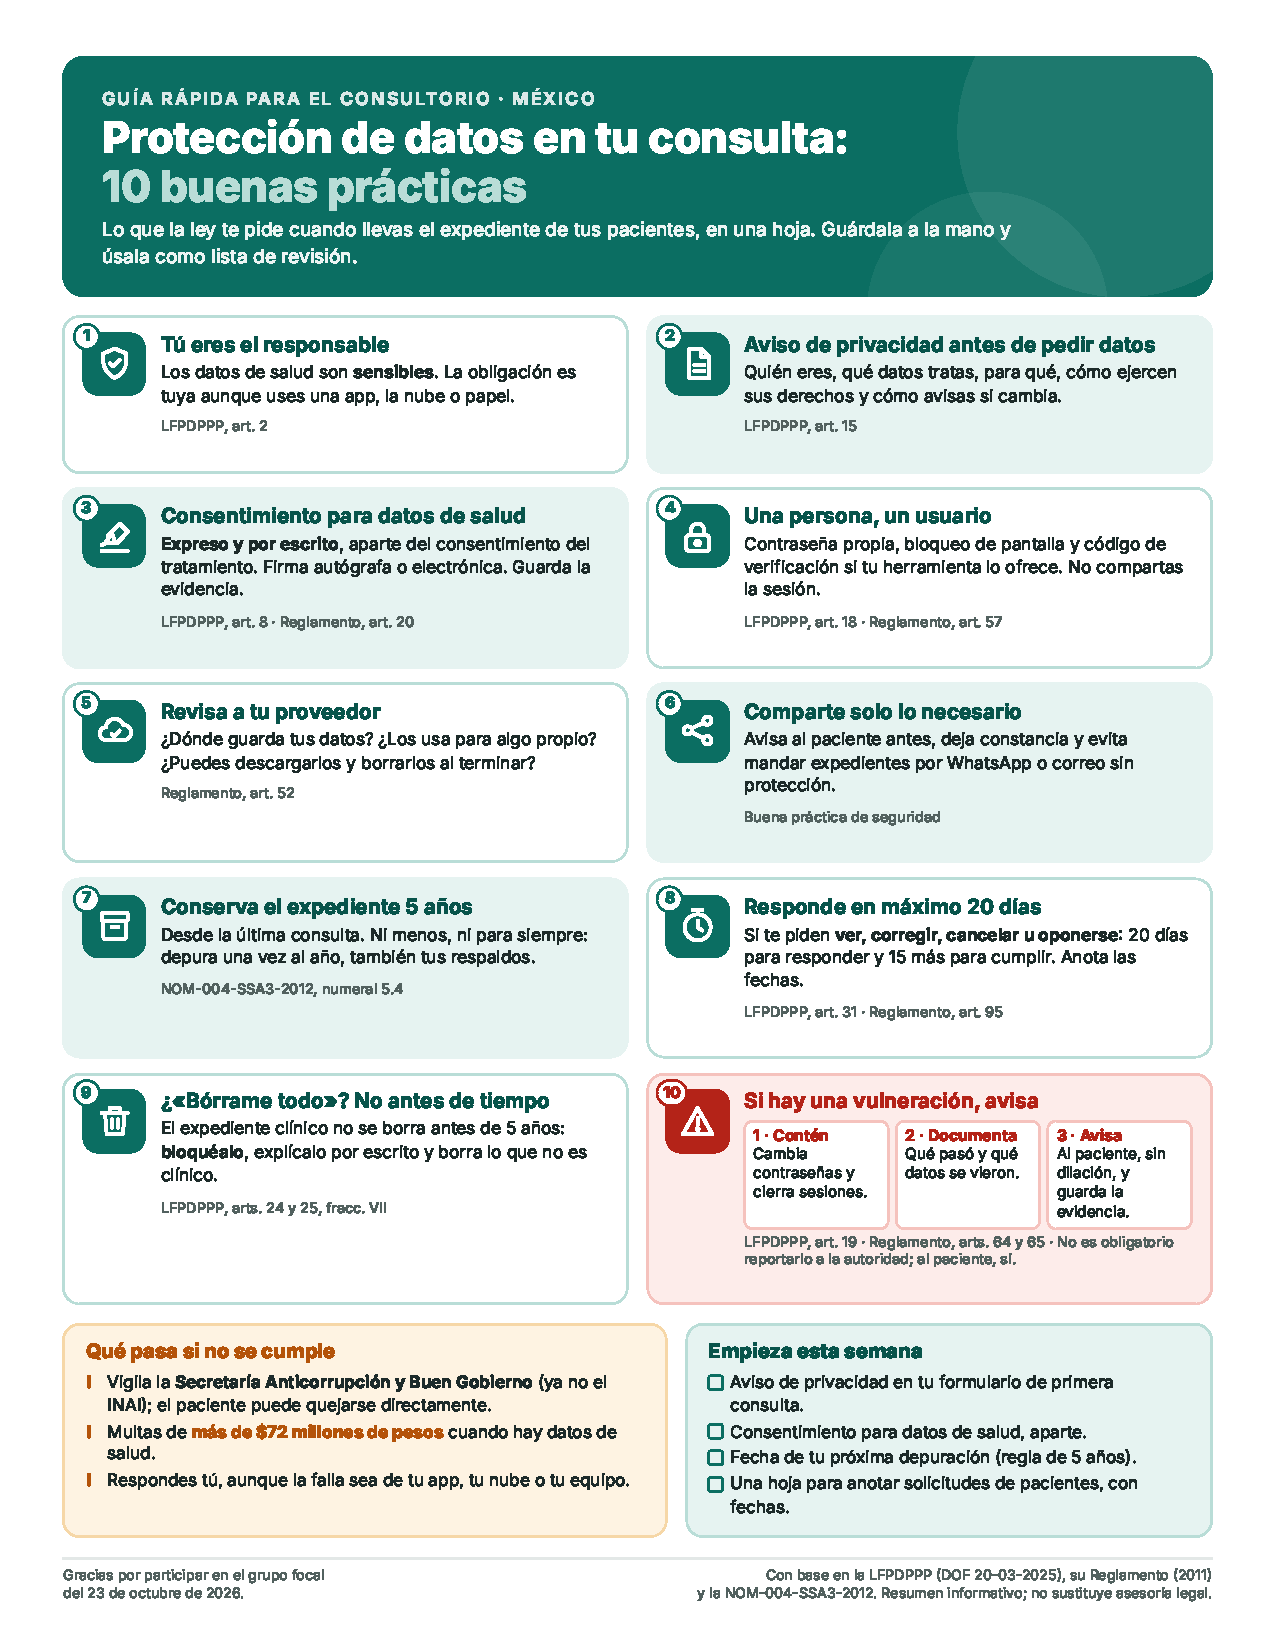
\includegraphics[width=\linewidth,height=0.8\textheight,keepaspectratio]{buenas-practicas.pdf}
  \caption{Documento de referencia entregado a los participantes del grupo focal.}
  \label{fig:buenas-practicas}
\end{figure}
% ═══════════════════════════════════════════════════════════════════════════

\section{Capturas del prototipo}
\label{anexo:capturas}
\mbox{}
% Pendiente (tras las maquetas v4): capturas de las pantallas del
% prototipo referidas en 6.2 y 6.4. Las secciones 6.2 y 6.4 ya remiten
% a este anexo como «Anexo B»; no cambiar su posición.
 
% ═══════════════════════════════════════════════════════════════════════════
\section{Uso ético de la inteligencia artificial}
\label{anexo:ia}
 
Este anexo documenta el uso de herramientas de inteligencia artificial
durante la elaboración del trabajo: en qué tareas se apoyó el autor,
con qué instrucciones, qué aportaron y cómo se conservó la dirección
del trabajo en cada paso. Sigue la estructura acordada con el tutor:
uso de las herramientas, compendio de instrucciones, síntesis del apoyo
recibido y evidencia de dirección humana.
 
\subsubsection*{Uso de las herramientas}
 
El texto del documento, el análisis normativo, el diseño de NutriApp,
las decisiones metodológicas y la interpretación de los resultados son
del autor. Las herramientas se usaron en cinco funciones. Primera, como
apoyo de redacción sobre párrafos ya escritos por el autor: sugerencias
de claridad, concisión y registro que el autor aceptó, modificó o
descartó. Segunda, como fuente de ideas y de alternativas para discutir
una decisión antes de tomarla. Tercera, para confirmar referencias,
cotejando cada cita contra la fuente oficial (la ley, el reglamento, la
norma o el comunicado citados). Cuarta, para vigilar que la idea central
del trabajo ---el nutriólogo conserva las obligaciones que la ley le
impone y NutriApp aporta los medios para cumplirlas--- se mantuviera en
todos los capítulos. Quinta, para señalar contradicciones entre partes
del manuscrito o entre el manuscrito y sus fuentes. Además, se usaron
para construir las maquetas navegables y para generar el código de
dibujo de los diagramas a partir de especificaciones escritas por el
autor. Las citas y cifras que una herramienta propuso se verificaron
contra la fuente oficial antes de integrarse; las que no pudieron
verificarse se retiraron del texto.
 
\begin{itemize}
  \item Claude (Anthropic; modelos Opus y, en la etapa final, Fable~5.1):
    sugerencias de redacción sobre texto del autor; revisión de
    consistencia entre capítulos, tablas y figuras; confirmación de
    citas contra las fuentes oficiales; en la etapa final, preparación
    de las correcciones acordadas como diferencias sobre el archivo
    \LaTeX{} del repositorio, que el autor cotejó línea por línea antes
    de integrarlas.
  \item Grok (xAI): revisión cruzada de las observaciones de la
    herramienta anterior y auditoría de inconsistencias contra el
    manuscrito; generación del código de dibujo de los diagramas de
    ingeniería del capítulo~5 y de la composición de las maquetas
    compuestas del capítulo~6, a partir de especificaciones escritas
    por el autor, que revisó cada versión.
  \item ChatGPT (OpenAI): segunda opinión, en la etapa final, sobre
    hallazgos en los que las dos herramientas anteriores no coincidían.
  \item Figma Make: construcción de las maquetas navegables descritas
    en los capítulos~4 y~6 a partir de los requerimientos del
    capítulo~6.
  \item Gemini (Google): notas de alineación entre el estudio de
    mercado y el documento.
\end{itemize}
 
Las dos primeras herramientas se usaron en contraste: cada observación
de una se sometió a la revisión de la otra, y las discrepancias se
resolvieron consultando la fuente oficial o el propio manuscrito. En la
etapa final, cada una leyó además el manuscrito completo desde varias
perspectivas de revisión (normativa, consistencia, estilo, aritmética,
referencias y metodología) y devolvió hallazgos con línea y fuente; el
autor decidió uno por uno cuáles entraban y dejó registro de cada
decisión.
 
\subsubsection*{Compendio de instrucciones}
 
Las instrucciones dadas a las herramientas fueron de cinco tipos:
(1)~revisión de estilo de un párrafo o apartado escrito por el autor;
(2)~discusión de una decisión o de una duda; (3)~confirmación de citas y
de referencias contra la fuente oficial; (4)~revisión de un capítulo o
del manuscrito completo en busca de contradicciones, con línea y fuente
para cada observación; y (5)~traducción de decisiones ya tomadas por el
autor a cambios concretos en el archivo \LaTeX{}, en los instrumentos
del grupo focal o en una figura. Las siguientes catorce instrucciones
son representativas de cada tipo; se transcriben con ajustes mínimos de
ortografía.
 
\begin{enumerate}
  \item Estilo: «Cuando te pida humanizar un párrafo, reescríbelo
    evitando las frases típicas de la inteligencia artificial, varía la
    longitud de las oraciones y prefiere el vocabulario académico
    directo. No cambies el contenido técnico, las citas ni las
    referencias; solo el estilo. Muéstrame el texto y, si te lo pido,
    también un \textit{diff} breve de qué cambiaste y por qué».
  \item Estilo: «Mantén consistencia terminológica con lo ya escrito en
    los capítulos cargados. Si algo no está en el material cargado, dilo
    explícitamente en vez de inventar».
  \item Discusión: «NutriApp no debe asumir obligaciones que la ley
    impone al profesional. No propongas funciones nuevas sin
    consultarme».
  \item Discusión: «Esto es una auditoría de ChatGPT; ya hice el
    \textit{push} con la versión que me compartiste. No lo hagas como la
    última auditoría: solo quiero saber si aplica o no y qué tendríamos
    que cambiar».
  \item Discusión: «No quiero decirle al experto qué hacer. Lo único que
    necesito es que el cierre de diez minutos vaya al final; no pongas
    tiempos, que quede abierto a su interpretación».
  \item Referencias: «¿Ya está completo solo con referencias oficiales?
    ¿Nada de foros, revistas o empresas privadas?».
  \item Referencias: «Cualquier afirmación de cambios que haya hecho
    Grok no la des por hecha; necesitamos verificarla».
  \item Contradicciones: «Quiero que corras una auditoría sin sesgo con
    revisores nuevos que solo usen el contexto para revisar, y ya
    cerrarlos».
  \item Contradicciones: «Quiero otra auditoría igual, pero que confirme
    todo lo que sí es de cambio».
  \item Contradicciones (a Grok): «Revisa el manuscrito completo.
    Reporta consistencia interna (cifras, nombres, términos, remisiones
    a secciones, tablas y figuras, contradicciones entre capítulos),
    afirmaciones sobre los nutriólogos sin cita y textos donde NutriApp
    parezca asumir obligaciones del profesional o estar ya
    implementada. Para cada hallazgo: líneas, texto actual, problema,
    fuente oficial, corrección propuesta, severidad y certeza. No
    propongas funciones nuevas. Si una fuente no abre, dilo y no
    afirmes lo que dice».
  \item Contradicciones: «Pásame un resumen para Grok, para que corra
    otra auditoría, contando lo que hayas desestimado de su revisión y
    por qué».
  \item Cambios al archivo: «¿Me puedes hacer los cambios en el .tex
    para que yo solo lo reemplace y que, al hacer el \textit{push}, solo
    se vean los cambios? Enfócate solo en los cambios; lo que esté bien,
    déjalo».
  \item Cambios al archivo: «Ya hice el \textit{push}; revísalo, que
    todo esté ahí».
  \item Instrumentos: «Necesito tres encuestas acordes con lo
    documentado en el caso: una previa, otra durante y otra de salida.
    En la de inicio debe aparecer la casilla de que va a ser anónima».
\end{enumerate}
 
El registro completo de instrucciones y respuestas se conserva en el
archivo de trabajo del autor, disponible a solicitud.
 
\subsubsection*{Síntesis del apoyo recibido}
 
El apoyo se concentró en cuatro resultados. Primero, redacción: los
párrafos del autor se revisaron en busca de frases hechas, oraciones
con más de una idea y términos usados con más de un sentido; las
sugerencias se aceptaron solo cuando no cambiaban el contenido técnico,
las citas ni las referencias. Segundo, referencias: cada cita normativa
se cotejó contra el texto oficial, lo que permitió corregir artículos
mal atribuidos (la trazabilidad, que el texto atribuía al artículo~18
de la ley y que el Reglamento prevé en su artículo~48, fracción~X,
entre las medidas del principio de responsabilidad), fechas de
publicación, y el orden y los sufijos de la lista de referencias
conforme a APA. Tercero, idea principal: en cada ronda se buscó toda
oración en la que NutriApp pareciera asumir una obligación del
nutriólogo, «cumplir» o «garantizar» la ley, o estar ya implementada,
y el autor la reformuló. Cuarto, contradicciones: se señalaron cifras,
artículos y remisiones a tablas, figuras y secciones que no coincidían
entre el resumen, los capítulos y las tablas (por ejemplo, una cifra
del INAI presentada como monto de multas cuando el comunicado reporta
inconformidades, o un término corregido en una tabla que conservaba el
sentido anterior en dos oraciones del capítulo~2), y el autor resolvió
cada una consultando la fuente. Las herramientas no produjeron el
análisis normativo, el diseño del artefacto, los casos de prueba ni la
interpretación de los resultados, y ninguna de sus observaciones entró
al documento sin la decisión expresa del autor.
 
\subsubsection*{Dirección humana y evidencia}
 
El flujo de trabajo fue el mismo durante todo el proyecto. El autor
publica una versión del manuscrito en el repositorio del proyecto; la
herramienta lee esa versión y devuelve observaciones con línea y
fuente; el autor decide cuáles atender, integra los cambios y verifica
que la versión publicada coincida con la que revisó; antes de compartir
un capítulo con el tutor, el autor lo lee completo y ajusta lo que no
corresponde a su criterio o a la dirección del trabajo. Ningún cambio
llegó al documento sin pasar por esa lectura. El historial del
repositorio conserva cada versión integrada; los dictámenes de cada
ronda de observaciones (qué entró, qué se desestimó y por qué) se
conservan con el registro de instrucciones en el archivo de trabajo del
autor; y las observaciones del tutor se atienden en un control de
cambios propio.

\end{document}
